%%%%%%%%%%%%%%%%%%%%%%%%%%%%%%%%%%%%%%%%%%%%%%%%%%%%%%%%%%%%%%%%%%%%%
%%  08 April 2002	Version 4				    					%
%%%%%%%%%%%%%%%%%%%%%%%%%%%%%%%%%%%%%%%%%%%%%%%%%%%%%%%%%%%%%%%%%%%%%
%%%%%%%%%%%%%%%%%%%%%%%%%%%%%%%%%%%%%%%%%%%%%%%%%%%%%%%%%%%%%%%%%%%%%
%%								    								%
%%  Doctoral Dissertation By Will Zhang at							%
%%	The University of Texas at Austin			     				%
%%%%%%%%%%%%%%%%%%%%%%%%%%%%%%%%%%%%%%%%%%%%%%%%%%%%%%%%%%%%%%%%%%%%%

\documentclass[12pt]{report}

\usepackage{utdiss2}	% The dissertation style as required by UT.

%%%%%%%%%%%%%%%%%%%%%%%%%%%%%%%%%%%%%%%%%%%%%%%%%%%%%%%%%%%%%%%%%%%%%
% Optional packages used for this dissertation. 					%
%%%%%%%%%%%%%%%%%%%%%%%%%%%%%%%%%%%%%%%%%%%%%%%%%%%%%%%%%%%%%%%%%%%%%

\usepackage{amsmath,amsthm,amsfonts,amscd,commath,mathtools} % Mathematic fonts
%%. and styles used in this dissertation
\DeclareMathAlphabet\mathbfcal{OMS}{cmsy}{b}{n}	% Bolded caligraphy font

\usepackage{verbatim}      	% Allows quoting source with commands.
\usepackage[utf8]{inputenc}
\usepackage{graphicx}
\graphicspath{ {images/} }

\usepackage{array,multirow,graphicx}
\newcolumntype{L}[1]{>{\raggedright\let\newline\\\arraybackslash\hspace{0pt}}m{#1}}
\newcolumntype{C}[1]{>{\centering\let\newline\\\arraybackslash\hspace{0pt}}m{#1}}
\newcolumntype{R}[1]{>{\raggedleft\let\newline\\\arraybackslash\hspace{0pt}}m{#1}}


\usepackage{etoolbox}
\apptocmd{\sloppy}{\hbadness 10000\relax}{}{}
\apptocmd{\thebibliography}{\raggedright}{}{}

\usepackage{enumitem}

\usepackage[table]{xcolor}
\definecolor{Gray}{gray}{0.9}

% Used to create the nomenclatures					%
\makeatletter

\newlength\tdima
\newcommand\tabfill[1]{%
      \setlength\tdima{\linewidth}%
      \addtolength\tdima{\@totalleftmargin}%
      \addtolength\tdima{-\dimen\@curtab}%
      \parbox[t]{\tdima}{#1\ifhmode\strut\fi}}

      
\newcommand\mytabs{\hspace*{0.5in}\=\hspace*{0.25in}\=\hspace*{0.25in}\=\hspace*{0.25in}\=\hspace*{0.25in}\=\hspace*{0.25in}\=\hspace*{0.25in}\=\hspace*{0.25in}\=\hspace*{0.25in}\=\hspace*{0.25in}\=\hspace*{0.25in}\=\hspace*{0.25in}}
\newenvironment{mynom}[1][\mytabs]
  {\begin{tabbing}#1\kill\ignorespaces}
  {\end{tabbing}}
% Used to create the nomenclatures					%
  
  
\usepackage{rotating}

\usepackage{eucal} 	 	% Euler fonts
\usepackage{makeidx}       	% Package to make an index.
\usepackage{url}		% Allows good typesetting of web URLs.

\usepackage{extdash}

\usepackage[square,numbers,sectionbib]{natbib}
\usepackage{chapterbib}

\usepackage{bibentry}


%%%%%%%%%%%%%%%%%%%%%%%%%%%%%%%%%%%%%%%%%%%%%%%%%%%%%%%%%%%%%
%%  About the Authors										%
%%%%%%%%%%%%%%%%%%%%%%%%%%%%%%%%%%%%%%%%%%%%%%%%%%%%%%%%%%%%%

\author{Will Zhang}  	% Author

\previousdegrees{B.S.}

\address{13926 Winding Cypress Brook Dr. \\ Cypress, Texas 77429}  % Address

%%%%%%%%%%%%%%%%%%%%%%%%%%%%%%%%%%%%%%%%%%%%%%%%%%%%%%%%%%%%%
%%  About the dissertation									%
%%%%%%%%%%%%%%%%%%%%%%%%%%%%%%%%%%%%%%%%%%%%%%%%%%%%%%%%%%%%%

\title{Modeling and simulating time-dependent changes in soft-tissue fabricated bioprosthetic heart valve in response to cyclic loading}

\supervisor
	{Michael S. Sacks}
    
\committeemembers
	[Aaron Baker]
	[Christopher G. Rylander]
	[Krishnaswamy Ravi-Chandar]
	{Naren Vyavahare}
    

\oneandonehalfspacequote

\topmargin 0.1in


%%%%%%%%%%%%%%%%%%%%%%%%%%%%%%%%%%%%%%%%%%%%%%%%%%%%%%%%%%%%%
%%  Macros that are needed									%
%%%%%%%%%%%%%%%%%%%%%%%%%%%%%%%%%%%%%%%%%%%%%%%%%%%%%%%%%%%%%

\newcommand{\latexe}{{\LaTeX\kern.125em2%
                      \lower.5ex\hbox{$\varepsilon$}}}

\newcommand{\amslatex}{\AmS-\LaTeX{}}

\chardef\bslash=`\\	% \bslash makes a backslash (in tt fonts)
			%	p. 424, TeXbook

\newcommand{\cn}[1]{\texttt{\bslash #1}}

\makeatletter		% Starts section where @ is considered a letter
			% and thus may be used in commands.
\def\square{\RIfM@\bgroup\else$\bgroup\aftergroup$\fi
  \vcenter{\hrule\hbox{\vrule\@height.6em\kern.6em\vrule}%
                                              \hrule}\egroup}
\makeatother		% Ends sections where @ is considered a letter.
			% Now @ cannot be used in commands.

\makeindex    % Make the index
 
 
%%%%%%%%%%%%%%%%%%%%%%%%%%%%%%%%%%%%%%%%%%%%%%%%%%%%%%%%%%%%%%%%%%%%%%
% Beginning of the document										     %
%%%%%%%%%%%%%%%%%%%%%%%%%%%%%%%%%%%%%%%%%%%%%%%%%%%%%%%%%%%%%%%%%%%%%% 
 
\begin{document}

\copyrightpage          % Produces the copyright page.

% NOTE: In a doctoral dissertation, the Committee Certification page
%		(with signatures) is BEFORE the Title page.
%	In a masters thesis or report, the Signature page
%		(with signatures) is AFTER the Title page.
%
%	If you are writing a masters thesis or report, you MUST REVERSE
%	the order of the \commcertpage and \titlepage commands below.
%
\commcertpage           % Produces the Committee Certification
			%   of Approved Version page (doctoral)
			%   or Signature page (masters).
			%		20 Mar 2002	cwm

\titlepage              % Produces the title page.

%%%%%%%%%%%%%%%%%%%%%%%%%%%%%%%%%%%%%%%%%%%%%%%%%%%%%%%%%%%%%%%%%%%%%%
% Dedication and/or epigraph are optional, but must occur here.      %
%%%%%%%%%%%%%%%%%%%%%%%%%%%%%%%%%%%%%%%%%%%%%%%%%%%%%%%%%%%%%%%%%%%%%%
%
% \begin{dedication}
% \index{Dedication@\emph{Dedication}}%
% Dedicated to my wife Shirley.
% \end{dedication}

\begin{acknowledgments}		% Optional
\index{Acknowledgments@\emph{Acknowledgments}}%
    Firstly, I would like to thank my advisor, Dr. Michael Sacks for the introducing to me to the world of biomechanics, the opportunity to work with his research group, and his patience and guidance over the years to prepare me for an academic career. Also, thank you to my committee members andthe Department of Biomedical Engineering at the University of Texas at Austin for their support throughout this process. I would also like to thank. It has been an honor to represent this department in my time here.
    

    I would like to thank my wonderful lab mates for giving me strength and support throughout this long process, lifting me up when I needed it the most. I also like to thank the post-doctoral fellows in our lab in particular, specifically Rong Fan, Chung-Hao Lee, Ankush Aggarwal and Joao Soares for their mentorship and guidance both in research and academically.
    

    Lastly, and most importantly I would like to thank my family, my parents, for raising me to the way I am, and all of the support they have given me throughout my life. I love you all.
\end{acknowledgments}

\utabstract
\index{Abstract}%
\indent
Soft-tissue-derived exogenously cross-linked (EXL) biomaterials continue to the best choice for the fabrication of bioprosthetic heart valves (BHV). Despite the ongoing research, our understanding of these materials and of the mechanisms leading to their failure remain at an empirical level. The need for advancements in modeling their behavior is further underscored by the development of percutaneously-delivered BHV devices. While these devices offer reduced surgical risk, they also present additional challenges for the design of the leaflets due to limitations in thickness and folding during delivery, resulting in a 2-year mortality rate of 33.9\% in general[2]. Thus, we seek to develop a framework for modeling and simulating soft-tissue-derived EXL biomaterials, accounting for the effects of exogenous cross-linking in permanent set and mechanical fatigue. Such approaches can significantly improve the accuracy and reliability of long-term predictions of durability and mechanical function. Firstly, we will establish the form of a nonlinear hyperelastic meso-scale structural constitutive model (MSSCM) for fibrous soft tissues, that can accurately capturing the mechanical response of common soft tissues used as a basis for EXL biomaterial. Secondly, we will study the effect of exogenous crosslinks on these tissues using glutaraldehyde (GLUT) EXL bovine pericardium. GLUT-EXLs form polymeric chains through the cross-linking process which more tightly bonds the fibers to the matrix, increasing the non-fibrous matrix stiffness and fiber-fiber interactions.  However, GLUT EXLs undergo Schiff-base reactions that lead to scission-healing behaviors that changes the geometry of BHVs. We model this effect based on first order kinetics of the scission healing reaction and validate it using static strain, cyclic strain and stress control experiments. Next, we will develop a full 3D finite element implementation of the MSSCM with the modifications for EXL for real device applications. We then parametrically examine the changes in geometry and stress distribution of BHVs overtime, exploring initial geometries and material properties which may minimize the risks of the former effects. With this, we aim to develop a better understanding of the underlying process that occurs during long-term cyclic loading through our constitutive modeling approach and device level applications, and translate the insights gained to improve BHV design and durability. 
 
\tableofcontents{}

\listoftables      % List of Tables and List of Figures will be placed
\listoffigures     % here, if applicable.

\chapter{Introduction} \index{Introduction@\emph{Introduction}}%

\section*{Preface}
\addcontentsline{toc}{section}{Preface}%

    Heart valves play a critical role of preventing back flow during cardiac operations. They are designed to withstand the demanding mechanical environment of the heart while maintaining optimal state for over 3 billion cycles. When they can no longer function properly due to fatigue, diseases or trauma, and surgical repair is not an option, surgical replacement using bioprosthetic heart valves is often the best choice. This introductory chapter focus on the current state of heart valve replacements and design, and methods for improving the durability of these devices. First, an overview of the structure and functions of heart valves is provided. Then the current state of heart valve repair and replacement is summarized, followed by the current state of bioprosthetic valve design and fabrication as well as they durability and limitations. Finally, the causes and mechanisms of bioprosthetic heart valve failure is discussed, and we outline the motivation, rationale and aims of this dissertation, on how constitutive modeling and simulations can be used to better understand bioprosthetic heart valve failure and facilitate the improvement of bioprosthetic heart valve design. 

\section{Introduction and Background}
\section{Introduction and Background}

    Cardiovascular diseases remain the leading cause of death (31.8\% of all deaths) in U.S., costing 320.1 billion each year \cite{mozaffarian_heart_2015}. One significant area that need improvements is heart valve replacement and repair procedures such as aortic valve repair using bioprosthetic heart valves (BHVs), where the mortality has not seen any major improvements since 1985 – the rate of survival after 10 years still remains only 29.7\%. Soft-tissue-derived exogenously cross-linked (EXL) biomaterials, which has only existed since the beginning of 1970s, is the dominant choice due to advantages in immunogenicity and flow dynamics over their mechanical counter parts \cite{starr_artificial_2007}. However, our understanding of these materials and of the mechanisms of their failure is still incomplete. As such, current design and development is very empirical in nature – depending on trial and error, extrapolation from accelerated wear test and long periods of clinical testing. The need for better BHV designs is further accelerated by the emergence of percutaneous devices such as the transcather aortic valve replacement (TAVR) \cite{bonow_accaha_2006}\cite{guidoin_marvel_2010}. TAVRs are an attractive alternative to open heart surgeries, especially for people at high surgical risk, as well as youths who may require multiple surgical replacements over their life-time. However, they are more often associated with peri-valvular regurgitation and is currently lacking in long-term data pertaining to their durability \cite{guidoin_marvel_2010}. Existing TAVR data suggest only 2-year mortality rate of 33.9\% \cite{kodali_two_2012} in general and 68\% for aortic valve stenosis \cite{makkar_transcatheter_2012}. Much of the existing challenges is associated with the necessary compact folded delivery system, which places additional constraints on their geometrical design and mechanical properties. It is clear that there is a strong need for a better understanding of the mechanism associated with their failure and frameworks for predicting the long-term failure of these devices.
        
    

    
    
    
    
    
    




\section{Structure and function of heart valves}
\subsection{Multi-scale structure of heart valves}

    To fully understand the functional properties of heart valves, multi-scale approaches are needed (Fig. \ref{fig:multiscalevalve}) \cite{salma_heart_2016}. This complex hierarchical structure is what lends to seamless heart valve performance under highly dynamic loading conditions. Heart valves have evolved to have multi-layered leaflet structures. The aortic valve, for example, consists of three histologically distinct layers, whereas the mitral valve has four (Fig. \ref{fig:valvelayers}). The fibrosa layer, which is located on the ventricular side of atrioventricular valves and the atrial side of semilunar valves, is composed of circumferentially aligned collagen fibers that provide the leaflets with the necessary tensile strength to open and transmit forces during coaptation while closed. The spongiosa layer is situated adjacent to the fibrosa and though it contains some collagen, its main constituents are the hydrophilic glycosaminoglycans and proteoglycans, which give the valve its compressive properties and allow it to absorb high forces during coaptation. The ventricularis and atrialis are the layers that are adjacent to blood flow in atrioventricular valvesand semilunar valves, respectively. These layers are rich in radially oriented elastin fibers and facilitate the closure movement by extending the valve leaflet as it opens and recoils when it closes. The annulus and chordae tendineae of the atrioventricular valves and the connection between the leaflets and the surrounding myocardium in the semilunar valves provide additional support. 


    Each layer contains varying amounts of collagen, glycosaminoglycan (GAG), and elastin \cite{carruthers_gene_2012}. The fibrosa layer, facing the outflow surface, consists primarily of a dense network of highly aligned type 1 collagen fibers and contributes to about 45\% of the valve thickness. The central spongiosa layer, approximately 30\% of the leaflet thickness is rich in glycosaminoglycans and water \cite{carruthers_gene_2012}. The ventricularis layer, the remaining 25\% of the leaflet faces the left ventricle inflow surface and is composed of elastin and disorganized collagen. Taken collectively, the three layers of the AV with their elastin, collagen and glycosaminoglycans constituents comprise the ECM of the valve. In addition to the biomechanical role the ECM plays in valve function, it provides a support structure for the underlying valve cell network. The ECM influences cell behavior by providing a source of ligands for cell surface receptors, which transfer mechanical strains experienced at the tissue level down to the cells and ultimately initiating intracellular signaling pathways \cite{wiltz_extracellular_2013}.


%-------------------	begin FIGURE 	-------------------%
\begin{figure}
\centering
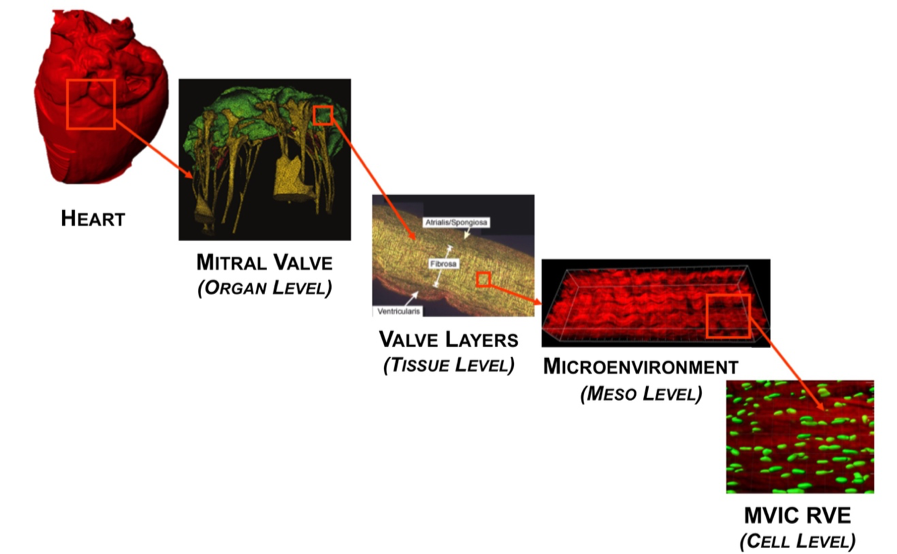
\includegraphics[width=\textwidth]{Images/chapter1/multiscalevalve.png}
\caption{The multiscale nature of heart valve biomechanics: a representation of the mitral valve at the organ-, tissue-, and cell-levels. At the tissue-level: a circumferentially oriented cross-section of the mitral valve anterior leaflet stained with Movat pentachrome, which colors collagen yellow, elastic fibers black, and hydrated PGs and GAGs blue. At the cell-level: a transmission electron micrograph of a mitral VIC from the fibrosa layer. \cite{salma_heart_2016}}
\label{fig:multiscalevalve}
\end{figure}
%-------------------	 end FIGURE 	-------------------%


%-------------------	begin FIGURE 	-------------------%
\begin{figure}
\centering
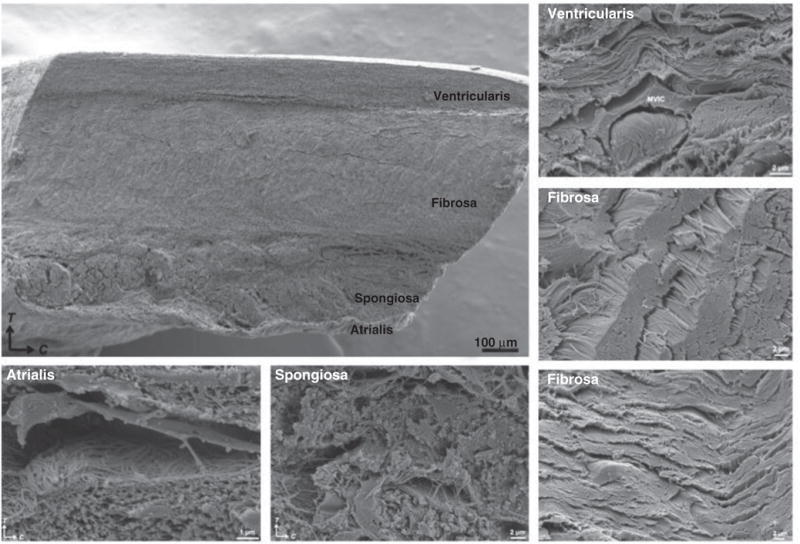
\includegraphics[width=\textwidth]{Images/chapter1/valvelayers.jpg}
\caption{Scanning electron micrograph of the multilayered microenvironment of the MV anterior leaflet. Individual micrographs of each layer are also presented: elastin-rich ventricularis and atrialis, highly collagenous fibrosa, and proteoglycan-rich spongiosa. The collagen fibrils and elastic fibers closely surround the interstitial cells and highlight the long cellular extensions. In the fibrosa, collagen fibrils are aligned in the circumferential direction of the leaflet, which is responsible for the observed anisotropy in leaflet mechanical behavior. (T: transmural, C: circumferential). \cite{salma_heart_2016}}
\label{fig:valvelayers}
\end{figure}
%-------------------	 end FIGURE 	-------------------%




\subsection{Biomechanical function of heart valves}

It has been demonstrated that the individual layers of the aortic valve are not only vastly different in their structure, but also in their mechanical behavior. Two key studies have investigated individual layer behavior of the AV leaflet. Vesely et al. observed the extensibility of intact tissue under uni-axial tension to be significantly different from the individual layer responses [71]. Stella et al. also observed measurably different behaviors under bi-axial loading of separated layers, and reported the intact tissue response to be intermediate to the separated responses [72]. Due to these consistently observed differences in layer behavior, examining the leaflet in an intact state is far more physiologically relevant. 

\section{Valvular diseases and prevalence}
\section{Valvular diseases and prevalence}

    Cardiovascular diseases are the number one killer in the United States and around the world. Heart valve treatment is a common cardiovascular surgical procedure with over 100,800 done annually in the U.S. alone \cite{mozaffarian_heart_2016} and 275,000 to 370,000 in developed nations \cite{manji_future_2012}. Calcification is the primary cause of AV failure and currently there exists no proven therapy for halting this progression. Calcified aortic valve disease is a slow, progressive, multi-factorial disorder that is more common with age, without being an inevitable consequence of aging \cite{towler_molecular_2013,freeman_management_2002,freeman_spectrum_2005,kurtz_aortic_2010,beckmann_insights_2010}. The disease is characterized by a thickening and calcification of the leaflets and is diagnosed in two stages: aortic sclerosis and aortic stenosis. aortic sclerosis, present in more than 25\% of patients over the age of 65 \cite{obrien_pathogenesis_2006}, represents the early onset of calcified aortic valve disease absent of physical obstruction to the left ventricular outflow. Aortic stenosis exists in 2-5\% of the elderly population \cite{obrien_pathogenesis_2006} is characterized by late stage obstruction and associated with impaired leaflet motion, valve tissue adaptation, and resistance to blood flow \cite{poggio_noggin_2013,grau_analysis_2012,gharacholou_aortic_2011,pflederer_aortic_2010} . Although aortic sclerosis causes significant thickening of the AV leaflets, there is little to no change in the mechanical properties of the valve, making the disease relatively asymptomatic. Recent statistics have shown that within 10 years of their initial diagnosis, 10\% of aortic sclerotic patients reach a state of severe calcified aortic valve disease that requires immediate AV replacement once symptoms emerge \cite{gharacholou_aortic_2011}. 
    
    
    Aortic stenosis has been identified as the end-stage of calcified aortic valve disease that progresses from the microscopic early changes of aortic sclerosis to, in a subset of patients, asymptomatic and then symptomatic Aortic stenosis \cite{kurtz_aortic_2010,otto_calcific_2010,aikawa_look_2012}. Once aortic sclerosis is detected, there is an increased risk of cardiovascular events. In early Aortic stenosis, when mild symptoms begin to present, survival rates deviate much more than expected and decline dramatically with the onset of severe symptomatic Aortic stenosis. Over the last decade, several clinical trials, mostly extensions of atherosclerosis-related studies, have been performed to halt the progression of calcified aortic valve disease with randomized studies showing substantial equivalence between treatments and placebo \cite{parolari_do_2011,moura_rosuvastatin_2007,cowell_randomized_2005,benton_statins_2009,rossebo_intensive_2008}. However, there are currently no pharmacological therapies available to treat calcified aortic valve disease symptomatic patients that are considered superior to full valve replacement surgery. 




\section{Surgical repair and replacement}


\section{Heart valve prosthesis}

\subsection{Brief history of the development of heart valve replacements}

\subsection{Advantages of tissue-engineered valves}

\subsection{Fabrication of bioprosthetic heart valves}

\subsection{Current and future technology on bioprosthetic heart valves}




\section{Bioprosthetic heart valve durability and limitations}

\subsection{Bioprosthetic heart valve life-span}

\subsection{Limitations in bioprosthetic heart valve design and fabrication}


\section{Causes of bioprosthetic heart valve failure}

\subsection{Biological and mechanical aspects of fatigue}

\subsection{Brief summary on the role of calcification}

\subsection{Mechanical fatigue and failure}

\section{Motivation, rationale, and specific aims}

    Soft-tissue-derived exogenously cross-linked (EXL) biomaterials continue to play an important role in surgical repair and medical devices. This is especially true for bioprosthetic heart valves (BHV), by having advantages in immunogenic and mechanical behaviors [1]. Despite ongoing research, our understanding of these materials and of the mechanisms leading to their failure remains at an empirical level. The need for advancements in predicting the material behavior is further underscored by the development of percutaneously-delivered BHV devices. While these devices reduce surgical risk, they also present additional challenges for the design of the BHVs due to limitations in thickness, and folding and compression during delivery. A significant challenge prohibiting accurate and predictive simulations of BHVs are a lack of understanding of the effect of exogenous cross-linkers, such as glutaraldehyde (GLUT), and an associated predictive material model in response to cyclic loading. GLUT EXLs form polymeric chains through the cross-linking process which more tightly bond the collagen fibers to the non-fibrous matrix, increasing the non-fibrous matrix stiffness and fiber-fiber interactions. However, GLUT EXLs also undergo Schiff-base reactions that are hypothesized to lead to scission-healing behaviors that result in the permanent set (PS) phenomena. PS continuously changes in the reference geometry of the BHV and can induce extra-physiological stress concentrations in the BHV leaflets. Microstructural-based constitutive models for tissues and their use in valve-level simulations can lead to insights into the underlying mechanisms and more accurate prediction of their long-term performance. Thus, we seek to develop a framework for modeling and simulating biologically-derived EXL soft collagenous tissues for BHV, accounting for the effects of EXL, PS, and collagen fiber-level damage, taking the following approach:


    \subsubsection*{Specific Aim 1: Establish and validate a generalized nonlinear hyperelastic meso-scale structural constitutive model (MSSCM) for native collagenous soft tissues.} As a first step towards modeling EXL biomaterials, we will take a generalized meso-scale (at the level of the constituent fibers) structural modeling approach to accurately model the mechanical response of soft tissues. Firstly, we will develop an improved analytical method for processing extant mechanical data under generalized 2D deformations, to more accurately characterize the tissue. Next, after posing the model form, we will extensively validate critical assumptions such as affine fiber deformation, mechanical response of the constituent fibers, and direct integration of physical measurements of the fiber microstructure. The validation will be done through extensive mechanical characterization through different testing methods and microstructural characterization at the 1) micro-scale (fibril) and 2) meso-scale using optical techniques such as multiphoton microscopy and x-ray scattering. The two tissues we will examine for application and validation of the model are the ovine pulmonary artery and the porcine mitral valve leaflets, which offer a diverse selection structural composition to span applicable realms.
    
    \addcontentsline{toc}{subsubsection}{Specific Aim 1: Establish and validate a generalized nonlinear hyperelastic meso-scale structural constitutive model for native collagenous soft tissues.}%


    \subsubsection*{Specific Aim 2: Extend the MSSCM to account for of the presence of EXLs and subsequent response to continuous cyclic loading.} Using GLUT treated bovine pericardium, we aim to separately model the mechanical response of the collagen fibers, matrix, and fiber-fiber interactions due to cross-linking. For this, we will develop a method to map the collagen fiber architecture characterized from the native state to the EXL state. Next, we will develop a PS model based on a constantly evolving referential configuration that occurs due to scission-healing when the tissue is held in an extended state. We will validate the model for orientation and strain level dependence. The model will be tested and validated using constant cyclic strain, as well as stress control experimental data. Finally, we will extend the model for collagen fiber-level damage that may occur during cyclic loading. 
    
    \addcontentsline{toc}{subsubsection}{Specific Aim 2: Extend the meso-scale structural constitutive model to account for of the presence of EXLs and subsequent response to continuous cyclic loading.}%
    
    
    \subsubsection*{Specific Aim 3: Application to organ/device level}. In this final aim, we will develop a full 3D finite element implementation utilizing the open source FEniCS framework for greater modularity and extensibility. The model will utilize real BHV geometries and fiber microstructure mapped from experimental measurements, and will be validated by simulating of the PS experiments from SA 2. We will further perform organ-level study of PS and collagen fiber-level damage using accelerated wear testing of specialized ovine mitral transcutaneous BHVs. We will use an inverse modeling approach with micro-CT measurements [2] to quantify changes in mechanical behaviors. The validated model and rate constants will then be used to parametrically examine the changes in BHV geometry and stress distribution overtime, where change in resting and loaded geometry of the valve as well as the development of stress concentrations are the early indicators of BHV failure. We will also explore initial geometries and material properties which may minimize the risks of these effects. With this, we aim to develop a better understanding of the underlying process that occurs during long-term cyclic loading using our constitutive modeling approach and device level applications, and translate the insights gained to improving BHV design and durability. 

    \addcontentsline{toc}{subsubsection}{Specific Aim 3: Application to organ/device level}%

\bibliographystyle{plainnat}
\bibliography{phd}





\chapter{Structural constitutive models for planar collagenous soft tissues}


\section*{Preface}
\addcontentsline{toc}{section}{Preface}%

    Fundamental to developing a deeper understanding of soft tissue function and pathology is the development of an accurate tissue-level constitutive model. In the present work, we developed a novel meso-scale (i.e. at the level of the fiber, 10-100 $\mu$m in length scale) structural constitutive model (MSSCM) with application to MV leaflet. This model takes into account the layered structure of these tissues and the contributions from the distinct collagen and elastin fiber networks within each tissue layer. The requisite collagen and elastin fibrous structural information for each layer was quantified using second harmonic generation microscopy and conventional histology. A comprehensive mechanical data set was also used to guide the model formulation and parameter estimation. Furthermore, novel to tissue-level structural constitutive modeling approaches, we allowed the collagen fiber recruitment function to vary with orientation. Finally, a novel fibril-level (0.1 to 1 $\mu$m) validation approach was used to compare the predicted collagen fiber/fibril mechanical behavior with extant MV small angle X-ray scattering data. Results demonstrated excellent agreement, indicating that the MSSCM fully captures the tissue-level function. Future utilization of the MSSCM in computational models of the MV will aid in producing highly accurate simulations in non-physiological loading states that can occur in repair situations, as well as guide the form of simplified models for real-time simulation tools.

\textbf{The work contained in this chapter was published as}:  Zhang, W.; Ayoub, S.; Liao, J. \& Sacks, M. S.
A meso-scale layer-specific structural constitutive model of the mitral heart valve leaflets 
Acta Biomater, 2016, 32, 238-55 


%---    INTRODUCTION
\section{Introduction}
    
    The mitral valve (MV) is the most structurally complex and physically demanded valve within the heart. It is one of the most suitable choices for the development and validation of a generalized meso-scale structural constitutive model (MSSCM). According the American Heart Association in 2013, it is estimated that MV disease is present in over 4 million adults \cite{go_heart_2014}. MV regurgitation is the most common pathology resulting from myocardial infarction (ischemic mitral regurgitation or IMR). The most frequent corrective approach used to restore leaflet function is MV annuloplasty \cite{kaneko_mitral_2014, amini_vivo_2012}, wherein an annuloplasty ring is used to induce MV leaflet closure during systole. However, such procedures alter the distribution of stress within the leaflet \cite{amini_vivo_2012,salgo_effect_2002,mahmood_three_2009,jimenez_saddle_2007,padala_saddle_2009,sacks_vivo_2006,eckert_vivo_2009,rausch_vivo_2011}, which may influence the long-term durability of the repair procedure. Long-term studies suggests that 60\% of patients who underwent MV repair show recurrence of MV regurgitation within 3–5 years, and 10–15\% of patients require re-operation within the following 10 years \cite{flameng_recurrence_2003,flameng_durability_2008}. The need for computational models, based on understanding of the underlying mechanobiological processes is self-evident for predicting the outcome of surgically repaired MVs and driving the development of improved patient-specific surgical techniques.
    
    
    While MV leaflets may first appear essentially to be membranous flaps, they are in actuality complex multilayered structures that undergo large anisotropic deformations in vivo \cite{sacks_vivo_2006}. Specifically, there are four morphologically distinct layers of the MV: the ventricularis, fibrosa, spongiosa, and atrialis \cite{carruthers_alterations_2012}. All layers are composed of various amounts of dense networks of collagen (mostly type I) and elastin fibers, as well as non-fibrous proteoglycans (PG) and glycosaminoglycans (GAG). In a recent study \cite{lee_quantification_2015}, we demonstrated that the layer-specific deformations of the MV interstitial cells (MVIC) are a direct result of the layer-specific architectures. This suggests that layer-specific adaptations are possible, as observed in Wells et al.\cite{wells_physiological_2012}. Yet, it remains unclear as to (1) why the MV has this distinct pattern of layers, (2) what the respective mechanical roles of each layer are, and (3) how does these patterns relate to the bulk macro-scale responses.
    
    
    The underlying layer-specific differences in mechanical properties are a result from the constituent fiber populations. Type I collagen is the most abundant protein found in MV tissue, and it is the major determinant of its mechanical behavior \cite{parry_molecular_1988,gelse_collagens_2003}. The functional subunit of collagen is the collagen fibril, which composed of tropocollagen molecules that arrange themselves into a quarter stacking array \cite{parry_molecular_1988,gelse_collagens_2003}. It is this structure that allows small angle X-ray scattering (SAXS) studies to measure the underlying fibril deformations for tendon \cite{sasaki_elongation_1996,sasaki_stress_1996} and MV leaflet tissues \cite{liao_relation_2007}. At the next structural level, the collagen fibrils group to form collagen fibers. There is an incomplete understanding regarding the functional relationship between collagen fibers and the fibrils. In fact, the exact definition of collagen fibers in relation to fibrils is usually tissue specific. Like the fibrils from which their functional properties are derived, collagen fibers exhibit tensile strength of up to 1 GPa \cite{shen_stress_2008,gentleman_mechanical_2003,eppell_nano_2006,yang_mechanical_2008,sacks_biomechanics_2009} with low flexural stiffness \cite{sacks_biomechanics_2009}. As a result, collagen fibers typically extend by no more than a 4–5\%. To increase the tissue-level compliance, collagen fibers at the macroscopic scale become sinusoidally crimped \cite{parry_molecular_1988} and does not contribute mechanically until fully straightened. Moreover, the distribution of collagen fiber-level straightening strains is the mechanism for tissue-level non-linearity \cite{lanir_constitutive_1983,sacks_multiaxial_2003}. 
    
    
    In contrast to collagen, elastin forms complex cross-linked fibrous networks with comparatively low modulus that are thought to assist in tissue recoil \cite{debelle_elastin_1999,debelle_structures_1999} and maintaining collagen fiber crimp \cite{vesely_comparison_1998,scott_aortic_1995}. Unlike large arteries, elastin is present in much lower quantities in valvular tissues compared to collagen \cite{sacks_biomechanics_2009,vesely_comparison_1998,lis_biochemical_1987,stella_biaxial_2007} and its role in valve mechanics is not well understood. Finally, we note that glycosaminoglycans (GAGs) are known to affect water retention and hysteresis in valvular tissues \cite{lovekamp_stability_2006,eckert_biomechanical_2013}, with the loss of GAGs known to reduce cuspal thickness and diminish rehydration capacity. However, GAGs are not a primary load bearing component, but appear act as a dampening mechanism to smooth rapid bending motions of the leaflet during valve function \cite{eckert_biomechanical_2013}.
    
    
    Thus, a more complete understanding of MV function and failure must involve an improved understanding of how the above MV leaflet structures mechanically interact. This is best done through the mathematical development of constitutive models that incorporate these features, which can aid both in providing insight and in forming a predictive modeling framework for their remodeling and failure. In the present, work we developed a novel comprehensive meso-scale (i.e. at the level of the fiber) structural constitutive model (MSSCM) for MV leaflets, focusing on the specific collagen and elastin fiber networks within each of its four distinct layers. We used a comprehensive set of structural and mechanical studies (Table \ref{c2tab:experiments}) and a rigorous experimentally guided approach to tackle model formulation, parameter optimization and model validation (Fig. 1). The results were then validated at both the micro (fibril) and tissue-level using a novel approach based on a previous SAXS study on the mitral valve \cite{liao_relation_2007}, and again at the meso-scale using measured fiber structures. We also explored a novel extension to previous structural constitutive model approaches \cite{hollander_constitutive_2011,chen_micromechanics_2011,fata_insights_2014,sacks_incorporation_2003} to allow for angular dependency of collagen fiber recruitment (orientation-variant) and assessed the model predictive capabilities under extra physiological loading that could occur in post-surgical scenarios.
    
\begin{table}\label{c2tab:experiments}
\centering
\caption{Experimental Techniques and Deliverables}
 \begin{tabular}{|m{.2in}|L{0.6in}|L{1in}|L{2.5in}|L{0.95in}|}
 \hline
 &  \textbf{Study}  & \textbf{Description}  & \textbf{Purpose}  & \textbf{Description}  \\
 \hline
 
 \multirow{2}{0.2in}{\rotatebox[origin=c]{90}{Structural}}
 & SHG  
 & Image of fluorescently labeled collagen and elastin 
 & Image processing is done to quantify the fiber orientation distribution function of collagen and elastin within each layer. 
 & ODF (used for validation) \\
 \cline{2-5}
 
 & Histology
 & Collagen, elastin and Proteoglycans are stained in a transmural slice. 
 & The image is separated into channels and is used to quantify the mass fractions and relative fraction of collagen and elastin of each layer. This is used directly in the model. 
 & Mass fractions   \\
 \hline
 
 \multirow{1}{0.2in}{\rotatebox[origin=c]{90}{Mechanical}}
 & SAXS
 & X-ray scattering at a length comparable to D-period of the fiber
 & The SAXS scatter pattern have periods related to the D-period of the collagen fibers. The D-period can be used to quantify the fiber-level strain and the fiber stiffness
 & Collagen Fiber Modulus, (for validation)   \\
 \cline{2-5}
 
 & Planar Biax (EB)
 & Biax with equal strain along both axes
 & Under equibiaxial strain, we can recover the ensemble stress from the sum of the axial stresses. This allows us to model the ensemble stress directly to determine the fiber modulus and fiber recruitment.
 & \multirow{1}{0.95in}{Collagen Fiber Modulus, Recruitment Parameters (For validation)}  \\
 \cline{2-4}
 
 & Uniaxial	
 & Tissue is deformed along the preferred direction of the fibers
 & With the tight splay, under uniaxial extension all fibers become nearly aligned to the test axis, allowing us to use a simplified model rather like using the ensemble stress to recover the fiber modulus and recruitment. 	& \\
 \cline{2-5}
 
 & Planar Biax (Multi-prot)	
 & Data is taken over the physiological and extra-physiological range.	
 & This with us the data to performed parameter estimation to determine the properties of the MV. The outer extra-physiological protocols can be used check the predictive ability of the model. 
 & Layer dependent material properties.     \\
 \hline
 
 \end{tabular}
\end{table}

%---    METHODS
\section{Methods}

\subsection{General consideration and assumptions}\label{sec:generalconsiderations}

\subsubsection{Collagen fibrils and fibers} \label{sec:collagenconsiderations}

    In the present work, we assumed that the collagen fibrils were contiguous subunits of the collagen fibers, so that there was negligible slippage between fibrils. To characterize the straightening behavior of the fiber-level crimped structure \cite{lanir_constitutive_1983, fata_insights_2014, sacks_incorporation_2003, lanir_structural_1979, kastelic_structural_1980, hansen_recruitment_2002, cacho_constitutive_2007, grytz_constitutive_2009}, we use only the fiber axial stretch needed to fully straighten the fiber, slack stretch, rather than the period and amplitude of the collagen fibers. This avoids the necessity of incorporating detailed unloaded geometry for the collagen fibers.


    In most structural models, the distribution of collagen slack strains (the recruitment distribution) is assumed to be independent of the orientation. This approach has the advantage of allowing collagen fiber recruitment model parameters to be determined directly from a single planar equibiaxial strain (EB) tests, where the deformation gradient tensor is $F = \operatorname{diag}[\lambda, \lambda, 1/\lambda^2$] and no fiber rotations occur (e.g. \cite{fata_insights_2014}). For bovine pericardium, we have shown that when the collagen fiber orientation distribution function (ODF) is obtained independently, the complete in-plane response can be predicted \cite{sacks_incorporation_2003}. However, some angular dependence may be physiologically relevant for general tissues. For example, collagen fibers are constantly produced and degraded under physiological stresses, and generally prefer to function within homeostatic stress levels \cite{humphrey_cardiovascular_2002}. Moreover, MV leaflets experience large and highly anisotropic deformations in vivo, which would induce substantially higher fiber ensemble stresses in the larger strain direction \cite{amini_vivo_2012,sacks_vivo_2006}. We thus speculate that collagen fibers may exhibit larger undulations in the directions of larger physiological strain to maintain a constant fiber ensemble stress. However, the exact dependence of collagen recruitment on fiber orientation remains unknown and has yet to be explored in the literature.
    
    
    For the collagen fiber material model, a stress–strain relation that is linear in 2nd Piola Kirchhoff stress and Green Lagrange strain is the predominant fiber model of choice [40], [41], [47]. However, SAXS studies of intact tissue shows that the fibril strain varies linearly with applied forces in tendon [18], [19] and MV leaflet tissues [20], [21]. Furthermore, the results are corroborated by the atomistic modeling results by Buehler [48], where the force displacement relation is essentially linear at strains lower than 0.35.
    
    
    For the collagen fiber material model, a stress–strain relation that is linear in 2nd Piola Kirchhoff stress and Green Lagrange strain is the predominant fiber model of choice \cite{sacks_incorporation_2003,lanir_structural_1979,fan_simulation_2014}. However, SAXS studies of intact tissue shows that the fibril strain varies linearly with applied forces in tendon \cite{sasaki_elongation_1996,sasaki_stress_1996} and MV leaflet tissues \cite{liao_relation_2007}. Furthermore, the results are corroborated by the atomistic modeling results by Buehler \cite{buehler_atomistic_2006}, where the force displacement relation is essentially linear at strains lower than 0.35.
    



\subsubsection{Elastin fiber network} \label{sec:elastinconsiderations}

    Elastin fibers function through an entropy-driven process wherein the decrease in entropy drives the increase in fiber stress as the fiber is elongated. As of yet, there is no first-principle form for elastin when modeled either as a continuous phase or a discrete fibrous network. Typical MV models are either purely phenomenological or ignore the elastin component entirely. In a previous study on ovine pulmonary artery \cite{fata_insights_2014}, we found the elastin fibers to behave linearly in second Piola–Kirchhoff stress and Green Lagrange strain. However, the specific form of the elastin likely depends on a variety of factors including cross-linking and residual strain. Moreover, it is not clear if there are layer-specific differences, and thus a more general material model for the MV elastin fiber network is needed.




\subsubsection{Affine kinematics and layer averaged responses}

    As in previous structural approaches, we assume affine fiber kinematics. This assumption is supported by a recent study wherein we demonstrated that the MV anterior leaflet collagen and elastin fibers all deformed in a manner consistent with affine deformation kinematics \cite{lee_presence_2015}. We further assume each layer is structurally homogeneous (i.e. ignore intra-layer structural variations). Thus, and in order to derive the total individual layer response as a function of its collagen and elastin components, the following information was used (Table \ref{c2tab:experiments}):
        \begin{enumerate}
            \item The mass composition of each layer, including the quantities of collagen and elastin.
            \item The ODF for the collagen and elastin fibers within each layer.
            \item The recruitment behaviors of the collagen fiber network for each layer.
        \end{enumerate}
    Finally, the following assumptions were made according to the current understanding of heart valve leaflet tissues:
        \begin{enumerate}
            \item All layers are tightly bonded with no slippage, similar to what is observed in the aortic valve leaflet \cite{buchanan_interlayer_2013}.
            \item There are no mechanical interactions between layers and that they deform with the bulk tissue.
            \item The collagen fiber modulus is the same for all layers and that the differences in collagen mechanical contribution response are due to variations in structural organization.
            \item Fiber–fiber interactions are negligible.
            \item Fiber–matrix interactions are negligible.
        \end{enumerate}




%%%%%%%%%%%%%%%%%%%%%%%%%%%%%%%%%%%%%%%%
\subsection{Constitutive model formulation}

\subsubsection{Single fiber models}

    Based on the above considerations (Section \ref{sec:collagenconsiderations}), the following linear force displacement relation for the collagen fibrils and fibers was used
        %-------------------	begin EQUATION 	-------------------%
        \begin{equation}\label{eqn:collagenfiberlaw}
        \begin{aligned}
        P_f =& \eta_{C}\left(\lambda_t - 1\right)\frac{1}{\lambda_s} = \frac{\eta_C}{\lambda_s}\left(\frac{\lambda_f}{\lambda_s} - 1\right)    \\
        S_f =& \frac{1}{\sqrt{2E_s + 1}}\left( \frac{1}{\sqrt{2 E_s + 1}} - \frac{1}{\sqrt{\sqrt{2E_f + 1}}}\right)
        \end{aligned}
        \end{equation}
        %-------------------	 end EQUATION 	-------------------%
    where $P_f$ and $S_f$ are the 1st and 2nd Piola Kirchhoff fibers stresses, $\eta_C$ is the collagen fiber modulus, $\lambda_f$ and $E_f$ are the fiber stretch and Green’s strain, $\lambda_t$ and $E_t$ are the true fiber stretches and Green’s strains, and $\lambda_s$ and $E_s$ are the slack fiber stretches and Green’s strains. For the elastin fibers, based on Section \ref{sec:elastinconsiderations} and our previous work on the pulmonary artery \cite{fata_insights_2014}, we use the following generalized form,
        %-------------------	begin EQUATION 	-------------------%
        \begin{equation}\label{eqn:elastinfiberlaw}
        \begin{aligned}
        S^e_f = \eta_e \left( E^e_f\right)^d
        \end{aligned}
        \end{equation}
        %-------------------	 end EQUATION 	-------------------%
    Here $\eta_e$ is the elastin fiber modulus and $d$ is the exponent that determines the degree of non-linearity of the fiber. This allows us to alter the stress strain relationship of the fiber based on the mechanical and structural data acquired.




\subsubsection{Fiber ensemble models}

    As in previous works \cite{lanir_constitutive_1983,sacks_incorporation_2003,fan_simulation_2014}, we scale up to the tissue-level by first considering an ensemble of collagen fibers, which is defined as a sub-group of fibers that share a common initial orientation $n_0$. Collagen fiber recruitment is commonly assumed to be independent of $n_0$, i.e. is orientation-invariant \cite{fata_insights_2014,sacks_incorporation_2003,lanir_structural_1979,fan_simulation_2014}. To evaluate the hypothesis that there may be angular variations is due to homeostasis (Section \ref{sec:collagenconsiderations}), we developed the following generalized framework for orientation-variant fiber recruitment. The fiber recruitment distribution function $D\left[E_s(n_0)\right]$ is a function of the fiber slack strain $E_s$ and orientation $n_0$, and is represented by a beta distribution function. $D\left[E_s(n_0)\right]$ was parametrized by a mean $\mu_r$, a standard deviation $\sigma_r$, and was defined over a strain range bounded by the lower- and upper-bounds $E_{lb}$ and $E_{ub}$. The general form given by,
        %-------------------	begin EQUATION 	-------------------%
        \begin{equation}\label{eqn:recruitmentdistribution}
        \begin{aligned}
        D(\mathbf{\xi},E_s) = \frac{(y)^{\alpha-1}(1-y)^{\beta-1}}{B(\alpha,\beta)(E_{ub}-E_{lb})}, 
            \quad y = \frac{E_s - E_{lb}}{E_{ub} - E_{lb}}, \quad y \in (0,1)
        \end{aligned}
        \end{equation}
        %-------------------	 end EQUATION 	-------------------%
    where the parameter vector is $\mathbf{\xi} = \{\mu, \sigma, E_{lb}, E_{ub} \}$. Here, $B(\alpha, \beta)$ is the Beta distribution function with shape parameters $\alpha$, $\beta$. The interrelationships between the two are
        %-------------------	begin EQUATION 	-------------------%
        \begin{equation}\label{eqn:recruitmentparameters}
        \begin{gathered}
        \hat{\mu}_r = (\mu_r - E_{lb})/(E_{ub} - E_{lb}), \quad \hat{\sigma}_r = \sigma_r/(E_{ub} - E_{lb}),  \\
        \alpha = \frac{-\hat{\mu}_r (\hat{\sigma}_r^2 + \hat{\mu}_r^2 - \hat{\mu}_r)}{\hat{\sigma}_r^2}, \quad \beta = \frac{(\hat{\mu}_r - 1) (\hat{\sigma}_r^2 + \hat{\mu}_r^2 - \hat{\mu}_r)}{\hat{\sigma}_r^2}, \\
        \mu_r \in (E_{lb}, E_{ub}), \quad \Hat{\mu}_r \in (0,1)
        \end{gathered}
        \end{equation}
        %-------------------	 end EQUATION 	-------------------%
    It should be noted that the parameters in Eqns \ref{eqn:recruitmentdistribution}, \ref{eqn:recruitmentparameters} are functions of the initial fiber ensemble orientation $n_0$, so that $\xi (n0)$.


    While comprehensive, equations \ref{eqn:recruitmentdistribution}, \ref{eqn:recruitmentparameters} present difficulties in actual implementation by either direct experimental measurement or parameter estimation \cite{hill_theoretical_2012}. However, the equations can be reduced using the assumption that the ensemble stresses are constant with orientation. Here the ensemble strain Es is scaled by the maximum ensemble strain $E_{max}(\mathbf{n}_0)$ in the fully loaded state.
        %-------------------	begin EQUATION 	-------------------%
        \begin{equation}\label{eqn:recruitmentasafunctionofangle}
        \begin{aligned}
        D(\mathbf{\xi},E_s) = \bar{D}\left(\bar{\mathbf{\xi}}, \frac{E_s}{E_max(\mathbf{n}_0)}\right)
        \end{aligned}
        \end{equation}
        %-------------------	 end EQUATION 	-------------------%
    where the parameter vector is now $\bar{\mathbf{\xi}} = \bar{\mathbf{\xi}}(\mathbf{n}_0) = (\bar{\mu}, \bar{\sigma}, \bar{E}_{lb}, \bar{E}_{ub})$, which is non-dimensionalized as indicated by the overbar. Using this form, the same fraction of fibers is recruited for each fiber ensemble at the maximum strain and the ensemble stresses becomes approximately constant with orientation. This form also requires no additional parameters. In addition to the above analysis, we utilized the standard orientation-invariant approach \cite{fata_insights_2014} defined as
        %-------------------	begin EQUATION 	-------------------%
        \begin{equation}\label{eqn:recruitmentasafunctionnormal}
        \begin{aligned}
        D(\mathbf{\xi},E_s) = D(\{\mu_r, \sigma_r, E_{lb}, E_{ub}\}, E_s(\mathbf{n}_0))
        \end{aligned}
        \end{equation}
        %-------------------	 end EQUATION 	-------------------%
    For both forms, the resulting ensemble stress is given by
        %-------------------	begin EQUATION 	-------------------%
        \begin{equation}\label{eqn:collagenensemblestress}
        \begin{aligned}
        &S_e^{ens}\left[ \mathbf{\xi}, E_{ens}(\mathbf{n}_0)\right] = 
            \eta_C \int_0^{E_{ens}(\mathbf{n}_0)} \frac{D(\xi,x)}{\sqrt{2x+1}} 
                \left(\frac{1}{\sqrt{2x+1}} - \frac{1}{\sqrt{2E_{ens}(\mathbf{n}_0)+1}}\right)  \\
        &\mathrm{where} \quad D(\mathbf{\xi}, x) = 
            \begin{cases} 
                \bar{D}(\bar{\mathbf{\xi}},x,\mathbf{n}_0) & \text{orientation variant} \\
                D(\mathbf{\xi},x) & \text{orientation invariant} 
            \end{cases}
        \end{aligned}
        \end{equation}
        %-------------------	 end EQUATION 	-------------------%
    Finally, since elastin fibers are straight (i.e. not undulated like collagen fibers), the elastin ensemble stress is simply $S_e^{ens} = \eta_e(E_{ens})^d$.
    



\subsubsection{Complete layer and full tissue forms}

    The strain energy of collagen and elastin fibers for each layer is given by the sum of the fiber ensembles weighted by the fiber ODF $\Gamma(\theta)$ and mass fraction with respect to each layer $\phi$. $\Gamma(\theta)$ is approximated using another beta distribution function with a mean $\mu$ and standard deviation $\sigma$ \cite{fata_insights_2014}. Since $\Gamma(\theta)$ is nearly symmetric, the shape parameters $\alpha$ and $\beta$ are forced to be equal (Eqn. \ref{eqn:recruitmentparameters}), thus $\bar{\mu} = 0.5$ at all points. A remainder function is then used to ensure $\theta \in \left[\mu - \pi/2, \mu + \pi/2 \right]$, before normalizing it to the domain of the beta function $y \in \left[0,1\right]$, yielding
        %-------------------	begin EQUATION 	-------------------%
        \begin{equation}\label{eqn:orientatinodistributionfunction}
        \begin{aligned}
        \Gamma(\theta) = \frac{B(\alpha,\alpha,y)}{\pi}, \quad y = \frac{\operatorname{Mod}(\theta - (\mu -     \pi/2), \pi)}{\pi}, \\
        \alpha = -0.5 \left(\bar{\sigma}^2 + 0.25 -0.5\right)/\bar{\sigma}^2, \quad \bar{\sigma} = \sigma/\sigma\pi
        \end{aligned}
        \end{equation}
        %-------------------	 end EQUATION 	-------------------%
    where $B$ is the Beta function.
    
    
    Next, we define the tissue “matrix” as PG, GAGs, and water into a homogenized single phase and represented using an incompressible Neo–Hookean model. The resulting matrix stress tensor, assuming a planar configuration and no distinctions between layers, is $S_m = \mu_m(\mathbf{I} - C_{33}\mathbf{C}^{-1})$. This phase is necessary to enforce incompressibility and to obtain accurate results in computational simulations \cite{fan_simulation_2014}. The resulting total tissue stress, weighted by the mass fractions $\phi$, is given by
        %-------------------	begin EQUATION 	-------------------%
        \begin{equation}\label{eqn:multilayeredstressform}
        \begin{aligned}
        \mathbf{S} =& \sum_{L = 1}^\mathrm{n layers} \left\{
        \begin{array}{l}
        \phi_c^L\eta_c\int_{-\pi/2}^{\pi/2}\Gamma_c^L(\theta)\int_0^{E_{ens}(\theta)} \frac{D_L(x,\theta)}{\sqrt{2x+1}}\left( \frac{1}{\sqrt{2x+1}} - \frac{1}{\sqrt{2E_{ens}(\theta)+1}} \right) \mathbf{n}_0\otimes\mathbf{n}_0 \dif x\dif\theta\\
        + \phi_e^L\eta_e^L\int_{-\pi/2}^{\pi/2}\Gamma_e^L(\theta)(E_{ens})^{d_L} \mathbf{n}_0\otimes\mathbf{n}_0 \dif\theta
        \end{array}
        \right\}    \\
        &+ \phi_m\eta_m\left(\mathbf{I} - C_{33}\mathbf{C}^{-1}\right)
        \end{aligned}
        \end{equation}
        %-------------------	 end EQUATION 	-------------------%
    where the superscript L indicates the layer and the parameter list for Eqn. \ref{eqn:multilayeredstressform} is given in Table \ref{c2tab:modelparameters}.


\begin{table}
\centering
\caption{Experimental Techniques and Deliverables}\label{c2tab:modelparameters}
\begin{tabular}{L{.15in}L{0.2in}C{0.3in}L{2.8in}L{1.0in}}
\hline
& \multicolumn{2}{c}{\textbf{Parameter}}
& \textbf{Description}  
& \textbf{Layer}   \\
\hline

\multirow{12}{*}{\rotatebox[origin=c]{90}{Collagen}}
& 1    & $\eta_c$  & Mean collagen fiber modulus   &  \\
\cline{2-5}
& 2    & $\sigma_c^f$   & \multirow{2}{2.7in}{Standard Deviation of the collagen fiber ODF}  & Fibrosa   \\
& 3    & $\sigma_c^a$   &   & Atrialis  \\
\cline{2-5}
& 4    & $\mu_c^f$      & \multirow{3}{2.7in}{Mean of the collagen fiber recruitment distribution} & Fibrosa    \\
& 5    & $\mu_c^a$      &   & Atrialis    \\
& 6    & $\mu_c^s$      &   & Spongiosa    \\
\cline{2-5}
& 7    & $\sigma_r^f$   & \multirow{3}{2.7in}{Standard deviation of the collagen fiber recruitment distribution} & Fibrosa    \\
& 8    & $\sigma_r^a$   &   & Atrialis    \\
& 9    & $\sigma_r^s$   &   & Spongiosa    \\
\cline{2-5}
& 10   & $E_{ub}^f$     & \multirow{3}{2.7in}{The upper-bound of the collagen fiber recruitment distribution} & Fibrosa    \\
& 11   & $E_{ub}^a$     &   & Atrialis    \\
& 12   & $E_{ub}^s$     &   & Spongiosa    \\
\cline{2-5}
\hline

\multirow{8}{*}{\rotatebox[origin=c]{90}{Elastin}}
& 13    & $\sigma_e^v$   & \multirow{2}{2.7in}{Standard deviation of the elastin fiber ODF}  & Ventricularis   \\
& 14    & $\sigma_e^a$   &   & Atrialis  \\
\cline{2-5}
& 15    & $\eta_e^f$      & \multirow{3}{2.7in}{Mean elastin ensemble modulus} & Ventricularis    \\
& 16    & $\eta_e^a$      &   & Atrialis    \\
& 17    & $\eta_e^s$      &   & Spongiosa    \\
\cline{2-5}
& 18    & $d_e^f$      & \multirow{3}{2.7in}{Mean elastin ensemble exponent} & Ventricularis    \\
& 19    & $d_e^a$      &   & Atrialis    \\
& 20    & $d_e^s$      &   & Spongiosa    \\
\hline

\multirow{2}{*}{\rotatebox[origin=c]{90}{Matr.}}
& 21    & $\eta_m$  & Mean matrix shear modulus	homogenized over all four layers   &  \\
& 22    & $\mu_\theta$  & Preferred direction of the mitral valve leaflet relative to the testing axes		   &  \\
\hline
\end{tabular}
\end{table}







%%%%%%%%%%%%%%%%%%%%%%%%%%%%%%%%%%%%%%%%
\subsection{Structural characterization} \label{c2sec:structure}

    To obtain the mass fractions of the major ECM components for each layer, additional porcine MV leaflets (n = 3) were harvested from a local slaughter house and immediately transported for sectioning. Transverse sections from the central region of each leaflet were stained using Movat’s Pentachrome stain (Fig. \ref{c2:fig:2}), and then imaged using light microscopy to determine the relative thickness of each layer. Color deconvolution was then used to separate the collagen (yellow), elastin (Black), and PGs (Blue). The relative area fraction in each layer was determined using the total color intensity (Table \ref{c2tab:massfractions}). ODFs for both collagen and elastin fiber networks were quantified by SHG imaging using methods described by Carruthers et al. \cite{carruthers_alterations_2012} (Fig. \ref{c2:fig:2}). The resulting orientation distribution functions (ODF) for collagen and elastin were obtained using the methods of Courtney et al. \cite{courtney_design_2006}.
    
    


%%%%%%%%%%%%%%%%%%%%	begin FIGURE 	%%%%%%%%%%%%%%%%%%%%
\begin{figure}
\centering
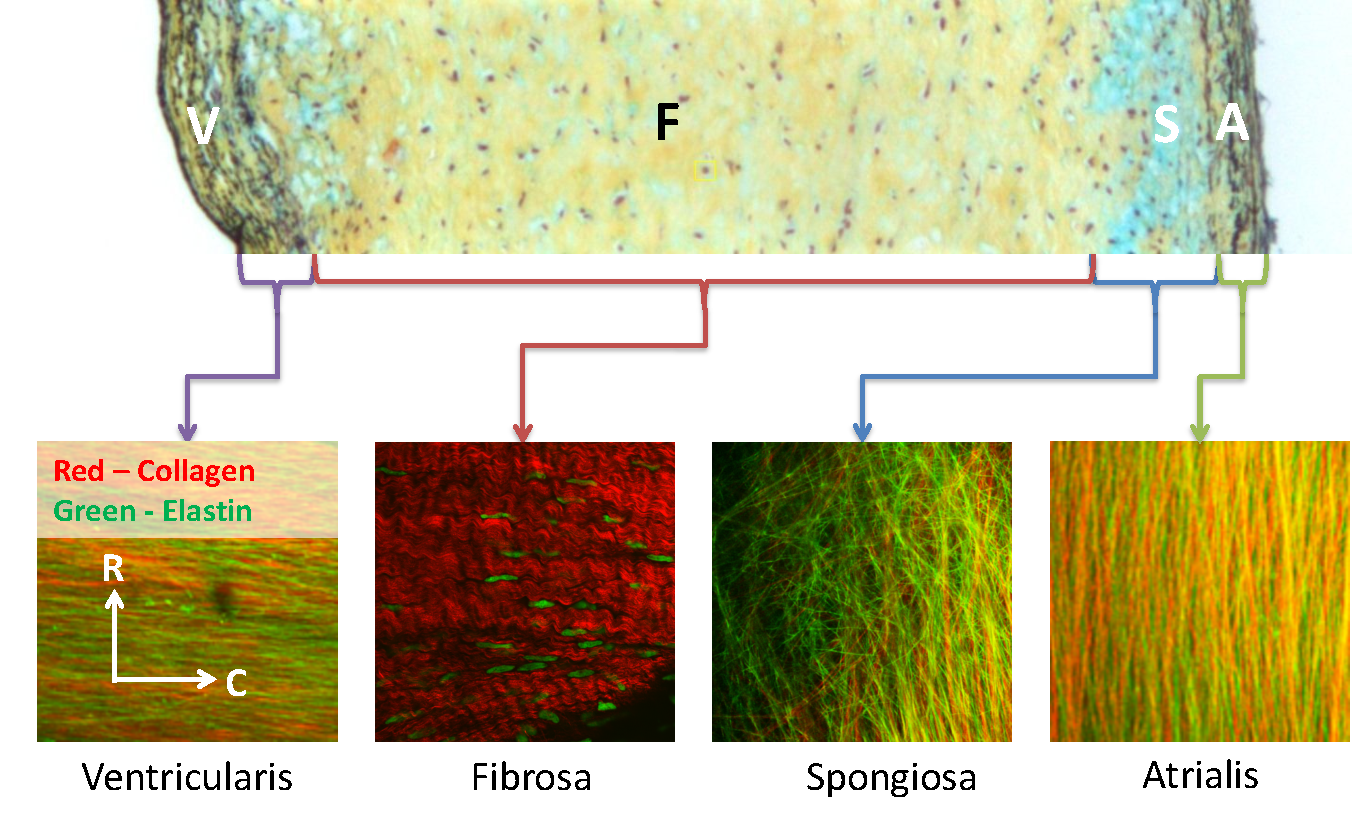
\includegraphics[width=\textwidth]{Images/chapter2/figure2.pdf}
\caption{Microstructural analysis was done using Movat pentachrome stain of the transverse-radial section of the center region of the MV anterior leaflet (Top), and multiphoton microscopy (MPM) of the ventricularis (V), fibrosa (F), spongiosa (S) and atrialis (A) layer of the anterior leaflet (Bottom). The histological section shows the relative thickness of each layer, and the MPM shows the orientation or collagen (red) and elastin (green) fibers in each layer.}
\label{c2:fig:2}
\end{figure}
%%%%%%%%%%%%%%%%%%%%	 end FIGURE 	%%%%%%%%%%%%%%%%%%%%



    
\begin{table}
\centering
\caption{Volume fractions of ECM components in MV (unitless)}\label{c2tab:massfractions}
\begin{tabular}{L{.65in}L{0.65in}L{1.05in}L{0.875in}L{0.875in}L{0.875in}}
\hline
\textbf{Leaflet} & \textbf{ECM} & \textbf{Ventricularis} & \textbf{Fibrosa} & \textbf{Spongiosa} & \textbf{Atrialis}   \\
\hline

\multirow{2}{*}{Anterior}
& Collagen  & $0.078\pm0.018$   & $0.839\pm0.021$   & $0.036\pm0.015$   & $0.047\pm0.007$   \\
& Elastin   & $0.487\pm0.039$   & $0.066\pm0.030$   & $0.067\pm0.000$   & $0.380\pm0.036$   \\
\hline
\multirow{2}{*}{Posterior}
& Collagen  & $0.068\pm0.008$   & $0.778\pm0.052$   & $0.043\pm0.018$   & $0.110\pm0.044$   \\
& Elastin   & $0.104\pm0.021$   & $0.067\pm0.017$   & $0.118\pm0.036$   & $0.711\pm0.035$   \\
\hline
\end{tabular}
\end{table}

\subsection{Experimental mechanical studies} \label{c2:sec:mechanicalstudies}

    In order to develop a comprehensive model to simulate the leaflets in both physiological and surgically altered/pathological conditions, it is necessary to explore the MV properties beyond the physiological range. Moreover, no single deformation mode can provide all the data needed for parameter optimization. Thus, the following deformation modes were utilized.


\subsubsection{Uniaxial loading}

    Under uniaxial loading along the circumferential direction, only the highly circumferentially aligned collagen in the fibrosa and ventricularis layers, which constitute the bulk of the MV, are loaded. This aided the preliminary examination of the collagen fibers mechanics, as the contribution of elastin becomes negligible at high stress. To perform these tests, specimens from four anterior MV leaflets were tested under uniaxial strain until failure. Each specimen was cut into 5 by 20 mm stripes with the long axis oriented along the preferred direction (circumferential) of the leaflet. The specimens were clamped at both ends of the long axis with a separation of 13.5 mm to serve as the gauge length. The transverse direction was unconfined and allowed to contract laterally. One end of the clamps was then displaced at a rate of 0.1 mm/s. The tests were manually aborted after the tissue tears. No preconditioning was done and the tissue was not preloaded. To measure the internal strains more accurately, an optical marker tracking method was used \cite{billiar_biaxial_2000}. All testing was done at room temperature in phosphate buffered saline (PBS).


\subsubsection{Equibiaxial planar strain tests}

    EB planar strain kinematics has several important advantages for examining the effective stress–strain relations in MV leaflet tissues. Firstly, like uniaxial testing, the test can be carried out into the MPa range, exceeding physiological stress levels to insure all collagen fibers are fully recruited. Secondly, as there are no fiber rotations, one can obtain the fiber ensemble response under the assumption of orientation-invariant fiber recruitment \cite{fata_insights_2014,sacks_incorporation_2003,fan_simulation_2014}. This allows direct estimation of the orientation-invariant fiber recruitment function and effective fiber modulus.
    
    
    To obtain the requisite EB strain data, porcine MV specimens were harvested from a local slaughter house and immediately transported for testing. 10 mm by 10 mm sections were taken from the center region of each leaflet and mounted to a custom-built biaxial device \cite{grashow_biaxial_2006,grashow_planar_2006} with the circumferential and radial directions aligned to the device axes. The specimens were immersed in PBS and tested at room temperature. The strain was determined via four fiducial markers glued to the central region of the specimen \cite{billiar_biaxial_2000}. The free-floating state was used as the stress-free reference state, while a preload of 1 g was applied for testing purposes. Starting at 10\% strain, each specimens was tested for ten 30 s cycles with the tenth cycle taken as representative. The maximum strain was then systematically increased until a linear stress–strain region was observed. A total of 7 anterior and 7 posterior porcine MV leaflets were tested.


\subsubsection{Full in-plane responses}

    To obtain the necessary mechanical data for full parameter estimation, a comprehensive set of planar biaxial mechanical data was obtained that encompassed the extra-physiological range. Porcine MV specimens were harvested using a protocol similar to the EB strain testing above. Following mounting, these specimens were first preconditioning for 10 cycles at 90 N/m. The specimens were then unloaded, and the post-preconditioned free-floating state was used as the stress-free references state. Similar to the above, a preload of 1 g was applied for testing purposes. For each loading path, the specimens were loaded to a maximum membrane tension of 90 N/m for ten 30 s cycles with the last cycle taken as representative \cite{grashow_biaxial_2006,grashow_planar_2006}. Circumferential ($x_1$) to radial ($x_2$) ratios of $P_{11}:P_{22}$ = 1:2, 3:4, 1:1, 4:3, and 2:1 were used, with two additional extreme loading protocols that represented extra-physiological ranges of 1:10 and 10:1 to evaluate the MSSCM predictive capabilities.
    
    
\subsubsection{Collagen fiber ensemble analysis using SAXS}

    One way we can assess the intrinsic mechanical properties of collagen fibers, dissociated from the effects of crimping, is using fibril-level measurements from SAXS. We thus utilized extant data from a porcine MV study by Liao et al. \cite{liao_relation_2007} to validate the collagen modulus and recruitment. The experiment was performed on MV anterior leaflets specimens, which were loaded under EB stress. SAXS was used at each load step to measure the fibril strain. Experimental details have been provided in \cite{liao_relation_2007}.
    



\subsection{Parameter estimation}

\subsubsection{General considerations}

    Obtaining the true global cost-function minimum can become exceptionally difficult for highly nonlinear models with a large number of parameters, such as equation \ref{eqn:multilayeredstressform}. This will often include issues such as parameter covariance and the presence of local minima. We thus developed the following detailed sequential procedure for parameter estimation using observations from the structure of the MV leaflet (Section \ref{c2sec:structure}).
    
    
    Firstly, the ventricularis is rich in both elastin and collagen, with a relatively narrow ODF and a preferential orientation in the circumferential direction for both fiber types (Fig. \ref{c2:fig:2}). Secondly, the fibrosa, comprising the bulk of the MV leaflet, contains mainly collagen fibers highly aligned to the circumferential direction with almost no elastin except for trace amounts near the spongiosa. Thirdly, the spongiosa contains relatively small amounts of elastin and collagen, both of which are randomly oriented, and is predominately composed of PGs and GAGs. Fourthly, the atrialis contains the largest population of elastin and some collagen, both of which has a narrow ODF and oriented along the radial direction. Fifthly, since the collagen and elastin fibers in the ventricularis and fibrosa were observed to have very similar ODFs, they cannot be separated reliably from a parameter optimization standpoint. Thus, the small amount of elastin in the fibrosa was considered part of the ventricularis elastin, and the collagen in the ventricularis was considered part of the fibrosa collagen. Also, since the collagen and elastin fibers in the ventricularis and fibrosa were found to be identically aligned and orthogonal to the atrialis, their respective preferred directions were fixed during parameter estimation.
    
    
\subsubsection{Modifications for collagen fiber recruitment bounds}

    As observed in both uniaxial and EB strain data (Fig. \ref{c2:fig:3}), a gradual increase in collagen fiber recruitment and a transition to a linear stress–strain response were clearly visible. In preliminary studies of the collagen fiber recruitment probability function $D(E_s)$, we observed that when the lower-bound $E_{lb}$ was sufficiently distant from the mean $\mu_r$, the overall shape of $D(E_s)$ did not change significantly with further decreases in $E_{lb}$. Thus, to reduce the number of parameters, the lower-bound of the distribution was set to $E_{lb} = 0$.
    
    
%%%%%%%%%%%%%%%%%%%%	begin FIGURE 	%%%%%%%%%%%%%%%%%%%%
\begin{figure}
\centering
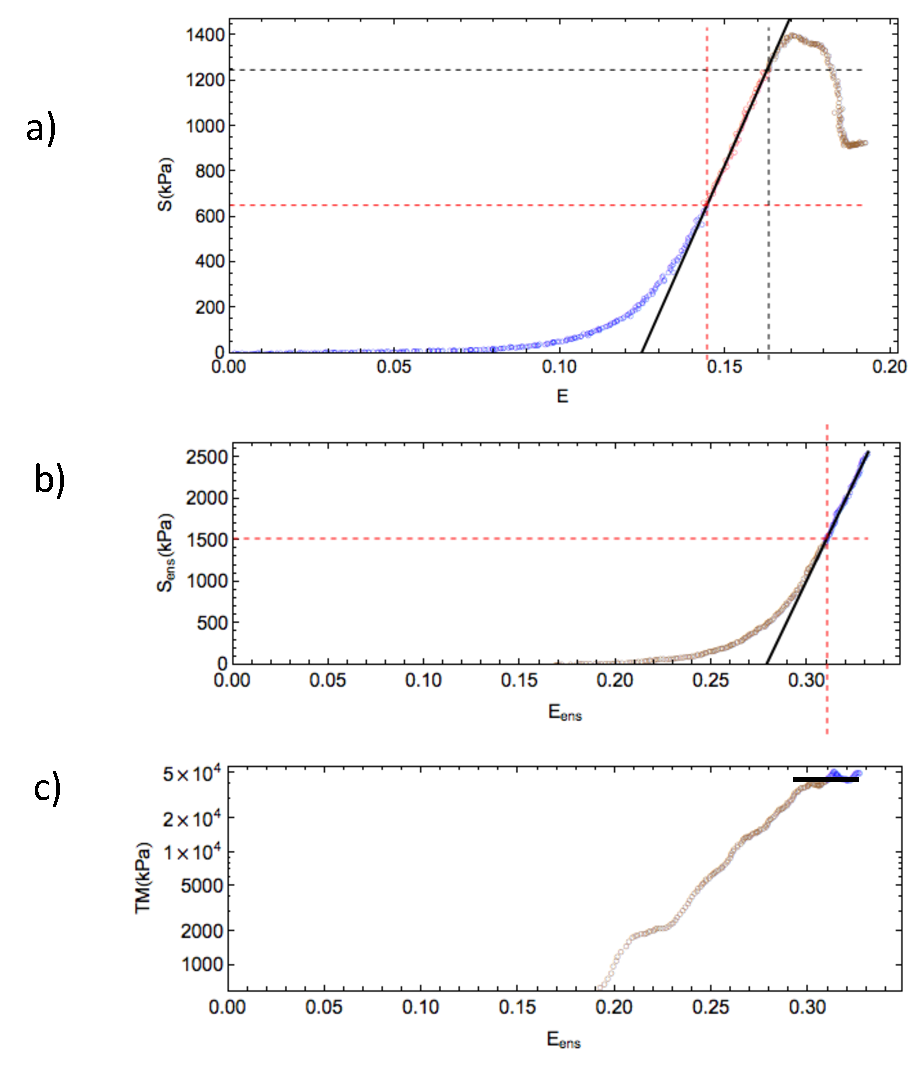
\includegraphics[width=0.95\textwidth]{Images/chapter2/figure3.pdf}
\caption{Example mechanical testing result of (a) uniaxial and (b) and (c) equibiaxial strain test data from an anterior leaflet. The linear post recruitment region is shown by the black line, which indicates full collagen fiber recruitment. The (c) tangent modulus curve in equibiaxial strain test shows a clear flattened section in the post-transition region. Tangent modulus curve for uniaxial extension is not shown due to similarities.}
\label{c2:fig:3}
\end{figure}
%%%%%%%%%%%%%%%%%%%%	 end FIGURE 	%%%%%%%%%%%%%%%%%%%%




\subsubsection{Elastin fiber model} \label{c2:sec:elastinfibermodel}

    To determine the elastin fiber model (Sections \ref{sec:elastinconsiderations} Elastin fiber network, \ref{sec:collagenconsiderations} Single fiber models), we utilized the low stress region of the mechanical response. Due to the collagen fiber recruitment, we can retroactively determine the Elb of the recruitment distribution as the point when the cumulative distribution is less than 1\% (typically less than 3–8 kPa). Since collagen does not contribute significantly in this region, the response in this region can be considered entirely due to elastin (Fig. \ref{c2:fig:4}a). In pilot studies, we found that $d>1$ in equation \ref{eqn:elastinfiberlaw}. In fact, the exponent for the ventricularis and atrialis layer appeared to be different. Thus, we allowed d to vary during parameter estimation rather than being a set to a constant value.


%%%%%%%%%%%%%%%%%%%%	begin FIGURE 	%%%%%%%%%%%%%%%%%%%%
\begin{figure}
\centering
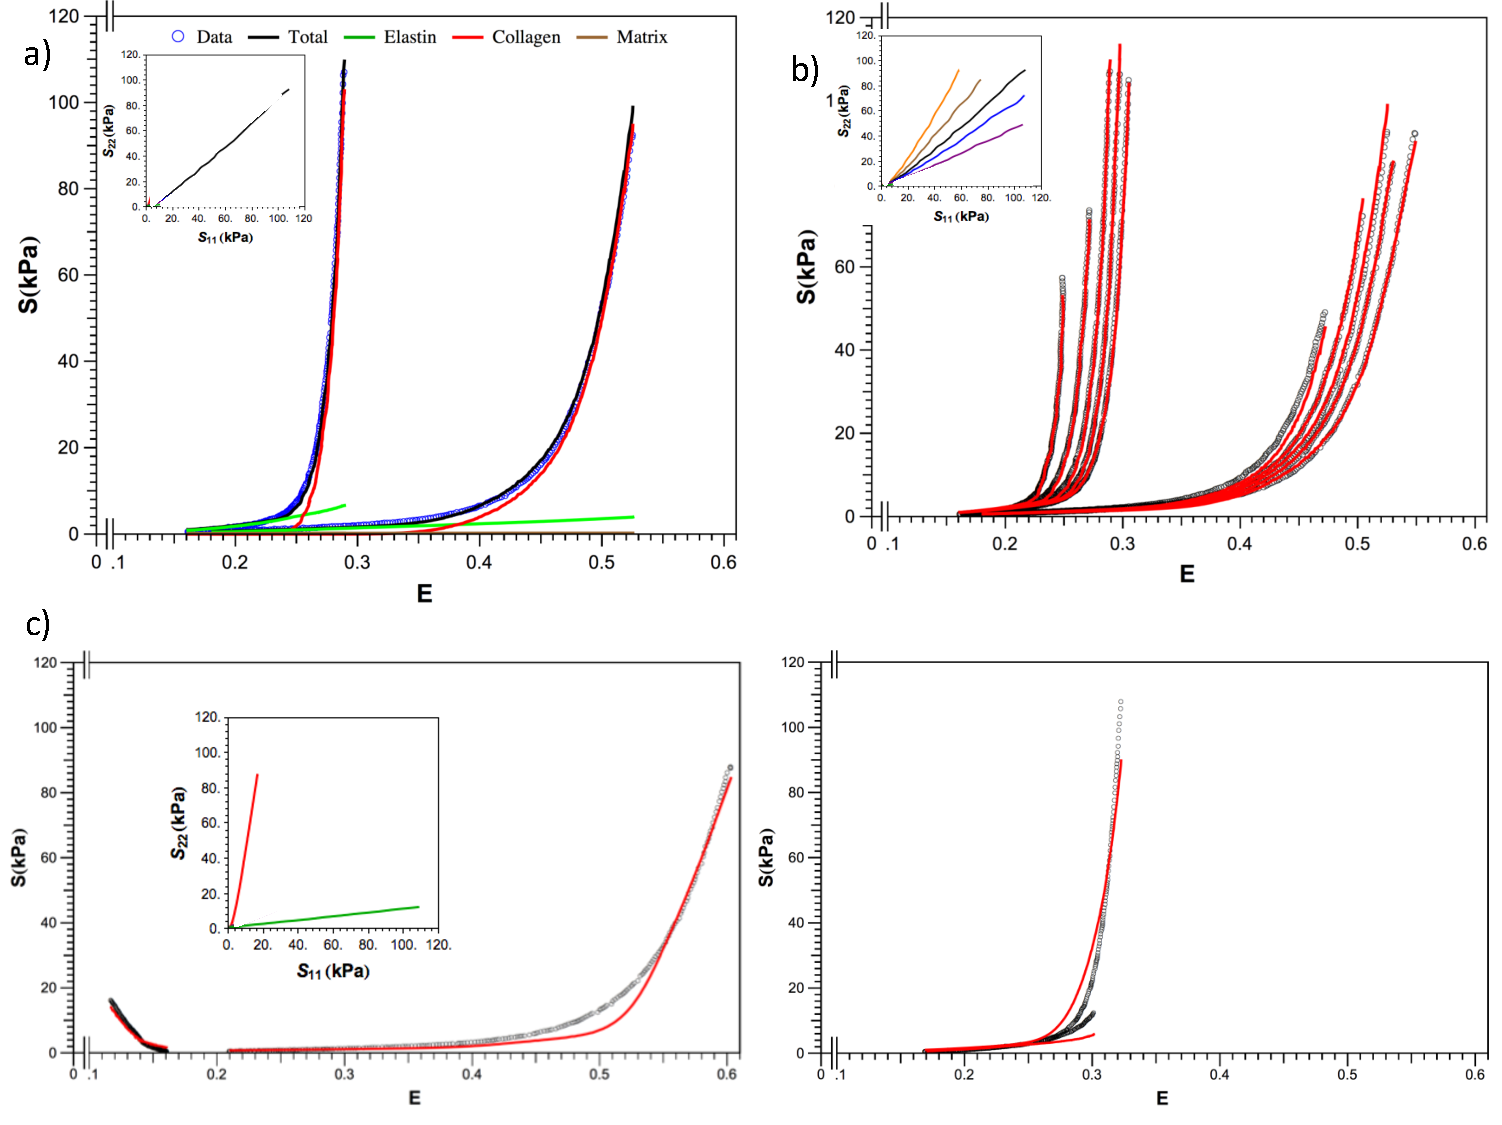
\includegraphics[width=\textwidth]{Images/chapter2/figure4.pdf}
\caption{Example of the best fit from an anterior leaflet. The (a) equibiaxial stress protocol was fit with only the elastin (green) first, followed by fitting the collagen only while keeping the elastin fixed. (b) The final fit of all “physiological” protocols are shown. (c) The two extra-physiological protocols, which were not fit, is show. This suggests that the model have good predictive capability.}
\label{c2:fig:4}
\end{figure}
%%%%%%%%%%%%%%%%%%%%	 end FIGURE 	%%%%%%%%%%%%%%%%%%%%




\subsubsection{Parameter estimation part 1 – collagen fiber recruitment} \label{c2:sec:2254}

    From the above analysis, the number of parameters was reduced to 22 (Table \ref{c2tab:modelparameters}). To start of the parameter estimation, we took advantage of the simplified kinematics of the uniaxial and EB test data to isolate the effects of collagen fiber recruitment in a simplified fiber recruitment model. For both datasets, the collagen fiber network in the fibrosa and ventricularis were idealized as a family of uni-directionally aligned fibers, with the elastin fibers neglected as their contributions to the total stress were insignificant in this loading state. Also note that for the EB tests the fiber ensemble stress can be determined directly by \cite{sacks_biaxial_2000}.
        %-------------------	begin EQUATION 	-------------------%
        \begin{equation}\label{c2eqn:ensembleform}
        \begin{aligned}
        S_{ens} = S_{11} + S_{22} \quad \text{for} \quad E_{11} = E_{22}, E_{12} = 0
        \end{aligned}
        \end{equation}
        %-------------------	 end EQUATION 	-------------------%
    We assumed in this first step that the recruitment distribution is orientation invariant, so that the collagen recruitment function $D(\mathbf{\xi},E_s) = D(\{\mu_r, \sigma_r, E_{lb}, E_{ub}\})$. $E_{ub}$ was determined by the transition point to the linear region (Fig. \ref{c2:fig:3}), leaving only $\mu r$, $\sigma r$ to be fit in this part of the parameter estimation. 
    
    
\subsubsection{Parameter estimation part 2 - full planar biaxial mechanical data set}

    Ideally, the measured ODFs $\Gamma(\theta)$ from the same specimen should be directly inserted into Eqn. \ref{eqn:multilayeredstressform}. However, in practice, we found that the ODFs had to be fitted to adjust for the specimen to specimen variability. Nevertheless, the mean best fitted ODFs can be compared to the mean measured ODFs to ensure that the estimate parameters are reasonable comparing to the true value. We expedited the process by assuming that the ODFs for each specimen is not significantly different from the true measured mean ODFs. Thus, the mean ODFs can be used as an initial guess and speed up the convergence to the optimal value. The use of a global algorithm will also ensure the optimized parameters do not become trapped at the mean value. Similarly, the estimated recruitment distribution $D(\mathbf{\xi}, x)$ is also obtain from independent specimens. The recruitment distribution parameters $\mathbf{\xi}$ are again used only as initial guesses and parameter validation.
    

    Taking a similar approach to Fata et al. \cite{fata_insights_2014}, we first examined the equibiaxial stress protocol ($P_{11}:P_{22}$ = 1:1), which is the best approximation of the in vivo loading state of the MV. The low stress region as defined in section \ref{c2:sec:elastinfibermodel} was used to fit the elastin (Fig. \ref{c2:fig:4}a). This is easily identified as the nearly linear response before the exponential like collagen response. Furthermore, due to limitations concerning the elastin model form, where the elastin response can increase exponentially to unrealistically surpass the response of the collagen, the exponent parameter d for the elastin (Table \ref{c2tab:modelparameters}) was constrained to be less than 3.5. Next, the remaining high stress region was used to fit the collagen fiber response independently. Using this coupled approach, we were able to minimize the search space to the 12 parameters associated with collagen (Table \ref{c2tab:modelparameters}). Once a reliable estimate of the parameters was obtained for this protocol, the inner 3 protocols (3:4, 1:1, 4:3) were fit using the existing parameters as the initial guess. We then progressed to the remaining “physiological” protocols (1:2, 3:4, 1:1, 4:3, 2:1) once again keeping the previous parameters as the initial guess to obtain better estimated parameters.
    
    
    Preliminary attempts demonstrated that gradient algorithms were unable to converge to the proper solution and tended to become unable to handle local minimas. As a result, we employed the genetics-based differential evolution algorithm to perform the optimization, similar to Fata et al. \cite{fata_insights_2014}. To narrow down the search space and guide the optimization, initial guess was derived from the above mechanical studies (Section \ref{c2:sec:mechanicalstudies}). Parameter estimation was performed using a custom program written in Mathematica (Wolfram Research Corp.).
    




\subsection{Model validation} \label{c2:sec:26}

    The mean fitted fiber ODFs $\Gamma(\theta)$ from each layer of the MV anterior leaflet were compared to the measured ODFs obtained from SHG imaging (section \ref{c2sec:structure}). Since the orientation of the fibers are referenced to the laboratory testing or imaging configurations for the mechanical and imaging data respectively, which may be different, the preferred direction of the $\Gamma(\theta)$ were rotated to $\mu_\theta = 0^\circ$ to give the appropriate comparison. Next, in the SAXS study \cite{liao_relation_2007}, the average fibril strain for all fibrils in the leaflet, $\bar{\epsilon}_\mathrm{fibril} = \bar{\lambda}_t - 1$, where  is the mean true stretch of the fibrils, was measured. Since the loading protocol was equibiaxial stress ($P_{11}$:$P_{22}$ = 1:1), the tissue was in an anisotropic strain state, with each fiber ensemble experience different ensemble strain. Additionally, the fiber slack strain reduces the effective stiffness of the fibrils at the tissue-level (Eqn. \ref{eqn:collagenfiberlaw}). Hence we needed to incorporate the $\Gamma_c(\theta)$ as well as collagen fiber recruitment distribution ($D(\mathbf{\xi}, x)$) in the SAXS simulations. The correct fiber modulus ($\eta$) is also necessary to determine the tissue-level stress. Therefore, SAXS gives us an independent method to validate the collagen network model used in this study.
    
    
    To simulate the full SAXS response, as compared to those measured by Liao et al. \cite{liao_relation_2007}, we assume standard affine kinematics (section \ref{sec:generalconsiderations}) \cite{lee_presence_2015}. Thus the fibril stretch is equal to the true stretch of the collagen fibers. Using structural parameters determined from parameter estimation, we simulated a population of fibers based on the fiber ODF and collagen recruitment distributions. The fibers were then deformed based on the EB tension protocol. This corresponds to a mean true fiber stretch given by
        %-------------------	begin EQUATION 	-------------------%
        \begin{equation}\label{c2:eqn:fibrilstrain}
        \begin{aligned}
        \bar{\lambda}_t = \int_\theta\Gamma(\theta)\left[\int_1^{\lambda_{ens}(\theta)}D(\mathbf{\xi},x)\frac{\lambda_{ens}(\theta)}{x}\dif x\right]\dif \theta
        \end{aligned}
        \end{equation}
        %-------------------	 end EQUATION 	-------------------%
    The resulting mean fibril strains $\bar{\epsilon}_\mathrm{fibril} = \bar{\lambda}_t-1$ were plotted against the measured tissue-level stresses and compared to the SAXS $\epsilon_\mathrm{fibril}$ \cite{liao_relation_2007}.


\subsection{Statistical testing}

    Standard independent two-sample t-tests were used to determine the statistical significance of the results.



    
    
    
    

%---    Results
\section{Results}

\subsection{Uniaxial and EB strain analysis} \label{c2:sec:uniaxialandEBresults}

    It was observed under these tests that the resulting stress–strain responses transitioned to a linear region prior to failure (Fig. \ref{c2:fig:3}). This observation supported the use of a collagen fiber recruitment model for MV tissue (Section \ref{sec:generalconsiderations}). Under EB strain testing kinematics, full recruitment was reached on average at a mean and standard deviation value of $0.284\pm0.047$ in Green’s strain and $782.1\pm121.5$ kPa in ensemble stress for the anterior leaflet. For the posterior leaflet, full recruitment strain was achieved at $0.2730\pm0.0156$ in Green strain and $1434.0\pm165.4$ kPa in ensemble stress. The posterior leaflet appeared to recruit more gradually than that of the anterior leaflet, with an average $\sigma_r$ (the standard deviation of the collagen fiber recruitment function) of $0.0231\pm0.001$ in Green strain compared to $0.015\pm0.003$ for the anterior leaflet. In comparison, the average maximum tensile strength under uniaxial loading along the circumferential direction for the anterior leaflet was 2, $220.1\pm794.5$ kPa. This suggests that the stress required to tear the tissue is approximately three times higher than the stress required to reach full recruitment on average.
    

\subsection{Parameter estimation}

    For the fitted parameters obtained from uniaxial extension and EB strain datasets (Section \ref{c2:sec:2254}, Table \ref{c2:tab:4}, Table \ref{c2:tab:5}), we observed similar collagen modulus $\eta_c$ for both tests. There appeared to be a shift in strain for the recruitment parameters values due to the differences in testing methodology. For all specimens tested under the full planar tension test protocols, they demonstrated a clear toe region at stresses below 7 kPa. This gave us a good initial estimate of the elastin response in comparison to the final fitted values, while fitting the high stress region resulted in recruitment parameter values that were consistent with EB strain testing (Fig. \ref{c2:fig:4}a). The fit of the full model (Eqn. \ref{eqn:multilayeredstressform}) (Fig. \ref{c2:fig:4}b) had a very good mean R-squared value of 0.964 for the anterior leaflet and 0.951 for the posterior leaflet (Table \ref{c2:tab:6}, Table \ref{c2:tab:7}). The full model (Eqn. \ref{eqn:multilayeredstressform}) was used to predict the stress of the extra-physiological protocols and obtained similar results (Fig. \ref{c2:fig:4}c and d). The modulus of the collagen fibers was found to be $164.0 \pm 16.4$ MPa for the anterior and posterior leaflets under planar tension, which is comparable for all mechanical data (Fig. \ref{c2:fig:5}a, Table \ref{c2:tab:4}, \ref{c2:tab:5}, \ref{c2:tab:6}, \ref{c2:tab:7}).
    
    
\begin{table}
\centering
\caption{Uniaxial extension testing results for the MV anterior leaflet.}\label{c2:tab:4}
\begin{tabular}{L{.5in}L{0.8in}L{0.6in}L{0.6in}L{0.6in}}
\hline
 & $\mathbf{\eta}_c \mathrm{(MPa)}$  & $\mu_r^f$ & $\sigma_r^f$ & $E_{ub}^f$  \\
\hline
1 & 68.2420 & 0.12543 & 0.01602 & 0.1434    \\
2 & 345.6285 & 0.23445 & 0.02099 & 0.2558   \\
3 & 114.5181 & 0.13822 & 0.02682 & 0.1592   \\
4 & 25.7835 & 0.11667 & 0.02545 & 0.1592    \\
\hline
Mean & 138.5431 & 0.15369 & 0.02232 & 0.1794    \\
SEM & 71.3667 & 0.02728 & 0.00244 & 0.0257      \\
\hline
\end{tabular}
\end{table}


\begin{table}
\centering
\caption{Equibiaxial strain testing results.}\label{c2:tab:5}
\begin{tabular}{L{.4in}L{.5in}L{.5in}L{.5in}L{.5in}L{.5in}L{.5in}L{.5in}L{.5in}}
\hline
 & \multicolumn{4}{l}{\textbf{Anterior}} & \multicolumn{4}{l}{\textbf{Posterior}}   \\
 \hline
 & $\mathbf{\eta}_c$  & $\mu_r^f$ & $\sigma_r^f$ & $E_{ub}^f$ 
 & $\mathbf{\eta}_c$  & $\mu_r^f$ & $\sigma_r^f$ & $E_{ub}^f$        \\
 \hline
1 & 83.93 & 0.270 & 0.023 & 0.298 & 151.06 & 0.200 & 0.022 & 0.224    \\
2 & 146.67 & 0.187 & 0.009 & 0.194 & 118.51 & 0.272 & 0.023 & 0.293   \\
3 & 218.24 & 0.178 & 0.008 & 0.184 & 149.48 & 0.260 & 0.024 & 0.287   \\
4 & 143.29 & 0.280 & 0.023 & 0.302 & 155.48 & 0.222 & 0.021 & 0.250   \\
5 & 188.67 & 0.427 & 0.013 & 0.442 & 127.20 & 0.283 & 0.026 & 0.311   \\
\hline
Mean & 156.16 & 0.268 & 0.015 & 0.284 & 140.34 & 0.247 & 0.023 & 0.273      \\
SEM & 22.78 & 0.045 & 0.003 & 0.047 & 7.338 & 0.016 & 0.0008 & 0.0156       \\
\hline
\end{tabular}
\end{table}


%%%%%%%%%%%%%%%%%%%%	begin FIGURE 	%%%%%%%%%%%%%%%%%%%%
\begin{figure}
\centering
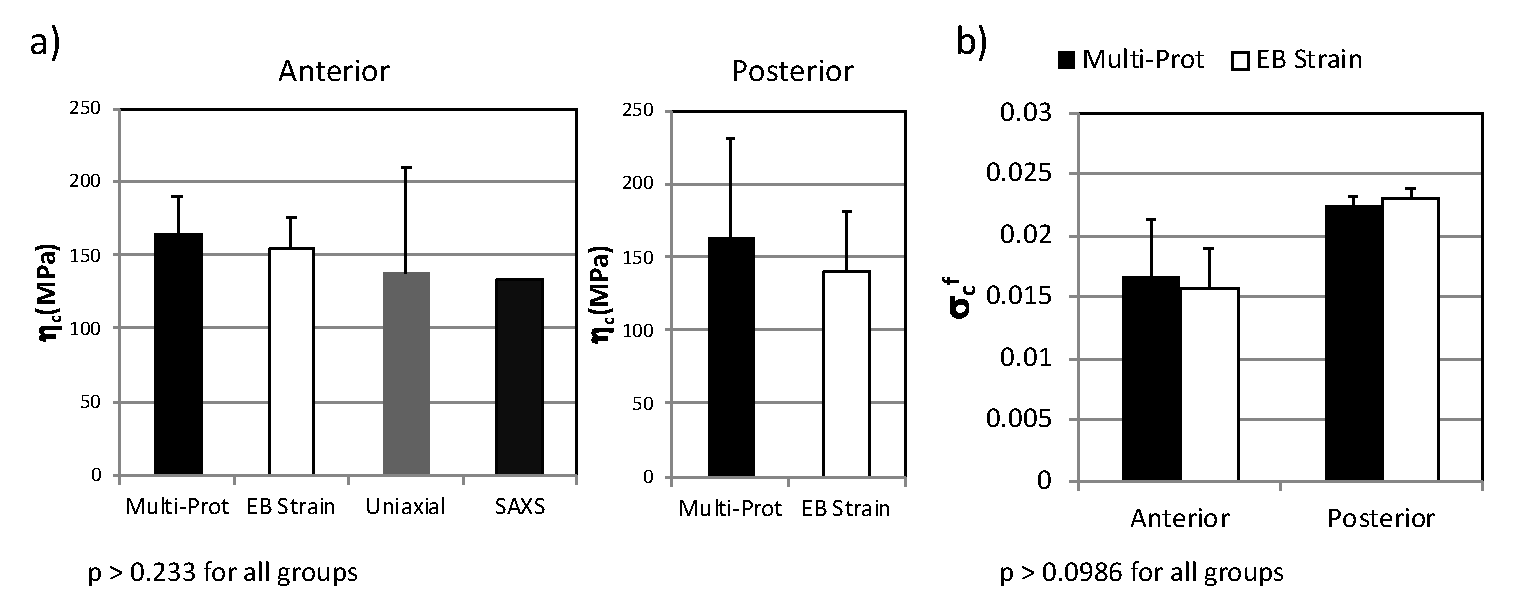
\includegraphics[width=\textwidth]{Images/chapter2/figure5.pdf}
\caption{(a) The mean and standard deviation of the collagen fiber modulus as determined from uniaxial, equibiaxial strain, and planar biaxial stress testing for both the anterior and posterior leaflets is shown. No statistical significant was found from ANOVA and student-t tests. (b) The mean and standard deviation of $\sigma_r$, which is standard deviation of the recruitment distribution of collagen fibers, in the fibrosa layer for both the anterior and posterior leaflet is shown. Again, no statistical significance was found, but the posterior leaflet appears to have larger $\sigma_r$ based on the trend.}
\label{c2:fig:5}
\end{figure}
%%%%%%%%%%%%%%%%%%%%	 end FIGURE 	%%%%%%%%%%%%%%%%%%%%


\begin{sidewaystable}
\centering
\caption{Parameter estimation results from the MV anterior leaflet.}\label{c2:tab:6}
\begin{tabular}{L{.5in}L{.55in}L{.4in}L{.4in}L{.4in}L{.4in}L{.4in}L{.4in}L{.4in}L{.4in}L{.4in}L{.4in}L{.4in}}
\hline
& \multicolumn{12}{c}{\textbf{Collagen}}    \\
\cline{2-13}
& \textbf{Modu.} & \multicolumn{4}{c}{\textbf{Fibrosa + Ventricularis}} & \multicolumn{4}{c}{\textbf{Atrialis}} & \multicolumn{3}{c}{\textbf{Spongiosa}}  \\
\hline
\textbf{ID} & $\mathbf{\eta}_c$ & $\sigma_c^f$ & $\mu_r^f$ & $\sigma_r^f$ & $E_{ub}^f$ & $\sigma_c^a$ & $\mu_r^a$ & $\sigma_r^a$ & $E_{ub}^a$ & $\mu_r^s$ & $\sigma_r^s$ & $E_{ub}^s$   \\
\hline
1 & 144.92 & 0.163 & 0.210 & 0.010 & 0.223 & 0.465 & 0.864 & 0.042 & 0.989 & 0.790 & 0.015 & 0.835  \\
2 & 86.23 & 0.140 & 0.522 & 0.010 & 0.537 & 0.077 & 1.172 & 0.019 & 1.204 & 1.177 & 0.038 & 1.256   \\
3 & 235.26 & 0.075 & 0.425 & 0.041 & 0.494 & 0.075 & 0.613 & 0.028 & 0.653 & 0.676 & 0.015 & 0.720  \\
4 & 199.33 & 0.136 & 0.293 & 0.011 & 0.307 & 0.075 & 0.914 & 0.010 & 0.927 & 0.890 & 0.010 & 0.902  \\
5 & 207.55 & 0.149 & 0.391 & 0.006 & 0.397 & 0.400 & 1.791 & 0.154 & 2.099 & 1.798 & 0.006 & 1.810  \\
6 & 196.41 & 0.180 & 0.286 & 0.015 & 0.307 & 0.250 & 0.520 & 0.019 & 0.545 & 0.525 & 0.015 & 0.559  \\
7 & 69.35 & 0.222 & 0.275 & 0.024 & 0.300 & 0.075 & 0.472 & 0.015 & 0.517 & 0.540 & 0.026 & 0.617   \\
Mean & 162.72 & 0.153 & 0.335 & 0.017 & 0.361 & 0.170 & 0.759 & 0.022 & 0.806 & 0.766 & 0.020 & 0.815   \\
SEM & 26.16 & 0.020 & 0.047 & 0.005 & 0.051 & 0.066 & 0.111 & 0.005 & 0.113 & 0.100 & 0.004 & 0.103 \\


\hline
& \multicolumn{8}{c}{\textbf{Elastin}} & & \textbf{Mat.} & \textbf{Ori.} & \textbf{$R^2$}  \\
\cline{2-13}
& \multicolumn{3}{c}{\textbf{Ventricularis}} & \multicolumn{3}{c}{\textbf{Atrialis}} & \multicolumn{2}{c}{\textbf{Spongiosa}} & & & &  \\
\hline
\textbf{ID} & $\mathbf{\eta}_e^v$ & $d^v$ & $\sigma_e^v$ & $\mathbf{\eta}_e^v$ & $d^v$ & $\sigma_e^v$ & $\mathbf{\eta}_e^v$ & $d^v$ & & $\mathbf{\eta}_m$ & $\mu_\theta$ &    \\
\hline
1 & 53.91 & 2.878 & 0.077 & 125.0 & 1.732 & 0.078 & 54.67 & 2.747 & & 0.000 & 0.304 & 0.980   \\
2 & 0.07 & 3.416 & 0.079 & 0.12 & 2.982 & 0.082 & 0.04 & 1.742 & & 0.010 & 0.350 & 0.893      \\
3 & 12.25 & 3.500 & 0.077 & 27.21 & 3.000 & 0.079 & 0.06 & 2.986 & & 0.000 & 0.622 & 0.957    \\
4 & 14.52 & 3.000 & 0.076 & 67.28 & 1.000 & 0.151 & 0.00 & 2.048 & & 0.000 & 0.384 & 0.986    \\
5 & 2.08 & 2.980 & 0.106 & 0.05 & 1.681 & 0.340 & 0.00 & 1.553 & & 0.911 & -0.05 & 0.970     \\
6 & 13.71 & 3.443 & 0.081 & 287.3 & 2.132 & 0.097 & 0.00 & 2.824 & & 0.281 & 0.449 & 0.996    \\
7 & 2.33 & 1.886 & 0.199 & 0.34 & 2.704 & 0.341 & 0.00 & 3.000 & & 0.000 & -0.20 & 0.970     \\
Mean & 16.13 & 3.021 & 0.098 & 84.55 & 2.258 & 0.138 & 9.13 & 2.558 & & 0.049 & 0.274 & 0.964 \\
SEM & 7.9 & 0.250 & 0.020 & 44.94 & 0.324 & 0.042 & 9.13 & 0.217 & & 0.047 & 0.102 & 0.015    \\
\hline
\end{tabular}
\end{sidewaystable}



\begin{sidewaystable}
\centering
\caption{Parameter estimation results from the MV Posterior leaflet.}\label{c2:tab:7}
\begin{tabular}{L{.5in}L{.55in}L{.4in}L{.4in}L{.4in}L{.4in}L{.4in}L{.4in}L{.4in}L{.4in}L{.4in}L{.4in}L{.4in}}
\hline
& \multicolumn{12}{c}{\textbf{Collagen}}    \\
\cline{2-13}
& \textbf{Modu.} & \multicolumn{4}{c}{\textbf{Fibrosa + Ventricularis}} & \multicolumn{4}{c}{\textbf{Atrialis}} & \multicolumn{3}{c}{\textbf{Spongiosa}}  \\
\hline
\textbf{ID} & $\mathbf{\eta}_c$ & $\sigma_c^f$ & $\mu_r^f$ & $\sigma_r^f$ & $E_{ub}^f$ & $\sigma_c^a$ & $\mu_r^a$ & $\sigma_r^a$ & $E_{ub}^a$ & $\mu_r^s$ & $\sigma_r^s$ & $E_{ub}^s$   \\
\hline
1 & 200.000 & 0.352 & 0.300 & 0.011 & 0.314 & 0.400 & 0.487 & 0.033 & 0.539 & 1.554 & 0.168 & 2.020 \\
2 & 197.276 & 0.247 & 0.393 & 0.010 & 0.411 & 0.400 & 0.840 & 0.051 & 0.966 & 1.911 & 0.157 & 2.218 \\
3 & 96.535 & 0.422 & 0.715 & 0.044 & 0.760 & 0.427 & 2.500 & 0.158 & 2.966 & 1.329 & 0.020 & 1.369  \\
4 & 160.354 & 0.216 & 0.543 & 0.010 & 0.558 & 0.400 & 1.323 & 0.052 & 1.436 & 2.028 & 0.018 & 2.079 \\
5 & 200.000 & 0.370 & 0.454 & 0.033 & 0.501 & 0.104 & 1.366 & 0.048 & 1.480 & 0.780 & 0.037 & 0.824 \\
6 & 181.100 & 0.292 & 0.608 & 0.017 & 0.639 & 0.400 & 1.380 & 0.079 & 1.563 & 1.079 & 0.039 & 1.196 \\
7 & 112.588 & 0.325 & 0.392 & 0.032 & 0.428 & 0.400 & 0.699 & 0.064 & 0.890 & 1.668 & 0.107 & 1.811 \\
Mean & 163.979 & 0.318 & 0.486 & 0.022 & 0.516 & 0.362 & 1.228 & 0.069 & 1.406 & 1.478 & 0.078 & 1.645  \\
SEM & 16.330 & 0.027 & 0.054 & 0.005 & 0.057 & 0.043 & 0.251 & 0.016 & 0.296 & 0.169 & 0.025 & 0.197    \\



\hline
& \multicolumn{8}{c}{\textbf{Elastin}} & & \textbf{Mat.} & \textbf{Ori.} & \textbf{$R^2$}  \\
\cline{2-13}
& \multicolumn{3}{c}{\textbf{Ventricularis}} & \multicolumn{3}{c}{\textbf{Atrialis}} & \multicolumn{2}{c}{\textbf{Spongiosa}} & & & &  \\
\hline
\textbf{ID} & $\mathbf{\eta}_e^v$ & $d^v$ & $\sigma_e^v$ & $\mathbf{\eta}_e^v$ & $d^v$ & $\sigma_e^v$ & $\mathbf{\eta}_e^v$ & $d^v$ & & $\mathbf{\eta}_m$ & $\mu_\theta$ &    \\
\hline
1 & 83.48 & 2.866 & 0.129 & 789.7 & 1.686 & 0.400 & 234.7 & 2.610 & & 0.001 & -0.60 & 0.993  \\
2 & 1.537 & 2.705 & 0.082 & 0.029 & 3.000 & 0.085 & 0.011 & 1.000 & & 0.000 & -0.04 & 0.967  \\
3 & 0.743 & 2.918 & 0.349 & 0.000 & 2.999 & 0.400 & 0.000 & 2.549 & & 0.000 & -0.31 & 0.864  \\
4 & 0.685 & 2.884 & 0.078 & 1.223 & 1.006 & 0.092 & 0.041 & 2.874 & & 0.000 & 1.425 & 0.930   \\
5 & 0.198 & 1.044 & 0.285 & 2.993 & 2.116 & 0.393 & 0.778 & 3.000 & & 0.426 & -0.39 & 0.972  \\
6 & 0.103 & 1.001 & 0.075 & 0.000 & 2.731 & 0.311 & 0.000 & 1.774 & & 0.253 & -0.23 & 0.984  \\
7 & 1.789 & 2.050 & 0.285 & 239.3 & 3.000 & 0.400 & 119.7 & 3.000 & & 0.333 & -0.16 & 0.985  \\
Mean & 12.65 & 2.210 & 0.183 & 147.6 & 2.363 & 0.297 & 50.74 & 2.401 & & 0.145 & -0.32 & 0.956   \\
SEM & 11.81 & 0.326 & 0.045 & 112.2 & 0.297 & 0.055 & 34.98 & 0.283 & & 0.071 & 0.170 & 0.017 \\
\hline
\end{tabular}
\end{sidewaystable}


    Next, we compared the result for the two collagen fiber recruitment models: orientation-invariant (Eqn. \ref{eqn:recruitmentasafunctionnormal}) and orientation-variant (Eqn. \ref{eqn:recruitmentasafunctionofangle}). Interestingly, we found no major difference between these modeling approaches (Fig. \ref{c2:fig:6}). The R-squared value of fit was very good for both models ($R^2$ = 0.996 vs 0.988 for Eqns. \ref{eqn:recruitmentasafunctionnormal}, \ref{eqn:recruitmentasafunctionofangle} respectively). There were no significant difference in the predicted collagen fiber modulus $\eta_c$ (Fig. \ref{c2:fig:6}a) and the collagen fiber $\Gamma(\theta)$ shows only a difference of $0.44^\circ$ in $\eta_c$ for the atrialis and $1.21^\circ$ in  for the fibrosa (Fig. \ref{c2:fig:6}b). Furthermore, the collagen fiber recruitment distribution $D(\mathbf{\xi}, x)$ when scaled to the same range [0,1] by their upper-bound value (Fig. \ref{c2:fig:6}c) were similar for either case.
    
    
%%%%%%%%%%%%%%%%%%%%	begin FIGURE 	%%%%%%%%%%%%%%%%%%%%
\begin{figure}
\centering
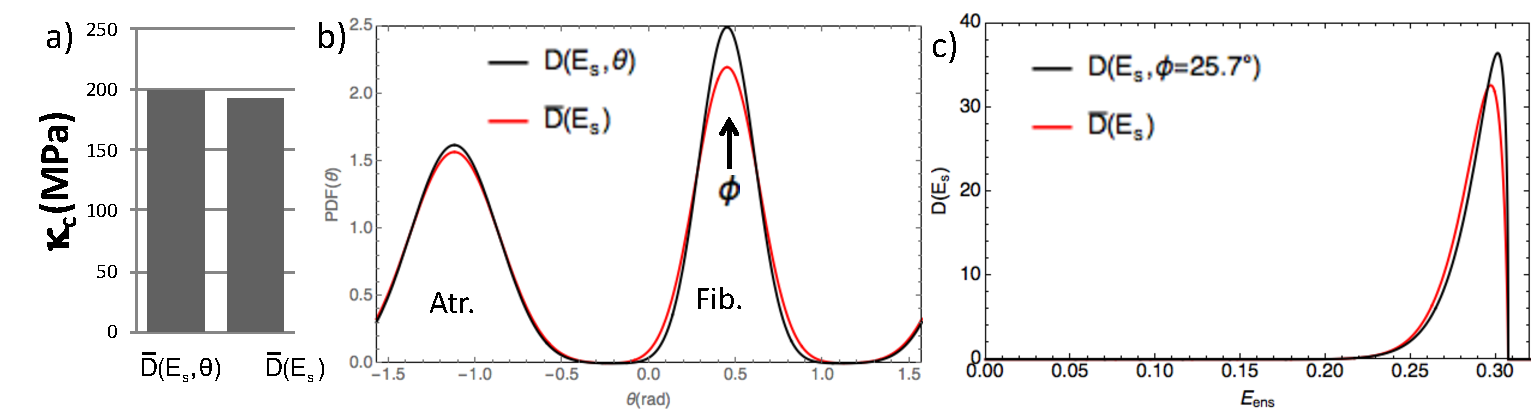
\includegraphics[width=\textwidth]{Images/chapter2/figure6.pdf}
\caption{The specimen was fit using both the comparisons for the orientation-variant $\bar{D}(\bar{\mathbf{\xi}},x)$ (Black) and orientation invariant $D(\mathbf{\xi},x,\mathbf{n}_0)$ (Red) modeling approaches for the recruitment functions. Both methods produce (a) nearly the same collagen fiber modulus. (b) The fiber ODFs also appears to the equivalent width ($\sigma_c^f$). (c) The recruitment distribution also appears to be similar.}
\label{c2:fig:6}
\end{figure}
%%%%%%%%%%%%%%%%%%%%	 end FIGURE 	%%%%%%%%%%%%%%%%%%%%
    
    
    The optimal recruitment parameters for both the multi-protocol data and the EB strain data were very similar (Table \ref{c2:tab:5}, \ref{c2:tab:6}, \ref{c2:tab:7}). We found no significant differences in the averaged standard deviation of recruitment, $\sigma_r$, between the anterior and posterior leaflets for either tests (Fig. \ref{c2:fig:5}b). There were minor differences in the distributions due to the way the upper-bound parameter was determined. The analysis of the EB strain kinematic state was done visually, where the upper-bound may have been underestimated. For analysis of the stress controlled planar biaxial tests, which does not reach full recruitment, the upper-bound was predicted by the parameter estimation algorithm and tended to be slightly overestimated. Uniaxial testing instead shows a very different recruitment response (Table \ref{c2:tab:4}). This is most likely due to the vastly different testing modes, where the differences in preconditioning and gauge length result in a drastically different reference state for the fibers. Additionally, fiber rotation effects in the uniaxial testing slow the recruitment of fibers away from the test axis and produce a greater standard deviation for the recruitment distribution. We however observe in trend that the posterior leaflet recruits slower than the anterior leaflet (Fig. \ref{c2:fig:5}b), possibly due to differences in their role mechanically during valve closure.
    
    


\subsection{Parameter validation} \label{c2:sec:233}

    Perhaps the most important validation finding was that the simulated SAXS response (Eqn. \ref{c2:eqn:fibrilstrain}), using the best fit parameters, matched very well to the MV SAXS data from Liao et al. \cite{liao_relation_2007} (Fig. \ref{c2:fig:7}). The squared correlation coefficient was computed ($r^2 = 0.971$), and we found no statistical significance ($p = 0.285$) between the two curves. To assess the sensitivity of the SAXS simulation (Eqn. \ref{c2:eqn:fibrilstrain}), the origin recruitment distribution parameters $\mu_r^f = 0.286$ and $E_{ub}^f = 0.307 $ were shifted by $\pm0.01$ in Green Lagrange strain, and the standard deviation of the collagen fiber ODF $\sigma_r^f = 10.3^\circ (\Gamma_c(\theta))$ was adjusted by $\pm1^\circ$ (Fig. \ref{c2:fig:7}). Despite the perturbation being so small, there was a 54\% increase in the slope of the simulated SAXS response when the mean and upper-bound of the recruitment was increased by 0.01, and a 38\% decrease in slope when the parameters were decreased by 0.01. Similarly, the slope decreased by 17\% when  was increased by $1^\circ$, and increased by 20\% when decreased by $1^\circ$. 
    An estimate of the fiber modulus for the MV SAXS data was made by comparing against the simulated data. No statistical significance for the collagen fiber modulus between any mechanical tests or between either leaflets was found. In addition, the predicted ODFs $\Gamma_c(\theta)$ and $\Gamma_e(\theta)$ compared very well with the SHG measurements, with standard deviations differing by no more than 3 degrees (Fig. \ref{c2:fig:8}). Thus, despite the model complexity, these validation results suggest that the parameters were sufficiently independent and each can be accurately determined as a representation of the mechanical behavior of the MV.
    
    
%%%%%%%%%%%%%%%%%%%%	begin FIGURE 	%%%%%%%%%%%%%%%%%%%%
\begin{figure}
\centering
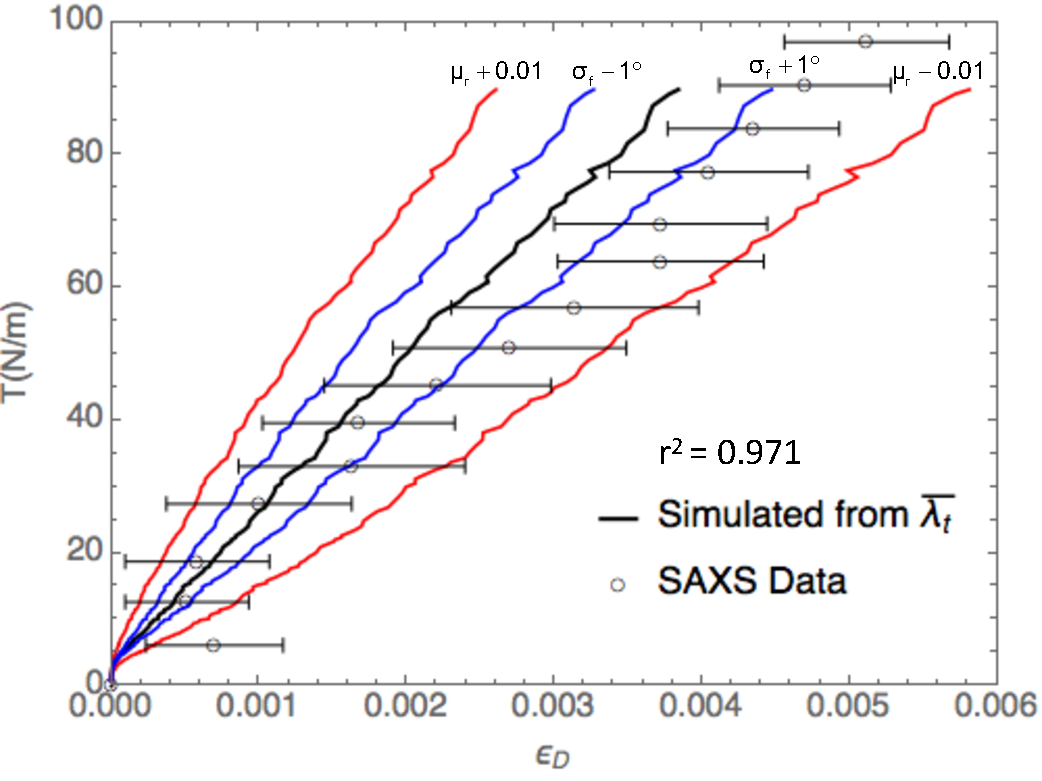
\includegraphics[width=0.75\textwidth]{Images/chapter2/figure7.pdf}
\caption{Collagen fibril stress–strain data from SAXS studies from Liao et al. \cite{liao_relation_2007} (circles) along with the simulated result based on the current model parameters (Black) showing very good agreement. This approach is very sensitive. Perturbing the ODF ($\sigma_c^f$) by $1^\circ$ (Blue) and shifting the recruitment distribution by 0.01 in Green strain (Red) significantly changed the slop of the curve.}
\label{c2:fig:7}
\end{figure}
%%%%%%%%%%%%%%%%%%%%	 end FIGURE 	%%%%%%%%%%%%%%%%%%%%


%%%%%%%%%%%%%%%%%%%%	begin FIGURE 	%%%%%%%%%%%%%%%%%%%%
\begin{figure}
\centering
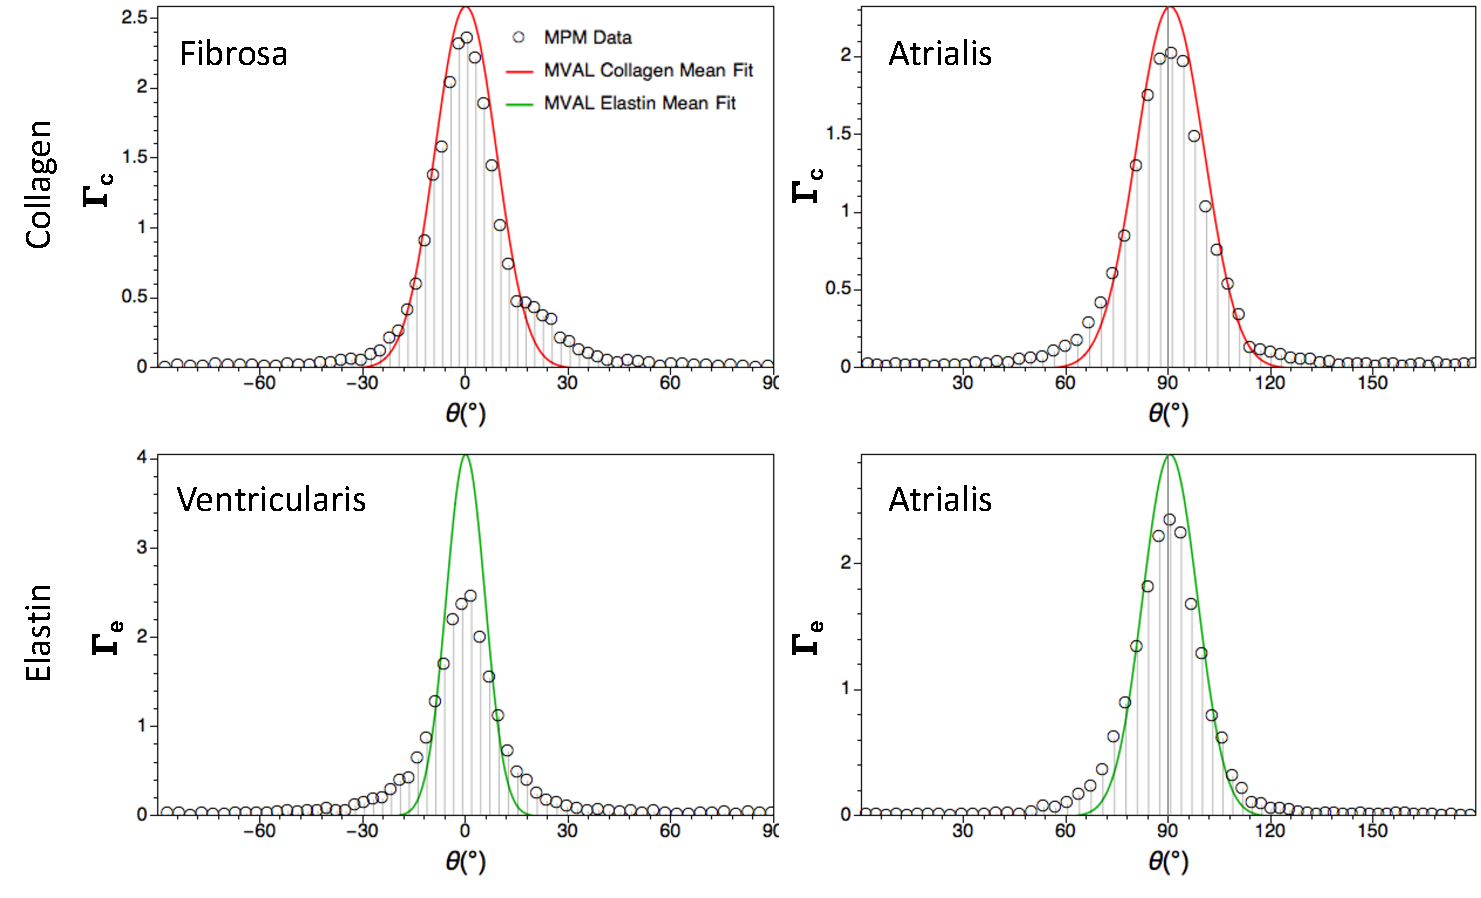
\includegraphics[width=\textwidth]{Images/chapter2/figure8.pdf}
\caption{The fitted orientation distribution functions of the collagen (Red) and elastin (Green) for the anterior leaflet are shown in comparison to the measured distribution from SHG (circle). The results are shown for the ventricularis, fibrosa and atrialis. The fitted and measured ODF appears to show good agreement. }
\label{c2:fig:8}
\end{figure}
%%%%%%%%%%%%%%%%%%%%	 end FIGURE 	%%%%%%%%%%%%%%%%%%%%




\subsection{Differences between layers and leaflets}

    All ODFs $\Gamma(\theta)$ of the ventricularis, fibrosa and atrialis were much narrower in the anterior leaflets than the posterior leaflets (Fig. \ref{c2:fig:9}). To estimate the mean ensemble elastin response, each elastin ensemble was scaled by the principle strain at maximum loading under EB stress and then averaged. Like the structural differences between the anterior and posterior leaflets, the mechanical response of ventricularis was much stiffer in the anterior leaflets comparing to the posterior leaflet (Fig. \ref{c2:fig:10}). On the other hand, the atrialis was stiffer in the posterior leaflet (Fig. \ref{c2:fig:10}). For the overall layer contributions, the mechanical response of the circumferential direction is mainly due to the elastin in the ventricularis at lower stress and the collagen within the fibrosa at high stress, whereas the radial direction is a combination of collagen fibers in the fibrosa as they extend and rotate under physiological loading and collagen in the atrialis at higher strains (Fig. \ref{c2:fig:11}). The mechanical contribution from the spongiosa was, as anticipated, negligible for both leaflets.
    
    
%%%%%%%%%%%%%%%%%%%%	begin FIGURE 	%%%%%%%%%%%%%%%%%%%%
\begin{figure}
\centering
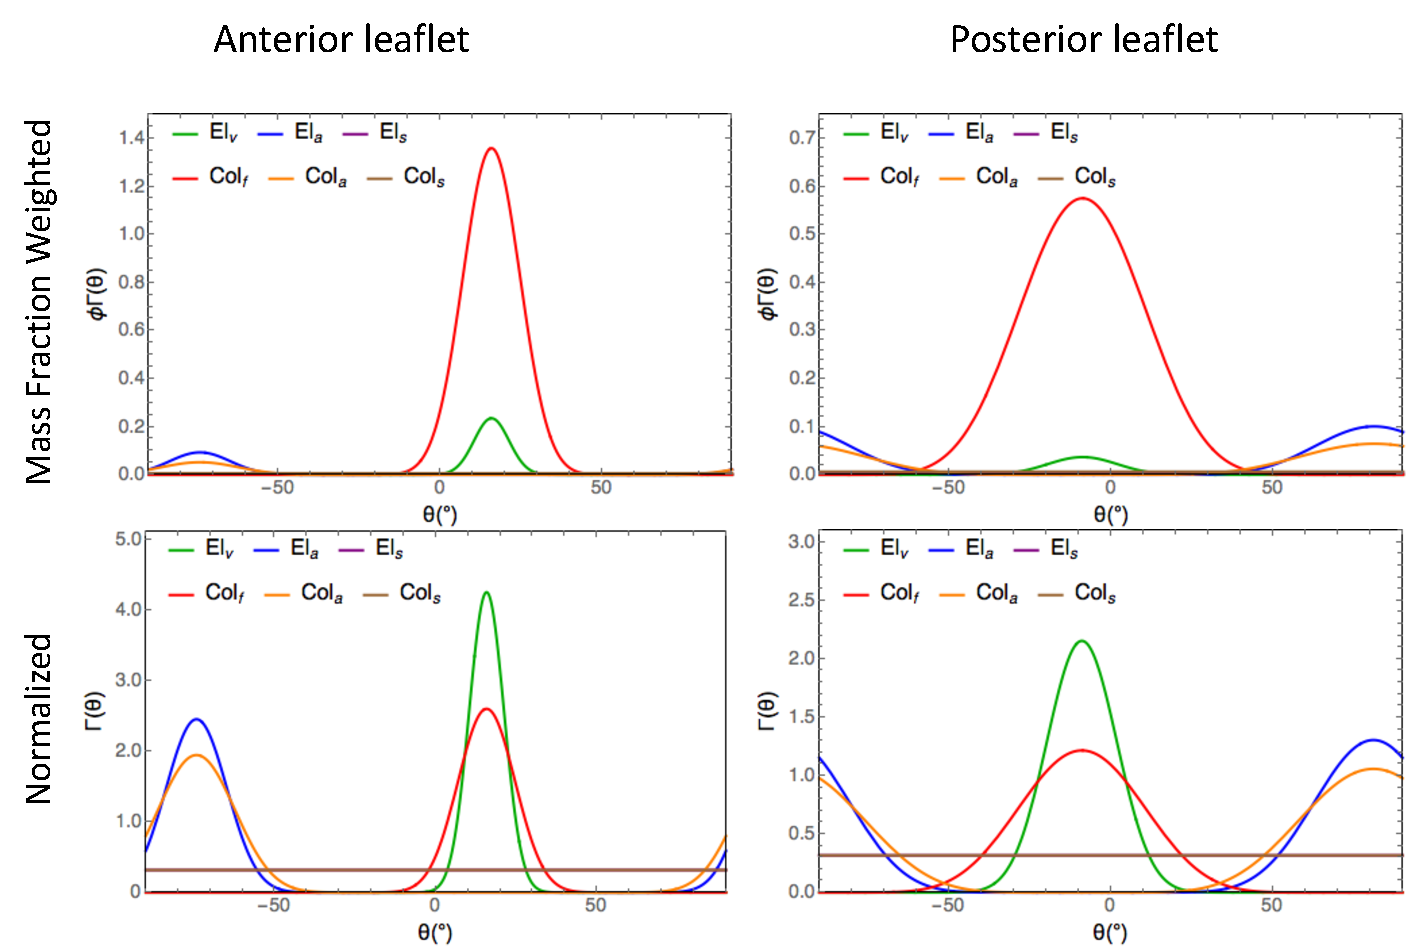
\includegraphics[width=\textwidth]{Images/chapter2/figure9.pdf}
\caption{The predicted fiber orientation distributions from the anterior (Left) and posterior leaflets (Right) for collagen and elastin from all layers as an average (n = 7 for both leaflets). Both the mass fraction scaled (Top) and normalized (Both) ODFs are shown. In both leaflets the collagen of the fibrosa layer is clearly the most dominant, but is more broadly distributed in the posterior leaflet. Elastin is also similarly trends but is more evenly distributed in the anterior leaflet, while favoring the atrialis in the posterior leaflet.}
\label{c2:fig:9}
\end{figure}
%%%%%%%%%%%%%%%%%%%%	 end FIGURE 	%%%%%%%%%%%%%%%%%%%%


%%%%%%%%%%%%%%%%%%%%	begin FIGURE 	%%%%%%%%%%%%%%%%%%%%
\begin{figure}
\centering
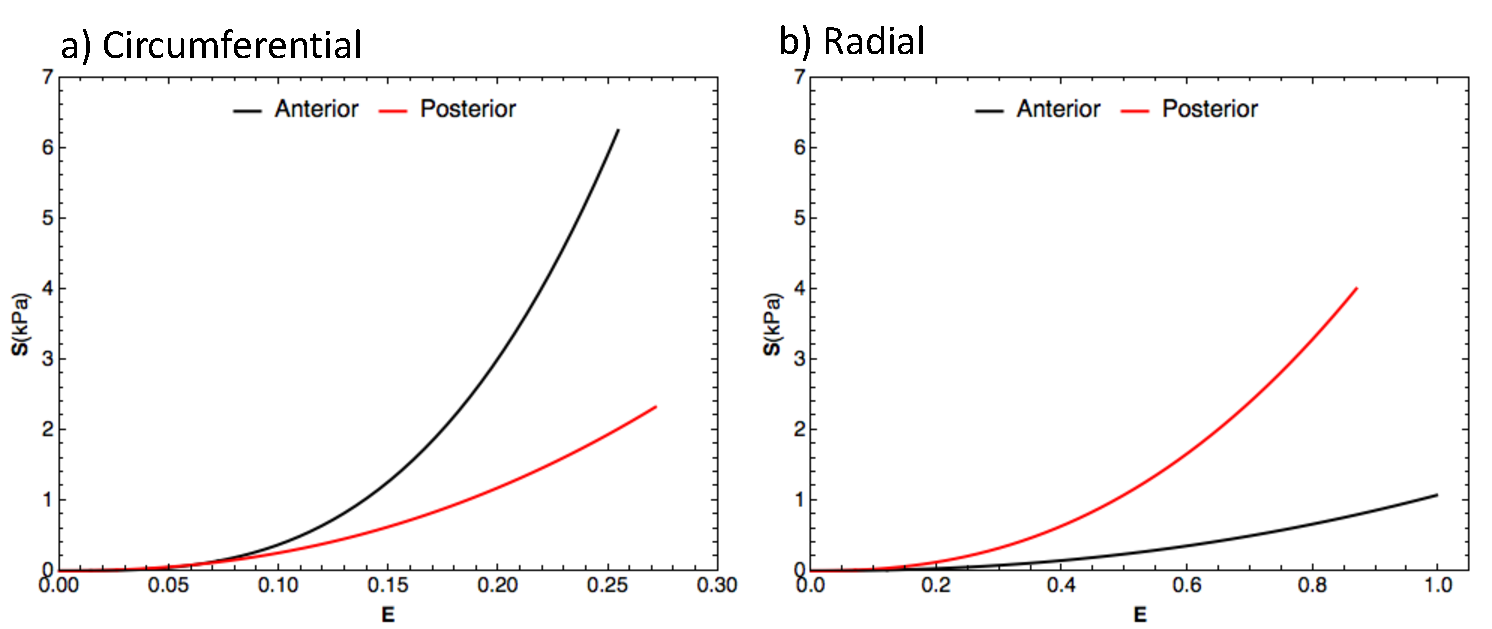
\includegraphics[width=\textwidth]{Images/chapter2/figure10.pdf}
\caption{The mean elastin response in the physiological range from both anterior (Black) and posterior (Red) leaflets in the circumferential (a) and radial (b) directions. n = 7 for both leaflets. The elastin in the anterior leaflet is heavily anisotropy and favoring the circumferential direction, which the elastin in the posterior leaflet is more isotropic and only slightly favoring the radial direction.}
\label{c2:fig:10}
\end{figure}
%%%%%%%%%%%%%%%%%%%%	 end FIGURE 	%%%%%%%%%%%%%%%%%%%%


%%%%%%%%%%%%%%%%%%%%	begin FIGURE 	%%%%%%%%%%%%%%%%%%%%
\begin{figure}
\centering
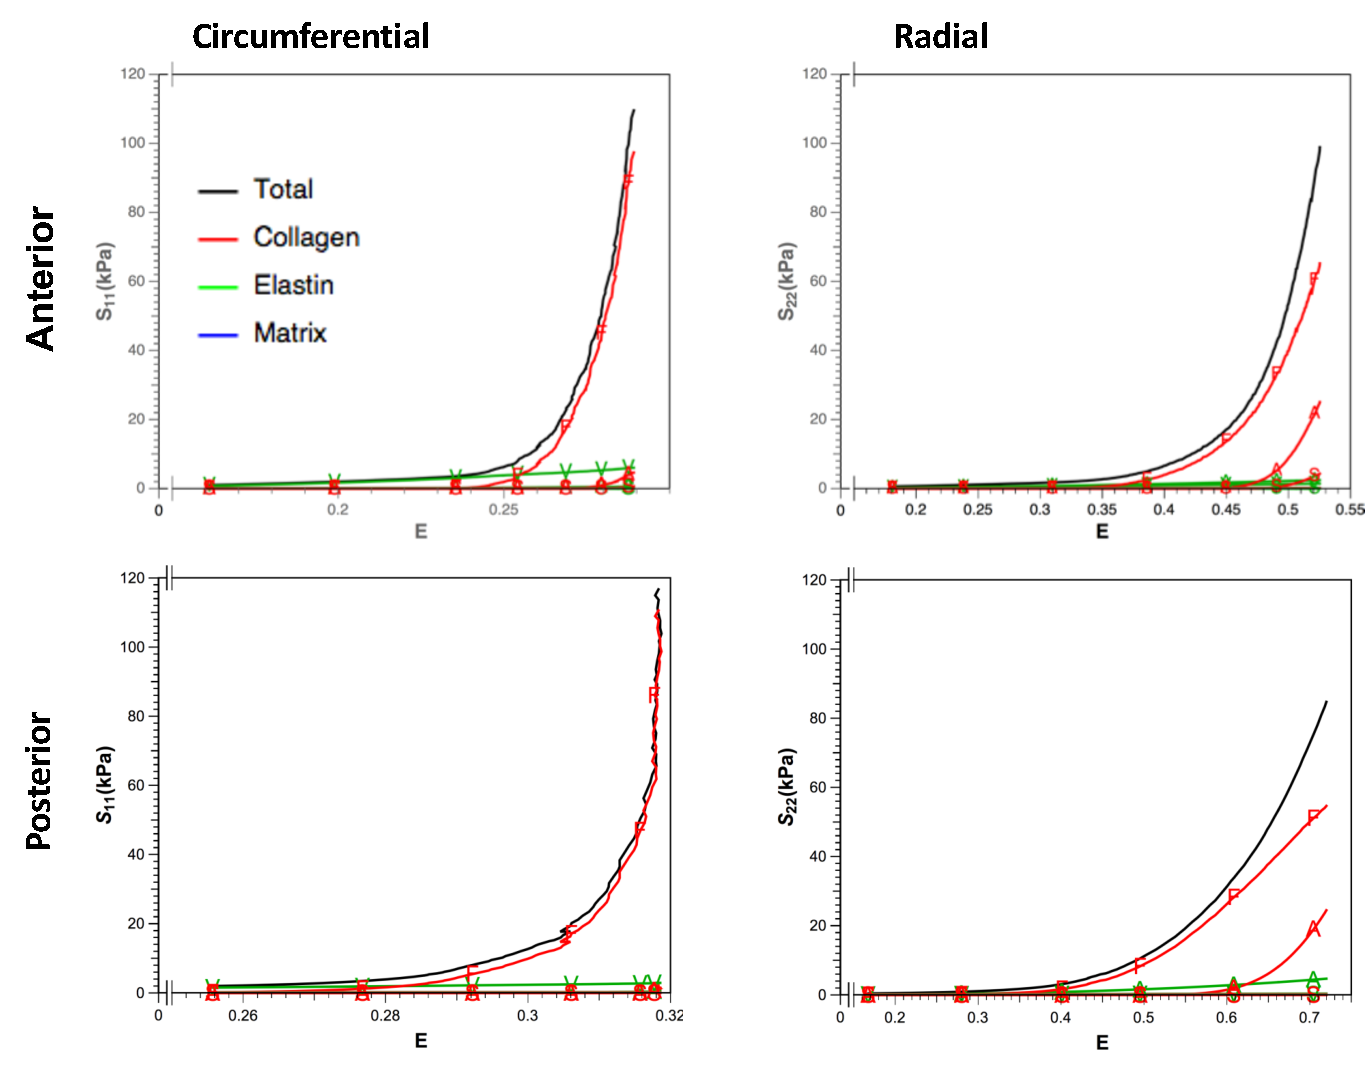
\includegraphics[width=\textwidth]{Images/chapter2/figure11.pdf}
\caption{The net stress contribution from each ECM component from each layer for the equibiaxial stress protocol is shown for the circumferential (Left) and radial (Right) direction of the anterior (Top) and posterior (Bottom) leaflets. Here, the contributions from the layers are ventricularis (V), fibrosa (F), spongiosa (S), and atrialis (A). Interestingly, while the fibrosa layer is dominant circumferential directions in both leaflets, the atrialis also contributes substantially in the radial direction. Elastin clearly contributes minimal stress comparing to collagen, but it forms the bulk of the response in the toe region.}
\label{c2:fig:11}
\end{figure}
%%%%%%%%%%%%%%%%%%%%	 end FIGURE 	%%%%%%%%%%%%%%%%%%%%






%---    Discussion
\section{Discussion}

\subsection{Modeling approach and major findings}

    In the present study, we developed a novel layer-specific meso-scale structural model of the MV leaflets starting from the fiber-level. The mechanical response at the layer- and tissue-level is driven by structural measurements and observations obtained from SHG and histology. We then utilized an extensive experimental mechanical database that included uniaxial, planar EB strain, and a comprehensive set planar biaxial stress test protocols. This approach allowed us to properly evaluate the mechanical properties of MV tissues and to form a complete dataset for parameter estimation. All information was then integrated to form a predictive model for the MV leaflet tissues.
    
    
\subsection{Model validation}

    Novel to this study was the use of the MV SAXS data \cite{liao_relation_2007} to validate the predicted collagen fiber modulus and fiber recruitment (Section \ref{c2:sec:26}). SALS techniques have been previously used to obtain the orientation of fibrous structures in biological tissues \cite{sacks_small_1997}. However, the wavelength of light (in the hundreds of nm) is much too large in comparison the size of the fibrils, which have a D-period of approximately 64 nm \cite{kastelic_structural_1980,hodge_recent_1963,chapman_electron_1984}. SAXS, on the other hand, utilizes a wavelength of 0.1–0.2 nm, and provides a direct way of measuring the collagen fibril D-period, and thus the fibril strains \cite{sasaki_elongation_1996,sasaki_stress_1996,liao_relation_2007}. In response to tissue-level deformation, the fibril strain depends on both its orientation and slack strain (Section \ref{c2:sec:26}). Therefore, the MV SAXS simulation can provide an independent way of validating the MSSCM collagen model component. Both the good agreement and sensitivity to accurate measures (Section \ref{c2:sec:233}, Fig. \ref{c2:fig:7}) provides additional confidence in our approach beyond basic measures such as goodness of fit. In particular, this lends confidence to the fiber/fibril kinematics used in the present form of the MSSCM, and suggests that the fibrils do indeed form contiguous, tightly bounded fibers and undergo minimal slipping.
    
    
    It is also important to note that it is difficult to directly combine measurements at multiple scales, such as fibril strain as measured by SAXS and the applied tissue-level membrane stress, and interpret them directly. In this case, we cannot approximate the modulus of collagen fibrils using the slope of the tissue-level stress–fibril strain curve. Although we assume every fibril has a similar modulus, the apparent modulus of collagen fibrils at the tissue-level decreases in response to increase in the slack stretch (Eqn. \ref{eqn:collagenfiberlaw}). Thus interpretation of such results requires careful analysis of the structure and kinematically related mechanisms of the tissue. Finally, we also validated the fiber $\Gamma(\theta)$ against optical SHG measurements, which demonstrated very good agreement (Fig. \ref{c2:fig:8}). To the authors’ knowledge, this is the first time macro/micro validations of this kind have been performed for any soft tissue
    
    


\subsection{Collagen fiber modulus}

    As the most important load bearing component of soft tissues, the structure and properties of collagen is of major interest. One specific property is the modulus of the collagen fiber, which when combined with the level of fiber undulation, determines the macroscopic behavior of the collagen network at the tissue-level. Given that type I collagen fibers forms the common building blocks for the bulk of the MV tissue (Fig. \ref{c2:fig:2}), the modulus serves both as an important validation for the results of the model and predicting the correct behavior of the tissue under complex loading conditions. There have been many attempts to measure the stiffness of collagen fibers in the literature \cite{shen_stress_2008,gentleman_mechanical_2003,eppell_nano_2006,yang_mechanical_2008,yang_micromechanical_2007,wenger_mechanical_2007}. These measurements come in two forms: (1) models at the tissue-level and (2) direct measurements at the fibril-level. Measurements at the tissue-level can be inaccurate, as they demand an extensive understanding of biomechanics of the tissue, physically accurate models of the mechanical behavior and detailed measurements of the structure and composition. On the other hand, there is currently no method for the real time estimation of the instantaneous cross sectional area of collagen fiber or fibrils. Current measurements are typically done a priori \cite{gentleman_mechanical_2003} or a posteriori \cite{eppell_nano_2006}, and can have significant impact on the results. These measurements also require highly accurate and noise insensitive instruments operating at the micrometer and nanometer scale. As such, these experiments are typically done using techniques such as atomic force microscopy (AFM) and have a large variability for the resulting numbers. Nonetheless, these measurements serve as an important reference for any results measure at the tissue-level, and the current literature paints a distinct picture.


    For the most part, these findings fall into two distinct categories: (1) the dried properties at the 2–10 GPa range and (2) hydrated properties at the 200–900 MPa range. This difference in stiffness is due to water acting as a plasticizer in collagen fibrils [62]. Using AFM, Yang et al. \cite{yang_micromechanical_2007} found a stiffness of 1.4 GPa for non-cross linked fibrils and 3.4 GPa for cross-linked collagen fibrils in the bovine Achilles tendon. Similarly, Wenger et al. \cite{wenger_mechanical_2007} found collagen fibril stiffness of 5–11.5 GPa in rat tail tendon. However, in both papers the fibrils were dried under ambient conditions and nitrogen, respectively. On the other side, Shen et al. \cite{shen_stress_2008} found a modulus of $860\pm450$ MPa for collagen fibrils obtained from sea cucumber dermis. In the study by Gentleman et al. [23], they found a modulus of $269.7\pm11.9$ to $484.7\pm76.3$ MPa for collagen fibers in the bovine Achilles tendon, varying with the fiber diameter, but only for the cross-linked fibers. Eppell et al. \cite{eppell_nano_2006}, found a modulus of 0.5–0.4 GPa at low strain (0.05–0.30) but can increase to up to 12 GPa at high strain. In these cases, the fibrils were hydrated before testing. This effect has also been studied using electrospun collagen scaffolds, where Yang et al. found that the fibril modulus decrease from 1.3–7.8 GPa to 0.07–0.26 GPa when hydrated\cite{yang_mechanical_2008}.


    In present study we found the collagen fiber modulus to be between 132.5 and 167.3 MPa. In our estimation of the collagen volume fraction, we assumed the tissue is entirely composed of collagen, elastin and proteoglycans. While this serves as a good estimation of the relative composition of the MV, fluid constitutes 81.8\% of the total mass of the MV anterior leaflet \cite{lis_biochemical_1987}. Additionally, using the dry mass is not a viable alternative as the fibers may have shrunk when they are dried \cite{leikin_raman_1997}. As such, we chose the current approach to provide an unbiased effective collagen modulus for the MV. This value is not applicable to other tissues with significantly different structural composition and may explain minor differences in the modulus estimate for the anterior and posterior leaflet. When the residual volume is taken into account, it is not difficult to imagine the estimated modulus to be 2–4 times higher than the value reported, allowing it to fall in line with the modulus of the hydrated collagen fibrils in other studies. This suggests that the model is reasonably accurate in estimating the mechanical properties of the collagen fibers. Furthermore, there were no statistical significance between the fiber modulus for either leaflet, which is reasonable given that the majority of collagen fibers are type I. Finally, that the assumption of minimal fiber–fiber and fiber–matrix interaction appears to be essentially correct. This is consistent with the ability for the fibers to rotate and extend freely with applied forces, keeping the effective tissue modulus low so the leaflets can coapt as necessary for valve function.
    
    
    
    
\subsection{Collagen fiber recruitment}

    While type I collagen naturally occurs in a crimped state, the bending stiffness as the collagen fiber unravels is typically small enough to allow us to use the recruitment approach \cite{lanir_constitutive_1983,fata_insights_2014,sacks_incorporation_2003,lanir_structural_1979,kastelic_structural_1980,hansen_recruitment_2002,cacho_constitutive_2007,grytz_constitutive_2009}. Novel to recruitment approach, we propose an angle variant recruitment distribution based on the hypothesis that the ensemble stress will be limited to a small range due to homeostasis. Current experimental techniques do not easily allow for direct measurement, and distinguishing individual fibers is difficult and sometimes required to be specified manually \cite{hill_theoretical_2012}. Determining whether a fiber is straightened is also problematic. For best accuracy, the fiber must lay in the plane of the image. The planar projection of a fiber at an angle with the plane of the image creates a misrepresentation of the tortuosity of the fiber. Additionally, the tissue must be loaded under EB strain with no shearing. Failure to do so will result in different strain for each fiber ensemble, thus the tortuosity of fibers at different angle cannot be referenced to the same strain. These issues are further magnified when quantifying angular variations. In the end, direct measurement methods are best served as a preliminary estimate for modeling purposes.


    Assuming that the ensemble stress of collagen fibers is constant with orientation due to homeostasis, both the current model (Eqn. \ref{eqn:recruitmentasafunctionofangle}) and the orientation-variant model (Eqn. \ref{eqn:recruitmentasafunctionnormal}) produce similar results for the MV leaflets; the quality of the best fits ($R^2 = 0.988$ vs $0.996$) are very comparable for both models. We hypothesize that this is due to the narrow splay of the collagen fiber ODF in the MV and thus the ensemble stress was effectively constant over this range for both models. This simplifies the recruitment distribution function for implementation in MV simulation and measurement via experimental means. Also, by assuming orientation-variance in Eqn. \ref{eqn:recruitmentasafunctionofangle}, the parameters are expressed as a percentage of the maximum ensemble strain, which is not an intuitive quantity. Thus, the parameters determined from Eqn. \ref{eqn:recruitmentasafunctionofangle} are best served as an approximation, rather than any physically accurate quantity. Therefore, we refocused the results as if the recruitment strains are invariant with angle (Eqn. \ref{eqn:recruitmentasafunctionnormal}), which has a more interpretive physical meaning. In either case, the theory then dictates that the tissue should exhibit a linear response once all fibers are straightened under EB strain loading. Indeed, this is observed in the MV for both the anterior (Fig. \ref{c2:fig:3}) and posterior leaflet.


    For each leaflet tested under EB strain and uniaxial extension, the stress strain curve transitions to linear in P–F \cite{sasaki_elongation_1996,sasaki_stress_1996,liao_relation_2007}. For the anterior leaflet this transition point occurs at $782.1\pm121.5$ kPa in 2nd Piola Kirchhoff or $1243.8\pm220.8$ kPa in Cauchy stress. Our inverse model using a full collagen mapped transverse model shows that the peak circumferential stress is at $241.4\pm40.5$ kPa and the peak radial stress is at $432.6\pm46.5$ kPa \cite{lee_inverse_2014}. While it is not possible to produce the equivalent ensemble stress for the in vivo data, it is estimated that only 20–40\% of fibers are recruited under physiological stress. This substantial structural reserve is likely an adaption to maintain structural integrity for when the body is under extraneous physiological stress or attempt to maintain basic function in cases of heart diseases.
    



\subsection{Elastin fiber network response}

    There is no established constitutive model form for individual elastin fibers in valvular tissue. We have taken a similar approach to modeling the fiber ensembles in the ovine pulmonary arteries \cite{fata_insights_2014}. However, in the MV, we noticed a slight nonlinearity in the pre collagen fiber recruitment response contrary to that of the pulmonary arteries \cite{fata_insights_2014}. It is not clear what the reason behind this is. Likely the cross-linking, both between and within a fiber in the elastin network, is different in order to fulfill the different functions for each tissue. To fit the low stress region, an exponential or power law is necessary. We chose the power law so we can constrain the order of the nonlinearity. This may result in some error when predicting and extrapolating past the range of the data. However, the stress contribution of elastin peaks at around 5–15 kPa at maximum stretch, which is much less that of the collagen (Fig. \ref{c2:fig:4}a), so this should not be a significant effect. The collagen also essentially functions as a stopper, putting a constraint on the maximum extension of the leaflets (especially in the circumferential direction). For this reason, the material model of the elastin this should not be a problem for the predictive capabilities of the model in most applications.


    Another interesting result is that the exponents of the elastin model differed between the layers and between the leaflets. This may be evidence of residual stress or strain between the layers. For the aortic valve, Stella and Sacks \cite{stella_biaxial_2007} noted that the elastin dominant ventricularis of the leaflet contracted by 10.9\% and 8.2\% in the radial and circumferential direction while the collagen dominant fibrosa elongated by 28.2\% and 4.8\% in the radial and circumferential direction after layer separation. Similar effect likely exists in the MV and the additional strain will result in a higher apparent stiffness due to the nonlinearity in the stress strain response. Thus the difference in the atrialis and ventricular of each leaflet may, at least in part, be due to this reason. It is interesting that the elastin in the anterior leaflet is significantly stiffer in the circumferential direction compared to that of the posterior leaflet, while in the radial direction it was the opposite. This corroborates with physical observations where the ventricularis in the posterior leaflet was much smaller compared to the anterior leaflet; sometimes nearly nonexistent. Again, this may be a product of the motion of the leaflets when closing.
    
    
    
    
\subsection{Layer structure and function}

    In the MV, the anterior leaflet extends to meet the posterior leaflet, while the posterior expands much less in comparison \cite{amini_vivo_2012,rausch_vivo_2011}. In order to accomplish this, the radial direction of the anterior leaflet needs to be able to extend significantly, while the circumferential direction needs to be able to maintain its integrity as it meets the posterior leaflet. There are a number of ways in which collagenous tissue have adapted to increase extensibility. The most common way is through adjustment in the crimping of the collagen fibers. However, once fiber recruitment is initiated, the tangent modulus increases rapidly, limiting further extension. A second method is through the rotation of fiber ensembles. As the ratio of radial to circumferential stretch increases, this induces a rotation of all fibers toward the radial direction. The overall effect is similar to recruitment due to crimping, but the tangent modulus increases more gradually in comparison. Intriguingly, this adaptation is seen in the MV leaflets. For both leaflets, collagen is mostly present in the fibrosa (Fig. \ref{c2:fig:2}). This results in the majority of collagen fibers being circumferentially aligned. Rather than having independent family of fibers each dictating the mechanical response of each direction, this is highly coupled (Fig. \ref{c2:fig:11}), with the bulk of the stress in the radial direction coming from the circumferential splay. However, the collagen fibers in atrialis are still needed for additional support. This makes the width of the fibers splay dictate the resulting response. In the anterior leaflet, the elastin and collagen fiber splays are narrower (Fig. \ref{c2:fig:9}), thus increasing the radial extensibility. Comparatively, the wider splay in the posterior leaflet produce a slightly more isotropic response resulting in smaller radial extension. Additionally, collagen fibers are also recruited faster in the anterior leaflet to further constrain the circumferential extension. Overall, collagen primarily functions to limit extension, whereas elastin determines the motion of the valve in the low stress region. This is perhaps why the radial direction of the anterior leaflet has the lowest stiffness, which allows for the fastest rate of extension. Interestingly, elastin is also the stiffest in circumferential direction of the anterior leaflet, following a similar trend as the collagen. The elastin in the posterior leaflet is likewise more isotropic than that of the anterior.
    
    
    
    
\subsection{Model predictive capabilities}

    Overall the model demonstrated very good ability to predict the extraphysiological protocols (Fig. \ref{c2:fig:4}c \& d). Using the correct mass fractions, for the ratio of collagen in the fibrosa vs the atrialis in particular, was especially important for accurately predicting these extra-physiological protocols. For predictive purposes, more leeway can be given for the mass fraction of elastin. Since the layers are treated completely independent of each other (not sharing a single modulus), errors in the mass fraction is absorbed by the modulus.
    
    
    
    
\subsection{Limitations}

    While every effort was made to ensure tissue viability, all studies were performed under in vitro conditions. While there appears to be differences between the in vivo properties of MV anterior leaflet \cite{krishnamurthy_material_2008} and the passive properties measured in an in vitro setting \cite{grashow_planar_2006,may-newman_biaxial_1995}. The mechanism behind these estimated differences remain unknown. It is unlikely to be due to the contractile forces exerted by the MV interstitial cells on the surrounding ECM, which appears to be small \cite{buchanan_interlayer_2013}. Residual stress may be involved, as studies have shown that the MV leaflets are also under significant residual strain \cite{amini_vivo_2012}. Additionally, the viscoelastic properties of the MV were not considered in this model, however we have found that the leaflet tissues are essentially functionally elastic \cite{grashow_biaxial_2006,grashow_planar_2006}. Direct validation of the individual layer stress contributions is not currently available, as it requires the separation of the individual layers, which in itself is a complex task. Additionally, a more sophisticated model is also necessary to take into account the effect of residual strain on the mechanical response. Nevertheless, we have shown that our models have good predictive capabilities for the mechanical response and fiber orientations distributions, and are validated using SAXS studies. Overall, this model is a faithful representation of the structural function relationship of MV tissues.

%---    Conclusion
\section{Conclusions and future directions}

In this study, we developed a novel fiber- and layer-specific structurally-driven constitutive model of the MV leaflets. The model incorporated fiber ODFs for collagen and elastin, collagen fiber recruitment, and related fiber-level mechanical phenomena. The model was validated by simulating the SAXS experiments and compared against the measured response. The results were consistent and show that the model correctly predicted the collagen fibril deformations measured by SAXS. Furthermore, the material parameters estimated were also consistent under EB strain testing and uniaxial testing. Thus the model is validated both via microscopic and meso-scale measurement. For the MV leaflets, we determined an effective modulus of 132.5–167.3 MPa for the collagen fibers which matches well with existing literature. This result suggests the tissue structure is an important predictor of leaflet function, where the fiber ODF and recruitment couples to determine the mechanical response of each leaflet. Moreover, fiber ODF tends to be narrower and the recruitment tends to happen over a smaller strain range to allow for a larger extension of the anterior leaflets while maintaining tensile strength. Overall, the model shows very good predictive ability and hopes to help in producing more accurate simulations of MV behavior in vivo, with the ultimate goal in improving long-term durability of MV repair.

This model may also serve as a baseline for the study of disease and aging valvular tissues. Pathological change to biological tissue is a very complex topic. In addition to the variety of pathological conditions, the changes due to a common disorder will be different among individuals. There is not yet sufficient data to fully understand and predict the mechanical changes. However, this model can serve as a starting point for analyzing the underlying changes due to pathological conditions, when the requisite data become available.

We should note that the utility of the present model lies in the accuracy and details of how the various aspects of the MV tissue coordinate to produce the bulk-level response. This is not only important to ECM mechanics but also coupling to the interstitial cell (MVIC) population. We have recently shown that simulated MVIC moduli for the four layers were found to be all within a narrow range of 4.71–5.35 kPa, suggesting that MVIC deformation is primarily controlled by each tissue layer’s respective structure and mechanical behavior rather than the intrinsic MVIC stiffness \cite{lee_effects_2015}. This novel result further suggests that while the MVICs may be phenotypically similar throughout the leaflet, they experience layer-specific mechanical stimulatory inputs due to distinct extracellular matrix architecture and mechanical behaviors of the four MV leaflet tissue layers. This also suggests that MVICs may behave in a layer-specific manner in response to mechanical stimuli in both normal and surgically modified MVs. Development of detailed layer-specific models, such as the one presented herein, will clearly aid in further our understanding of these phenomena. However, for computational implementation, a multi-scale approach \cite{lee_mitral_2014} will likely be needed to make the current implementation computationally tractable.





\newpage
\bibliographystyle{plainnat}
\bibliography{phd}







%\include{Chapters/chapter3-biaxialtesting}

% \chapter{Modeling the response of mitral valves and pulmonary arteries}

\section{Insights into regional adaptations in the growing pulmonary artery using a meso-scale structural model*}

Insert article "Insights into regional adaptations in the growing pulmonary artery using a meso-scale structural model: effects of ascending aorta impingement."

\section{A meso-scale layer-specific structural constitutive model of the mitral heart valve leaflets*}

Insert article "A meso-scale layer-specific structural constitutive model of the mitral heart valve leaflets"



\chapter{Effect of exogenous cross-linking on the mechanical response of soft tissues}
\section{The use of exogenous cross-linking in bioprosthetic heart valve fabrication}
\subsection{Glutaraldehyde as an exogenous cross-linking agent}
\section{Effects of cross-linking on the mechanical properties of collagenous soft tissues}
\section{A novel fibre-ensemble level constitutive model for exogenous cross-linked collagenous tissues*}

Exogenously cross-linked model paper here

\chapter{Modeling the effects of cyclic loading on exogenously cross\Hyphdash linked tissues}

\section*{Preface}
\addcontentsline{toc}{section}{Preface}%

    Bioprosthetic heart valves (BHVs), fabricated from exogenously crosslinked collagenous tissues, remain the most popular heart valve replacement design. However, the lifespan of BHVs remains limited to 10–15 years, in part because the mechanisms that underlie BHV failure remain poorly understood. Experimental evidence indicates that BHVs undergo significant changes in geometry with in vivo operation, which lead to stress concentrations that can have a significant impact on structural damage. These changes do not appear to be due to plastic deformation, as the leaflets only deform in the elastic regime. Moreover, structural damage was not detected by the 65 million cycle time point. Instead, we found that this nonrecoverable deformation is similar to the permanent set effect observed in elastomers, which allows the reference configuration of the material to evolve over time. We hypothesize that the scission-healing reaction of glutaraldehyde is the underlying mechanism responsible for permanent set in exogenously crosslinked soft tissues. The continuous scission-healing process of glutaraldehyde allows a portion of the exogenously crosslinked matrix, which is considered to be the non-fibrous part of the extracellular matrix, to be re-crosslinked in the loaded state. Thus, this mechanism for permanent set can be used to explain the time evolving mechanical response and geometry of BHVs in the early stage. To model the permanent set effect, we assume that the exogenously crosslinked matrix undergoes changes in reference configurations over time. The changes in the collagen fiber architecture due to dimensional changes allow us to predict subsequent changes in mechanical response. Results show that permanent set alone can explain and, more importantly, predict how the mechanical response of the biomaterial change with time. Furthermore, we found is no difference in permanent set rate constants between the strain controlled and the stress-controlled cyclic loading studies. An important finding we have is that the collagen fiber architecture has a limiting effect on the maximum changes in geometry that the permanent set effect can induce. This is due to the recruitment of collagen fibers as the changes in geometry due to permanent set increase. This means we can potentially optimize the BHV geometry based on the predicted the final BHV geometry after permanent set has largely ceased. Thus, we have developed the first structural constitutive model for the permanent set effect in exogenously crosslinked soft tissue, which can help to simulate BHV designs and reduce changes in BHV geometry during cyclic loading and thus potentially increasing BHV durability.
    
    
    
    
\textbf{The work contained in this chapter was published as}: Zhang, W. \& Sacks, M. S.
Modeling the response of exogenously crosslinked tissue to cyclic loading: The effects of permanent set. 
Journal of the mechanical behavior of biomedical materials, 2017, 75, 336-350 




%---    INTRODUCTION
%%%%%%%%%%%%%%%%%%%%%%%%%%%%%%%%%%%%%%%%%%%%%%%%%%%%%%%%%%%%%%%%%%%%%%%%%%%%%%%%
%% Introductions
%%%%%%%%%%%%%%%%%%%%%%%%%%%%%%%%%%%%%%%%%%%%%%%%%%%%%%%%%%%%%%%%%%%%%%%%%%%%%%%%


\section{Introduction}

%%%%%%%%%%%%%%%%%%%%%%%%%%%%%%%%%%%%%%%%%%%%%%%%%%%%%%%%%%%%%%%%%%%%%%%%%%%%%%%%
%%%%    Background

\subsection{Background and clinical significance}

	Heart valve treatment is a common cardiovascular surgical procedure with over 100,800 done annually in the U.S. alone \cite{mozaffarian_heart_2016} and 275,000 to 370,000 in developed nations \cite{manji_future_2012}. Almost all contemporary heart valve replacement designs use exogenously crosslinked (EXL) collagenous soft tissues (e.g. bovine pericardium) to manufacture leaflets for bioprosthetic valves (BHVs) \cite{starr_artificial_2007, soares_biomechanical_2016}. BHVs have advantages in immunogenicity and hemodynamics over other designs, but also have a limited life span of 10-15 years. As a recent development in BHV technology, transcatheter valve interventions \cite{bonow_accaha_2006, guidoin_marvel_2010} reduce surgical risk and make valve replacement more feasible for those who cannot tolerate full surgical interventions. However, this new technology also presents additional design challenges, including complex folding and compression during delivery. As a result, the leaflets are required to be significantly thinner than in traditional BHVs, which increases the leaflet stress and potentially the rate of failure. Existing data on transcatheter aortic valve interventions suggest a 2-year mortality rate of 33.9\% overall \cite{mozaffarian_heart_2016} and over 68\% when specifically replacing stenotic aortic valves \cite{makkar_transcatheter_2012}. As such, this further accentuates the need to develop an approach to improve BHV durability. 
	
%%%%%%%%%%%%%%%%%%%%%%%%%%%%%%%%%%%%%%%%%%%%%%%%%%%%%%%%%%%%%%%%%%%%%%%%%%%%%%%%
%%%%    Failure
	 
\subsection{Mechanisms of BHV failure}

	The causes of BHV failure can be divided into two broad categories, mineralization and structural damage, with both processes occurring in parallel or independently \cite{sacks_collagen_2002}. Mineralization is the accumulation of mineral deposits, mainly calcium phosphate, within the BHV leaflets \cite{schoen_calcification_2005}. This disrupts the underlying microstructure preventing the proper mechanical function of BHVs, increasing the likelihood of tearing, and reducing flexibility (preventing normal opening and closing motions, and induce valve stenosis). This process is exacerbated by the presence of exogenous crosslinkers, such as glutaraldehyde (GLUT), where the phosphates from the devitalized endothelial cells bind with the calcium in blood to form deposits. The causes of calcification and associated anti-calcification treatments are extensively studied in literature \cite{park_novel_1997, isenburg_tannic_2005, vyavahare_prevention_1997}. On the other hand, structural damage includes the collagen fiber damage and breakdown of the non-fibrous part of extracellular matrix (ECM), \emph{which we will refer as simply the matrix}. Fourier transform infrared spectroscopy(FTIR) results have shown changes in the collagen fiber molecular structure after 50 million cycles \cite{sun_response_2004}, which suggests that some collagen fiber damage has occurred during this period. However, its effect on the mechanical response of BHVs was not detectable. Nevertheless, it is important to maintain the structural integrity of the BHV, as this will help to improve BHV durability. 
	
%%%%%%%%%%%%%%%%%%%%%%%%%%%%%%%%%%%%%%%%%%%%%%%%%%%%%%%%%%%%%%%%%%%%%%%%%%%%%%%%
%%%%    Cyclic loading
	
\subsection{Response to long-term cyclic loading}

	The current process for evaluating BHV designs is an expensive and time consuming three-stage process: 1) accelerated wear testing(AWT), 2) large animal studies, and 3) clinical trials. AWT is performed by cycling BHVs in sterile saline at 10 to 20 times the normal heart rate. It is currently the only way to evaluate BHV durability in a feasible amount of time (months instead of years). However, the loading conditions and environment during AWT are not physiological and the only durability information currently used is the presence of visible damage. Designs which show promise are then put through costly large animal studies, which still do not fully duplicate the human native environment. The final and most important stage is clinical evaluations. This is the only stage in evaluation process that can provide true indications of the \textit{in vivo} performance of BHV designs. However, this is the final, most difficult, most expensive and most time consuming stage. Clearly, current methods of evaluating BHV designs are not feasible for advancing the BHV technology in a timely manner. Computational simulations have been presented as an effective approach to this problem\cite{soares_biomechanical_2016}. To be effective, we need better a understanding of the underlying mechanisms of structural damage. 
	

	However, these mechanisms are poorly understood, especially for how they affect the mechanical response of the exogenously crosslinked tissues used to construct the BHV leaflets. The most significant change in response to cyclic loading is the change in geometry of the BHV leaflets. In a study on the porcine aortic BHVs \cite{smith_high_1997},  Smith \textit{et al}. found significant changes in the unloaded geometry of BHVs after AWT, especially in the belly region of the leaflets (Fig. \ref{fig:PSeffects}A). By changing the unloaded reference configuration, the shape of the leaflets and their mechanical response will change as well. Further analysis shown that significant structure damage occurred within the belly region as compared to other regions of the leaflet, where the stress significantly increased \cite{smith_fatigue_1999}. Interestingly, Smith et al. also found most the most significant changes in BHV leaflet geometry to occur within first 50 million cycles \cite{smith_high_1997}. Moreover, Sacks and Smith \cite{sacks_effects_1998} also found that there were minimal structural damage in this early stage (Fig. \ref{fig:PSeffects}B). This is further supported by another study by Wells \textit{et al} \cite{wells_cyclic_2005}, where they found minimal structural changes during the first 50 million cycles for the pressure fixed BHVs, with most significant change observed in the first million cycles. Clearly, there is a non-damage based mechanism at play that changes the geometry of the material, with significant impact on the early stage of cycling and the rate of fatigue in later stages. 


\begin{figure}[hbt]
\centering
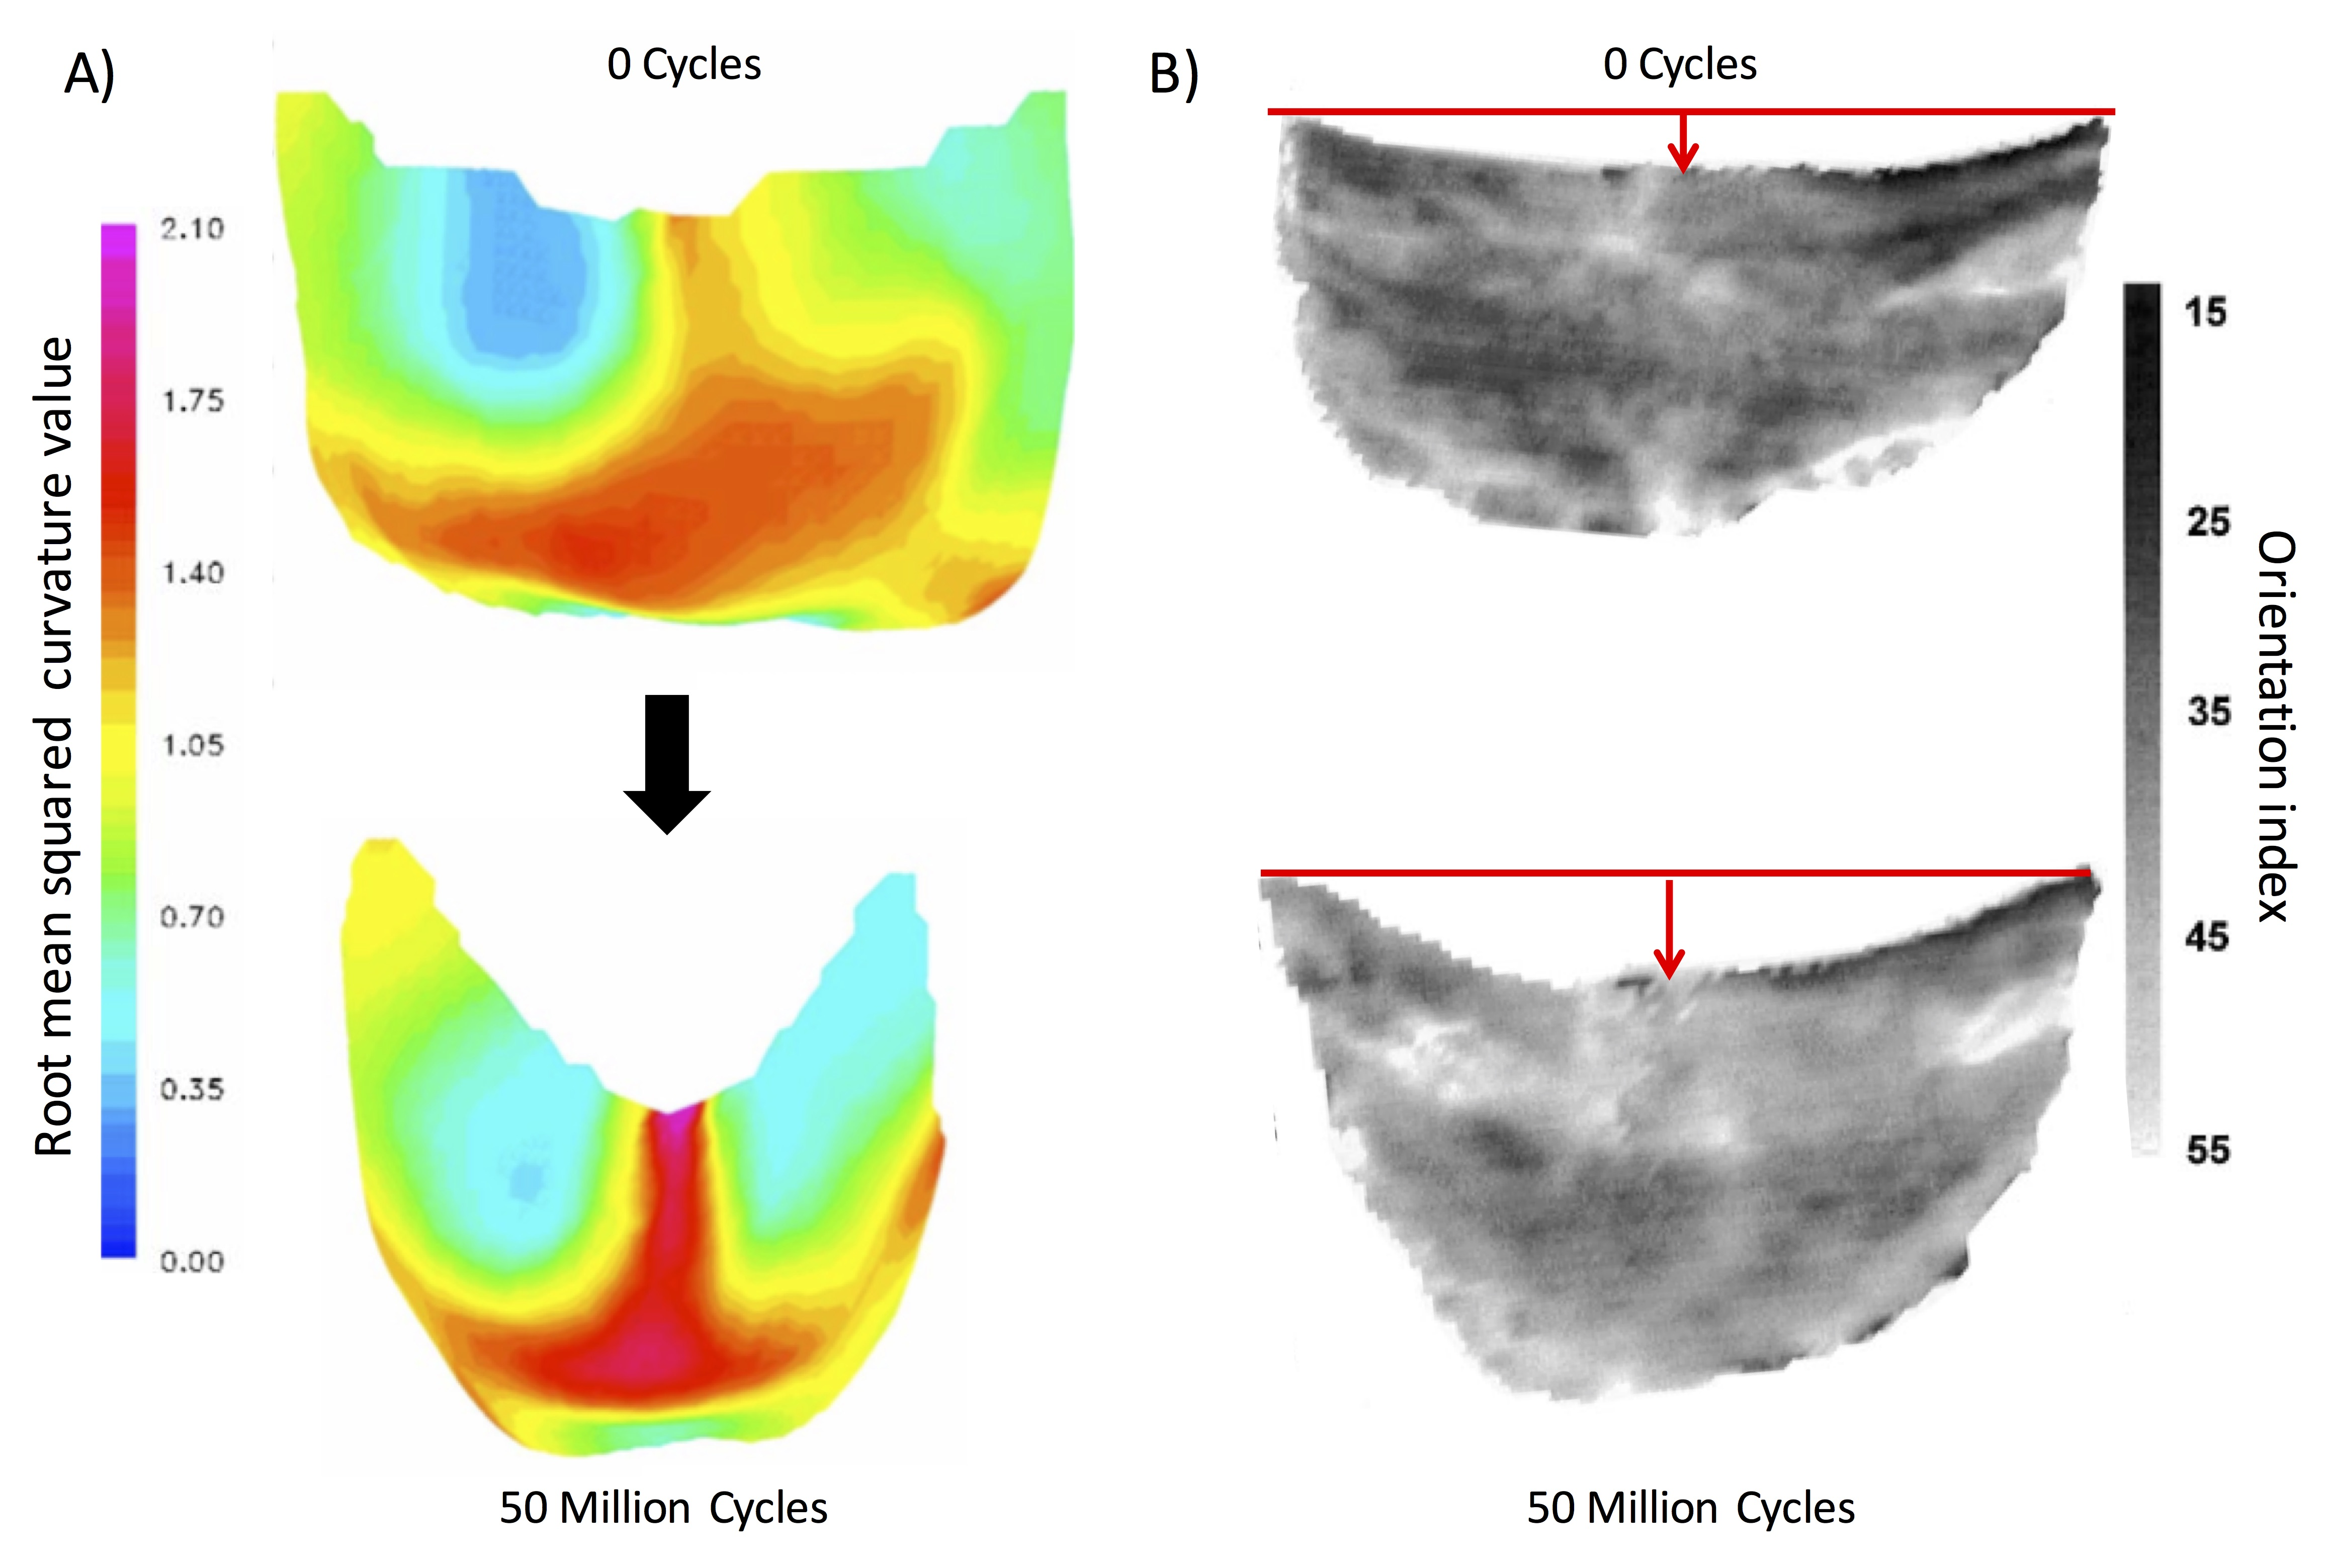
\includegraphics[width=\textwidth]{Images/chapter4/figure1}
\caption{A) The 3D unloaded geometry a BHV leaflet before and after cyclic loading, with the color indicating the local root mean squared curvature. The most significant change in geometry is in the belly region. B) BHV leaflet collagen fiber architecture, showing that the collagen fiber architecture are convected by the dimensional changes. The grayscale scale bar shows the orientation index (OI), which is angle containing 50 \% of fibers. The lack of changes in the OI suggests that minimal damage to the collagen fiber architecture has occurred.}
\label{fig:PSeffects}
\end{figure}


%%%%%%%%%%%%%%%%%%%%%%%%%%%%%%%%%%%%%%%%%%%%%%%%%%%%%%%%%%%%%%%%%%%%%%%%%%%%%%%%
%%%%    Exogenous crosslinking

\subsection{The effect of exogenous crosslinking}

	Bovine pericardium (BP) is a dense collagenous tissue composed mostly of collagen type I fibers with some elastin, GAGs, cells and vasculature. Collagen fibers are complex protein structures at the 2 - 10 $\mu$m scale, composed of tightly bundled collagen fibrils, which are approximately 50 nm in diameter. Much of what we know about the use of GLUT to exogenously crosslink collagenous tissue is from Nimni \textit{et al.} \cite{cheung_mechanism_1990, nimni_chemically_1987, cheung_mechanism_1985, gendler_toxic_1984, cheung_presence_1983, cheung_mechanism_1982, cheung_mechanism_1982II}. GLUT, which is an aldehyde based crosslinker, aggressively crosslinks free amines in proteins. This suppresses immunogenicity by crosslinking all cell membrane protein remnants, but also forms polymeric networks (at the nm scale) which allow for long range crosslinks to the nearby tissue microstructures. We previously found that exogenous crosslinking increases the bending stiffness of the matrix by four time the original stiffness \cite{mirnajafi_effects_2010}. We also tested the mechanical response of exogenously crosslinked BP before and after crosslinking, and developed the first constitutive model for exogenously crosslinked soft tissue \cite{sacks_novel_2016}. Interestingly, we also found that exogenously crosslinking does not increase the collagen fiber modulus, but significantly increases the interactions between collagen fibers \cite{sacks_novel_2016}, which is responsible for up to 30\% of the stress in the fully loaded state. 


	The GLUT crosslinking process involves a Schiff-base reaction. Importantly, the molecular bonds formed from Schiff-base reactions are known to be unstable at room and temperatures \cite{migneault_glutaraldehyde_2004, damink_glutaraldehyde_1995}. Thus, although GLUT is highly reactive and aggressively crosslinks extracellular matrix proteins, any resulting crosslinks will also readily undergo hydrolysis at body temperature \cite{migneault_glutaraldehyde_2004}. As a result, under cyclic loading in-vivo, exogenous ECM crosslinks will constantly break and reform. This continual process will cause the reference configuration to evolve towards the current loaded state. \emph{We thus hypothesize that this scission-healing behavior could be linked to the mechanisms that underlie how the BHV leaflet geometry evolves over time}.
	
	
    This damageless change in the BHV geometry has many similarities to the permanent set (PS) mechanisms observed in elastomers. Permanent set is an irreversible deformation that remains after a structure or material has been subjected to external stresses and then released. It does not involve damage to the constituents of the material, but instead changes the referential configuration. Although the outcomes may be similar, \emph{this form of permanent set is not a plastic deformations}, as they are entirely within the elastic regime. In particular, it has been used to model the scission-healing reactions of elastomers that occur when stretched, heated, cooled, then unloaded. This results in some of the materials to change in referential configuration to the loaded state. In this process, permanent set does not damage the polymeric fibers but is a result of the change in configuration of the underlying polymeric fiber network. Some works on constitutive models of this process include the works of Rajagopal and Wineman \cite{rajagopal_constitutive_1992}, Andrews and Tobolsky \cite{andrews_theory_1946}, and Rottach \textit{et al}. \cite{rottach_effect_2004, rottach_molecular_2007, rottach_permanent_2006}. However, there are little known studies on the permanent set effect in soft tissues or soft tissue derived exogenously crosslinked biomaterials. 
	

	\emph{Based on the above considerations, we hypothesize that the initial time evolving BHV geometry and mechanical response can be predicted by permanent set mechanisms}. Rather than heating and cooling, we assume that permanent set in exogenously crosslinked tissue occurs continuously at body temperature due to the GLUT, allowing the reference configuration of the exogenously crosslinked matrix (EXL matrix) to evolve over time. As a result, the reference configuration of BHVs will change while not affecting the intrinsic material properties of their constituents such as collagen fibers and the EXL matrix. Since the BHVs deform into a new configuration (Fig. \ref{fig:PSeffects}), there may develop regions of stress concentrations. The high stresses will increase the rate of structural damage and thus accelerate the rate of BHV failure. Thus, \emph{by compensating for the permanent set effects, it may be possible to reduce the BHV leaflet stresses and thus reduce structural damage to BHVs during \textit{in vivo} operation after implant.} Therefore, constitutive models that can predict the effects of permanent set are crucial for the simulation of BHVs. 

		
%%%%%%%%%%%%%%%%%%%%%%%%%%%%%%%%%%%%%%%%%%%%%%%%%%%%%%%%%%%%%%%%%%%%%%%%%%%%%%%%
%%%%    Constitutive models

\subsection{Constitutive models for the permanent set effect for soft tissues}

	The only work in the simulation of the permanent set effect in native or exogenously crosslinked soft tissues is the pioneering study of Martin and Sun \cite{martin_modeling_2013}, who developed a time dependent constitutive model for uniaxial cyclic loading of GLUT exogenously crosslinked BP strips using a damage analog. Briefly, to model the uncycled mechanical response, they used the Fung hyperelastic model for the strain energy density function, $\Psi_0$. The time dependent stress softening was then described using a modification to the strain energy function as $\Psi_\mathrm{PS} = (1-D_s)\Psi_0 - \Psi_0(\mathbf{E}_\mathrm{PS})$. Here the strain energy of the material after permanent set ($\Psi_\mathrm{PS}$) is reduced from $\Psi_0$ in accordance with a scaled damage function $D_s$ and the same strain energy function evaluated at the current amount of permanent set ($\mathbf{E}_\mathrm{PS}$). Martin and Sun then measured the maximum permanent set deformation that occurs for each specimen, and used that to set the maximum bound of $\mathbf{E}_\mathrm{PS}$. Additionally, Martin and Sun set two parameters, a lowerbound below which no permanent set occurs, and an upperbound above which the tissue fails. In the intermediate region, $D_s$ and $\mathbf{E}_\mathrm{PS}$ simply increase linearly with the number of cycles. The number of cycles needed to reach the maximum permanent set deformation was then described using an inverse exponential like function of the maximum strain applied, which is an analogous to the stress versus cycles (S–N) curve used to describe the fatigue behavior of traditional engineering materials. However, such approaches have the following limitations: 1) they are not predictive as there are no underlying mechanisms in the model. A damage-like model can mimic the results of permanent set but cannot explain nor predict the mechanisms responsible in exogenously crosslinked tissue, and 2) there is no way to extrapolate for predicting into unmeasured regimes using the Fung hyperelastic model. Therefore, there is a need for a more predictive constitutive model that utilizes the underlying mechanisms.


%%%%%%%%%%%%%%%%%%%%%%%%%%%%%%%%%%%%%%%%%%%%%%%%%%%%%%%%%%%%%%%%%%%%%%%%%%%%%%%%
%%%%    A new approach

\subsection{A new approach for modeling the permanent set effect in exogenously crosslinked soft tissues}

	We utilize a structural constitutive modeling approach, which integrates information on tissue composition and structure for material characterization \cite{sacks_structural_2000}. In principal, using structural models we only need to perform parameter estimation for the intrinsic material properties, such as collagen fiber modulus and EXL matrix modulus, to predict the mechanical response using the quantified tissue microstructure. This mechanism based approach allows us to predict the mechanical response at strains outside of the strain range of the experimental data used for parameter estimation \cite{zhang_meso_2016, fata_insights_2014}; a feat not possible using purely phenomenological approaches. In addition, by using a structural modeling approach coupled with the permanent set mechanism to predict the collagen fiber architecture after cyclic loading, we can also predict the mechanical response of the soft tissue at higher cycle numbers. Thus, we use 1) the structural model parameters obtained in the uncycled mechanical state and 2) the permanent set mechanisms to predict how the mechanical response of the exogenously crosslinked tissues evolves with cyclic loading. The key aspects of our approach include:
\begin{enumerate}
\item Model the change in mechanical response entirely as a kinematic change in the underlying microstructure; no actual change in mechanical properties (damage)
\item Predict the change in geometry from the loading history and the permanent set mechanism
\item Validate the permanent set mechanism under both strain and stress controlled loading conditions
\item Develop a time dependent implementation with an evolving loaded configuration under stress control
\end{enumerate}

%---    Experimental methods and data post-processing
%%%%%%%%%%%%%%%%%%%%%%%%%%%%%%%%%%%%%%%%%%%%%%%%%%%%%%%%%%%%%%%%%%%%%%%%%%%%%%%%
%% Overall Approach
%%%%%%%%%%%%%%%%%%%%%%%%%%%%%%%%%%%%%%%%%%%%%%%%%%%%%%%%%%%%%%%%%%%%%%%%%%%%%%%%


\section{Overall modeling approach} \label{sec:modelapproach}

	We hypothesize that permanent set and structural damage are two separate and largely sequential mechanisms that underlie the mechanical response of BHVs. Thus, the life span of BHVs can by separated into three stages: early (up to 2-5 years),  intermediate (up to 10 years), and late stage (up to failure) (Fig. \ref{fig:hypothesis}). In the early stage, permanent set induces significant changes in BHV geometry while structural damage does not play a detectable role. This leads to increased stress and structural damage in the intermediate term which leads to failure in the late term. Thus, by compensating for the effect of permanent set on the geometry, we hypothesize that we can extend the life span of BHVs. We focus our model on the early stage of cyclic loading and build a solid foundation for modeling and simulating the later stages.


\begin{figure}[hbt]
\centering
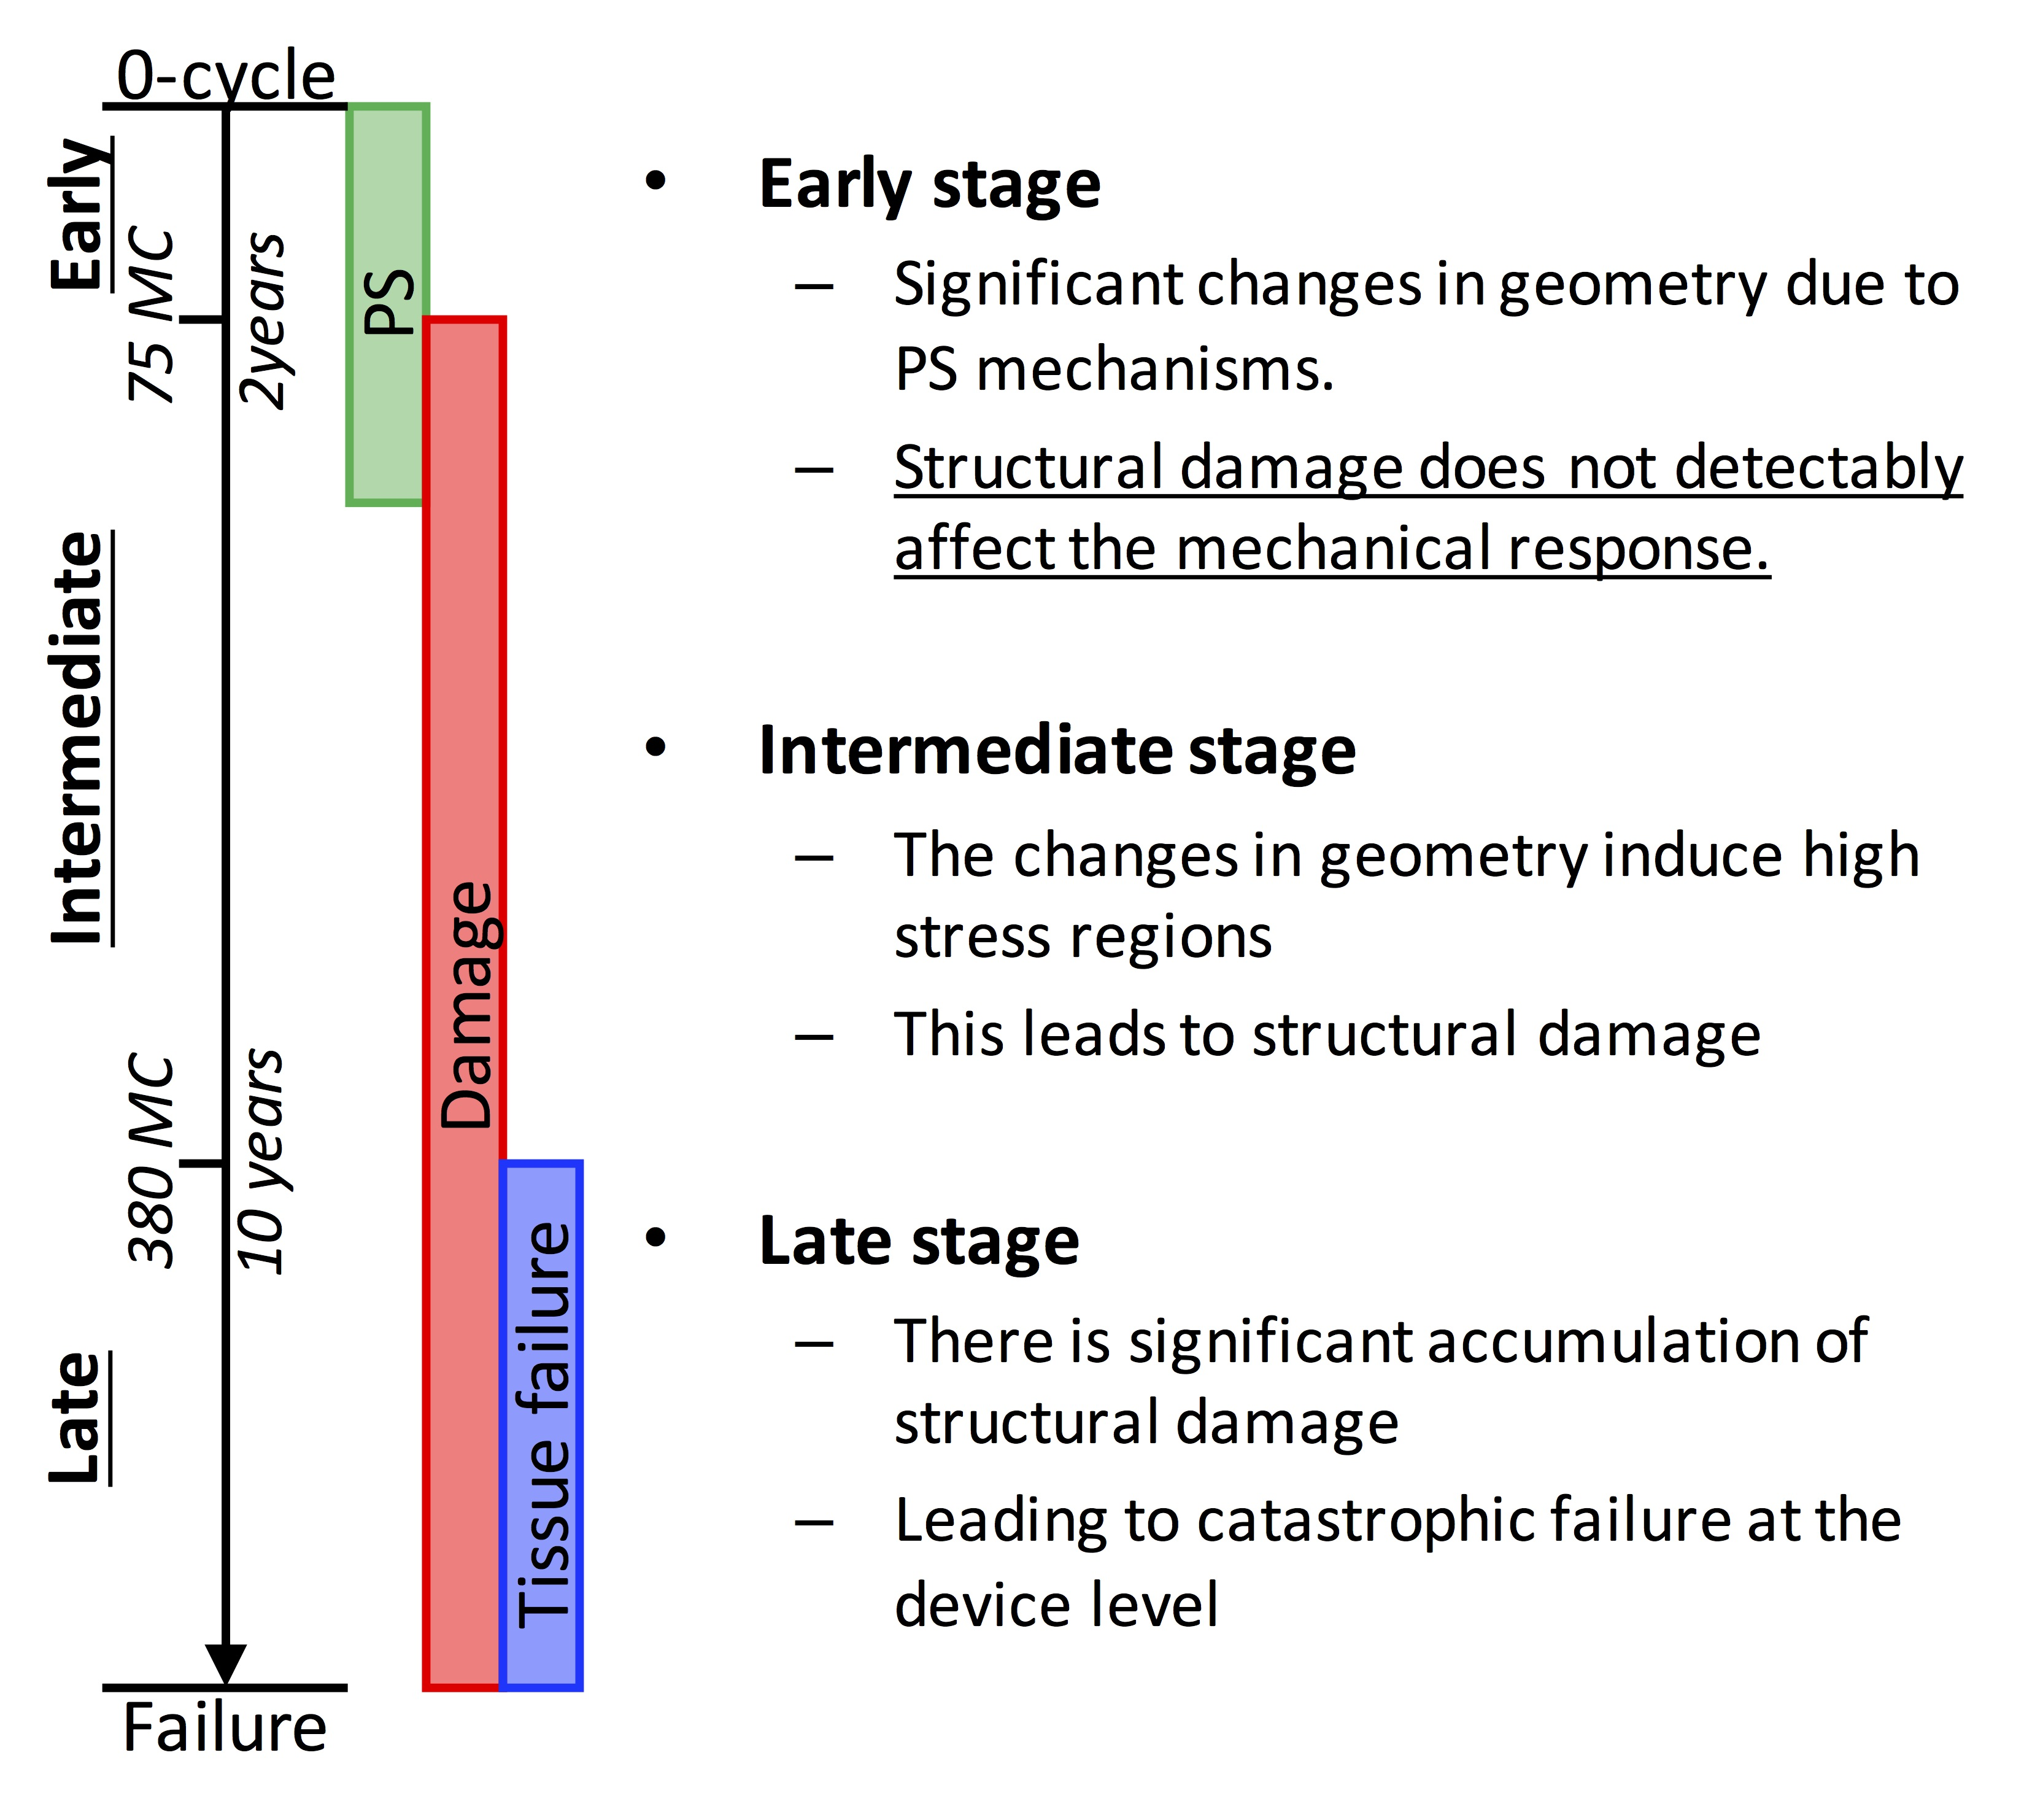
\includegraphics[width=4in]{Images/chapter4/figure2}
\caption{We speculate that the progression of structural damage and permanent set of BHV leaflets progress during long term cyclic loading can be separated into three stages: early, intermediate, and late.}
\label{fig:hypothesis}
\end{figure}


	We assume that permanent set is driven by the scission-healing behaviors of the GLUT polymer network in the non-fibrous EXL matrix, allowing for fractions of it to change in reference state (Fig. \ref{fig:PS}A). The formation of aldehyde bonds during crosslinking, as well as the occasional hydrolysis of the aldehyde bonds follows \emph{first order molecular kinetics} \cite{migneault_glutaraldehyde_2004}. Since this process drives the scission-healing of GLUT polymers and thus permanent set, we hypothesize that permanent set also follows first order kinetics. In addition, we note that the length scale of crosslinks formed by GLUT polymers ($\mathrm{nm}$) in the EXL matrix is several orders of magnitude smaller than that of the collagen fibers ($\mu \mathrm{m}$). Thus, we assume that the collagen fiber architecture does \emph{not} undergo scission-healing like the EXL matrix. Instead, the collagen fibers remain intact during cyclic loading. Rather, the collagen fiber architecture is convected by the changes in geometry that occurs with permanent set in the EXL matrix (Fig. \ref{fig:PS}B). \emph{We refer to this mechanism as structural convection, which is defined as applying a permanent deformation (elongation and rotation of collagen fibers, Fig. \ref{fig:structuralconvection}) to the collagen fiber architecture based on the change in the reference configuration}. Previously, we have shown that dense collagenous tissues deform under affine kinematics \cite{lee_presence_2015}. Since deformations during cyclic loading are in the elastic regime and cyclic loading (second) is on a time scale much shorter than that of permanent set (weeks), the only change in collagen fiber architecture on a cycle to cycle period is also under affine kinematics. Therefore, we also assume that the convection of collagen fiber architecture due to permanent set is under affine kinematics as well. Thus, our approach is based on using the permanent set effect to model the evolving properties of the EXL matrix, determine the change in reference configuration and convect collagen fiber architecture, which then allows us to determine the change in mechanical response of the collagen fibers using structural models. 


\begin{figure}[hbt]
\centering
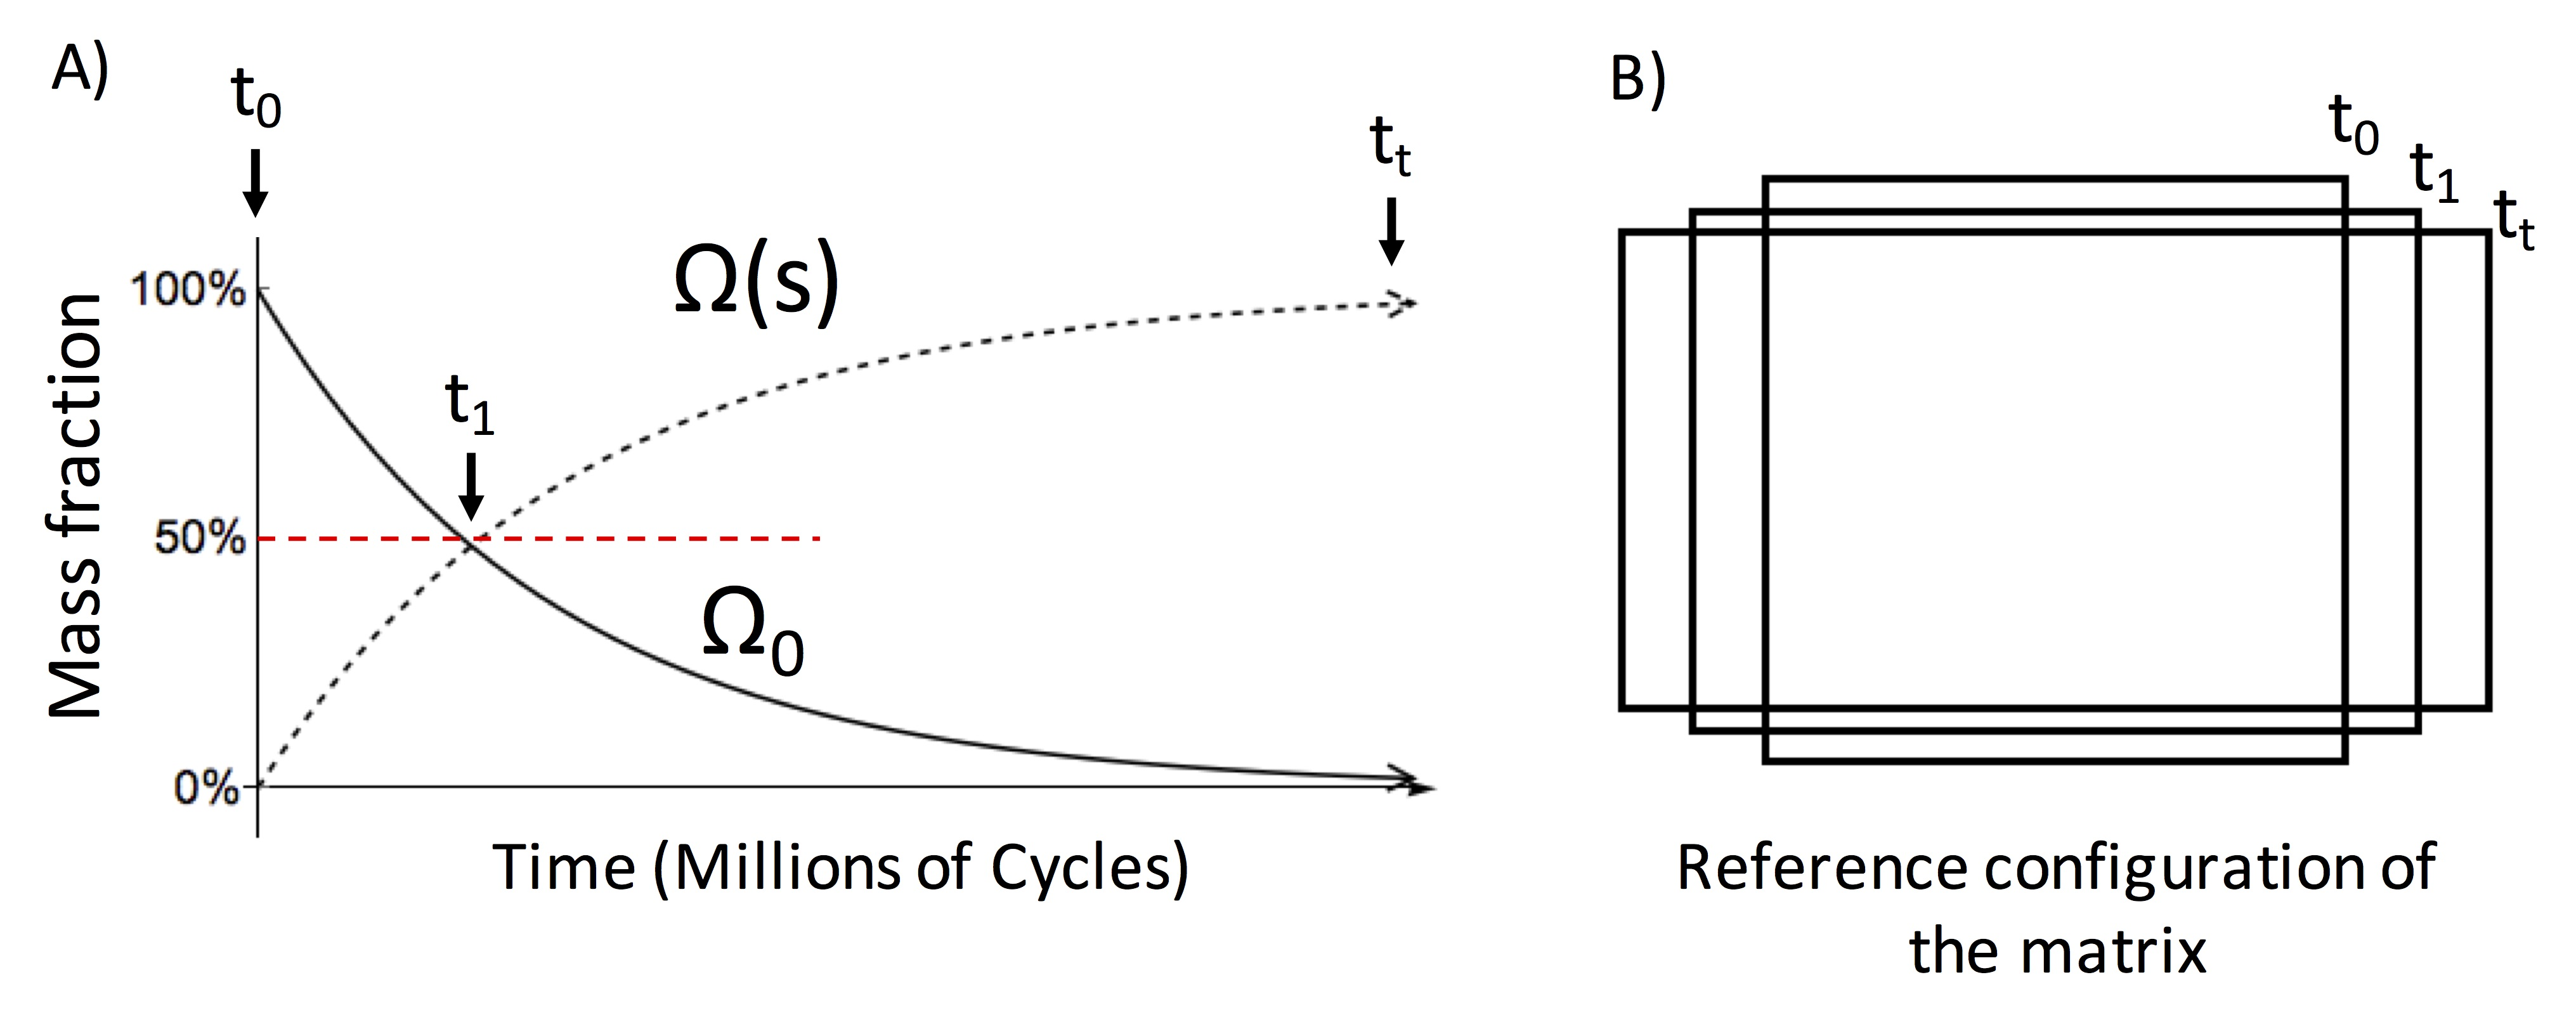
\includegraphics[width=\textwidth]{Images/chapter4/figure3}
\caption{Illustration of the permanent set effect under cyclic uniaxial loading. A) There is a transfer of mass fraction of the EXL matrix to the loaded configuration $\Omega(s)$ from the original state $\Omega_0$. B) This results in changes in the unloaded geometry of the tissue.}
\label{fig:PS}
\end{figure}

\begin{figure}[hbt]
\centering
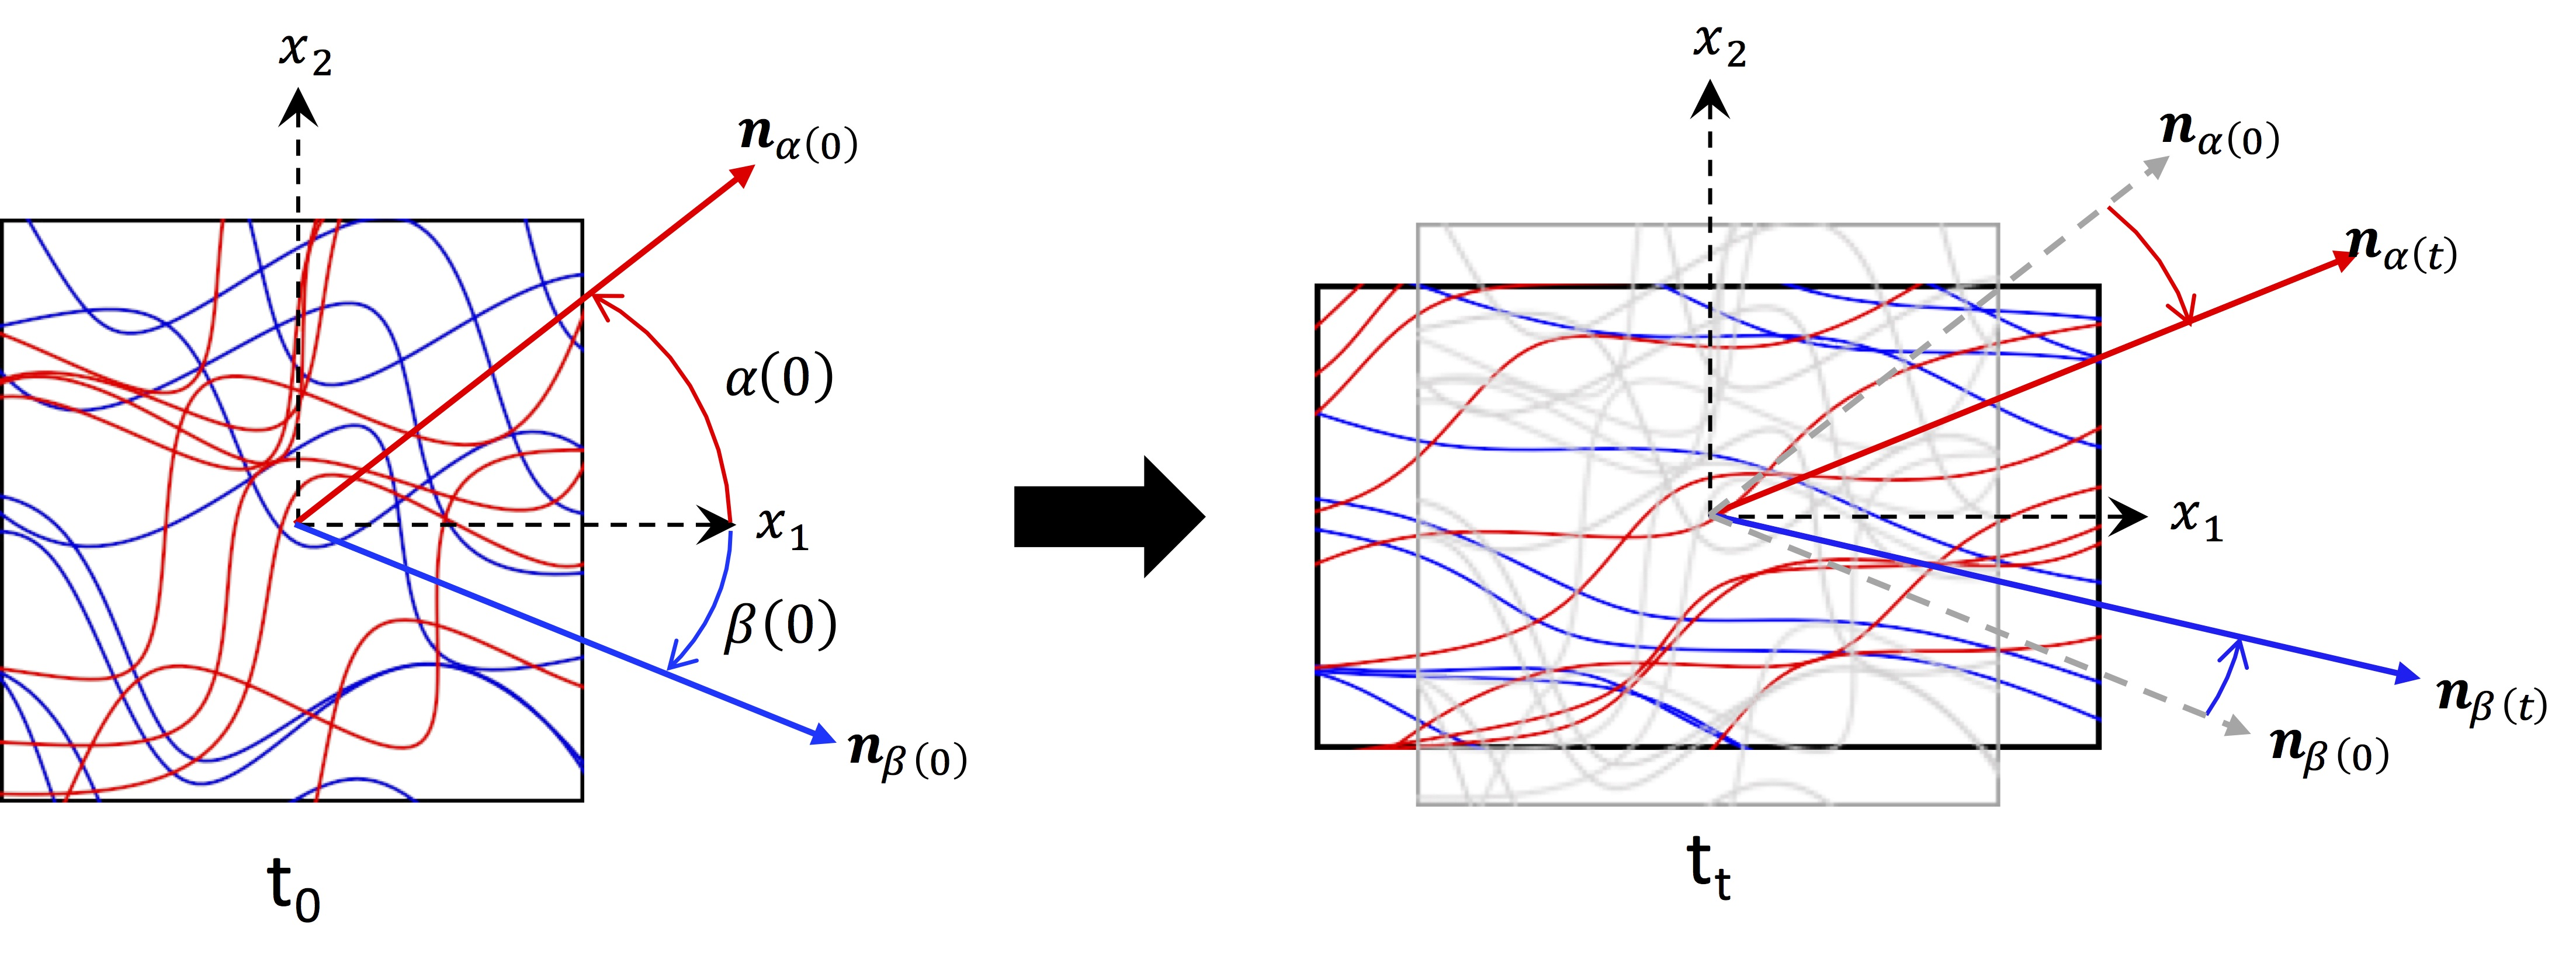
\includegraphics[width=\textwidth]{Images/chapter4/figure4}
\caption{An illustration of how the collagen fiber architecture is convected by changes in the dimension of the bulk tissue. The left figure shows the origin geometry of the tissue at $\mathrm{t}_0$ in figure \ref{fig:PS} while the right figure shows the geometry of the tissue at $\mathrm{t}_t$. Structural convection includes the rotation and straightening of the collagen fiber ensembles. }
\label{fig:structuralconvection}
\end{figure}


	To develop the constitutive model form, we start by modeling the exogenously crosslinked tissue under cyclic loading as parts of a mixture of materials with the same properties but different evolving reference states. The reference state of each part of the EXL matrix is updated according the strain history (Fig. \ref{fig:PS}A). The response of each part are then summed together for the bulk-level mechanical response of the EXL matrix. The new bulk level mechanical response is then used to determine the new unloaded state (Fig. \ref{fig:PS}B). The change in the EXL matrix from its uncycled state is then used to convect the collagen fiber architecture(Fig. \ref{fig:structuralconvection}). The new mechanical response of the EXL matrix is summed with the fiber ensemble interactions and collagen fiber response predicted from the new collagen fiber architecture to determine the full tissue-level mechanical response. Thus, how the \emph{collagen fiber architecture (CFA) is convected by the EXL matrix} is crucial to our model. We start developing our constitutive model by 1) modeling and parameter estimation for the native uncycled mechanical response of the exogenously crosslinked tissue. Then 2) develop the model form for the time evolving mechanical response based on the permanent set mechanism and cyclic loading data. The basic assumptions of our models are:
\begin{enumerate}
\item There is no structural damage to the collagen fibers or the EXL matrix
\item The crosslinking process that induce permanent set follows first order kinetics
\item We are only modeling permanent set under physiological conditions and the process is thus isothermal
\item Permanent set occurs in the isotropic EXL matrix, so that its rate constant is directionally independent
\item The permanent set rate constant is strain-level independent in the physiological range
\item Permanent set occurs over a time scale much longer than a single cardiac cycle
\item The tissue is functionally elastic, and thus viscoelastic effects are ignored
\item The convection of the collagen fiber architecture follows affine kinematics
\item collagen fibers do not bare load or interact until they are straightened
\cite{lee_presence_2015}
\end{enumerate}



%---    Delineation and modelling of the tissue-level mechanical effects of exogenous cross-links
%%%%%%%%%%%%%%%%%%%%%%%%%%%%%%%%%%%%%%%%%%%%%%%%%%%%%%%%%%%%%%%%%%%%%%%%%%%%%%%%
%%  Experimental Data
%%%%%%%%%%%%%%%%%%%%%%%%%%%%%%%%%%%%%%%%%%%%%%%%%%%%%%%%%%%%%%%%%%%%%%%%%%%%%%%%


\section{Extant experimental data}
\label{sec:database}

	We utilized data from the following two extant studies, which differ by their loading conditions and specimen orientations. In the study by Sun \textit{et al}.\cite{sun_response_2004}, exogenously crosslinked BP patches were cycled along the preferred collagen fiber direction (PD) at a peak strain of 16\% and maintained for up to 65 million cycles (Fig. \ref{fig:database}A\&B). The reference configurations of the exogenously crosslinked BP were tracked using fiducial markers attached to the center of the specimens\cite{sacks_biaxial_2000}. The mechanical cycling was stopped at 30 and 65 million cycles for mechanical testing with multiple protocols and different loading paths. It was found that there were significant extensions in the direction of loading (7.1\%), PD, and contractions in the cross direction (-7.7\%). In addition, the collagen fiber crimp period increased from 40.6$\mu$m to 45.24$\mu$m which is consistent with the convection of the collagen fiber architecture that would occur as collagen fiber straighten (Fig. \ref{fig:structuralconvection}). The mechanical response also changed accordingly. The compliance in the PD decreased over time while the compliance in the cross direction of the tissue increased. 
	

\begin{figure}[hbt]
\centering
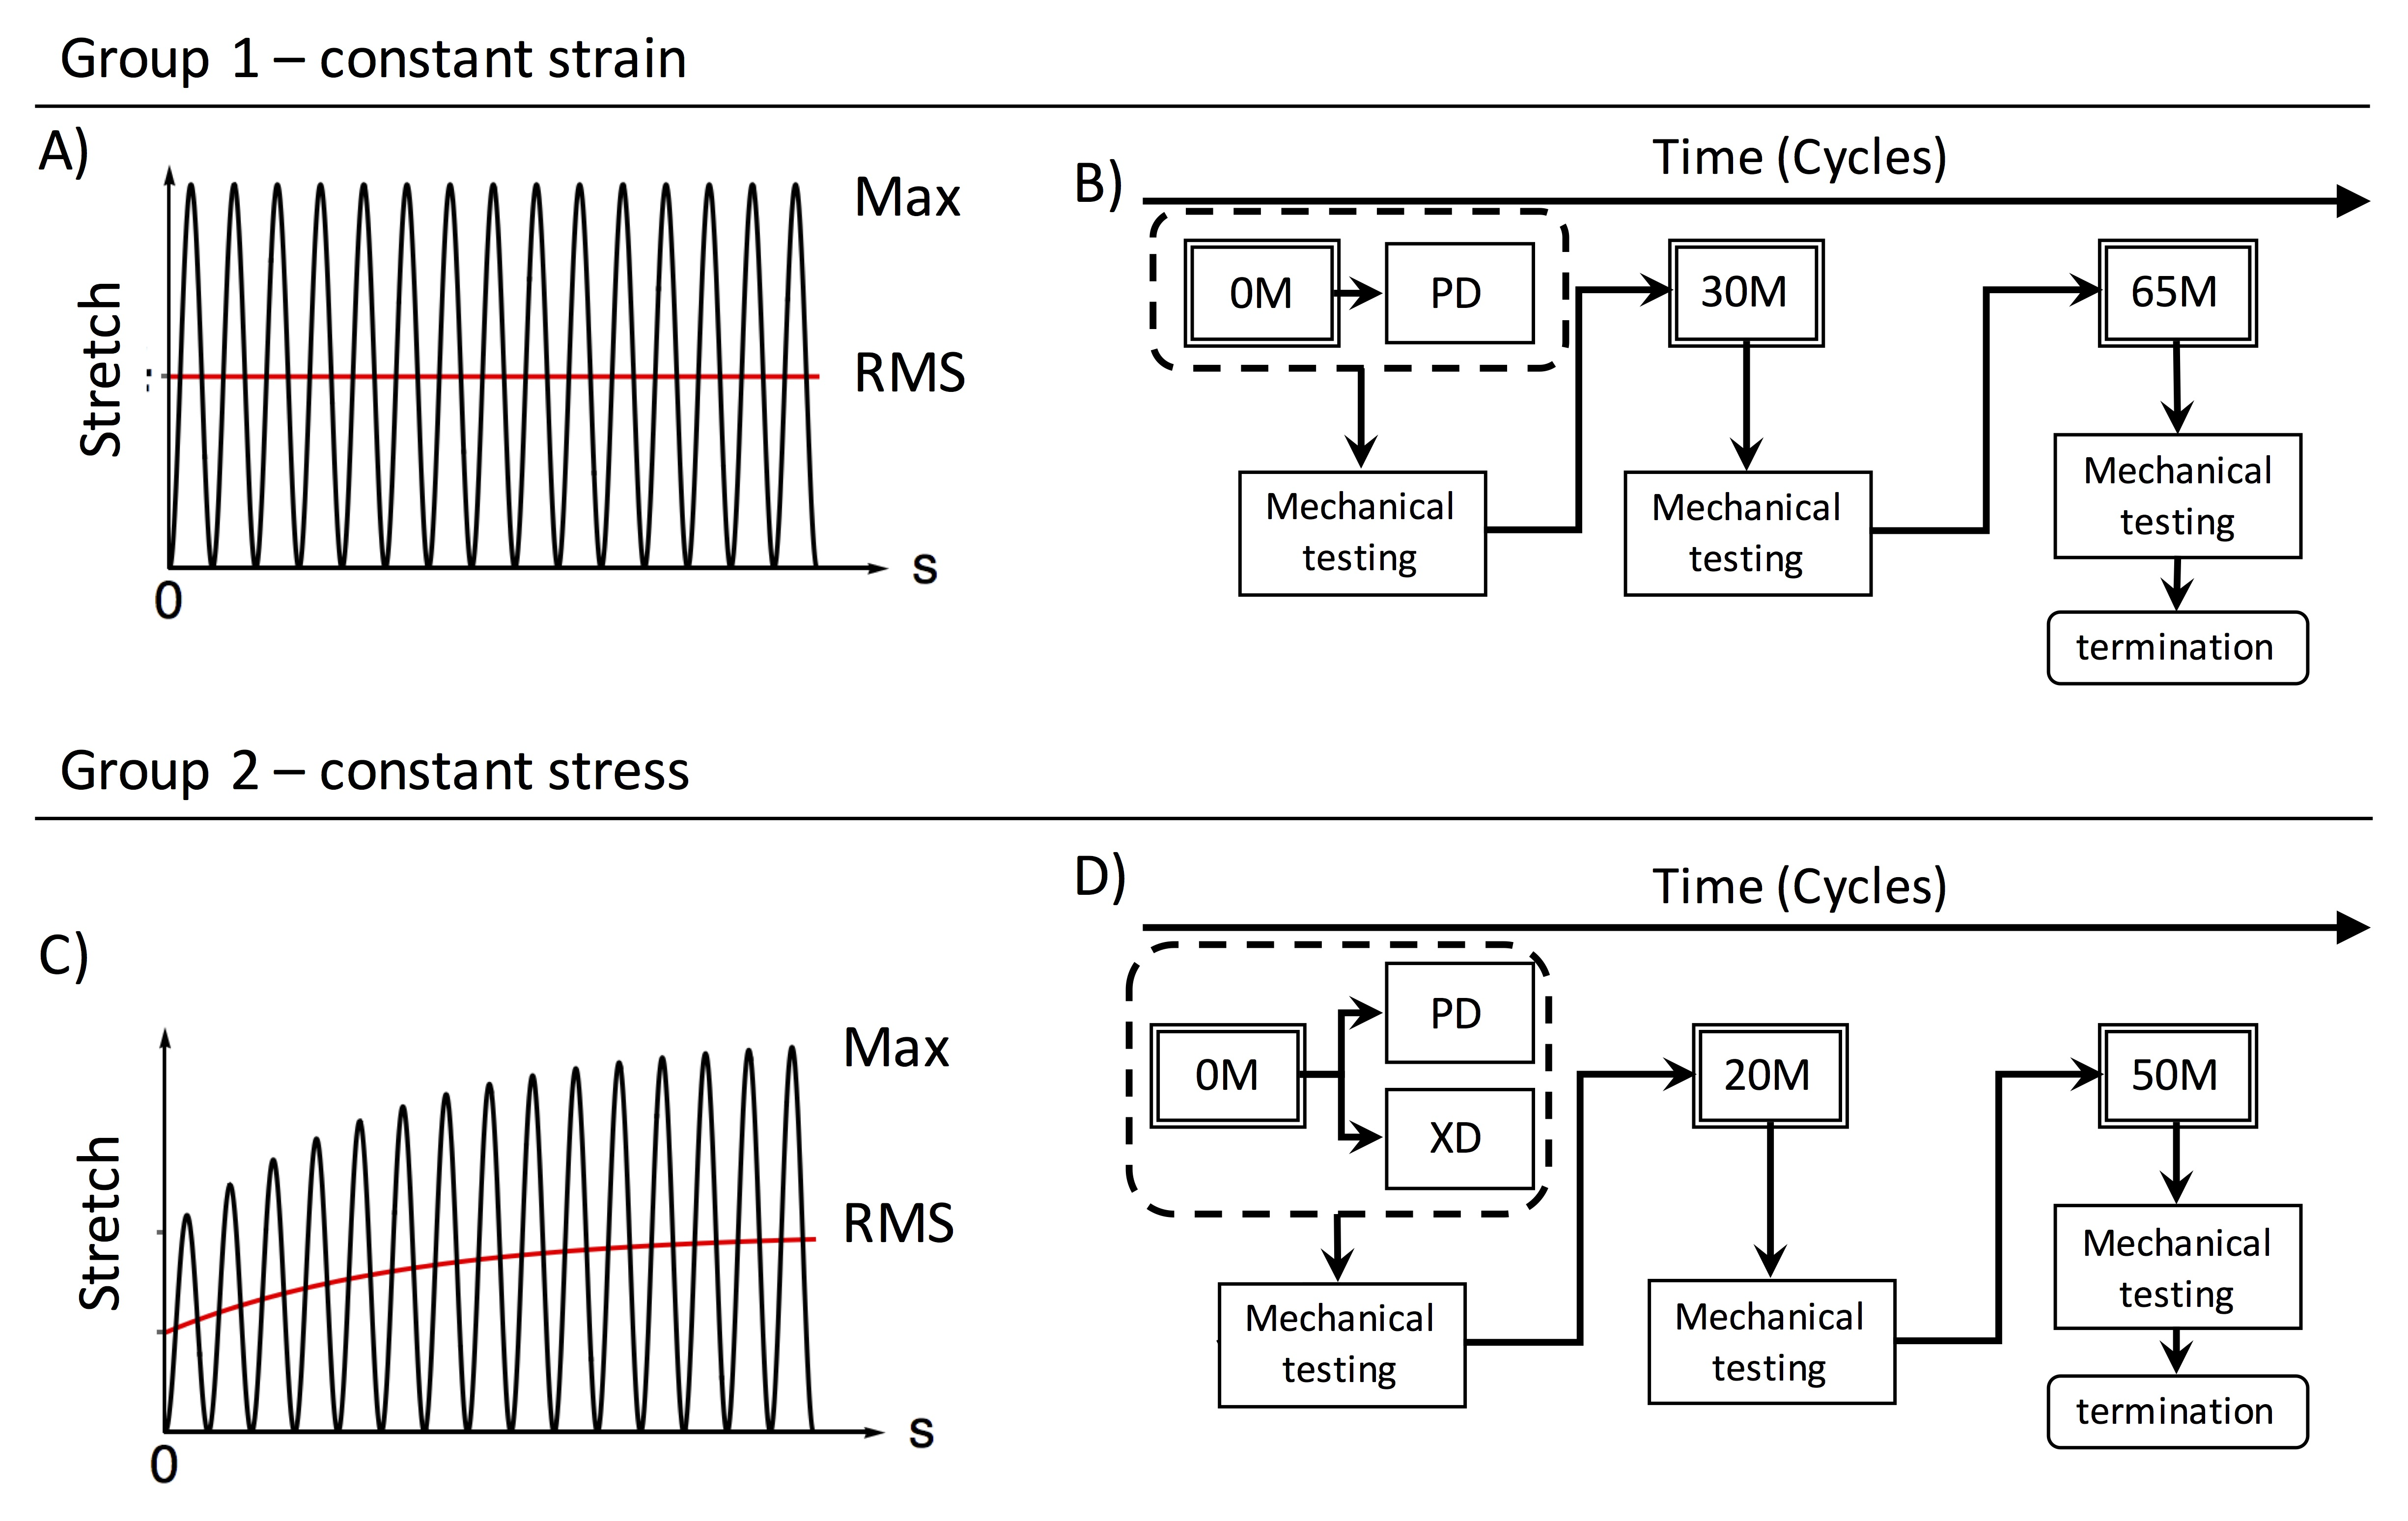
\includegraphics[width=\textwidth]{Images/chapter4/figure5}
\caption{We utilize two extant databases in this study. The first is strain controlled, with A) constant strain level and is B) sorted for orientation along the preferred direction then put through cyclic loading and mechanical testing. The second is with C) constant strain but evolving strain level. The specimens are then D) sorted for orientation along both the preferred direction and cross-preferred direction, then put through cyclic loading and mechanical testing.}
\label{fig:database}
\end{figure}



	In the study by Sellaro \textit{et al}.\cite{sellaro_effects_2007}, the same exogenously crosslinked BP patches were cycled at 500kPa for up to 50 million cycles (Fig. \ref{fig:database}C\&D). In this case, the specimens were separated into two groups: with stress controlled loading along the 1) PD and 2) orthogonal to the PD (XD). Similarly, the reference states of the exogenously crosslinked BP specimens were tracked, with cycling stopped at 20 and 50 million cycles for mechanical testing. Analysis of the results showed interesting differences between the PD and XD cycled specimens. For both the PD and XD cycled specimens, we observed significant elongation in the direction of loading and contraction in the orthogonal direction with cycling. Additionally, the effective stiffness in the direction of loading increased over time, whereas the orthogonal direction decreased over time. In addition, we also studied how the collagen fiber architecture of the tissue changed with cyclic loading. For the PD cycled specimens, it was observed that the collagen fiber orientation distribution became more aligned, and the collagen fiber crimp period increased from 24 $\mu$m to 28$\mu$m. On the other hand, for the XD cycled specimens, it was observed that the collagen fiber orientation distribution became more spread, and the collagen fiber crimp period remained unchanged. This findings on the structural changes with direction of cyclic loading are consistent with the structural convection that we hypothesizes with permanent set and lend further support to our model (Fig. \ref{fig:structuralconvection}). 

%---    Initial model formulation
%%%%%%%%%%%%%%%%%%%%%%%%%%%%%%%%%%%%%%%%%%%%%%%%%%%%%%%%%%%%%%%%%%%%%%%%%%%%%%%%
%%  Constitutive Model
%%%%%%%%%%%%%%%%%%%%%%%%%%%%%%%%%%%%%%%%%%%%%%%%%%%%%%%%%%%%%%%%%%%%%%%%%%%%%%%%


\section{Constitutive model for uncycled exogenously crosslinked tissue}

%%%%%%%%%%%%%%%%%%%%%%%%%%%%%%%%%%%%%%%%%%%%%%%%%%%%%%%%%%%%%%%%%%%%%%%%%%%%%%%%
%%%%    Constitutive Model for crosslinking

\subsection{Constitutive model for exogenous crosslinking}

	We have previously developed the first constitutive model for exogenously crosslinked collagenous tissues \cite{sacks_novel_2016} and determined the following three contributors to the mechanical response: collagen fibers, EXL matrix and fiber-fiber interactions, where the total strain energy density function is given by
\begin{equation} \label{eq:totalstrainenergy}
    \Psi = \phi_\mathrm{col} \left[ \Psi_\mathrm{col} + \Psi_\mathrm{int}\right] + \phi_m \Psi_m
\end{equation}
	In particular, we found the fiber ensemble interaction term ($\phi_\mathrm{col} \Psi_\mathrm{int}$) to be especially important in modeling exogenously crosslinked tissues, accounting for approximately 30\% of the stress in the fully loaded state (Fig. \ref{fig:EXLforms}A). To determine the model form of the interaction component, we used the remaining stress after subtracting the collagen fiber response and EXL matrix response from the mechanical response of the tissue after exogenous crosslinking (Fig. \ref{fig:EXLforms}A). In that study, we consider three possible forms of interactions: intra-fiber ensemble (Fig. \ref{fig:EXLforms}B) (an ensemble being a family of fibers sharing a common orientation), ensemble-ensemble rotations, and ensemble-ensemble relative extensions (Fig. \ref{fig:EXLforms}C\&D). We found that intra-fiber ensemble and ensemble-ensemble rotations were not consistent with the experimental data, whereas ensemble-ensemble extensional interactions were able to explain all of the remaining stress. 
	
\begin{figure}[hbt]
\centering
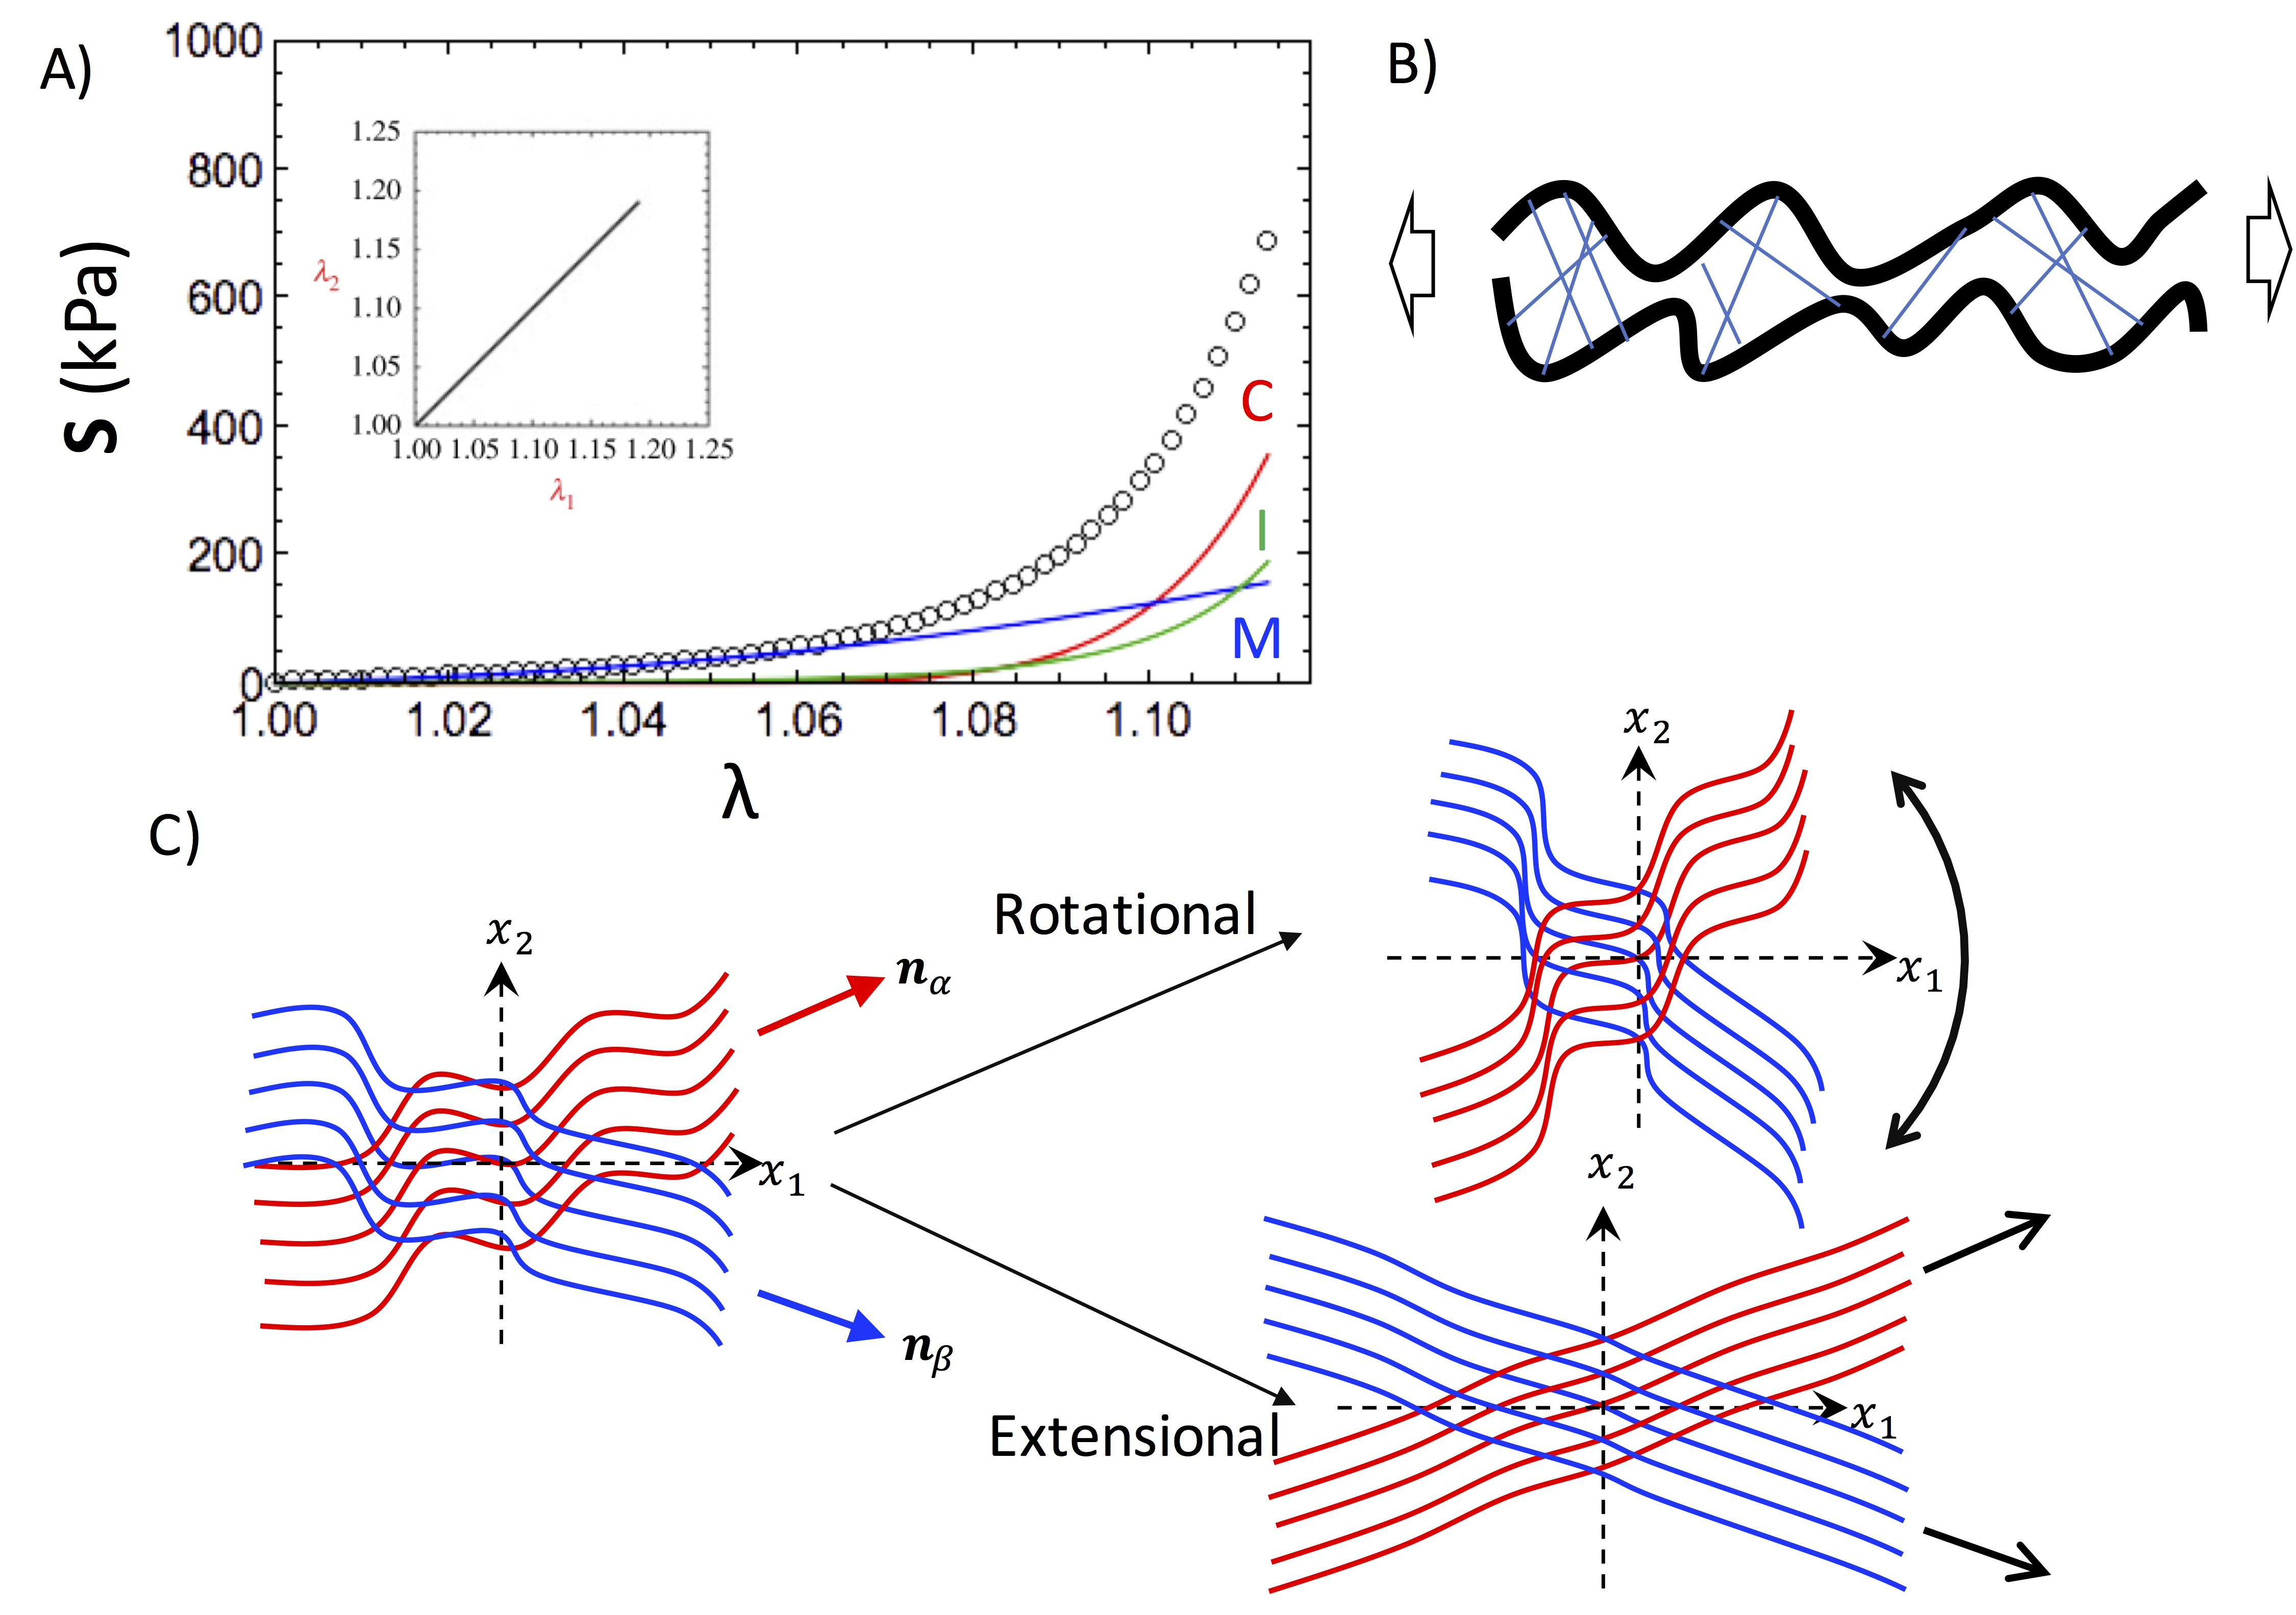
\includegraphics[width=\textwidth]{Images/chapter4/figure6}
\caption{A) The mechanical response of exogenously crosslinked BP, which is composed of 3 parts: (C)ollagen in Red, (M)atrix in Blue, and the fiber ensemble (I)nteractions in Green. B) Illustration for intra-ensemble interactions due to crosslinking is shown. C) The inter-ensemble interactions could be separated into rotational effects and extensional effects. }
\label{fig:EXLforms}
\end{figure}
	
    The interaction model form, $\Psi_\mathrm{int}$, was developed utilizing the pseudo invariant $I_8$, which is a function of the stretch and angle between two fiber ensembles oriented along the angle $\alpha$ and $\beta$ directions in the tissue (Fig. \ref{fig:structuralconvection}), and then separated it into its rotational and extensional components\cite{sacks_novel_2016} (Fig. \ref{fig:EXLforms}C\&D),
\begin{equation} \label{eq:I8invariant}
\begin{gathered}
I_8 = \mathbf{n}_ \alpha \cdot\mathbf{C}\cdot\mathbf{n}_\beta = \lambda_\alpha \lambda_\beta \cos(\alpha - \beta), \\
I_8^{\mathrm{ext}} = \lambda_\alpha \lambda_\beta, \qquad I_8^{\mathrm{rot}} = \cos(\alpha - \beta) = \frac{I_8}{\lambda_\alpha \lambda_\beta},
\end{gathered}
\end{equation}
    where $\mathbf{n}_\alpha$ and $\mathbf{n}_\beta$ are vectors pointing along $\alpha$ and $\beta$, respectively, $\lambda_\alpha$ and $\lambda_\beta$ are the stretches of the collagen fiber ensembles oriented along $\alpha$ and $\beta$, respectively , $I_8^\mathrm{ext}$ is the pseudo invariant for ensemble-ensemble extensions, and $I_8^\mathrm{rot}$ is the pseudo invariant for ensemble-ensemble rotations. From this, we established the model form for the interactions to be
\begin{equation}
\Psi_{\mathrm{int}} = \frac{d_0}{4}\int\displaylimits_\alpha \int\displaylimits_\beta \Gamma\left(\alpha\right)\Gamma \left( \beta \right)\left[ e^{d_1(\lambda_\alpha \lambda_\beta - 1)^2}-1 \right] \mathrm{d}\alpha\, \mathrm{d}\beta,
\end{equation}
    where $\Gamma$ is the fiber orientation distribution (ODF), and $d_0$ and $d_1$ are material constants. 
	However, this model form is still essentially phenomenological. 
	Specifically, while it is sufficient to model the mechanical response in the range of the acquired experimental data, we have no method for predicting how it will change with changes in dimensions with cyclic loading. Thus, an extension to this model component is necessary.

%%%%%%%%%%%%%%%%%%%%%%%%%%%%%%%%%%%%%%%%%%%%%%%%%%%%%%%%%%%%%%%%%%%%%%%%%%%%%%%%
%%%%    Extension for structural model

\subsection{Extension of the structural derivation of the fiber-fiber interactions term}

    The key to our approach in the constitutive model for the permanent set effect is to use the change in the collagen fiber architecture to predict the new mechanical response. Thus, having a full structural model, including a full structural derivation of the fiber-fiber interactions, is crucial. As in the previous model form \cite{sacks_novel_2016}, we will only keep the extensional component $I_8^\mathrm{ext}$. In addition, since collagen fibers do not bear stress until fully straightened \cite{soares_biomechanical_2016}, we also assume that \emph{collagen fibers do not play a role in the interactions of the fiber ensembles until they are straightened}. Following the same approach common in structural models, we first define the stretch of the collagen fibers after it's straightened, which is also the true fiber stretch ($\lambda_t$) defined in Zhang et al. \cite{zhang_meso_2016}, to be $\lambda_t = \lambda_\mathrm{ens}/\lambda_s$, where $\lambda_\mathrm{ens}$ is the stretch of the collagen fiber ensemble and $\lambda_s$ is the slack stretch required to straighten the collagen fiber crimp. We assumed that interactions do not occur until the fibers are straighten, so the extensional invariant should be a function of the true stretch of the individual fibers, $\lambda_t$, rather than the stretch of the whole fiber ensembles as defined in equation \ref{eq:I8invariant},
\begin{equation}
I_8^{\mathrm{ext}} = \frac{\lambda_\alpha \lambda_\beta}{\prescript{}{\alpha}{\lambda}_s \prescript{}{\alpha}{\lambda}_s},
\end{equation}
    where $\prescript{}{\alpha}{\lambda}_s$ and $\prescript{}{\beta}{\lambda}_s$ are the slack stretches of the two ensembles oriented along $\alpha$ and $\beta$ in the reference configuration, respectively. This invariant is then integrated only for fibers with $\lambda_t > 1$, i.e. fibers which are straightened. To develop the form for the interactions, we start from the strain energy. At the ensemble level, we integrate the invariant over the slack stretch $(\lambda_s)$ of both the fiber ensembles orienting along $\alpha$ and $\beta$, weighted by the probability distribution function of the proportion of collagen fibers with that specific slack stretch $D(\lambda_s)$,
\begin{equation}
\Psi_{\mathrm{int}}^{\mathrm{ens}} = \frac{\eta_I}{2} \int\displaylimits_1^{\lambda_\alpha} \int\displaylimits_1^{\lambda_\beta} D\left( x_\alpha \right) D\left( x_\beta \right) \left( \frac{\lambda_\alpha \lambda_\beta}{x_\alpha x_\beta} - 1\right)^2 \,\mathrm{d}x_\alpha \,\mathrm{d}x_\beta.
\end{equation}
    We refer to $D(\lambda_s)$ as the recruitment function, which is defined in Zhang et al. \cite{zhang_meso_2016}. The ensemble-level model is then integrated with respect to the fiber ODF, $\Gamma$, for all possible pair of collagen fiber ensemble to give the tissue-level model
\begin{equation}
\Psi_{\mathrm{int}} = \frac{\eta_I}{2} \int\displaylimits_\alpha \int\displaylimits_\beta \Gamma(\alpha) \Gamma(\beta) \int\displaylimits_1^{\lambda_\alpha} \int\displaylimits_1^{\lambda_\beta} D\left( x_\alpha \right) D\left( x_\beta \right) \left( \frac{\lambda_\alpha \lambda_\beta}{x_\alpha x_\beta} - 1\right)^2 \,\mathrm{d}x_\alpha \,\mathrm{d}x_\beta \,\mathrm{d}\alpha \,\mathrm{d}\beta.
\end{equation}
    The second Piola Kirchhoff stress, using $\mathbf{S}=2\frac{\partial\Psi}{\partial\mathbf{C}}$, is 
\begin{equation} \label{eq:interaction}
\begin{split}
\mathbf{S}_{\mathrm{int}} = \eta_I \int\displaylimits_\alpha \int\displaylimits_\beta \Gamma \left(\alpha \right) \Gamma \left( \beta \right) 
\left[ \left\lbrace 
\int\displaylimits_1^{\lambda_\alpha} \int\displaylimits_1^{\lambda_\beta} 
\frac{2 \lambda_\beta D(x_\alpha) D(x_\beta)}{x_\alpha x_\beta} 
\left( \frac{\lambda_\alpha}{x_\alpha} \frac{\lambda_\beta}{x_\beta} - 1\right) \mathrm{d}x_\alpha \, \mathrm{d}x_\beta \right.\right. +&\\
\left. \left. \int\displaylimits_1^{\lambda_\beta} D(x_\beta) \left( \frac{\lambda_\beta}{x_\beta} -1  \right)^2 \mathrm{d}x_\beta \right\rbrace \right.  \frac{\mathbf{n}_\alpha \otimes \mathbf{n}_\alpha}{\lambda_\alpha} +& \\
\left. \left\lbrace
\int\displaylimits_1^{\lambda_\alpha} \int\displaylimits_1^{\lambda_\alpha} 
\frac{2 \lambda_\beta D(x_\alpha) D(x_\beta)}{x_\alpha x_\beta} 
\left( \frac{\lambda_\alpha}{x_\alpha} \frac{\lambda_\beta}{x_\beta} - 1\right) \mathrm{d}x_\alpha \, \mathrm{d}x_\beta 
\right. \right. +&\\
\left. \left. \int\displaylimits_1^{\lambda_\alpha} D(x_\alpha) \left( \frac{\lambda_\alpha}{x_\alpha} -1  \right)^2 \mathrm{d}x_\alpha \right\rbrace \frac{\mathbf{n}_\beta \otimes \mathbf{n}_\beta}{\lambda_\beta}  \right]& \mathrm{d}\alpha \, \mathrm{d}\beta.
\end{split}
\end{equation}
    This model form has only one constant $\eta_I$ to account for all interactions. The remaining mechanisms are all based on the collagen fiber architecture, which is determined through a convection using dimensional changes. 

%---    Model simplifications and parameter estimation
%%%%%%%%%%%%%%%%%%%%%%%%%%%%%%%%%%%%%%%%%%%%%%%%%%%%%%%%%%%%%%%%%%%%%%%%%%%%%%%%
%%  Permanent Set Model
%%%%%%%%%%%%%%%%%%%%%%%%%%%%%%%%%%%%%%%%%%%%%%%%%%%%%%%%%%%%%%%%%%%%%%%%%%%%%%%%


\section{Permanent set model}

%%%%%%%%%%%%%%%%%%%%%%%%%%%%%%%%%%%%%%%%%%%%%%%%%%%%%%%%%%%%%%%%%%%%%%%%%%%%%%%%
%%%%    Kinematics

\subsection{Kinematics}

	For the bulk tissue level mechanical response, consisting of the EXL matrix, the collagen fibers, and fiber ensemble interactions, we first consider the EXL matrix alone. Permanent set occurs in the EXL matrix, and is the main driver for the evolving mechanical response and structural changes in the tissue. As such the permanent set model is our starting point (section \ref{sec:modelapproach}), which then can be used to convect collagen fiber architecture and predict the remaining collagen fibers and fiber ensemble interactions components of the mechanical response. To model the EXL matrix under permanent set, many reference states need to be considered. Due to scission-healing, the reference configuration of the EXL matrix is the configuration at its time of formation. For this we first introduce the following definition for the for the evolution of the configurations involved (Fig. \ref{fig:stateevolution}):

\begin{enumerate}

\item The original unloaded configuration $\Omega_0$ 

\item The evolving loaded configuration is $\Omega(s)$, where $s$ is the current time. 

\item We also make the distinction between $\hat{s}$, the intermediate time for which the EXL matrix is formed, and $s$. As the reference configuration of the EXL matrix evolves, there needs to be a distinction between the configuration for which the EXL matrix formed by the scission-healing reaction at time $\hat{s}$, referenced to $\Omega(\hat{s})$, and the current loaded configuration $\Omega(s)$. In this way, $\hat{s}$ is also suitable as an variable of integration.

\item The strain history, $\mathbf{A}(s)$, which is a deformation gradient tensor as a function of time $s$, that maps between the original configuration $\Omega_0$ to the loaded configuration $\Omega(s)$ at which the EXL matrix is formed

\item We define $\tilde{\mathbf{B}}(s) = \mathbf{A}\mathbf{A}^\mathsf{T}$ to be left Cauchy Green tensor of the strain history $\mathbf{A}(s)$, which should not be confused with the left Cauchy Green tensor of the deformation applied to the tissue

\item We define the deformation gradient tensor from the intermediate loaded state $\Omega(\hat{s})$ to the current loaded state $\Omega(s)$ to be $\mathbf{\bar{F}}(\hat{s})$, where the following relation is assumed (Fig. \ref{fig:stateevolution})
\begin{equation} \label{eq:strainhistory}
\begin{split}
&\mathbf{F} = \mathbf{\bar{F}}(\hat{s})\mathbf{A}(\hat{s}), \\
&\mathbf{\bar{F}}(\hat{s}) = \mathbf{F} \cdot \mathbf{A}(\hat{s})^{-1}.
\end{split}
\end{equation}

\item The evolving unloaded reference configuration after permanent set is $\Omega_\mathrm{PS}(s)$ with $\mathbf{F}_\mathrm{PS}(s)$ mapping from the original configuration $\Omega_0$ to $\Omega_\mathrm{PS}(s)$

\end{enumerate}

\begin{figure}[hbt]
\centering
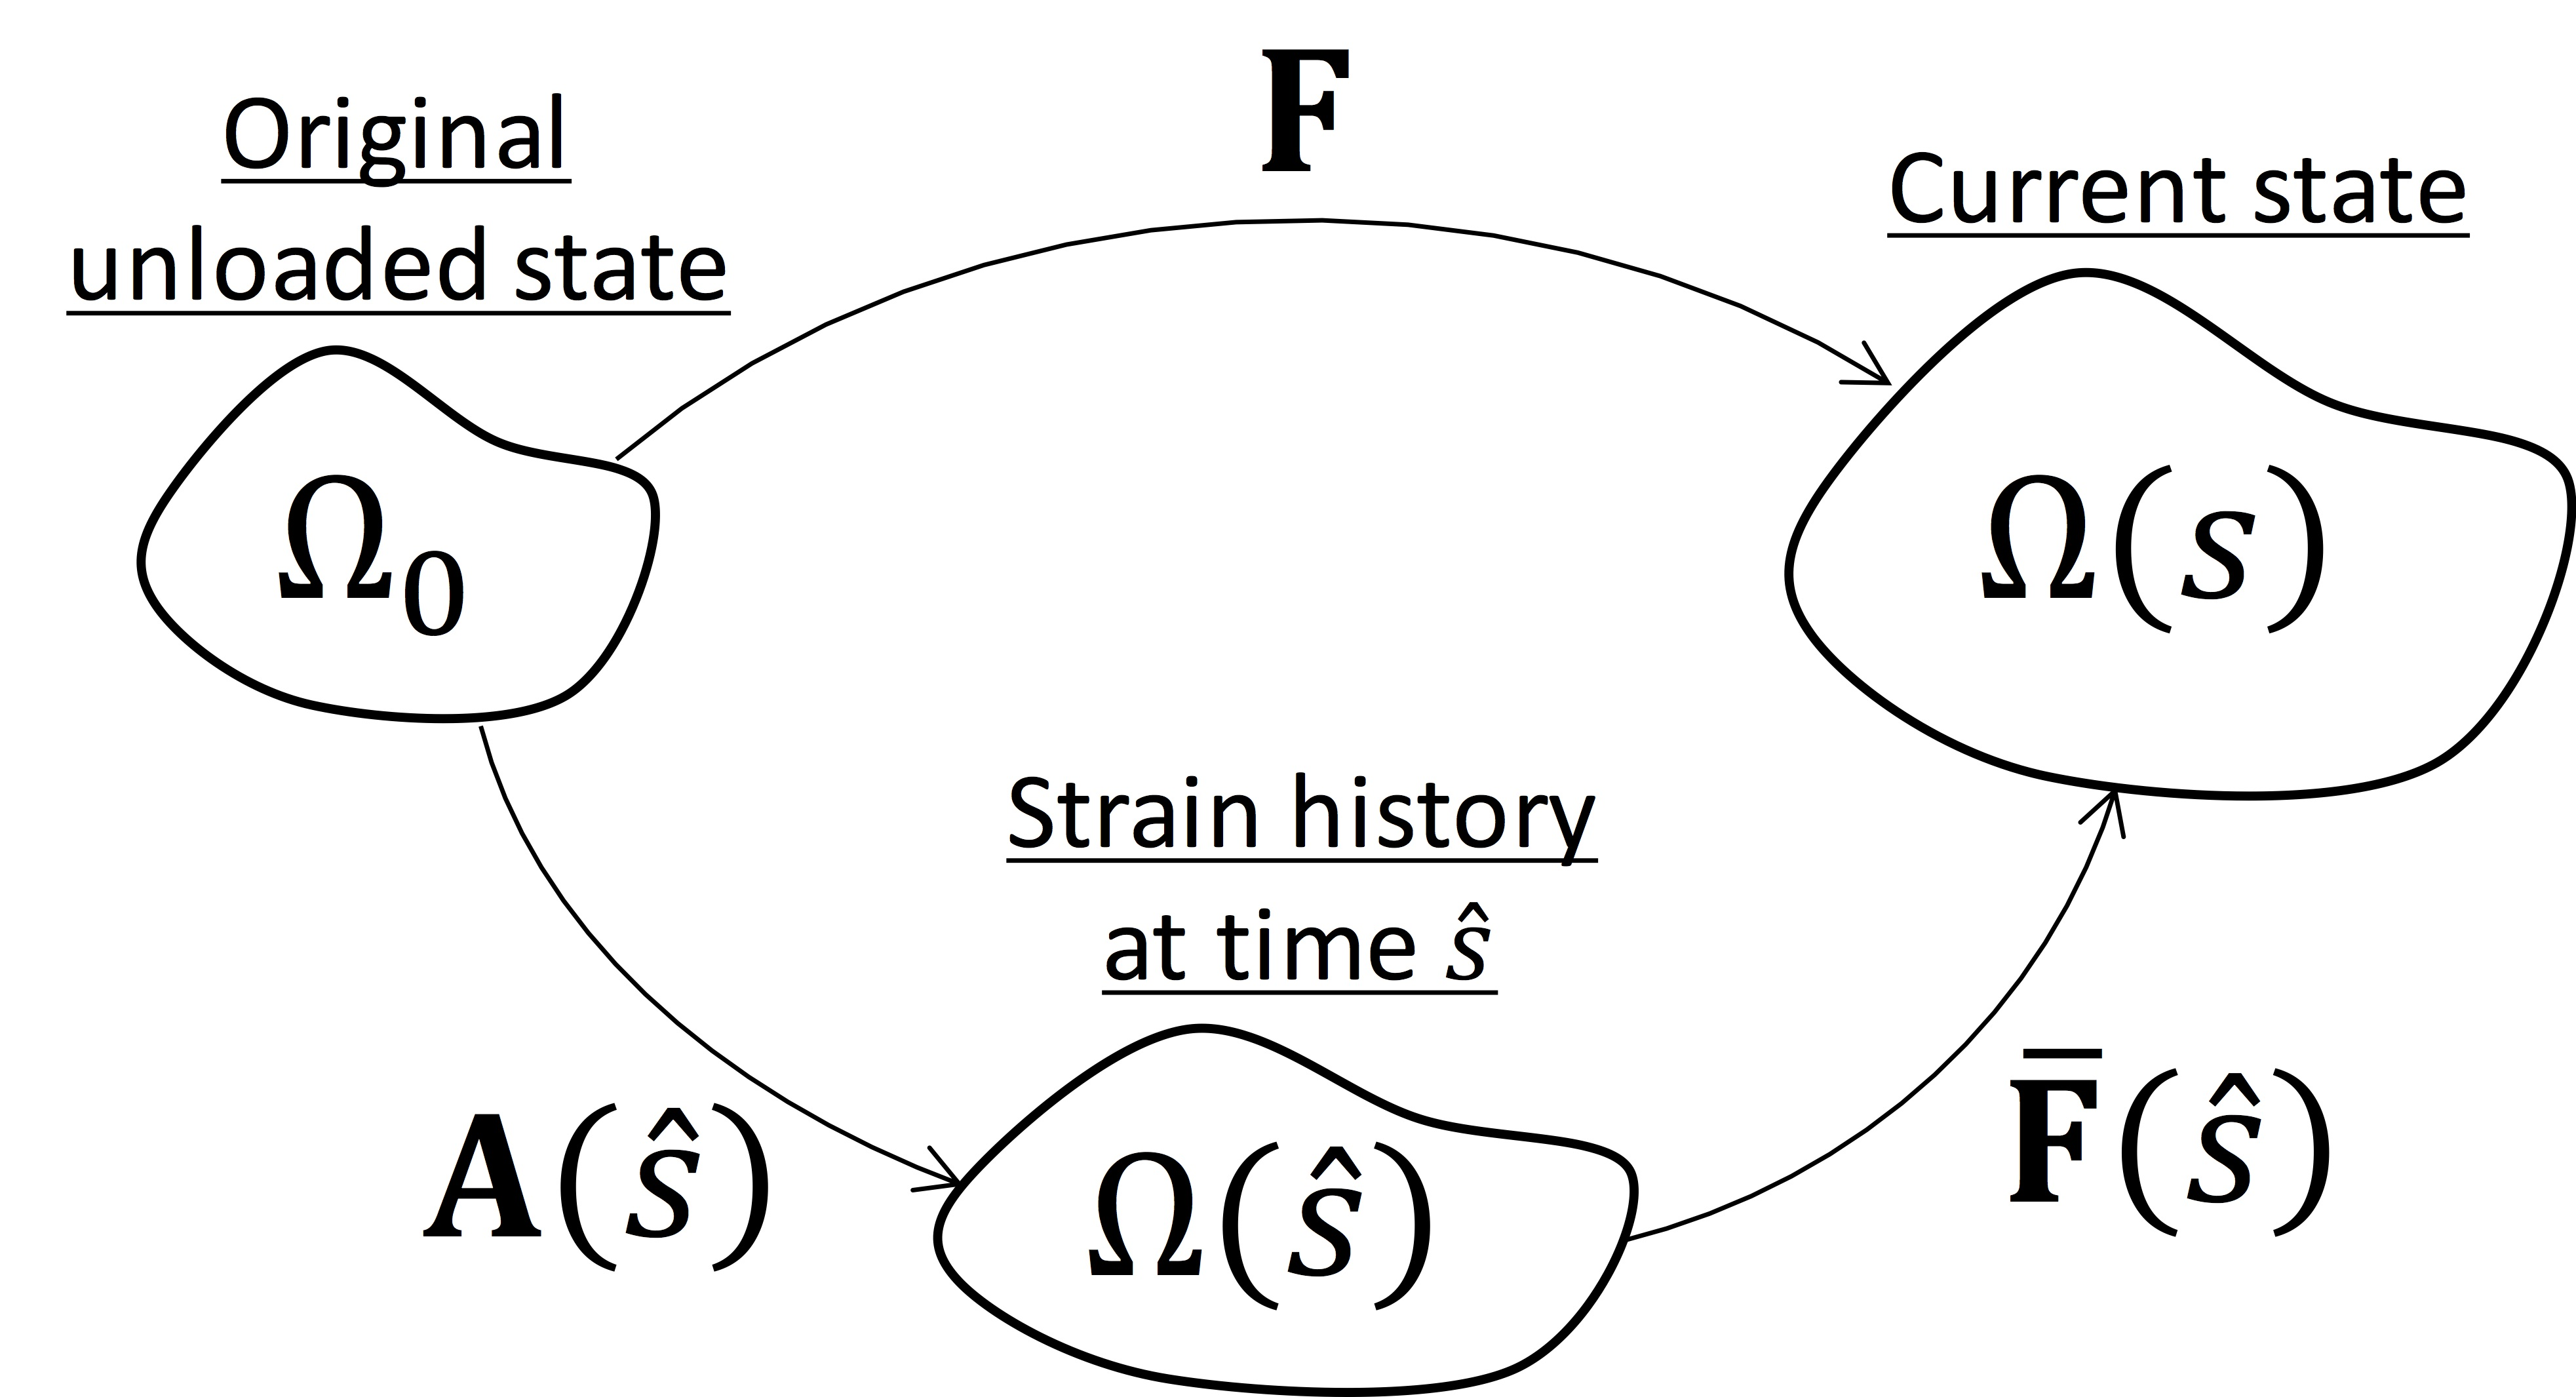
\includegraphics[width=3.5in]{Images/chapter4/figure7}
\caption{The relation between the reference configurations during cyclic loading.}
\label{fig:stateevolution}
\end{figure}

    We also note the following important considerations:
\begin{itemize}
\item The original reference configuration $\Omega_0$ is important as it is the configuration for which the mechanical response of the original material as well as the collagen fiber architecture is referenced. Similarly, we track the loaded configuration ($\Omega(s)$) using $\mathbf{A}(s)$ and the unloaded configuration ($\Omega_\mathrm{PS}(s)$) using $\mathbf{F}_\mathrm{PS}$ from $\Omega_0$. 

\item We also note that under cyclic loading, the exogenously crosslinked tissue is not held at the constant loaded configuration, it is put through a range of deformation each cycle. Because permanent set happens at a time scale much longer than a single cycle, we define the loaded configuration $\Omega(s)$ as the root mean squared configuration, which is the time averaged deformation for a single loading cycle. 

\item We note that the tissue is never fully unloaded during cyclic loading. Thus, to simulate cyclic loading, the stresses are still referenced to the origin configuration $\Omega_0$. The unloaded geometry is determined \textit{a posteriori} from $\Omega_\mathrm{PS}(s)$ for when cyclic loading is stopped for mechanical testing. 
\end{itemize}



    Thus the right Cauchy Green tensor when referenced to the strain history $\Omega(\hat{s})$ is given by $\mathbf{\bar{C}}(\hat{s}) = \mathbf{\bar{F}}(\hat{s})^\mathsf{T} \mathbf{\bar{F}}(\hat{s})$. This also has the following relation to the applied deformation $\mathbf{F}$,
\begin{equation} \label{eq:rightcauchy}
\begin{split}
\mathbf{\bar{C}}(\hat{s}) &= \left( \mathbf{F}\cdot\mathbf{A}(\hat{s})^{-1} \right)^\mathsf{T} \left(\mathbf{F} \cdot \mathbf{A}(\hat{s})^{-1} \right)\\
	&= \mathbf{A}(\hat{s})^{-\mathsf{T}} \left( \mathbf{F}^\mathsf{T} \mathbf{F} \right) \mathbf{A}(\hat{s})^{-1} \\
	&= \mathbf{A}(\hat{s})^{-\mathsf{T}} \cdot \mathbf{C} \cdot \mathbf{A}(\hat{s})^{-1}.
\end{split}
\end{equation}
    Our material model for the EXL matrix is an isotropic model of $\Psi_m = \Psi_m(I_1)$, where $I_1$ is the first invariant of $\mathbf{C}$. For this, we can define the first invariant $\bar{I}_1(\hat{s})$ for the right Cauchy Green tensor $\bar{\mathbf{C}}(\hat{s})$ as 
\begin{equation}\label{eq:pseudo1stinv}
\bar{I}_1(\hat{s}) = \operatorname{Trace}(\mathbf{\bar{C}}(\hat{s})) = \operatorname{Trace}\left(\mathbf{A}^{-\mathsf{T}}(\hat{s}) \cdot \mathbf{C} \cdot \mathbf{A}^{-1}(\hat{s})\right).
\end{equation}
    With this, the stress of the EXL matrix is given by 

\begin{equation}
\mathbf{\bar{S}}_m = 2 \frac{\partial \bar{\Psi}}{\partial \mathbf{C}} - p\mathbf{I} = 2 \frac{\partial \bar{\Psi}}{\partial \bar{I}_1(\hat{s})} \frac{\partial \bar{I}_1(\hat{s})}{\partial \mathbf{C}} - p\mathbf{I},
\end{equation}
    where $p$ is the Lagrange multiplier enforcing incompressibility. The partial derivative of $\bar{I}_1(\hat{s})$ is
\begin{equation}
\frac{\partial\bar{I}_1}{\partial\mathbf{C}} = \frac{\partial\bar{I}_1}{\partial\bar{\mathbf{C}}(\hat{s})} \frac{\partial\bar{\mathbf{C}}(\hat{s})}{\partial \mathbf{C}}= \frac{\partial\mathbf{A}(\hat{s})^{-\mathsf{T}} \cdot \mathbf{C} \cdot \mathbf{A}(\hat{s})^{-1}}{\partial \mathbf{C}} = \mathbf{A}(\hat{s})^{-\mathsf{T}} \mathbf{A}(\hat{s})^{-1} = \mathbf{\tilde{B}}(\mathbf{A}(\hat{s}))^{-1},
\end{equation}
    which is the inverse of the left Cauchy Green tensor of the strain history $\mathbf{A(s)}$.


%%%%%%%%%%%%%%%%%%%%%%%%%%%%%%%%%%%%%%%%%%%%%%%%%%%%%%%%%%%%
%%%%%%      Constitutive Model for crosslinking

\subsubsection{Kinematics for updating the reference configuration}

    As the unloaded configuration changes due to permanent set, we need to be able to express the stresses with the new reference configuration. Since all configurations are referenced to $\Omega_0$, the deformation from the new reference configuration $\Omega_\mathrm{PS}$ to the current loaded state $\Omega(s)$ is given by (Fig. \ref{fig:PSevolution})
\begin{equation}
\mathbf{F} = \mathbf{\bar{F}}(\hat{s}) \cdot \mathbf{A}(\hat{s}) \cdot \mathbf{F}_\mathrm{PS}^{-1}.
\end{equation}
    Following the same derivation as equations \ref{eq:strainhistory}--\ref{eq:pseudo1stinv}, we have
\begin{equation} \label{eq:newhistory}
\begin{split}
\mathbf{\bar{F}}(\hat{s}) &= \mathbf{F} \cdot \mathbf{F}_\mathrm{PS} \cdot \mathbf{A}(\hat{s})^{-1},\\
\mathbf{\bar{C}}(\mathbf{F}_\mathrm{PS}, \mathbf{A}(\hat{s})) &= \mathbf{A}(\hat{s})^{-\mathsf{T}} \cdot \mathbf{F}_\mathrm{PS}^\mathsf{T} \cdot \mathbf{C} \cdot \mathbf{F}_\mathrm{PS} \cdot \mathbf{A}(\hat{s})^{-1}, \\
\bar{I}_1\left(\mathbf{F}_\mathrm{PS}, \mathbf{A}(s)\right) &= \operatorname{Trace}\left(\mathbf{A}(\hat{s})^{-\mathsf{T}} \cdot \mathbf{F}_\mathrm{PS}^\mathsf{T} \cdot \mathbf{C} \cdot \mathbf{F}_\mathrm{PS} \cdot \mathbf{A}(\hat{s})^{-1}\right). 
\end{split}
\end{equation}
    and the new inverse of the left Cauchy Green tensor of the strain history is given by
\begin{equation}
\begin{split}
\mathbf{\tilde{B}}(\mathbf{F}_\mathrm{PS}, \mathbf{A}(\hat{s}))^{-1} &= \frac{\partial \mathbf{\bar{C}}(\mathbf{F}_\mathrm{PS}, \mathbf{A}(\hat{s}))}{\partial \mathbf{C}} = \frac{\mathbf{A}(\hat{s})^{-\mathsf{T}} \cdot \mathbf{F}_\mathrm{PS}^\mathsf{T} \cdot \mathbf{C} \cdot \mathbf{F}_\mathrm{PS} \cdot \mathbf{A}(\hat{s})^{-1}}{\partial \mathbf{C}} \\
 &= \mathbf{A}(\hat{s})^{-\mathsf{T}} \cdot \mathbf{F}_\mathrm{PS}^\mathsf{T} \cdot \mathbf{F}_\mathrm{PS} \cdot \mathbf{A}(\hat{s})^{-1}. 
\end{split}
\end{equation}

\begin{figure}[hbt]
\centering
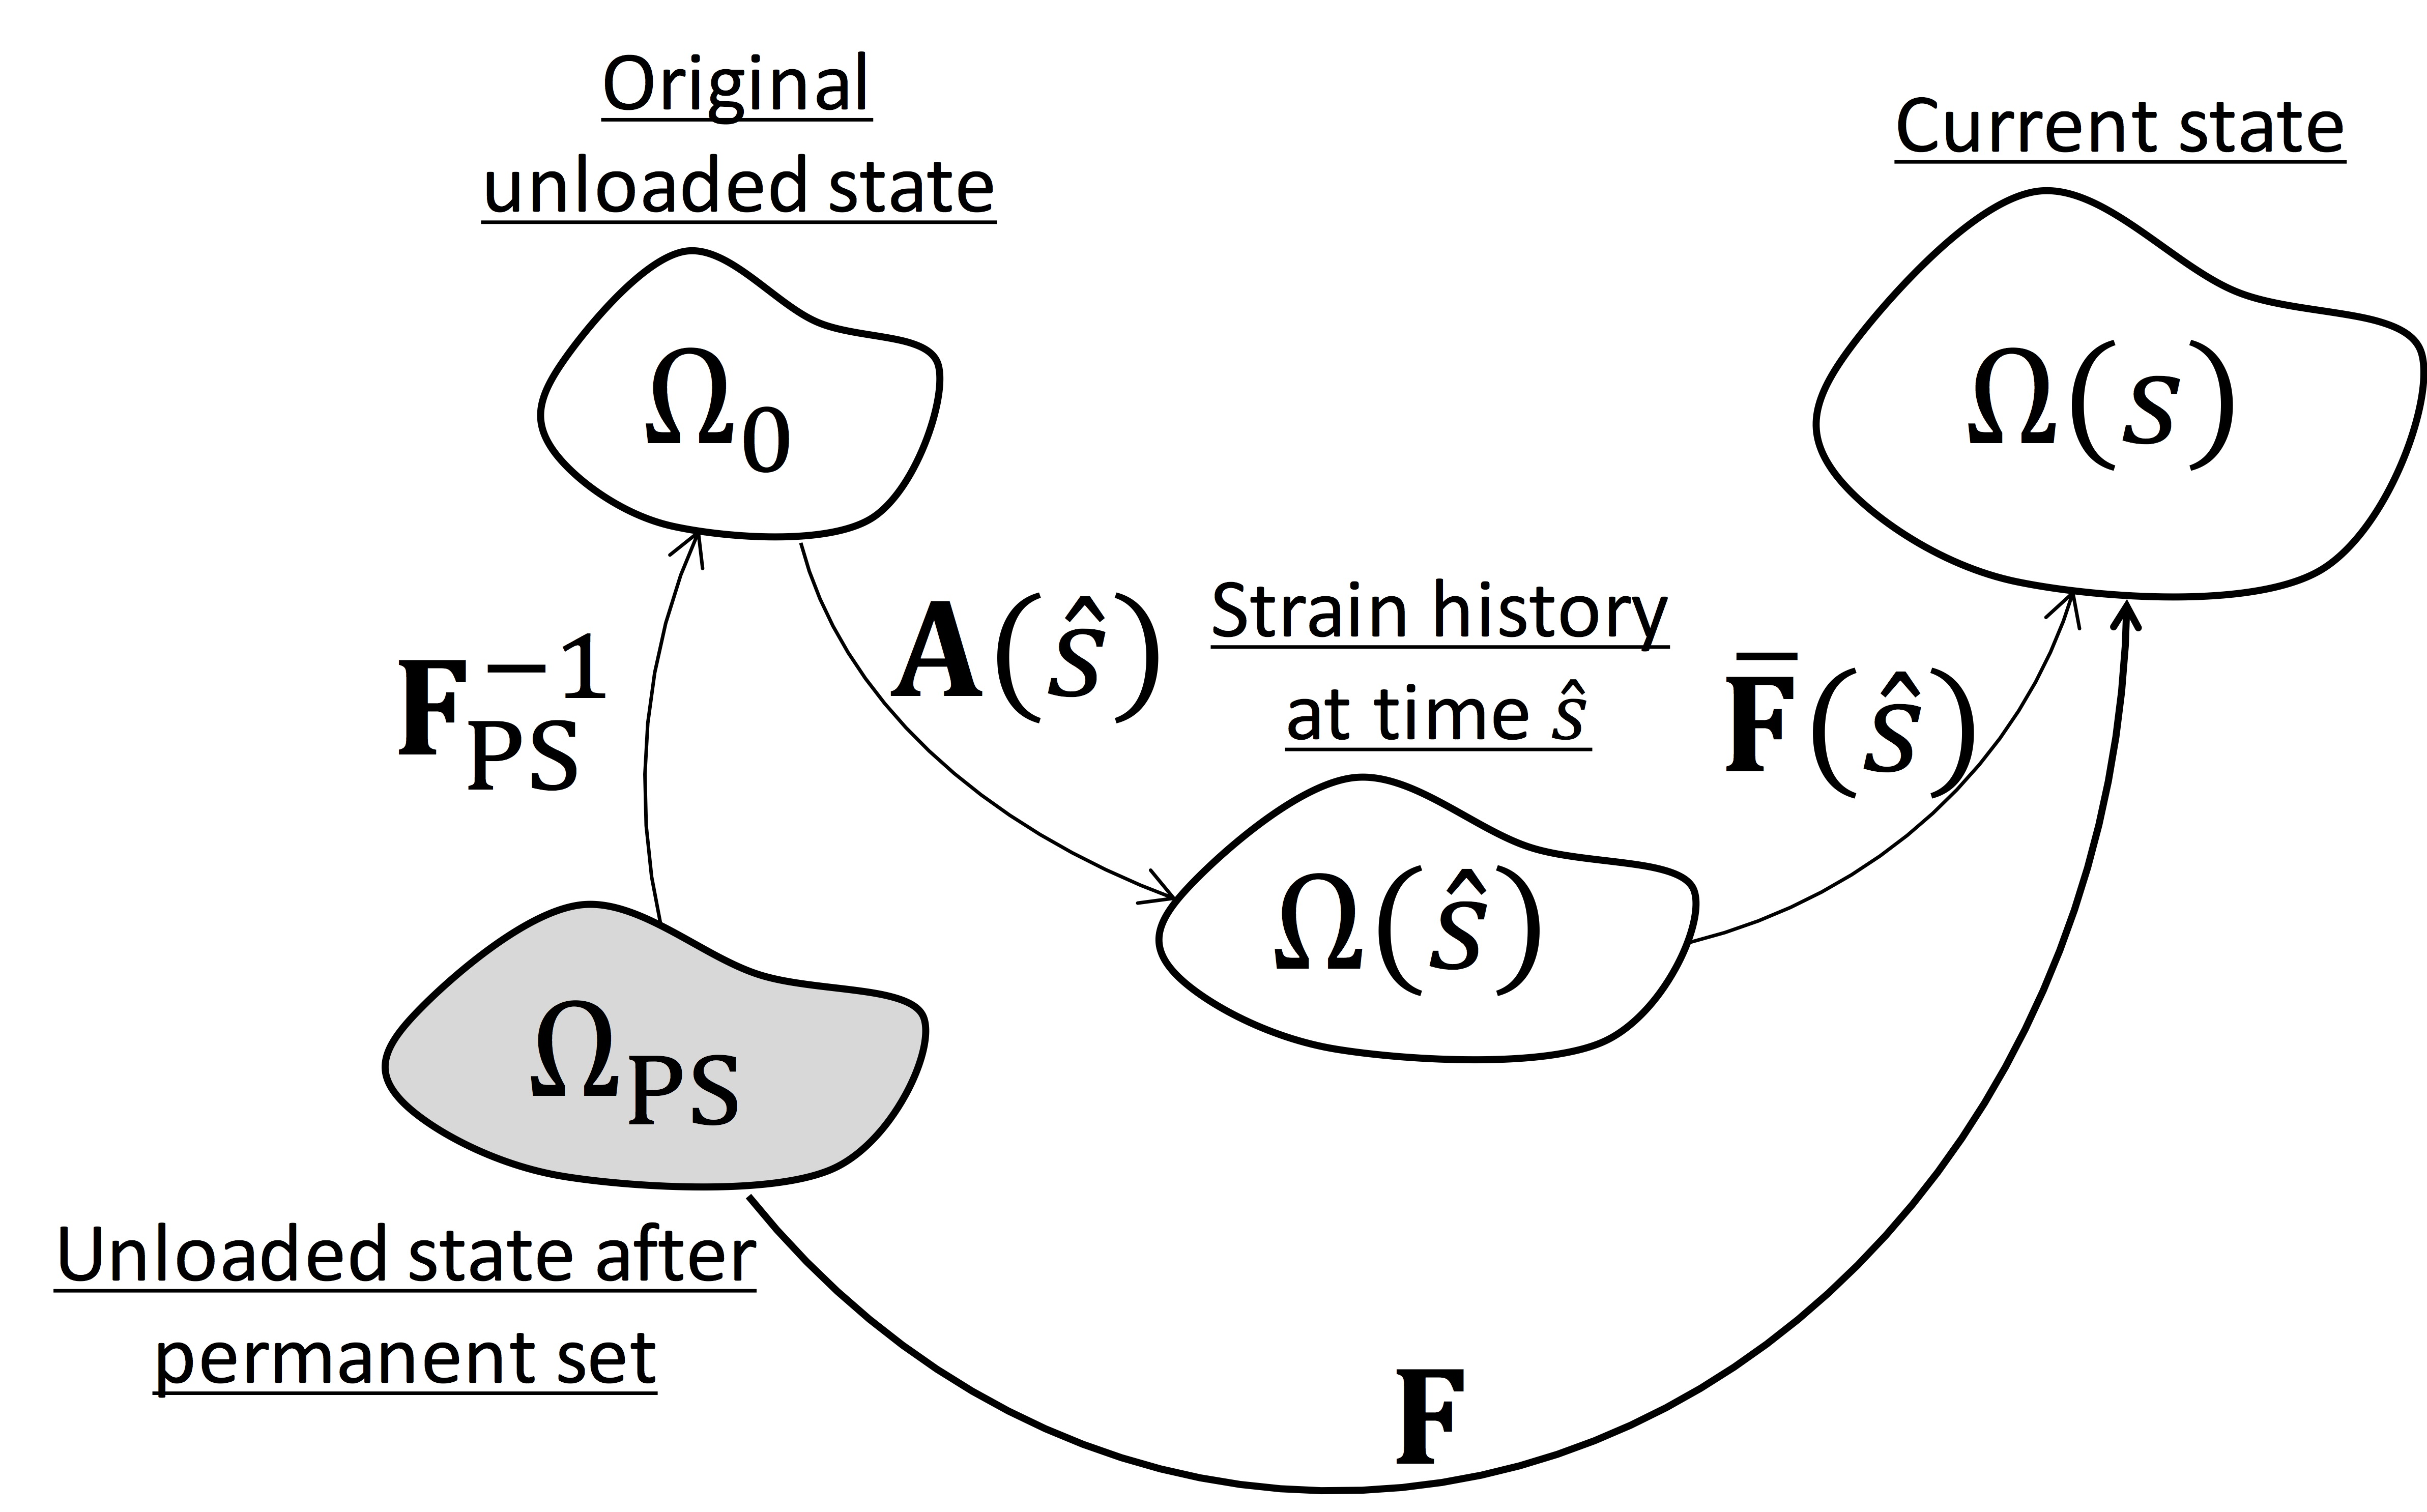
\includegraphics[width=4in]{Images/chapter4/figure8}
\caption{Modification of the relation between the different reference configurations when the unloaded configuration changes.}
\label{fig:PSevolution}
\end{figure}


%%%%%%%%%%%%%%%%%%%%%%%%%%%%%%%%%%%%%%%%%%%%%%%%%%%%%%%%%%%%%%%%%%%%%%%%%%%%%%%%
%%%%    Change in reference configuration

\subsection{Extension to the EXL matrix model for changes in reference configuration}

	We start by extending the EXL matrix model from our previous model \cite{sacks_novel_2016}. The strain energy is a modified form of the Yeoh model, which exhibits the following stress-strain relation,
\begin{equation}
\begin{split}
\Psi_m = &\frac{\eta_m}{2} \left( \frac{1}{\alpha}\left( I_1 -3\right)^{\alpha} + \frac{r}{\beta} \left( I_1 -3\right)^{\beta} \right), \\
&\text{with } 1<\alpha<\beta, \alpha\beta <2, 0 \leq r.
\end{split}
\end{equation}
    Here $\eta_m$ is the EXL matrix modulus, $\alpha,\beta$ are the exponent and $r$ is the relative weight between the two terms which is typically between 10 to 20. To modify the model form to reference the configuration at the time of formation $\Omega(\hat{s})$, we make the substitution for $\bar{I}_1(\mathbf{F}_\mathrm{PS}, \mathbf{A}(\hat{s}))$ (Eqn. \ref{eq:pseudo1stinv}),
\begin{equation} \label{eq:matrixenergyform}
\bar{\Psi}_m\left( \mathbf{C}, \mathbf{A}(\hat{s})\right) = \frac{\eta_m}{2} \left(\frac{1}{\alpha} \left( \bar{I}_1\left(\mathbf{F}_\mathrm{PS}, \mathbf{A}(s)\right) -3\right)^\alpha +\frac{r}{\beta} \left( \bar{I}_1\left(\mathbf{F}_\mathrm{PS}, \mathbf{A}(s)\right) -3\right)^\beta \right),
\end{equation}
    The derivative of the strain energy with respect to the invariant $\bar{I}_1$ is 
\begin{equation}
\frac{\partial \bar{\Psi}}{\partial \bar{I}_1} =	\frac{\eta_m}{2} \left(\left( \bar{I}_1\left(\mathbf{F}_\mathrm{PS}, \mathbf{A}(s)\right)- 3\right)^{\alpha - 1} + r \left( \bar{I}_1\left(\mathbf{F}_\mathrm{PS}, \mathbf{A}(s)\right) - 3\right)^{\beta - 1}\right).
\end{equation}
    After solving for the Lagrange multiplier $p$, with $\bar{S}_{m,33} = 0$, we have 
\begin{equation}\label{eq:matrixfinal}
\begin{split}
\mathbf{\bar{S}}_m \left( \mathbf{F}_\mathrm{PS},\mathbf{A}(\hat{s}),\mathbf{C}\right) &= \mu_m \left(\left( \bar{I}_1\left(\mathbf{F}_\mathrm{PS}, \mathbf{A}(s)\right) - 3\right)^{\alpha - 1} + r \left( \bar{I}_1\left(\mathbf{F}_\mathrm{PS}, \mathbf{A}(s)\right) - 3\right)^{\beta - 1}\right) \\
&\times \left( \mathbf{\tilde{B}}(\mathbf{F}_\mathrm{PS}, \mathbf{A}(\hat{s}))^{-1} - \tilde{B}_{33}^{-1}(\mathbf{F}_\mathrm{PS}, \mathbf{A}(\hat{s}))C_{33}\mathbf{C}^{-1}\right).
\end{split}
\end{equation}


%%%%%%%%%%%%%%%%%%%%%%%%%%%%%%%%%%%%%%%%%%%%%%%%%%%%%%%%%%%%
%%%%%%      Extension for permanent set

\subsubsection{Extension of the EXL matrix for the permanent set effect}

	Next, we developed the model form for the EXL matrix after permanent set. This approach is based on the work by Rajagopal and Wineman \cite{rajagopal_constitutive_1992}, where we assume that the response of the full EXL matrix to be 
\begin{equation} \label{eq:wineman}
\phi_m \mathbf{S}_m = b(s)\mathbf{\bar{S}}_m^\mathrm{existing} + \int\displaylimits_0^s a(s,\hat{s})\mathbf{\bar{S}}_m^\mathrm{new} \mathrm{d}\hat{s},
\end{equation}
    where $b(s)$ is the remaining amount of the existing material, $a(s,\hat{s})$ is the remaining amount of the new material formed during the strain history ($\mathbf{A}(s)$) at time $\hat{s}$, $\mathbf{\bar{S}}_m^\mathrm{existing}$ is the stress of the existing material and $\mathbf{\bar{S}}_m^\mathrm{new}$ is the stress of the new material. Assuming first order kinetics with the permanent set rate constant $k $, we have for the material remaining (Fig. \ref{fig:masstransfer})
\begin{equation}
\frac{\partial b(s)}{\partial s} = - k\cdot b(s), \qquad \frac{\partial a(s,\hat{s})}{\partial s} = - k \cdot a(s,\hat{s}).
\end{equation}
    Given that the total amount of EXL matrix ($\phi_m$) has not changed, $b(s) + \int_0^s a(s, \hat{s}) \mathrm{d}\hat{s} = \phi_m$, and we have
\begin{equation}
b(s) = \phi_m \mathrm{Exp}\left[-k  \cdot s\right], \qquad a(s,\hat{s}) = \phi_m k  \mathrm{Exp}\left[-k (s - \hat{s})\right].
\end{equation}
    Substitution into equation \ref{eq:wineman}, we have the mechanical response of the EXL matrix after permanent set,
\begin{equation}
\phi_m \mathbf{S}_m = \phi_m \left[\mathrm{Exp}\left[-k  \cdot s\right]\mathbf{\bar{S}}_m \left(\mathbf{F}_\mathrm{PS},\mathbf{A}(0),\mathbf{C}\right) + \int\displaylimits_0^s k \cdot \mathrm{Exp}\left[-k (s - \hat{s})\right] \mathbf{\bar{S}}_m \left(\mathbf{F}_\mathrm{PS},  \mathbf{A}(\hat{s}),\mathbf{C}\right) \mathrm{d}\hat{s} \right].
\end{equation}
    The final form for the EXL matrix component of the permanent set model is thus,
\begin{equation}
\begin{split}
\phi_m \mathbf{S}_m \left(\mathbf{F}_\mathrm{PS}, \mathbf{A}(\hat{s}),\mathbf{C}\right) &= \phi_m \mu_m \left[ \vphantom{\int\displaylimits_0^s} \mathrm{Exp}\left[-k  \cdot s\right]  \left(\left( \bar{I_1} (\mathbf{F}_\mathrm{PS}, \mathbf{A}(0)) - 3\right)^{\alpha - 1} + r \left( \bar{I_1} (\mathbf{F}_\mathrm{PS}, \mathbf{A}(0)) - 3\right)^{\beta - 1}\right)  \right.\\
&\times \left( \mathbf{\tilde{B}}(\mathbf{F}_\mathrm{PS}, \mathbf{A}(0))^{-1} - \tilde{B}_{33}(\mathbf{F}_\mathrm{PS}, \mathbf{A}(0))^{-1}C_{33}\mathbf{C}^{-1}\right) \\
&+ \int\displaylimits_0^s k \cdot \mathrm{Exp}\left[-k (s - \hat{s})\right] \left(\left( \bar{I_1} (\mathbf{F}_\mathrm{PS}, \mathbf{A}(\hat{s})) - 3\right)^{\alpha - 1} + r \left( \bar{I_1} (\mathbf{F}_\mathrm{PS}, \mathbf{A}(\hat{s})) - 3\right)^{\beta - 1}\right) \\
&\times \left. \vphantom{\int\displaylimits_-^s} \left( \mathbf{\tilde{B}}(\mathbf{F}_\mathrm{PS}, \mathbf{A}(\hat{s}))^{-1} - \tilde{B}_{33}(\mathbf{F}_\mathrm{PS}, \mathbf{A}(\hat{s}))^{-1}C_{33}\mathbf{C}^{-1}\right) \mathrm{d}\hat{s}\right].
\end{split}
\end{equation}

\begin{figure}[hbt]
\centering
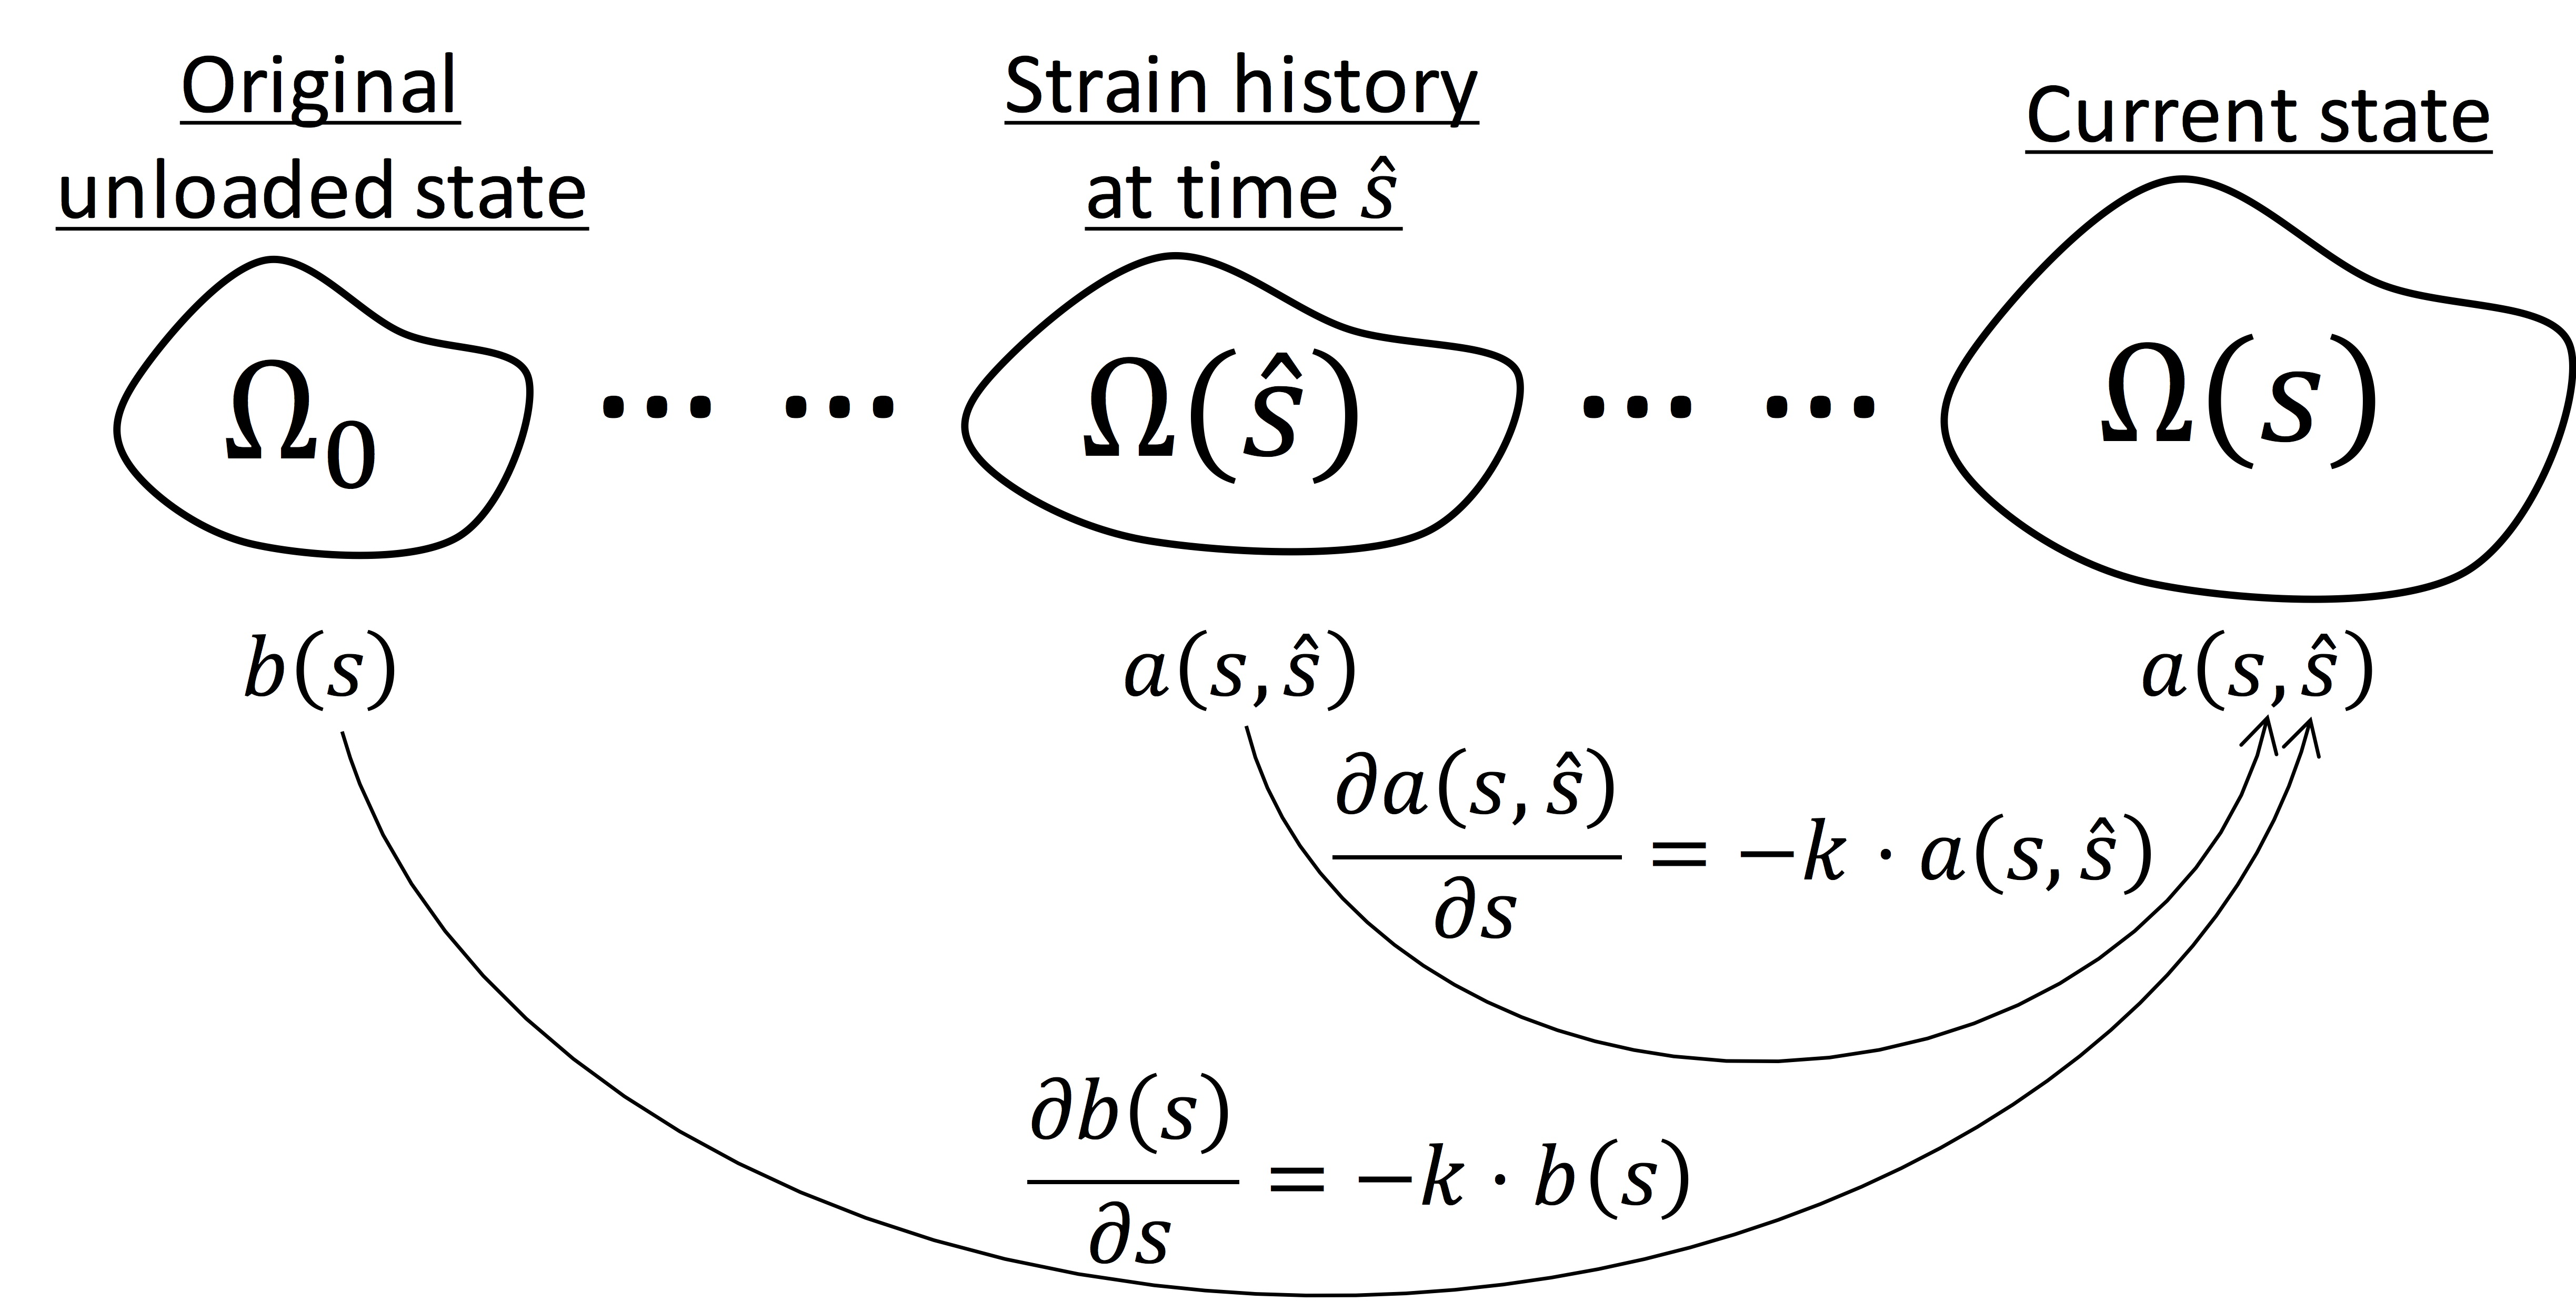
\includegraphics[width=4.5in]{Images/chapter4/figure9}
\caption{The mass fractions of the EXL matrix change over time, assuming first order kinetics. }
\label{fig:masstransfer}
\end{figure}

%%%%%%%%%%%%%%%%%%%%%%%%%%%%%%%%%%%%%%%%%%%%%%%%%%%%%%%%%%%%%%%%%%%%%%%%%%%%%%%%
%%%%    Structural Convection

\subsection{Convection of the collagen fiber architecture} \label{sec:convection}

    Now that the model form for the EXL matrix under permanent set is established, we need to consider how the collagen fiber architecture is convected by the change in reference configuration. The convection of the collagen fiber architecture is done through two parts: the ODF and the recruitment function. This is done by assuming that the collagen fiber architecture is convected under the affine assumption\cite{lee_presence_2015}. The form of the ODF and the recruitment distribution was previously described in Zhang \textit{et al.} \cite{zhang_meso_2016}, and the operation used to convect the collagen fiber architecture is given in Sacks \textit{et al}. \cite{sacks_novel_2016}. Briefly, the convected ODF $\Gamma_1$ is determined from the ODF in the 0-cycle state $\Gamma_0$ and the deformation $\prescript{1}{0}{\mathbf{F}}$ by the conservation of the number of fiber $\Gamma(\theta_0) \mathrm{d}\theta_0 = \Gamma(\theta_1) \mathrm{d}\theta_1$ (Fig. \ref{fig:effectsofconvection}A). This is given by
\begin{equation} \label{eq:pfODF}
\begin{gathered}
\Gamma_1\left( \prescript{1}{0}{\mathbf{F}},\theta_1 \right) = \Gamma_0\left( \theta_0\left( \prescript{1}{0}{\mathbf{F}},\theta_1\right)\right)\frac{\prescript{1}{0}{\lambda(\theta_0)}^2}{\prescript{1}{0}{J_\mathrm{2D}}}, \\
\prescript{1}{0}{\lambda(\theta_0)} = \sqrt{\mathbf{n}_{\theta_0}\cdot  \prescript{1}{0}{\mathbf{F}^\mathsf{T}}  \prescript{1}{0}{\mathbf{F}} \cdot \mathbf{n}_{\theta_0}}, \qquad \prescript{1}{0}{J_\mathrm{2D}} =\det (\prescript{1}{0}{\mathbf{F}}),
\end{gathered}
\end{equation}
    where $\mathbf{n}_\theta$ is a unit vector for the orientation $\theta$. The distribution of slack stretch needed to straighten collagen fiber crimp after convection, in other words the recruitment distribution $D_1(\lambda_s)$ (Fig. \ref{fig:effectsofconvection}B), is given by
\begin{equation} \label{eq:pfrecruitment}
\begin{gathered}
D_1(\prescript{1}{0}{\mathbf{F}}, \lambda_s) = \begin{cases} \frac{\operatorname{B}[\gamma_0,\gamma_1](y)}{\prescript{}{1}{\lambda}_\mathrm{ub}-\prescript{}{1}{\lambda}_\mathrm{lb}} & \prescript{}{1}{\lambda}_\mathrm{ub} < y < \prescript{}{1}{\lambda}_\mathrm{lb} \\ 0 & \text{else}\end{cases}, \\
\qquad \prescript{}{1}{\lambda}_s = \frac{\lambda_s}{\prescript{1}{0}{\lambda}(\theta)}, \qquad y = \frac{\prescript{}{1}{\lambda}_s - \prescript{}{1}{\lambda}_\mathrm{lb}}{\prescript{}{1}{\lambda}_\mathrm{ub}-\prescript{}{1}{\lambda}_\mathrm{lb}}.
\end{gathered}
\end{equation}
where $\prescript{1}{0}{\lambda(\theta_0)}$ is defined in equation \ref{eq:pfODF}, $(\prescript{}{1}{\lambda}_\mathrm{lb},\prescript{}{1}{\lambda}_\mathrm{ub})$ are the new bounds of the distribution after being convected, and $(\gamma_0,\gamma_1)$ are the shape parameters of the beta distribution function $B$ .
The model form for collagen fibers in exogenously crosslinked BP after being convected by a change in geometry is previously presented in Sacks et al. \cite{sacks_novel_2016} and can also be used for the convection of the collagen fiber architecture due to the permanent set effect. 
The model form for the fiber ensemble interactions is given by equation \ref{eq:interaction}, where equations \ref{eq:pfODF} and \ref{eq:pfrecruitment} are substituted in for the ODF and recruitment distribution function for the mechanical response after permanent set.


\begin{figure}[hbt]
\centering
\centerline{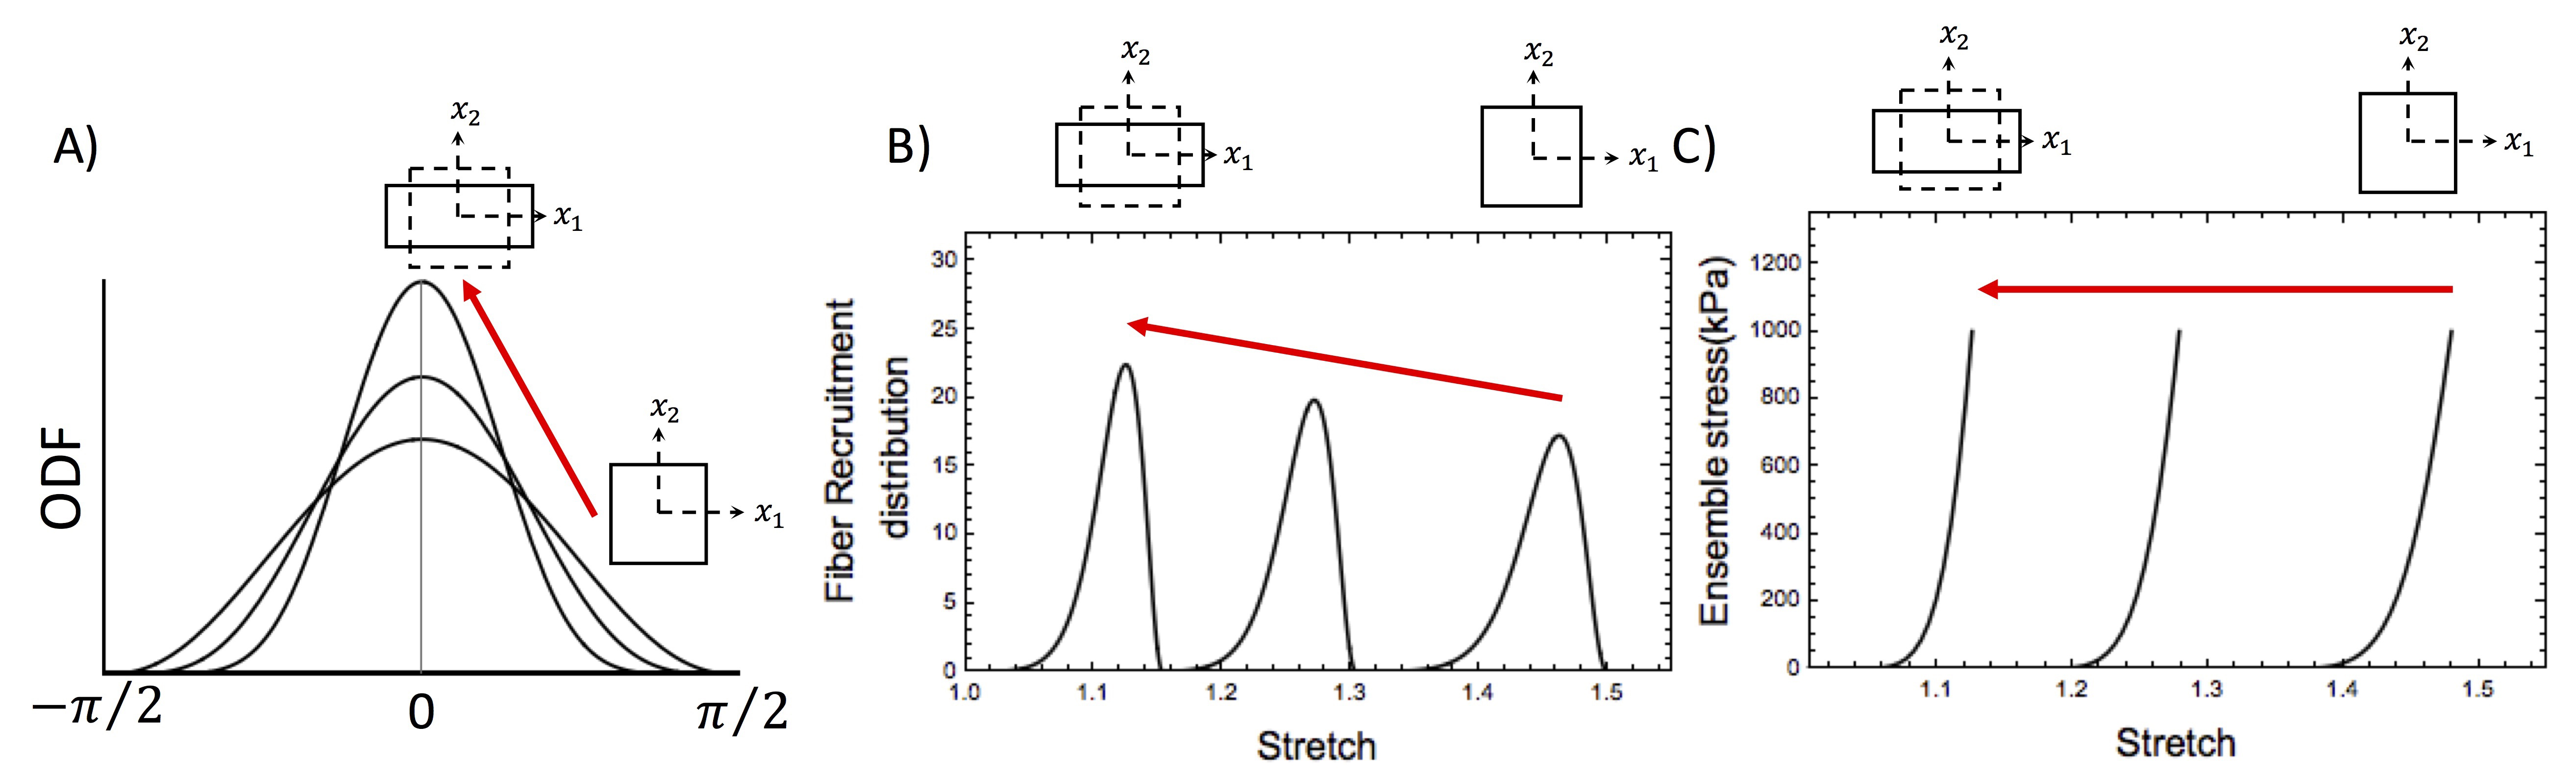
\includegraphics[width=\textwidth]{Images/chapter4/figure10}}
\caption{The effects of convecting the collagen fiber architecture show A) gradual alignment of collagen fibers, B) changes in the probability distribution of collagen fiber lack stretches and C) its effect on the mechanical response.}
\label{fig:effectsofconvection}
\end{figure}



%%%%%%%%%%%%%%%%%%%%%%%%%%%%%%%%%%%%%%%%%%%%%%%%%%%%%%%%%%%%%%%%%%%%%%%%%%%%%%%%
%%%%    Further considerations

\subsection{Further considerations of the permanent set mechanism.}

	In addition to the above considerations, we explored the the following as a means to validate the mechanisms we proposed for permanent set. This was done by performing an analysis on predicting the mechanical response after cyclic loading using only the convection of the collagen fiber architecture by the measured $\textbf{F}_{PS}$. The analysis takes the following steps: 1) Material model parameter estimation for the 0-cycle data for the strain controlled data. This is done using the approach from Sacks \textit{et al}.\cite{sacks_novel_2016}, with the constitutive model for collagen fibers and the EXL matrix from the same study, and the interaction model from equation \ref{eq:interaction}. 
	2) Use equations \ref{eq:pfODF} and \ref{eq:pfrecruitment} (Sec.\ref{sec:convection}) to convect the collagen fiber architecture (Fig. \ref{fig:structuralconvection} and Fig. \ref{fig:effectsofconvection}). 
	The deformation used to convect the collagen fiber architecture is determined from the fiducial markers. 
	3) We compare the new convected exogenously crosslinked mechanical response to the experimental data.

%\subsection{Mechanical response predicted from convected collagen fiber architecture vs experimental data after cycling}

	We used this approach to examine both the strain (n = 3) and stress controlled specimens (n = 5), and tested the hypothesis that \emph{there is a significant different between the mechanical response predicted from structural convection and the experimentally measure data}, in other words, our model is not sufficient to explain the change in mechanical response. We take the maximum stress of each specimen under equibiaxial strain, and compared the difference between the model and the experimental data using student t-test.	For the strain control specimens, we found that there is no statistical significant difference between the convected mechanical response and the experimental data, where the average p-value of the PD and XD for both after 30 million cycle and after 65 million cycle is $p = 0.37$ (minimum $p > 0.07$). 
	Likewise, we also found no statistical significant differences between the convected response and the experimental data for the stress controlled specimens, where the average p-value is 0.57 (Fig. \ref{fig:mechconvec}).
	These results suggest that 1) the underlying collagen fiber architecture, including collagen fiber crimp and orientation, is convected affinely according to the permanent set in the EXL matrix. This indicates that our approach to model permanent set is realistic, and the underlying mechanism for permanent set is likely to be correct. 
	2) Structural damage to the collagen fiber architecture was not detectable at this stage (up to 65 million cycles). 
	These important results indicate that permanent set alone is sufficient to capture the response to cyclic loading up to 50-65 million cycles. 


\begin{figure}[hbt]
\centering
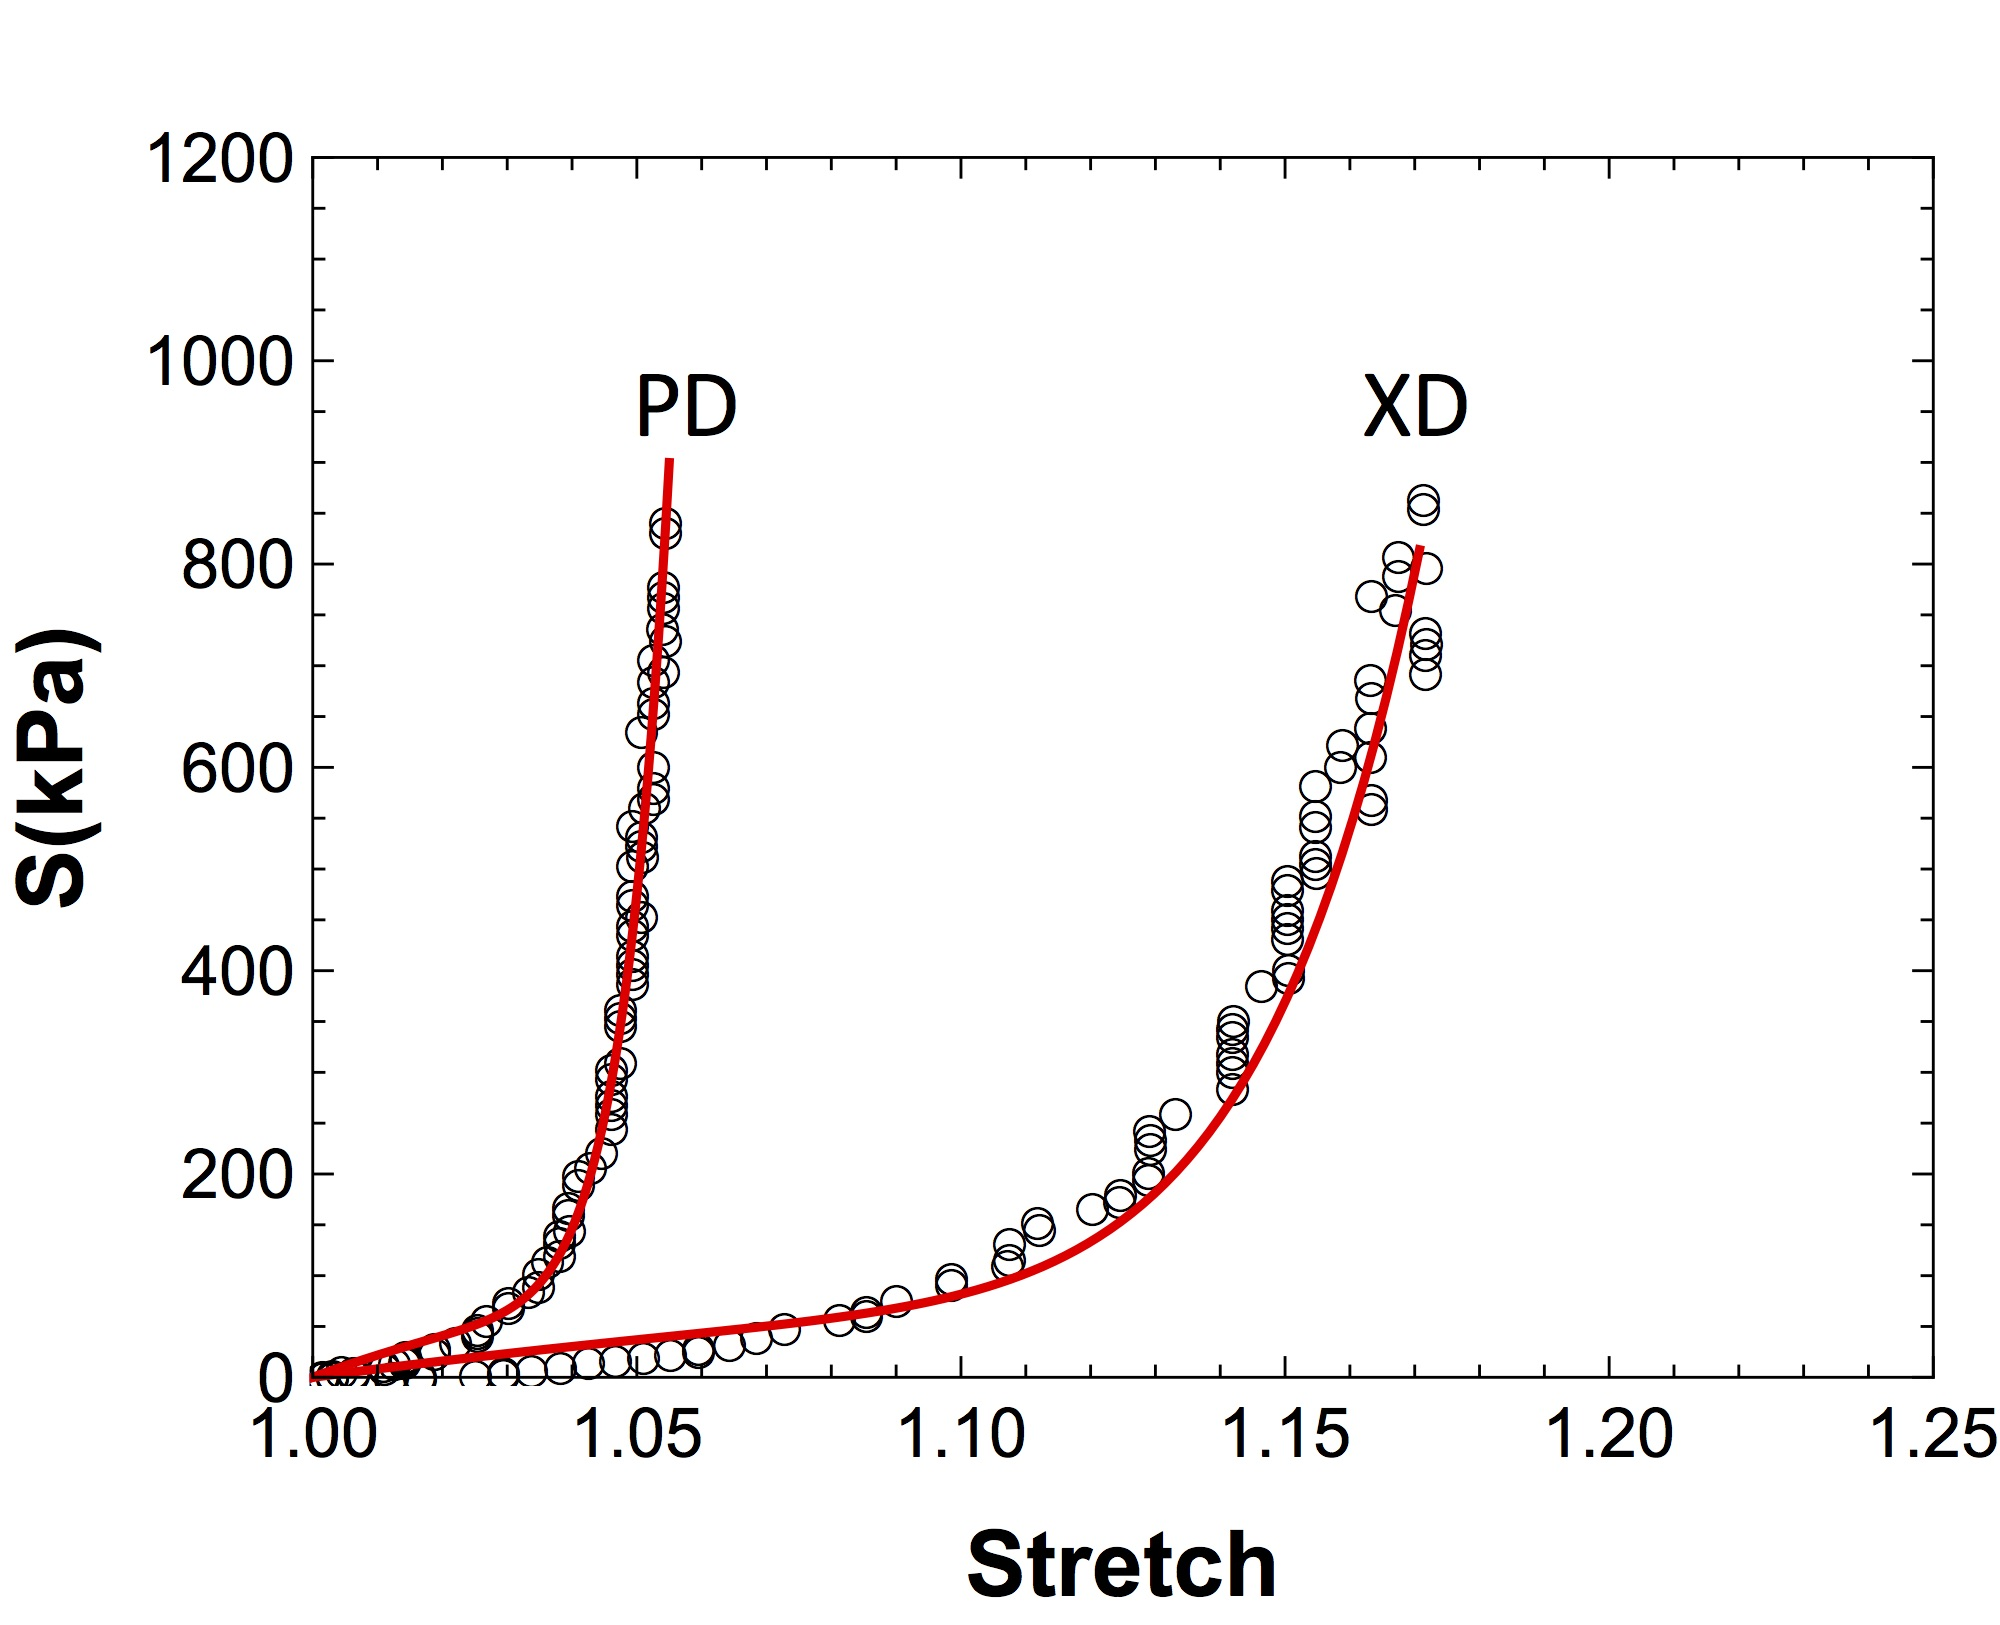
\includegraphics[width=3.5in]{Images/chapter4/figure11}
\caption{The equibiaxial mechanical response of an exogenously crosslinked BP specimen after 50 million cycles and the mechanical response determined from structural convection (Red) using the measured $\textbf{F}_{PS}$}
\label{fig:mechconvec}
\end{figure}


%%%%%%%%%%%%%%%%%%%%%%%%%%%%%%%%%%%%%%%%%%%%%%%%%%%%%%%%%%%%%%%%%%%%%%%%%%%%%%%%
%%%%    Full model form

\subsection{Full model form}
	Combining all three components, we have the final model form as a function of the permanent set rate constant $k $, the permanent set deformation $\mathbf{F}_\mathrm{PS}$, the strain history $\mathbf{A}(s)$, and the material parameters of the constitutive model in the uncycled state. The input of the model is the applied deformation $\mathbf{C}$ referenced to the current unloaded state $\Omega_\mathrm{PS}$, given by the deformation $\mathbf{F}_\mathrm{PS}$ from $\Omega_0$. The full form is
\begin{equation}\label{eq:fullEXLmodel}
\mathbf{S} = \mathbf{S}\left(k , \mathbf{F}_\mathrm{PS}, \mathbf{A}(\hat{s}), \mathbf{C}\right) = \phi_\mathrm{col} \left[ \mathbf{S}_\mathrm{col} + \mathbf{S}_\mathrm{int}\right] + \phi_m \mathbf{S}_\mathrm{m},
\end{equation}
where the collagen contribution is 
\begin{equation} \label{eq:fullcollagen}
\begin{split}
\phi_\mathrm{col}\mathbf{S}_\mathrm{col}\left(k , \mathbf{F}_\mathrm{PS}, \mathbf{A}(\hat{s}), \mathbf{C}\right) =& \phi_\mathrm{col} \eta_C \int\displaylimits_\theta \Gamma_1(\mathbf{F}_{\mathrm{PS}}, \theta)\left\lbrace 
\int\displaylimits_1^{\lambda_\theta} \frac{D_1\left( \mathbf{F}_{\mathrm{PS}}, x \right)}{x} \left( \frac{1}{x}- \frac{1}{\lambda_\theta}\right) \mathrm{d}x \right\rbrace \mathbf{n}_\theta\otimes\mathbf{n}_\theta \mathrm{d}\theta,
\end{split}
\end{equation}
where $\lambda_\theta = \sqrt{\mathbf{n}_\theta \cdot \mathbf{C}\mathbf{n}_\theta}$ is the stretch of the fiber ensemble oriented along $\theta$, the fiber ensemble interactions is 
\begin{equation} \label{eq:fullinteractions}
\begin{split}
\phi_\mathrm{int}\mathbf{S}_\mathrm{int}\left(k , \mathbf{F}_\mathrm{PS}, \mathbf{A}(\hat{s}), \mathbf{C}\right) = \phi_\mathrm{col} \eta_\mathrm{int}& \int\displaylimits_\alpha \int\displaylimits_\beta \Gamma_1 \left(\mathbf{F}_\mathrm{PS}, \alpha \right) \Gamma_1 \left(\mathbf{F}_\mathrm{PS},  \beta \right) \\
\times&\left[ \left\lbrace 
\int\displaylimits_1^{\lambda_\alpha} \int\displaylimits_1^{\lambda_\beta} 
\frac{2 \lambda_\beta D_1(\mathbf{F}_\mathrm{PS}, x_\alpha) D_1(\mathbf{F}_\mathrm{PS}, x_\beta)}{x_\alpha x_\beta} 
\left( \frac{\lambda_\alpha}{x_\alpha} \frac{\lambda_\beta}{x_\beta} - 1\right) \mathrm{d}x_\alpha \, \mathrm{d}x_\beta \right.\right. \\
+& \left. \left. \int\displaylimits_1^{\lambda_\beta} D_1(\mathbf{F}_\mathrm{PS}, x_\beta) \left( \frac{\lambda_\beta}{x_\beta} -1  \right)^2 \mathrm{d}x_\beta \right\rbrace \right.  \frac{\mathbf{n}_\alpha \otimes \mathbf{n}_\alpha}{\lambda_\alpha}  \\
+& \left. \left\lbrace
\int\displaylimits_1^{\lambda_\alpha} \int\displaylimits_1^{\lambda_\alpha} 
\frac{2 \lambda_\beta D_1(\mathbf{F}_\mathrm{PS}, x_\alpha) D_1(\mathbf{F}_\mathrm{PS}, x_\beta)}{x_\alpha x_\beta} 
\left( \frac{\lambda_\alpha}{x_\alpha} \frac{\lambda_\beta}{x_\beta} - 1\right) \mathrm{d}x_\alpha \, \mathrm{d}x_\beta 
\right. \right. \\
+&\left. \left. \int\displaylimits_1^{\lambda_\alpha} D_1(\mathbf{F}_\mathrm{PS}, x_\alpha) \left( \frac{\lambda_\alpha}{x_\alpha} -1  \right)^2 \mathrm{d}x_\alpha \right\rbrace \frac{\mathbf{n}_\beta \otimes \mathbf{n}_\beta}{\lambda_\beta}  \right] \mathrm{d}\alpha \, \mathrm{d}\beta,
\end{split}
\end{equation}
and the EXL matrix is
\begin{equation} \label{eq:fullmatrix}
\begin{split}
\phi_m \mathbf{S}_\mathrm{m}\left(k , \mathbf{F}_\mathrm{PS}, \mathbf{A}(\hat{s}), \mathbf{C}\right) = \phi_m \eta_m& \left[ \vphantom{\int\displaylimits_0^s} \mathrm{Exp}\left[-k  \cdot s\right]  \left(\left( \bar{I_1} (\mathbf{F}_\mathrm{PS}, \mathbf{A}(0)) - 3\right)^{\alpha - 1} + r \left( \bar{I_1} (\mathbf{F}_\mathrm{PS}, \mathbf{A}(0)) - 3\right)^{\beta - 1}\right)  \right.\\
\times& \left( \mathbf{\tilde{B}}(\mathbf{F}_\mathrm{PS}, \mathbf{A}(0))^{-1} - \tilde{B}_{33}^{-1}(\mathbf{F}_\mathrm{PS}, \mathbf{A}(0))C_{33}\mathbf{C}^{-1}\right) \\
+& \int\displaylimits_0^s k \cdot \mathrm{Exp}\left[-k (s - \hat{s})\right] \left(\left( \bar{I_1} (\mathbf{F}_\mathrm{PS}, \mathbf{A}(\hat{s})) - 3\right)^{\alpha - 1} + r \left( \bar{I_1} (\mathbf{F}_\mathrm{PS}, \mathbf{A}(\hat{s})) - 3\right)^{\beta - 1}\right) \\
\times& \left. \vphantom{\int\displaylimits_-^s} \left( \mathbf{\tilde{B}}(\mathbf{F}_\mathrm{PS}, \mathbf{A}(\hat{s}))^{-1} - \tilde{B}_{33}^{-1}(\mathbf{F}_\mathrm{PS}, \mathbf{A}(\hat{s}))C_{33}\mathbf{C}^{-1}\right) \mathrm{d}\hat{s}\right].
\end{split}
\end{equation}

%%%%%%%%%%%%%%%%%%%%%%%%%%%%%%%%%%%%%%%%%%%%%%%%%%%%%%%%%%%%%%%%%%%%%%%%%%%%%%%%
%%%%    Finding permanent set deformations

\subsection{Determining permanent set deformation and loaded state}
To solve for the permanent set deformation ($\mathbf{F}_\mathrm{PS}$), and for the deformation ($\mathbf{A}(s)$) to the new loaded state after permanent set ($\Omega(s)$) when under an applied stress of $\mathbf{\hat{S}}$, we need to use optimization as the permanent set constitutive model has no analytical inverse form. Specifically,
\begin{equation}\label{eq:optimization}
\begin{gathered}
\mathbf{F}_\mathrm{PS} = \operatorname*{arg\,min}_\mathbf{F} \left\Vert \mathbf{S}\left(k , \mathbf{I}, \mathbf{A}(\hat{s}), \mathbf{C}=\mathbf{F}^\mathsf{T}\mathbf{F}\right) - 0 \right\Vert, \\
\mathbf{A}(s) = \operatorname*{arg\,min}_\mathbf{F} \left\Vert \mathbf{S}\left(k , \mathbf{I}, \mathbf{A}(\hat{s}), \mathbf{C}=\mathbf{F}^\mathsf{T}\mathbf{F}\right) - \mathbf{\hat{S}} \right\Vert.
\end{gathered}
\end{equation}

%%%%%%%%%%%%%%%%%%%%%%%%%%%%%%%%%%%%%%%%%%%%%%%%%%%%%%%%%%%%%%%%%%%%%%%%%%%%%%%%
%%%%    Modeling and parameter estimation

\subsection{Modeling approach and parameter estimation}

%%%%%%%%%%%%%%%%%%%%%%%%%%%%%%%%%%%%%%%%%%%%%%%%%%%%%%%%%%%%
%%%%    Strain controlled cycling

\subsubsection{Strain controlled cycling}
	Our goal using the strain controlled data is to validate the constitutive model form and perform parameter estimation. Since the loaded state never changes, the permanent set model can be simplified into a two-state model, with the loaded state ($\Omega(s)$) being the root mean square strain. Specifically, the EXL matrix can be simplified to
\begin{equation} 
\begin{split}
\phi_m \mathbf{S}_m &= \phi_m \left[ \mathrm{Exp}\left[-k  \cdot s\right] \mathbf{\bar{S}}_m \left(\mathbf{F}_\mathrm{PS}, \mathbf{I},\mathbf{C}\right) + \int\displaylimits_0^s k \cdot  \mathrm{Exp}\left[-k (s - \hat{s})\right] \mathbf{\bar{S}}_m \left(\mathbf{F}_\mathrm{PS}, \mathbf{A},\mathbf{C}\right) \mathrm{d}\hat{s} \right] \\
&= \phi_m \left[ \mathrm{Exp}\left[-k  \cdot s\right] \mathbf{\bar{S}}_m \left(\mathbf{F}_\mathrm{PS}, \mathbf{I},\mathbf{C}\right) + \left(1 - \mathrm{Exp}\left[-k  \cdot s\right] \right) \mathbf{\bar{S}}_m \left(\mathbf{F}_\mathrm{PS}, \mathbf{A},\mathbf{C}\right) \right].
\end{split}
\end{equation}
Of the 3 time points (0, 30, and 65 million cycles), we fit the first two time points (0 and 30 million cycles) and use the results to predict the response to cycling at 65 million cycles as a way to validate our model (Fig. \ref{fig:datamethods}A). We note that the mounted configuration of the specimen for mechanical testing and cyclic loading are not the same, thus there is a small rigid body rotation of the specimen between the two testing configurations. We will compensate for this during the parameter estimation, which is done as followed
\begin{enumerate}
\item Determine the 0-cycled mechanical response using the methods of Sacks \textit{et al}.\cite{sacks_novel_2016}
\item Fit the permanent set deformation $\mathbf{F}_\mathrm{PS}$ and the mechanical response at the same time for the 30 million cycles time point
	\begin{enumerate}
	\item choose a $k $
	\item choose a mounting direction $\theta_\mathrm{mount}$
	\item compute $err_\mathrm{PS} = \mathbf{F}_\mathrm{PS} - \mathbf{F}_\mathrm{PS}^\mathrm{data}$ error at 30 million cycles
	\item compute $err_\mathrm{\mathbf{S}} = \mathbf{S}^\mathrm{max} - \mathbf{S}_\mathrm{data}^\mathrm{max}$
	\item compute the weighted error $err_\mathrm{PS} + W_\mathbf{S} err_\mathbf{S}$, where the weight $W_\mathbf{S} = $max strain in the direction of loading/$\mathbf{S}_\mathrm{data}^\mathrm{max}$
	\item update $k $ and $\theta_\mathrm{mount}$ using the Quasi-Newton method \cite{king_dlib_2009}
	\end{enumerate}
\item Predict $\mathbf{F}_\mathrm{PS}$ and the mechanical response at 65 million cycles
\end{enumerate}


\begin{figure}[hbt]
\centering
\centerline{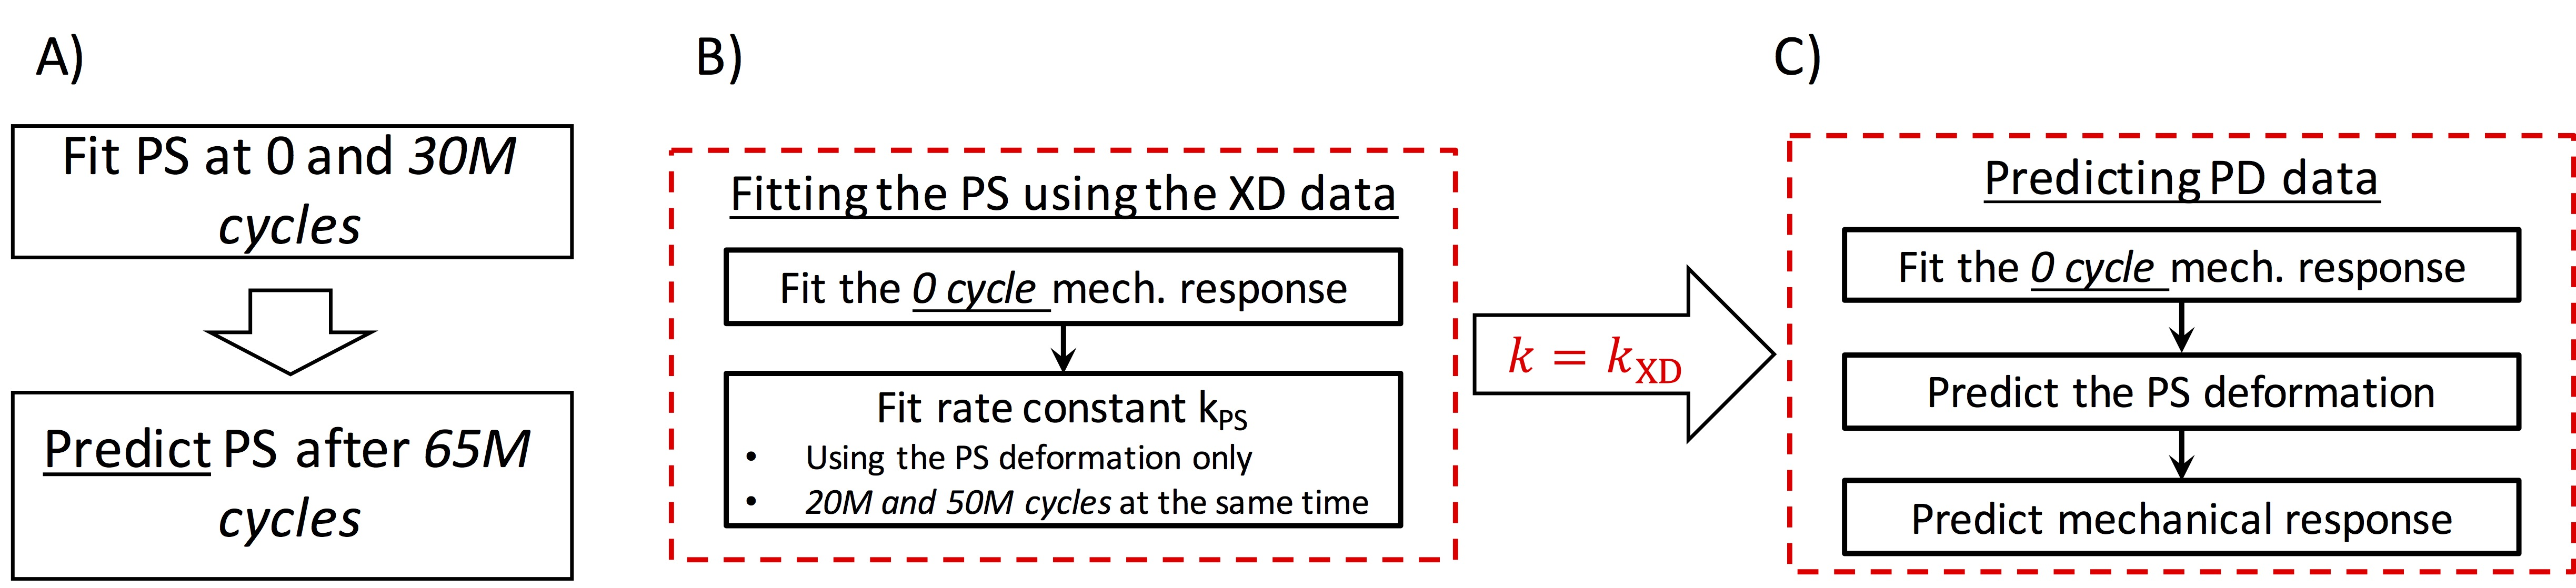
\includegraphics[width=\textwidth]{Images/chapter4/figure12}}
\caption{Our parameter estimation approach for the A) strain controlled cyclic loading data, B) stress controlled data cycled in the cross-preferred direction and C) in the preferred direction}
\label{fig:datamethods}
\end{figure}


%%%%%%%%%%%%%%%%%%%%%%%%%%%%%%%%%%%%%%%%%%%%%%%%%%%%%%%%%%%%
%%%%    Stress controlled cycling

\subsubsection{Stress controlled cycling}
The parameter estimation for the stress controlled specimens is more complicated than the strain controlled specimens as we do not know the strain history \textit{a priori}. This becomes a dynamic simulation, and we need to use optimization to determine the strain history (Eqn. \ref{eq:optimization}) at each time point. Thus, this data set is well suited to validate the full model using time dependent simulations. Since we have data for both PD-loading and XD-loading, we can fit the XD-loading data and used the resulting rate constant $k $ to predict the PD-loading data. First, we discretized the problem as followed
\begin{equation} 
\begin{aligned}
\phi_m \mathbf{S}_m =& \phi_m \left[\mathrm{Exp} \left[-k  \cdot n \cdot \Delta s \right] \mathbf{\bar{S}}_m \left(\mathbf{F}_\mathrm{PS}, \mathbf{I},\mathbf{C}\right)\vphantom{\sum_{i = 1}^n}\right. \\
&+ \left.\sum_{i = 1}^n  (k \Delta s) \mathrm{Exp}\left[-k (n\Delta s - i \Delta s)\right] \mathbf{\bar{S}}_m \left(\mathbf{F}_\mathrm{PS}, \mathbf{A}(i\Delta s),\mathbf{C}\right)\right].
\end{aligned}
\end{equation}
After each time step $\Delta s$, we compute the new loaded state $\mathbf{A}(i\Delta s)$ using optimization(Eqn. \ref{eq:optimization}, Fig. \ref{fig:implementation}). Through preliminary trials, the most optimal resolution in time is $\Delta s = 1$ million cycles when considering both time to run the simulations and accuracy of the results. We note that since an additional optimization is added to the parameter estimation process, we can no longer fit both the permanent set deformation $\mathbf{F}_\mathrm{PS}$ and the mechanical data at the same time. Our attempts at fitting both at the same time were not able to converge. Thus, we choose to predict the mechanical data as a way to validate our results. 
The parameter estimation process for the XD-loading data is
\begin{enumerate}
\item Determine the 0-cycled mechanical response
\item Fit the permanent set deformation $\mathbf{F}_\mathrm{PS}$ 
	\begin{enumerate}
	\item choose a $k $
	\item choose a mounting direction $\theta_\mathrm{mount}^{20}$ for cycling up to 20 million cycles 
	\item compute $err_\mathrm{PS} = \mathbf{F}_\mathrm{PS} - \mathbf{F}_\mathrm{PS}^\mathrm{data}$ error at 20 million cycles
	\item choose a mounting direction $\theta_\mathrm{mount}^{50}$ for cycling from 20 to 50 million cycles 
	\item compute $err_\mathrm{PS} = \mathbf{F}_\mathrm{PS} - \mathbf{F}_\mathrm{PS}^\mathrm{data}$ error at 50 million cycles
	\item update $k$, $\theta_\mathrm{mount}^{20}$, and $\theta_\mathrm{mount}^{50}$ using Quasi-Newton
	\end{enumerate}
\item Predict the mechanical response 
\end{enumerate}
Next we, used $k $ from the XD-loading data to predict the PD-loading data. 
\begin{enumerate}
\item Determine the 0-cycled mechanical response
\item Compute Fit the permanent set deformation $\mathbf{F}_\mathrm{PS}$
	\begin{enumerate}
	\item set $k $ from XD-loading data
	\item choose a mounting direction $\theta_\mathrm{mount}^{20}$ for cycling up to 20 million cycles 
	\item compute $err_\mathrm{PS} = \mathbf{F}_\mathrm{PS} - \mathbf{F}_\mathrm{PS}^\mathrm{data}$ error at 20 million cycles
	\item choose a mounting direction $\theta_\mathrm{mount}^{50}$ for cycling from 20 to 50 million cycles 
	\item compute $err_\mathrm{PS} = \mathbf{F}_\mathrm{PS} - \mathbf{F}_\mathrm{PS}^\mathrm{data}$ error at 50 million cycles
	\item update $\theta_\mathrm{mount}^{20}$ and $\theta_\mathrm{mount}^{50}$ using Quasi-Newton
	\end{enumerate}
\item Predict the mechanical response 
\end{enumerate}

%%%%%%%%%%%%%%%%%%%%%%%%%%%%%%%%%%%%%%%%%%%%%%%%%%%%%%%%%%%%%%%%%%%%%%%%%%%%%%%%
%%%%    Parametric studies


\begin{figure}[hbt]
\centering
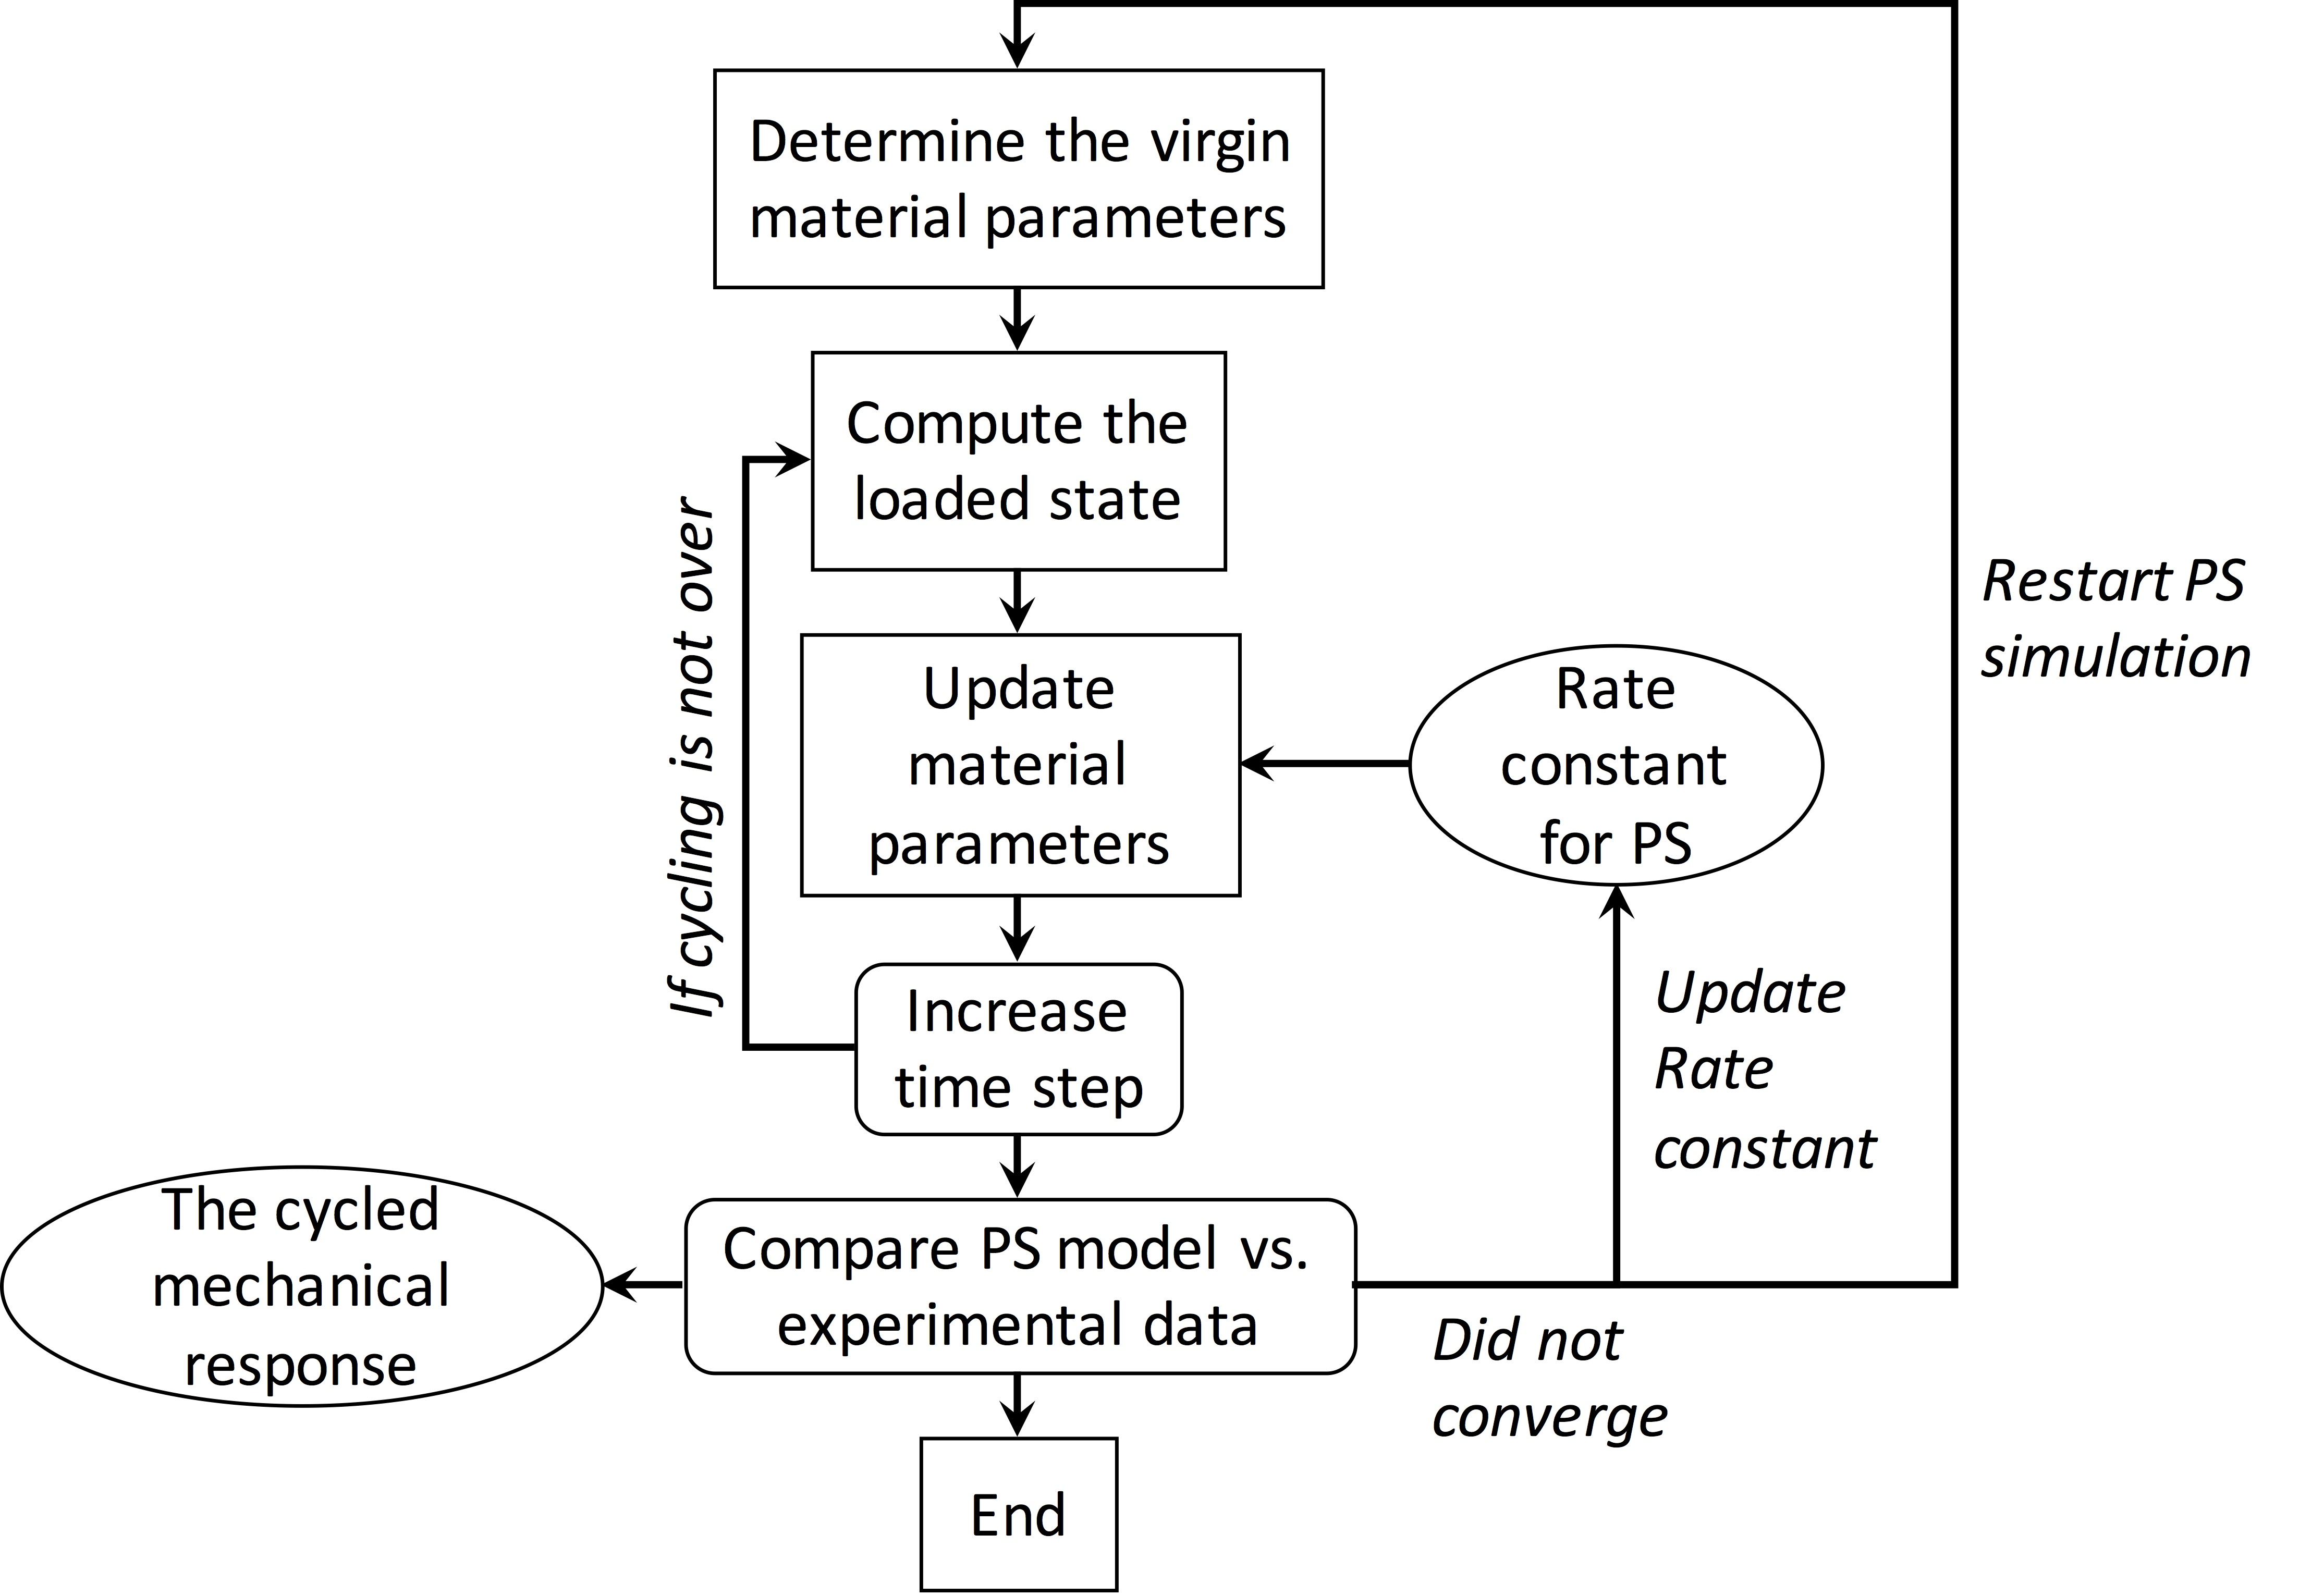
\includegraphics[width=5in]{Images/chapter4/figure13}
\caption{Implementation of the full model with updates in time.}
\label{fig:implementation}
\end{figure}


\subsection{Parametric studies}
Next, we performed an parametric study using the stress-controlled PD data. The same material parameters and rate constant, $k$, from parameter estimation results above was used. We simulated one specimen by extending the cycle duration to 100 million cycles to examine how the changes in geometry due to permanent set respond to an extended cycling period. 

%---    primary results
\section{Permanent set model results}
\subsection{Model fit and predictive capabilities}


	For the strain control specimens, we found that we were able to fit the permanent set deformations very well ($R^2 = 0.96$) (Fig. \ref{fig:strainresults}A). We were able to predict the mechanical response of the strain controlled specimens at 65 million cycles ($R^2 = 0.83$) (Fig. \ref{fig:strainresults}B\&C). 
	For the stress controlled specimens, we found we were able to fit the permanent set deformations for the XD specimens ($R^2 = 0.93$)(Fig. \ref{fig:stressXDdef}B), as well as predict the PD specimens very well ($R^2 = 0.97$) (Fig. \ref{fig:stressXDdef}C). 
	The resulting rate constant from both data sets shown no statistical difference ($p > 0.98$)(Fig. \ref{fig:stressXDdef}A). 
The mechanical response for the stress controlled XD specimens did not match as well in terms of the $R^2$ value($R^2 = 0.72$). 
	However, given none of the mechanical data was involved in the parameter estimate this was nevertheless a very good prediction. 
	For example, when comparing the model to the experimental data by extrapolating the loading path of the equibiaxial protocol and finding the peak strain at 1MPa, the $R^2$ value increases to 0.93. 
	One the other hand, the predicted mechanical response for the PD controlled data were very good ($R^2 = 0.95$) (Fig. \ref{fig:stressPDmech}), suggesting that our model was able to capture the underlying mechanisms. 
	These results agree with our hypothesis that the initial changes in the mechanical response (in the first 50 million cycles) can be predicted by the change in microstructure alone, and that structural damage is low at this stage. 
\begin{figure}[hbt]
\centering
\centerline{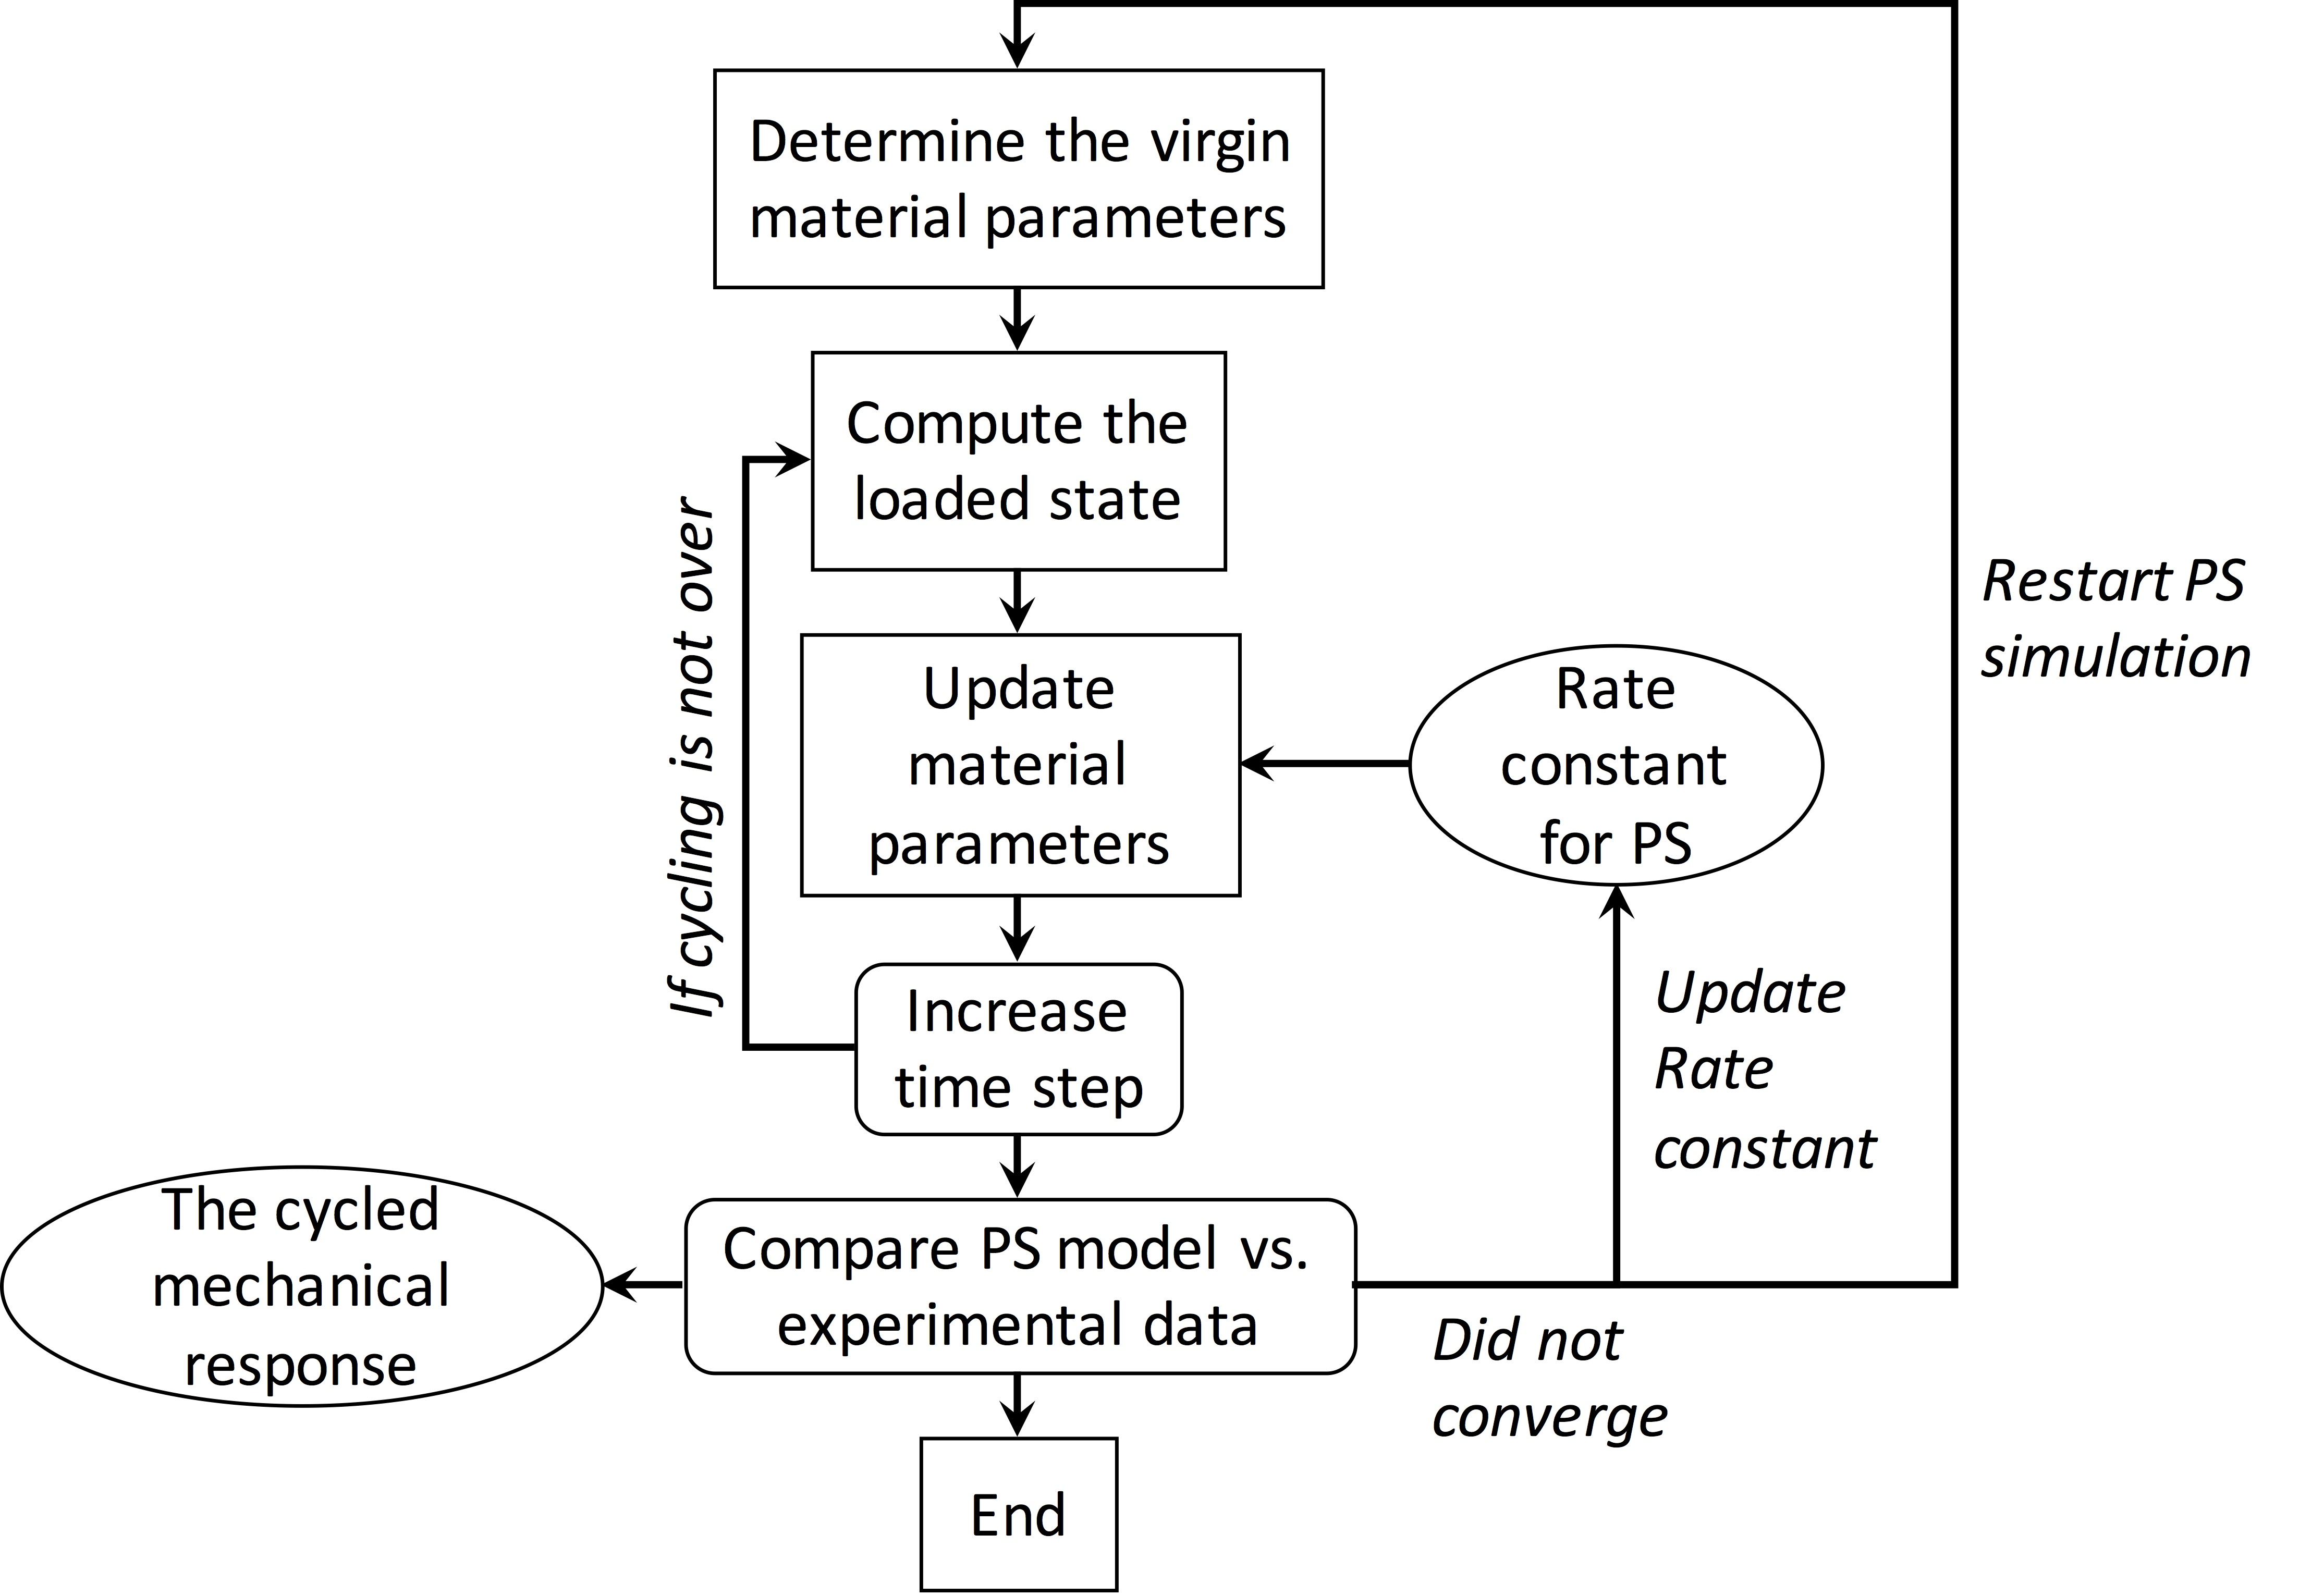
\includegraphics[width=0.75\paperwidth]{Images/chapter4/figure13}}
\caption{Results of the strain controlled cycling data, shown how the A) model fits the permanent set deformation at 30 million cycles and predicts the 65 million cycles time point(in box), as well as C) how the model predicts the mechanical response at 65 million cycles using material parameters from the B) 0 cycle time point.}
\label{fig:strainresults}
\end{figure}
\begin{figure}[hbt]
\centering
\centerline{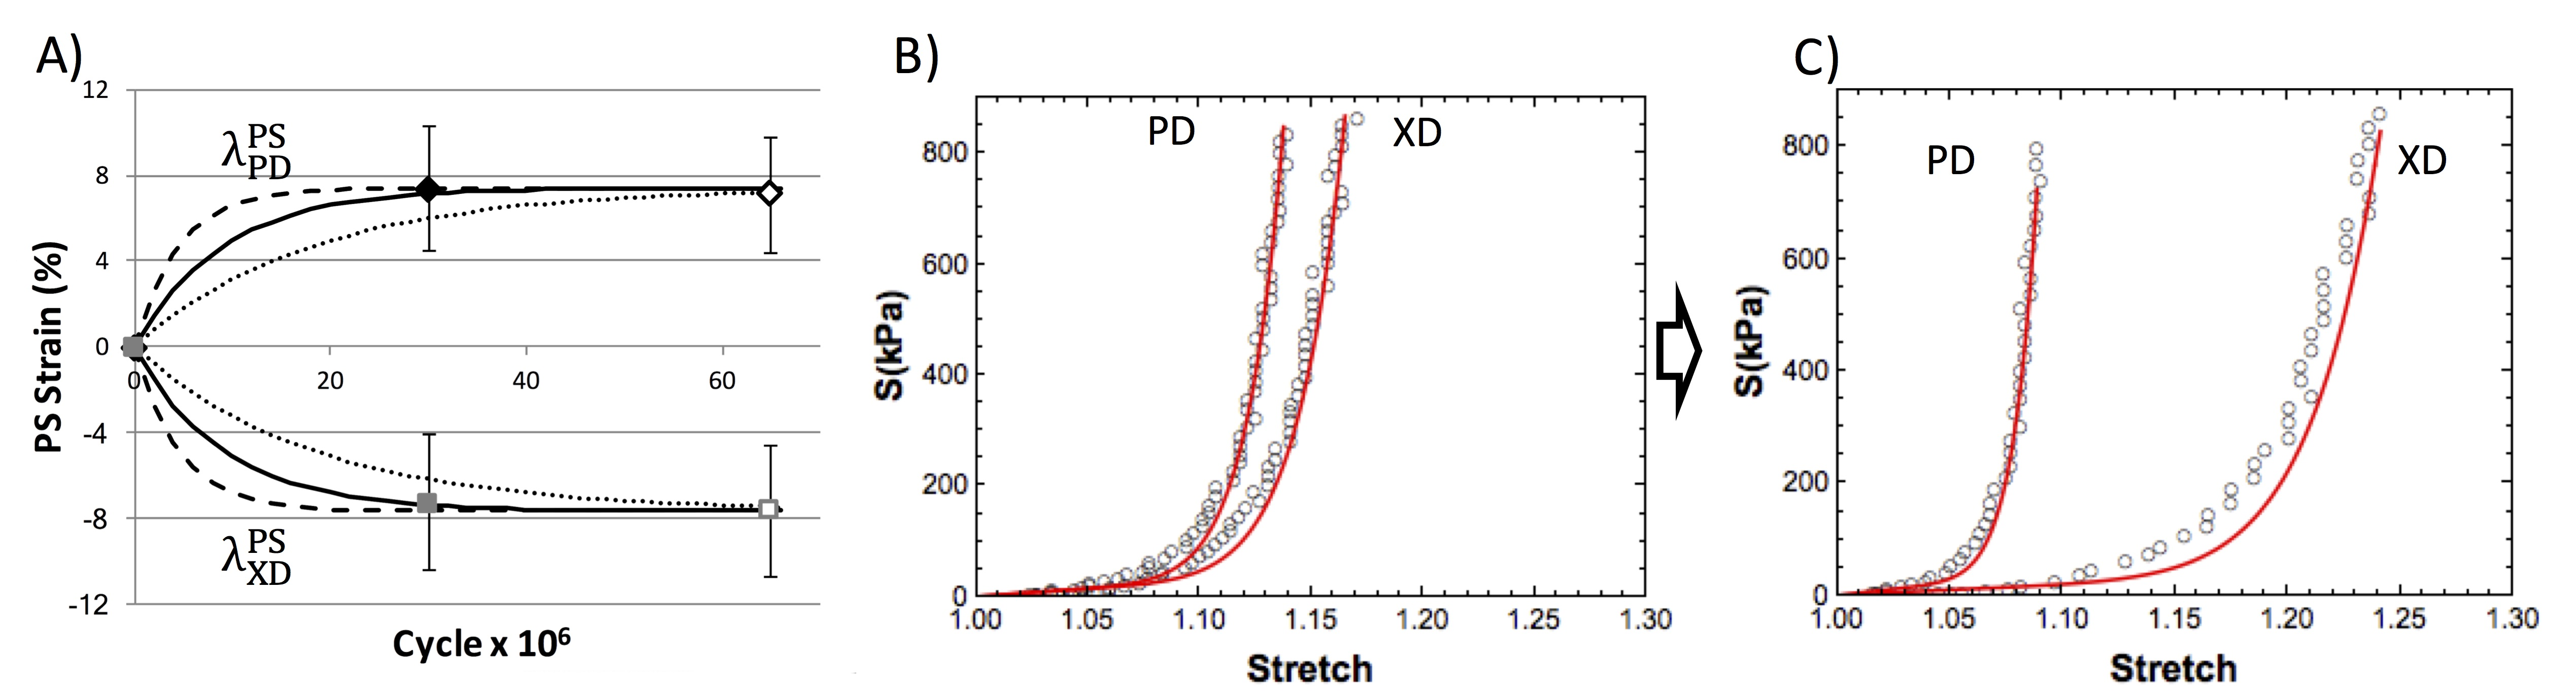
\includegraphics[width=0.75\paperwidth]{Images/chapter4/figure14}}
\caption{A) The model fit for the permanent set deformation at both 20 and 50 million cycles for the stress controlled XD cycled specimens. B) Comparison of the permanent set rate constant between the strain controlled and stress controlled specimens. C) The predicted permanent set deformation for the PD cycled specimens using the rate constant from fitting the XD cycled specimens. }
\label{fig:stressXDdef}
\end{figure}
\begin{figure}[hbt]
\centering
\centerline{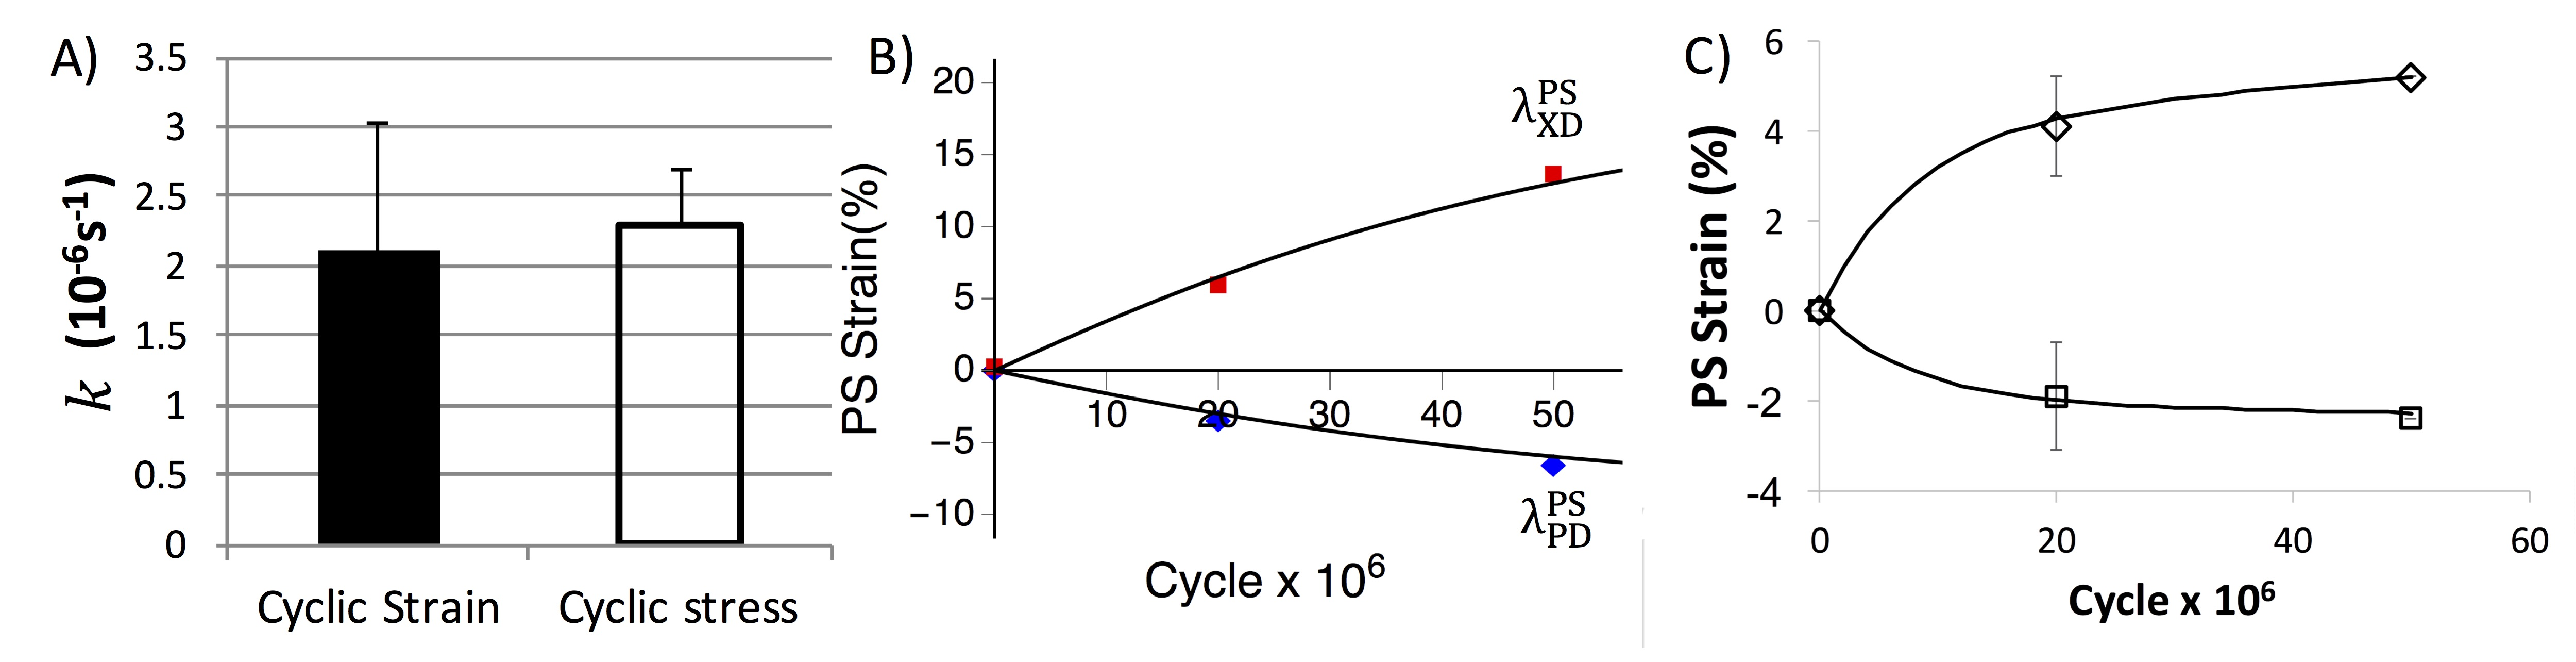
\includegraphics[width=0.75\paperwidth]{Images/chapter4/figure15}}
\caption{A) Best fit of the mechanical response at 0 cycle for the material parameters ($r^2 = 0.98$). The predicted mechanical response for the representative PD cycled specimen at B) 20 ($r^2 = 0.87$) and C) 50 million cycles. ($r^2 = 0.82$)}
\label{fig:stressPDmech}
\end{figure}

\subsection{Parametric study results}
	By extending the cycling duration in the parametric study, we found that the permanent set deformation reaches an assymptote after approximately 70 million cycles when loading along the PD. 
	This threshold slightly exceeds the lower bound for collagen recruitment. 
	We estimate that around 2.6\% of collagen fiber are recruited when the permanent set deformation reaches this threshold (Fig. \ref{fig:parametric}). 
	This suggests that collagen fibers are limiting the maximum change in geometry that can occur, and that the lower bound of the collagen fiber recruitment can serve as an estimated bound for the change in geometry due to the permanent set effect in BHVs, as collagen fibers start resisting further deformation of the exogenously crosslinked the matrix. Once this bound is exceed, some collagen fibers can exist perennially in an extended state. This could be a potential mechanism in exacerbating the rate of damage to the collagen fiber architecture. 

\begin{figure}[hbt]
\centering
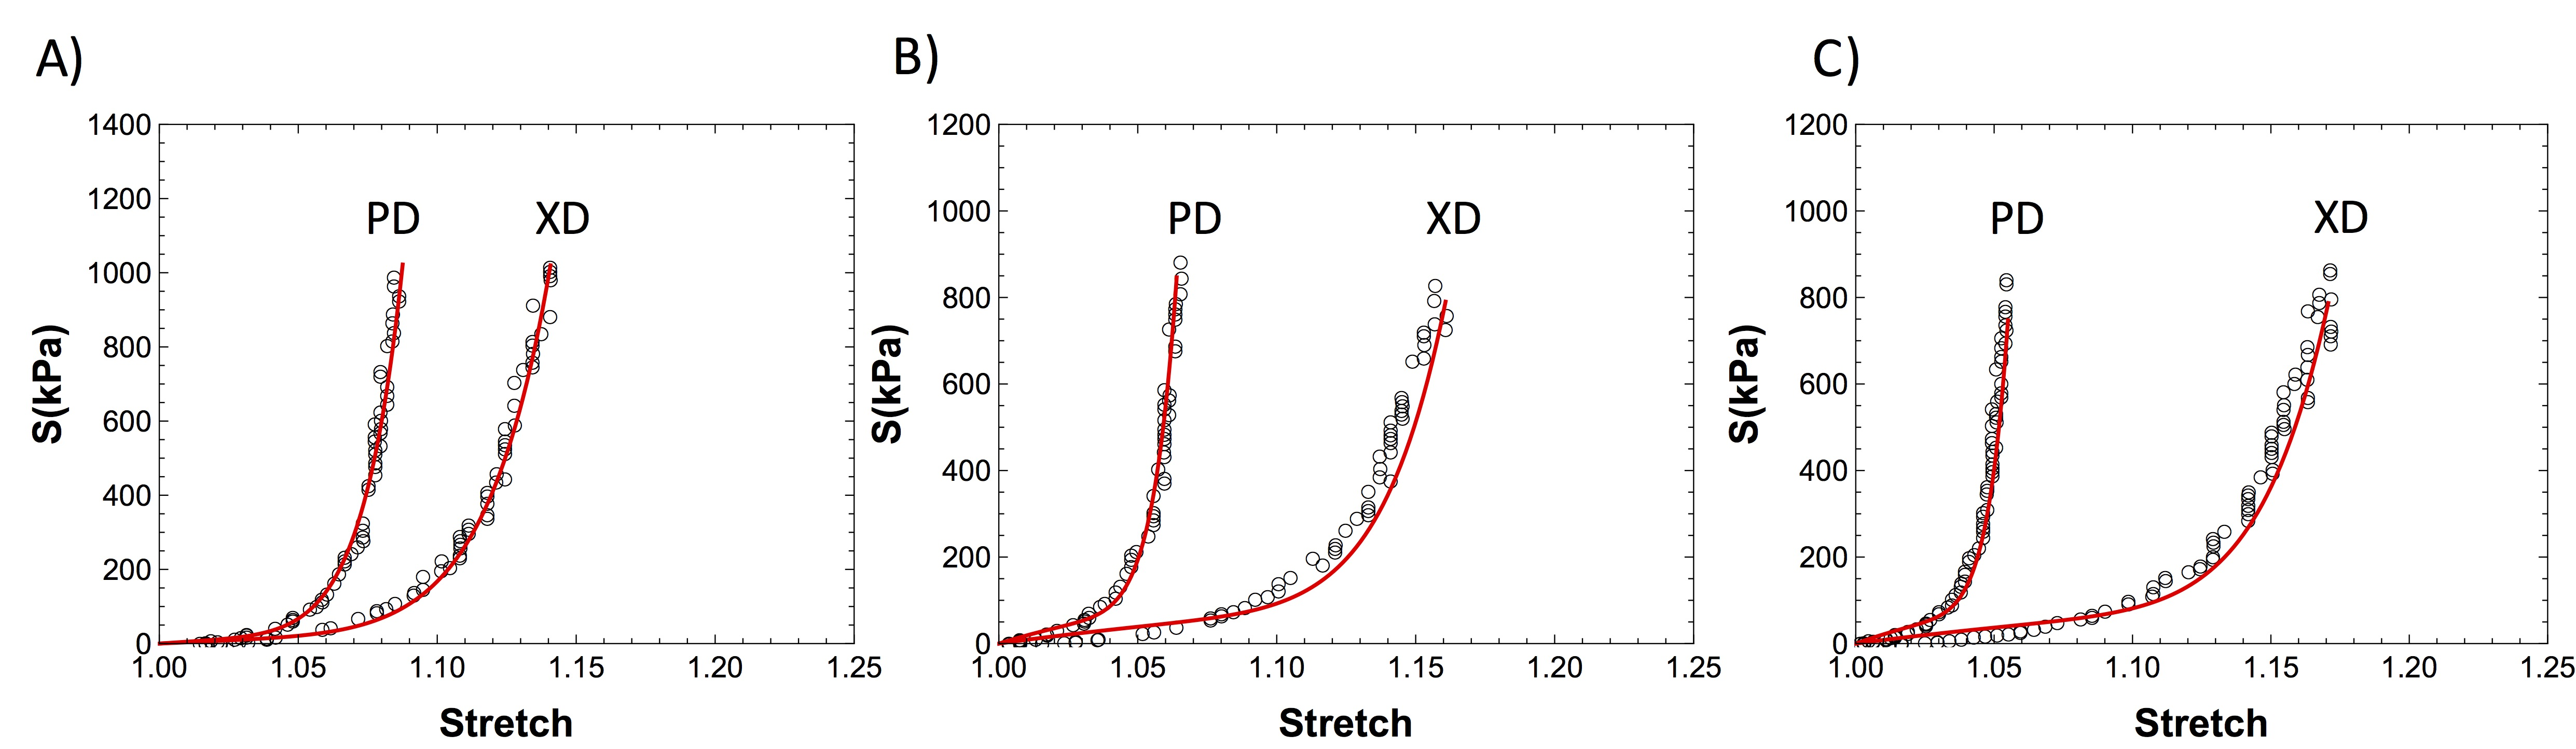
\includegraphics[width=0.35\paperwidth]{Images/chapter4/figure16}
\caption{The results of the parametric study. The red solid line shows the lower bound for the collagen fiber slack stretches and the red dashed line show the approximate cycle when the permanent set stretches reach an assymptote.}
\label{fig:parametric}
\end{figure}

%---    discussion
\section{Discussion}

\subsection{Permanent set is sufficient to describe early stages of BHV cycling}
	The most important result from this study is that permanent set alone is sufficient to explain all responses due to cyclic loading in the range of 0 to 65 million cycles. 
	This strongly suggests that there is no detectable damage to the collagen fiber architecture, and that the overall collagen fiber architecture stays intact and convected under affine kinematics. 
	This is not unexpected, as we previously found dense collagenous tissues to behave affinely when deforming in the physiological range \cite{lee_presence_2015}. 
	Although the permanent set effect is very noticeable in the early stages of the cyclic loading, it still takes millions of cycles; in other words, years. 
	Due to the time scale difference between the opening and closing of heart valves versus permanent set, BHVs always deforms quasi-statically, which means it always follows affine kinematics. 
	It follows that any structural changes in the collagen fiber architecture is affine as well. 
	This is all extremely important, as this allows us to completely separate permanent set from other cyclic loading effects and independently determine the permanent set rate constant just from the cyclic loading data in the early stage. 

\subsection{Lack of detectable structural damage}
	We observed in multiple instances \cite{sun_response_2004, sellaro_effects_2007} that there are molecular conformation changes in the collagen fiber during this early stage. 
	This suggests that while effects of collagen fiber damage are not detectable, it remains an ongoing but much slower process in comparison to permanent set. 
	Significant tearing and delamination are observed by Sacks and Smith \cite{sacks_effects_1998} after 500 million cycles, but this corresponds to the late stage of cyclic loading (Fig. \ref{fig:hypothesis}) during which we do not have extant mechanical data for constitutive modeling. 
	There are no other existing experimental data quantifying the intrinsic structural damage in BHVs during cyclic loading. 
	This is not surprising as actual structural damage is difficult to distinguish from other processes such as permanent set. 
	The relation between molecular changes and mechanical response is not well understood. 
	This requires multi-scale modeling for exogenously crosslinked tissue, which is also an extremely challenging task with no published studies currently. 
	The most promising way of quantifying structural damage is through constitutive modeling and simulations. 
	Structural models can separate structural damage and permanent set, but we do not have sufficiently data at high cycle numbers where structural damage is detectable. 
	This remains an important extension for the model in the future. 

\subsection{Permanent set is driven by the scission-healing of the matrix}
	One important assumption in our model is that permanent set only occurs in the matrix due to scission-healing. 
	Based on our theory for permanent set, the process is driven entirely by the first order kinetics of the crosslinking reactions of GLUT leading to scission-healing, as well as the kinematics involved in the reference state evolution. 
	Our results indicate that these mechanisms and permanent set can indeed explain the response to cyclic loading.
	This highlights the importance of understanding the effects of GLUT crosslinks and its role in the cyclic loading response of BHVs. 
	The use of GLUT was originally intended for suppressing immunogenicity by crosslinking antigen within BP xenographs, but also has the fortunate consequence of stiffening the mechanical response of the BHV. 
	Unfortunately, the scission-healing behavior of GLUT also playing a major role in the cyclic loading of BHVs. 
	By severely changing the geometry of the BHV in the first 1-2 years, it strongly influences the cyclic loading response of BHVs at latter stages. 
	It is difficult to properly design BHVs without accounting for the permanent set deformations caused by GLUT's scission-healing. 
	Alternative exogenous crosslinking chemistry \cite{tam_fixation_2017, tam_novel_2015} may be an important area for technological advancement of BHVs. 
	Protecting the optimal mechanical response of the BHVs by reducing the impact permanent set can significantly limit the peak stress on BHVs and protect the underlying tissue microstructure. 

\subsection{Recruitment of collagen fibers limit permanent set}
	Our parametric study of permanent set suggests that collagen fibers may play a significant role in limiting the effect of permanent set on the geometry of BHVs. 
	The stiffness of collagen fibers are over three magnitudes higher than the exogenously crosslinked matrix. 
	As collagen fibers are recruited, residual stress starts accumulating between collagen fibers and the matrix. 
	However, due to the significant difference in stiffness, the exogenously crosslinked matrix cannot extend the collagen fibers by a significant amount. 
	In addition, we generally found significant collagen fiber structural reserves in collagenous tissue \cite{zhang_meso_2016}. From the parametric study, no more than 2-4\% of collagen fibers are straightened under physiological loading levels (up to 1 MPa). 
	Also, taking into account the rapid recruitment of native collagen fibers (collagen fibers do not extend by more than 5-8\% strain before breaking \cite{buehler_atomistic_2006}), the collagen fiber architecture serves as a barrier in limiting the changes in geometry due to permanent set. 
	This potentially gives us a way of predicting and designing BHVs based on the expected maximum permanent set deformation. 

%---    discussion
%%%%%%%%%%%%%%%%%%%%%%%%%%%%%%%%%%%%%%%%%%%%%%%%%%%%%%%%%%%%%%%%%%%%%%%%%%%%%%%%
%%  Conclusions
%%%%%%%%%%%%%%%%%%%%%%%%%%%%%%%%%%%%%%%%%%%%%%%%%%%%%%%%%%%%%%%%%%%%%%%%%%%%%%%%


\section{Summary and Future Directions}
	We have developed the first structural-based constitutive model for the time evolving properties of exogenously crosslinked collagenous soft tissues under cyclic loading. We focused on permanent set as the mechanism for the geometry changes in the early stage of cycling and developed our constitutive model based on the underlying scission-healing reaction of the GLUT crosslinked matrix. Permanent set allows the reference configuration of the exogenously crosslinked matrix to evolve over time and convect the collagen fiber architecture through the change in geometry. The results show that permanent set alone is sufficient to explain all changes in the early stage of BHV cycling, and more importantly predict how the shape and reference configuration evolve during this stage. 	Moreover, structural damage does not play a detectable role up to 65 million cycles. Our model also indicates that the collagen fiber architecture can play a role in limiting the permanent set effect, where the straightening of collagen fibers prevents further changes in geometry. Thus, accounting for the permanent set effect is especially important in the design of BHVs to better improve their performance and durability. 
	
	In addition to the exogenously crosslinked tissue applications addressed herein, we have observed permanent set like phenomenon in mitral valve tissue during pregnancy \cite{rego_mitral_2016}. In that study, our results suggested that much of the growth and remodeling in the MV leaflet does not begin immediately, but rather undergoes mostly passive leaflet enlargement until these parameters reach a critically low level, at which point growth and remodeling are triggered. This initial tissue distension process is very similar in behavior to the permanent set mechanism outlined in the present work. Thus, the current approach could be applied to these types of the early phases soft tissue remodeling, where non-failure mechanisms occur before the onset of growth of tissue growth and remodeling. In addition, although the permanent set model we described only include the remodeling of the matrix due to scission-healing, the same concept can be extended by separating the rate constant into growth and resorption to simulate growth and remodeling of the matrix. Furthermore, the frame work outlined in section 5 can also be extended for the remodeling of the collagen fiber architecture, given further studies on mechanisms for how the collagen fiber architecture grows once the critical level observed in Rego \textit{et al} \cite{rego_mitral_2016} is exceeded. This is the advantage for the structural-based approach to modeling permanent set, which allows us to describe the mechanical response based on real physically measure-able quantities. We can further extend the more toward effects such as structural damage are the fiber-level, proteolytic degradation, and growth based on how this effects affect the components of the permanent set model layed out herein.

\newpage
%%%%%%%%%%%%%%%%%%%%%%%%%%%%%%%%%%%%%%%%%%%%%%%%%%%%%%%%%%%%%
%%  nomenclature											%
%%%%%%%%%%%%%%%%%%%%%%%%%%%%%%%%%%%%%%%%%%%%%%%%%%%%%%%%%%%%%
\section*{Nomenclature} \label{c4:sec:nomenclature}
\begin{mynom}
\textbf{Key Terms}   \\
{Matrix}\>\>\tabfill{Non-fibrous part of the extracellular matrix }  \\
{EXL}\>\tabfill{Exogenously crosslinked}  \\
{PS}\>\tabfill{Permanent set, an irreversible deformation that remains in a structure or material after it has been subjected to stress.}  \\
{Damage}\>\>\tabfill{Loss of mechanical properties}  \\
{Fatigue}\>\>\tabfill{Weakening of a material caused by repeated loading}  \\
{Plastic deformation}\>\>\>\>\>\tabfill{Deformation of a material undergoing irreversible change in shape in response to applied forces}  \\
{Structural convection}\>\>\>\>\>\>\tabfill{A permanent deformation of the collagen fiber architecture based on the change in the reference configuration}  \\
{BP}\>\tabfill{Bovine pericardium}  \\
{CFA}\>\tabfill{Collagen fiber architecture}  \\
{BHV}\>\tabfill{Bioprosthetic heart valve}  \\
{AWT}\>\tabfill{Accelerated wear testing}  \\
{GLUT}\>\tabfill{Glutaraldehyde}  \\
{TVI}\>\tabfill{Transcatheter aortic intervention }  \\
{PD}\>\tabfill{Preferred direction}  \\
{XD}\>\tabfill{Cross-preferred direction}  \\
{ODF}\>\tabfill{Orientation distribution function}  \\
{Recruitment}\>\>\>\tabfill{Probability distribution function describing the strain at which a collagen fiber's crimp is straightened }  \\ 
{Fiber ensemble}\>\>\>\>\tabfill{A group of fibers which share a common orientation}  \\
\textbf{Symbols}      \\
{$\Psi$}\>\tabfill{Strain energy}  \\
{$\Psi_\mathrm{col}, \Psi_\mathrm{int}, \Psi_m$}\>\>\>\tabfill{Strain energy of the collagen fiber, ensemble-ensemble interactons, and matrix components respectively}  \\
{$D$}\>\tabfill{Collagen fiber recruitment distribution function}  \\
{$\lambda_s$}\>\tabfill{The slack stretch, the stretch needed to straighten the collagen fiber crimp }  \\
{$\Gamma$}\>\tabfill{Collagen fiber orientation distribution function}  \\
{$\phi$}\>\tabfill{Mass fraction}  \\
{$\eta_C$, $\eta_m$, $\eta_I$}\>\>\>\tabfill{The modulus of collagen, EXL matrix and fiber-fiber interactions}  \\
{$\mathbf{I}$}\>\tabfill{Identity tensor}  \\
{$\mathbf{F}$}\>\tabfill{An arbitrary deformation gradient tensor applied to the tissue, referenced to the original uncycled stress free state}  \\
{$\mathbf{C}$}\>\tabfill{Right Cauchy-Green strain tensor, referenced to the original uncycled stress free state}  \\
{$\mathbf{E}$}\>\tabfill{Green Lagrange strain, referenced to the original uncycled stress free state}  \\
{$\lambda$}\>\tabfill{Stretch}  \\
{$\mathbf{n}_\alpha$}\>\tabfill{A vector pointing at the angle $\alpha$ }  \\
{$\lambda_\alpha = \sqrt{\mathbf{n}_\alpha \cdot \mathbf{C} \mathbf{n}_\alpha}$}\>\>\>\>\tabfill{The applied stretch at the fiber ensemble-level in the direction $\alpha$ }  \\
{$\prescript{}{\alpha}{\lambda}_s$}\>\tabfill{The slack stretch of a collagen fiber oriented with the angle $\alpha$ }  \\
{$\mathbf{S}$}\>\tabfill{Second Piola Kirchhoff tensor, referenced to the original uncycled stress free state}  \\
{$I_1$}\>\tabfill{First invariant}  \\
{$I_8$}\>\tabfill{Eighth pseudo invariant}  \\
{$I_8^rot$}\>\tabfill{The rotational component of $I_8$ }  \\
{$I_8^ext$}\>\tabfill{The extensional component of $I_8$ }  \\
{$k$}\>\tabfill{Rate constant for permanent set}  \\
{$s$}\>\tabfill{The current time in seconds }  \\
{$\hat{s}$}\>\tabfill{The intermediate time when the EXL matrix is formed by the scission-healing process }  \\
{$\Omega_0$}\>\tabfill{The original unloaded configuration of the tissue before any cyclic loading}  \\
{$\Omega(s)$}\>\tabfill{The current loaded configuration of the tissue during cyclic loading}  \\
{$\mathbf{A}(s)$}\>\tabfill{Strain history, which is the root mean square strain of each cycle as a function of time}  \\
{$\mathbf{\tilde{B}}(s) = \mathbf{A}\mathbf{A}^\mathsf{T}$}\>\>\>\tabfill{Left Cauchy Green tensor of the strain history}  \\
{$\mathbf{\bar{F}}(\hat{s})$}\>\tabfill{Deformation gradient tensor applied to the tissue, referenced to the strain history $\mathbf{A}(\hat{s})$ at time $\hat{s}$}  \\
{$\mathbf{\bar{C}}(\hat{s})$}\>\tabfill{The right Cauchy Green strain tensor applied to the tissue, referenced to the strain history $\mathbf{A}(\hat{s})$ at time $\hat{s}$}  \\
{$\bar{I}_1$}\>\tabfill{Modified first invariant, referenced to the strain history $\mathbf{A}(\hat{s})$ at time $\hat{s}$}  \\
{$\bar{\mathbf{\Psi}}_m$}\>\tabfill{Strain energy of the matrix as function of $\bar{I}_1$}  \\
{$\bar{\mathbf{S}}_m$}\>\tabfill{Stress of the matrix as function of $\bar{I}_1$}  \\
{$\Omega_\mathrm{PS}(s)$}\>\tabfill{The current unloaded configuration due to changes in geometry caused by permanent set}  \\
{$\mathbf{F}_\mathrm{PS}(s)$}\>\tabfill{The deformation from $\Omega_0$ to the current unloaded configuration ($\Omega_\mathrm{PS}$) due to permanent set}  \\
{$b(s)$}\>\tabfill{The proportion of the existing amount of material remaining}  \\
{$a(s,\hat{s})$}\>\tabfill{The proportion of the material newly formed at time $\hat{s}$ remaining}  \\
{$\prescript{1}{0}{\mathbf{F}}$}\>\tabfill{The deformation gradient from $\Omega_0$ to some arbitrary state $\Omega_1$, most commonly $\Omega_1 = \Omega_\mathrm{PS}$ }  \\
{$\prescript{1}{0}{\lambda}(\theta_0)$}\>\tabfill{The stretch of an ensemble oriented along $\theta_0$ in $\Omega_0$ deformed from $\Omega_0$ to some arbitrary state $\Omega_1$}  \\
{$D_1$}\>\tabfill{The collagen fiber recruitment distribution function convected from $\Omega_0$ to to some arbitrary state $\Omega_1$ }  \\
{$\Gamma_1$}\>\tabfill{The collagen fiber orientation distribution function convected from $\Omega_0$ to to some arbitrary state $\Omega_1$}  \\
{$\mathbf{\hat{S}}$}\>\tabfill{The applied stress during cyclic loading }  \\
\end{mynom}

\newpage
%---    Bioliography
\bibliographystyle{plainnat}
\bibliography{phd}



\chapter{Homogenization and upscaling of structural and multi-scale models using effective constitutive models for facilitating numerical simulations}

\section*{Preface}
\addcontentsline{toc}{section}{Preface}%

One of the most crucial aspects of biomechanical simulations of organs and systems that seek to predict the outcomes of disease, injury, and surgical interventions is the underlying constitutive model. Current soft tissue constitutive modeling approaches have become increasingly complex, often utilizing meso- and multi-scale methods for greater predictive capability and linking to the underlying mechanisms. However, such modeling approaches are associated with substantial computational costs. One solution is to use effective constitutive models, which only reproduces the essential responses but not the underlying mechanisms. Effective constitutive models can be implemented in place of meso- and multi-scale models in numerical simulations, but derive their responses by homogenizing the responses of the underlying meso- or multi-scale models. A robust effective constitutive model can thus drastically increase the speed of simulations for a wide range of meso- and multi-scale models. However, there is no general consensus on how to develop a single effective constitutive model for a wide range of soft tissue responses. In the present study, we developed an effective constitutive model, which can fully reproduce the response of a wide range of planar soft tissue responses, along with methods for fast-convergent parameter estimation. We evaluated this approach and demonstrated that it is able to handle materials of widely varying degrees of anisotropy, such as exogenously cross-linked bovine pericardium and aortic valve leaflet. This effective constitutive model approach has shown significant potential for improving the computational efficiency and numerical robustness of multi-scale and meso-scale modeling approaches, facilitating the application of inverse modeling and simulations of growth and remodeling of soft tissues and organs.

\textbf{The work contained in this chapter was published as}: Zhang, W., Zakerzadeh, Z., Zhang, W. \& Sacks, M. S.
A Material Modeling Approach for the Effective Response of Planar Soft Tissues for Efficient Computational Simulations. 
Journal of the mechanical behavior of biomedical materials. under review.



%---    INTRODUCTION
%%%%%%%%%%%%%%%%%%%%%%%%%%%%%%%%%%%%%%%%%%%%%%%%%%%%%%%%%%%%%
%%  Introduction											%
%%%%%%%%%%%%%%%%%%%%%%%%%%%%%%%%%%%%%%%%%%%%%%%%%%%%%%%%%%%%%

\section{Introduction}

%-------	Computational approaches	-------%
	Computational studies of organs and bioprosthetic devices have become increasingly popular for predicting the outcomes of diseases, injuries, and surgical interventions. Such applications include the simulation of aneurysm growth \cite{rissland_abdominal_2009,ramault_comparison_2010,hoi_effects_2004,volokh_model_2008}, blood flow \cite{olufsen_numerical_2000,perktold_computer_1995,pries_blood_1990,oshima_finite_2001,bagchi_mesoscale_2007}, and natural or bioprosthetic heart valves \cite{zakerzadeh_computational_2017, soares_biomechanical_2016, kamensky_immersogeometric_2015, aggarwal_vivo_2016, nobili_numerical_2008, cheng_three_2004}. One of the most important components of predictive simulations is an accurate constitutive model that can predict the mechanical behavior of the soft tissues and biomaterials involved. Such tissues have highly nonlinear anisotropic behaviors, often resulting in specific forms for different tissue types. In addition, these constitutive models are often extended to model growth, remodeling, pathology, fatigue, trauma and other time evolving processes. As such, constitutive models are often developed to take advantage of the structure to function relationship to predict how the response of the materials will evolve, utilizing physical models, multi-scale approaches, and/or molecular dynamics. Not surprisingly, constitutive models are becoming exceeding complex, and the computational costs are becoming a hindrance to more complex numerical simulations. 


%-------    structural modeling    -------%
    Examples of such approaches are meso-scale structural approaches for soft tissue modeling \cite{lanir_constitutive_1983}. This class of soft tissue models homogenizes the tissue response at the meso-scale, where the simplified models of the mechanical response of collagen, elastin and other fibers are integrated with tissue microstructure \cite{kassab_structure_2016}. This type of constitutive model has been shown to be able to accurately represent the mechanical behaviors of many soft tissues including valvular tissues \cite{zhang_meso_2016, rego_mitral_2016}, pericardium \cite{zhang_modeling_2017}, myocardium \cite{avazmohammadi_novel_2016}, and elastomeric scaffolds \cite{d.amore_large_2016}. Recently, we have extended these models to include interaction terms \cite{zhang_modeling_2017, avazmohammadi_novel_2016}, which require multiple integrals to accurately compute the strain energy of fiber interactions. 




%-------    multi-scale modeling    -------%
    In a broader context, multi-scale approaches utilize fundamental mechanisms at the micro-scale to derive the response of materials at the macro-scale. Often, multi-scale modeling begins at the molecular level, where the molecular structure of the constituents and the physical laws governing their interactions are well known and well-studied in chemistry and physics. At this level, molecular dynamics can be used to determine the mechanical response of constituent proteins. This can be upscaled to quaternary protein structures using coarse grain methods. This response is then integrated with higher level structures of the tissue to determine the response at even larger scales. Homogenization is thus critical in multi-scale modeling to simplify the response of the downscale models to improve the efficiency of simulations at higher scales. This process is repeated until the macro- or tissue-level. Examples using this approach are the modeling of collagenous tissues by Buehler \textit{et al.} \cite{buehler_atomistic_2006, buehler_nanomechanics_2008} and intermediate filaments of cells by Qin \textit{et al.} \cite{qin_multi_2010}. 
    
    
    However, numerical simulations using these approaches are also quite costly. They can only be used for simulating the response of the materials, but cannot be easily incorporated into inverse modeling and time-dependent frameworks. Even the computational cost of meso-scale structural approaches is five magnitudes higher than conventional phenomenological approaches. For more detailed cell or molecular level information, which is important for better understanding cellular environments and growth and remodeling, the exceedingly high computational cost of multi-scale approaches makes it difficult for them to be directly implemented in computational simulations. As such, the multi-scale models used in simulations need to be simplified.

%-------    modeling material behavior    -------%
    It is for this reason that many types of phenomenological models with computationally efficient forms, such as the generalized Fung type \cite{fung_biomechanics_1993}, Holzapfel-Gasser-Ogden \cite{holzapfel_new_2000}, generalized Ogden \cite{ogden_large_1972}, generalized Rivlin \cite{rivlin_large_1951}, and Humphrey models \cite{may-newman_constitutive_1998}, are popular for numerical simulations. These models utilize constitutive modeling approaches which do not take into account the underlying mechanisms, thus can only reproduce the mechanical response in the limited range of the experimental data utilized for parameter estimation. Furthermore, the mechanical data used and parameter estimation are not done in an optimal manner. This makes finding the optimal parameters inconsistent due to the high covariance between parameters. This is demonstrated in Sun and Sacks \cite{sun_biaxial_2003} for modeling pericardium under high in-plane shear. Here, it was shown that fitting only a subset of the loading paths acquired from biaxial mechanical testing cannot predict the remaining unfitted loading paths. Yet for \textit{in vivo} simulations, these constitutive models are often derived from incomplete data while being asked to predict the mechanical response under non-physiological and often unpredictable ranges of deformations. As the parameters of such models have no physical meaning, it is often difficult to extend them for time-dependent processes such as growth and remodeling or to average and produce a population representative. As such, accurate simulations often still require detailed mechanism-based models. 
    

%-------    effective model    -------%
    %-------    effective model    -------%
    To address these problems, an approach which can take advantage of mechanisms and predictive capabilities of micro-models (meso-scale, multi-scale, or other complex constitutive models) and the numerical efficiency of phenomenological approaches for simulations at the macro-scale is very beneficial. An effective constitutive model, based on phenomenological approaches, can be used to accurately reproduce the responses of a wide range of tissues using the same form, acting as an intermediate step between micro-models for material behavior and organ-level numerical simulations (Fig. \ref{fig:simulationframework}A). For each iteration of the simulation, whether forward, inverse, or time-evolving, the effective constitutive model is first fit to the micro-model(s) to determine the model parameters, then it is used to perform the actual numerical simulation. Subsequent updates to the evolving material properties, geometry, and boundary conditions are then performed (Fig. \ref{fig:simulationframework}B). This makes the effective constitutive models especially useful for the final upscaling step of multi-scale models, increasing their efficiency. However, developing a generalized effective constitutive model is not straightforward. In addition to the issues described above, no specific constitutive model has yet been developed that is able to capture the material response of a wide range of soft tissue responses. Typically, a different constitutive model is used for each soft tissue type. These issues remain to be reconciled if effective constitutive models are to be used to fully reproduce the response of micro-models in computational simulations. 
    
    
    Thus, we hereby develop an effective constitutive model for planar soft tissues and a parameter estimation approach for rapidly determining the model parameters from the micro-model. Planar constitutive models are a good starting point, which are applicable to a wide range of soft tissues such as arteries, skin, heart valve, cells, vocal folds, bladder wall, synovial membrane, cornea, and cranial membrane. For the form of the effective constitutive model, we require the following characteristics:
\begin{enumerate}
    \item Widely applicable in that it is able to faithfully reproduce a wide range of tissue responses
    \item Computationally efficient and numerically robust
    \item Allows for fast and accurate convergence during parameter estimation for upscaling micro-models, thus having the minimal number of and minimally covariant model parameters
    \item Easy to implement, no integrations or functions without closed-form expressions
\end{enumerate}
    Using meso-scale structural models as an example, we will examine the ability of the effective constitutive model to fit the mechanical response of micro-models for a wide range of deformations, examine the speed and convergence of parameter estimation, and demonstrate the use of the effective constitutive model to facilitate the simulation of heart valves with a wide range of material properties.
    
%%%%%%%%%%%%%%%%%%%%%%%%%%%%%%%%%%%%%%%%%%%%%%%%%%%%%%%%%%%%
%-------------------    begin FIGURE     -------------------%
\begin{figure}
\centering
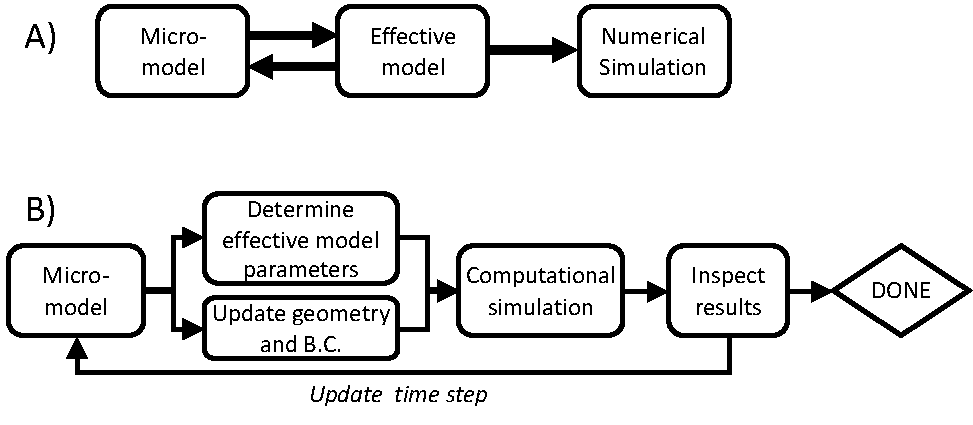
\includegraphics[width=\textwidth]{Images/chapter5/simulationframework}
\caption{Proposed framework for using an effective constitutive model to improve the efficiency of using complex meso- or multi-scale models (micro\Hyphdash models) in numerical simulations. Here, A) effective constitutive models act as an intermediate step between micro-models and numerical simulations, where micro-models inform the changes to the effective constitutive model while the effective constitutive model for the simulation. B) An example of how this may be implemented for time\Hyphdash evolving is shown.}
\label{fig:simulationframework}
\end{figure}
%-------------------     end FIGURE     -------------------%
%%%%%%%%%%%%%%%%%%%%%%%%%%%%%%%%%%%%%%%%%%%%%%%%%%%%%%%%%%%%
    
    
    
    
    
    
    
    


%---    METHODS
%%%%%%%%%%%%%%%%%%%%%%%%%%%%%%%%%%%%%%%%%%%%%%%%%%%%%%%%%%%%%
%%	Constitutive model form									%
%%%%%%%%%%%%%%%%%%%%%%%%%%%%%%%%%%%%%%%%%%%%%%%%%%%%%%%%%%%%%

\section{Effective constitutive model formulation}

%-----------------------------------------------------------
%	Kinematics
%-----------------------------------------------------------
\subsection{Kinematic considerations}
	
	The choice of kinematic basis is the first step to formulate constitutive models. Very often, it is useful to limit the choice of kinematic basis based on the available mechanical data or how well each basis match the response of the soft tissues, thus simplifying the form of the constitutive model and reducing parameter covariance during parameter estimation. However, for our approach, our aim is a highly generalized constitutive model that can match a wide range of possible micro-model responses using the same form, not restricting itself to the response and physics of specific soft tissue types. There is also no limitations to having sufficient mechanical data for parameter estimation, as this will be generated from the micro-models. As such, our considerations for choosing the kinematic basis are mainly:
\begin{enumerate}
    \item Most generalized form for reproducing a wide range of mechanical responses
    \item Simplest form for implementation and computational cost in numerical simulations
    \item Minimal number of parameters
    \item Minimal parameter covariance for parameter estimation
\end{enumerate}
    The smallest set of kinematic variables that can describe a wide range of soft tissues and deformations using the same simple form is ideal. 

    The invariants and pseudo-invariants of the right or left Cauchy Green tensor is very popular for the constitutive models of soft tissues. Indeed, we use them often with our structural models \cite{fata_insights_2014, zhang_meso_2016, Avazmohammadi2017b, sacks_novel_2016, zhang_modeling_2017}. There is a large number of invariants, each describes a facet of deformation: isotropic, volumetric strain, anisotropic, or interactions between them. The breadth of choices allow for more freedom in selecting a best combination when modeling specific soft tissues. However, there are simply too many invariants, and many of which are highly covariant. This does not lend itself for minimizing the number of parameters and the parameter covariance in a single fully generalized form. 
    
    
    It's here that using the components of the strain tensors is more practical for our approach. Although all strains are equivalent for constitutive modeling because they can be expressed with respect to each other, different strain tensors can have different effects when used directly in place of each other in the same form. For us, with the purpose of keeping the constitutive model form simple for implementation, the Green Lagrange strains are the most practical. Based on preliminary testing (Appendix \ref{sec:greenvshencky}), the Green Lagrange strains result in the simplest 2nd Piola Kirchhoff stress and elasticity tensor forms, and have behaviors in that closely matches the response of collagen fibers in soft tissues when under compression. We examined these aspects more closely in Appendix \ref{sec:greenvshencky}. 
    
    It is also convenient to express the Green Lagrange strain tensor with respect to the material axis (Fig. \ref{fig:greenkinematics}), $\mathbf{m}_0$, where
\begin{equation} \label{eqn:greenstrain}
E_m = \mathbf{m}_0\cdot\mathbf{E}\mathbf{m}_0, \quad E_n = \mathbf{n}_0\cdot\mathbf{E}\mathbf{n}_0, \quad E_{\phi} = \mathbf{m}_0\cdot\mathbf{E}\mathbf{n}_0,
\end{equation} 
    and $\mathbf{n}_0$ is the direction orthogonal to $\mathbf{m}_0$ (Fig. \ref{fig:greenkinematics}). This symmetry is helpful for further reducing the constitutive model form. 


%%%%%%%%%%%%%%%%%%%%%%%%%%%%%%%%%%%%%%%%%%%%%%%%%%%%%%%%%%%%
%-------------------	begin FIGURE 	-------------------%
\begin{figure}
\centering
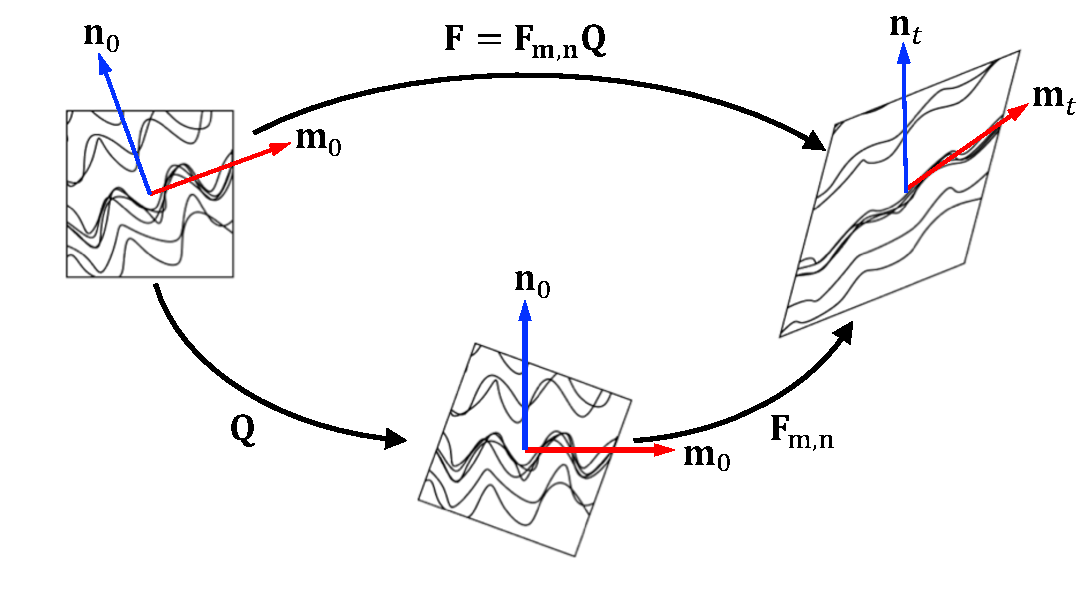
\includegraphics[width=5.0in]{Images/chapter5/greenkinematics.pdf}
\caption{By taking the right polar decomposition of the deformation gradient tensor, we can express the components of the Green Lagrange strain tensor with respect to the material axis. This creates a symmetry for the shear component of the Green Lagrange strain tensor, allowing us to further simplify the model form.}
\label{fig:greenkinematics}
\end{figure}
%-------------------	 end FIGURE 	-------------------%
%%%%%%%%%%%%%%%%%%%%%%%%%%%%%%%%%%%%%%%%%%%%%%%%%%%%%%%%%%%%












%-----------------------------------------------------------
%	Model formulation
%-----------------------------------------------------------
\subsection{Effective constitutive model form}
\subsubsection{Possible family of forms for the effective constitutive model}

    Using phenomenological approaches is necessary for minimal computational cost. The form of phenomenogical models for soft tissues generally falls into three families. The first family is composed of a summation of polynomials, 
%==========================================================%
%-------------------	begin EQUATION 	-------------------%
\begin{equation}
\begin{aligned}
\Psi	&= \sum_i\sum_j\sum_k c_{ijk}E_m^i E_n^j E_\phi^k. 
\end{aligned} \label{eqn:polynomialmodelform}
\end{equation}
%-------------------	 end EQUATION 	-------------------%
%==========================================================%
    We will refer to this family as the polynomial series approach. The second family is composed of separated exponential functions of individual or combinations of invariants or strains used, for example by Vito \textit{et al.} \cite{vito_mechanical_1980},
%==========================================================%
%-------------------	begin EQUATION 	-------------------%
\begin{align}\label{eqn:vitomodelforms}
\Psi 	&= \sum_i\sum_j\sum_k c_{ijk} e^{b_{ijk}E_m^i E_n^j E_\phi^k}.
\end{align}
%-------------------	 end EQUATION 	-------------------%
%==========================================================%
    We will refer to this family as the separated exponential approach. The final family is exponential models composed of a single exponential function of the sum of polynomials,
%==========================================================%
%-------------------	begin EQUATION 	-------------------%
\begin{equation}
\begin{aligned}\label{eqn:exponentialmodelform}
\Psi 	&= c_0 \left(e^{Q} - 1\right) \\
Q		&= \sum_i\sum_j\sum_k b_{ijk}E_m^i E_n^j E_\phi^k.
\end{aligned}
\end{equation}
%-------------------	 end EQUATION 	-------------------%
%==========================================================%
    This was first introduce by Fung \cite{fung_pseudoelasticity_1979} and we will refer to this family as the single exponential approach. 


\subsubsection{Generalized effective constitutive model form determination} \label{sec:possibleforms}

	Each approach (Eqn. \ref{eqn:polynomialmodelform}-\ref{eqn:exponentialmodelform}) has its own advantages and disadvantages. Polynomial series approach has the most flexibility. With sufficient number of terms, it can it reproduce the response in a similar manner to Taylor series expansions. In pilot testing, polynomial series approach requires significantly more number of terms than other choices, at least 27 terms in preliminary testing. 21 of the 27 terms are coupling terms. As a result, constraints needed for convexity are both complex and difficult to enforce. In the most general form, convexity cannot be enforce globally or only at the boundaries. It needs to be enforced at separate points within the domain or by integration. These constraints do not only have computational costs that vastly exceed the cost of the model itself, but will also significantly impacts convergence during parameter estimation. The constraints are not convex, with many local minima, often failing to converge even after 200,000 iterations. In additional, extrapolation using this approach is extremely unreliable. This makes constrained optimization often intractable to implement within a simulation framework such as the one proposed (Fig. \ref{fig:simulationframework}).


	The separated exponential approach generally suffers from the same issues as the polynomial series. This model form behaves like polynomial series with variable exponents, i.e. $c_1e^{b_1E_m} = c_1y^{b_1}$, where $y =e^{E_m}$. The advantage of this family of models is that similar and highly covariant terms such as $c_1 E_m + c_2 E_m^2 + c_3 E_m^3 ...$ can be avoided, reducing the number of parameters needed. However, like the polynomial series family, coupling terms such as $c_4 e^{b_4 E_m E_n}$ are not convex or elliptical functions, resulting in the same issues for parameter estimation and enforcing convexity. The number of parameters required to fully reproduce the mechanical response is still quite large. Moreover, for the same number of parameters, the separated exponential form is woefully insufficient at reproducing the mechanical response of soft tissues in comparison to the single exponential approach. As such, the advantages gained for parameter covariance by separating the terms are actually quite minimal.
    
    The single exponential approach has substantial parameter covariance, but is extremely effective at reproducing the response of soft tissues using a small number of parameters, is computationally efficient, and is easy to enforce convexity for. Because the exponential function is monotonically increasing, enforcing convexity and ellipticity only requires the polynomial $Q$ to be convex and elliptical. This is the best balance for our goals, and is thus our choice for the effective constitutive model. The first step is of course to examine the generalized Fung model \cite{fung_pseudoelasticity_1979}
%==========================================================%
%-------------------	begin EQUATION 	-------------------%
\begin{equation}
\begin{aligned}\label{eqn:fungmodel}
\Psi 	&= c_0 \left(e^{Q} - 1\right) \\
Q		&= \sum_i\sum_j\sum_k\sum_l b_{ijkl}E_{ij} E_{kl}.
\end{aligned}
\end{equation}
%-------------------	 end EQUATION 	-------------------%
%==========================================================%
    We find that the generalized Fung model is not able to fully reproduce the mechanical response of pericardium and aortic valve tissues, it can only do so in a limited range. Although this is enough for most numerical simulations, where the deformations are generally limited to the physiologic range, it is not always sufficient for predicting the mechanical response when organs undergo significant changes in geometry, causing the deformations to change drastically. The easiest way to visualize this is through contour plots of the strain energy function (Fig. \ref{fig:strainenergycontours}). The mechanical response of soft tissues general has hyperelliptical contours (Fig. \ref{fig:strainenergycontours}A), whereas the generalized Fung model always has precisely elliptical contours (Fig. \ref{fig:strainenergycontours}B). This attribute of the generalized Fung model makes it easy to enforce ellipticity and convexity, and its elasticity tensor and behavior at small strains is easy to derive. However, when the range of deformation is sufficiently large, the generalized Fung model is essentially limited to stretching and rotating its contours to match that of the soft tissue (Fig. \ref{fig:strainenergycontours}B), but cannot fully reproduce the resulting tissue responses. It can only serve as an approximation.  


%%%%%%%%%%%%%%%%%%%%%%%%%%%%%%%%%%%%%%%%%%%%%%%%%%%%%%%%%%%%
%-------------------	begin FIGURE 	-------------------%
\begin{figure}
\centering
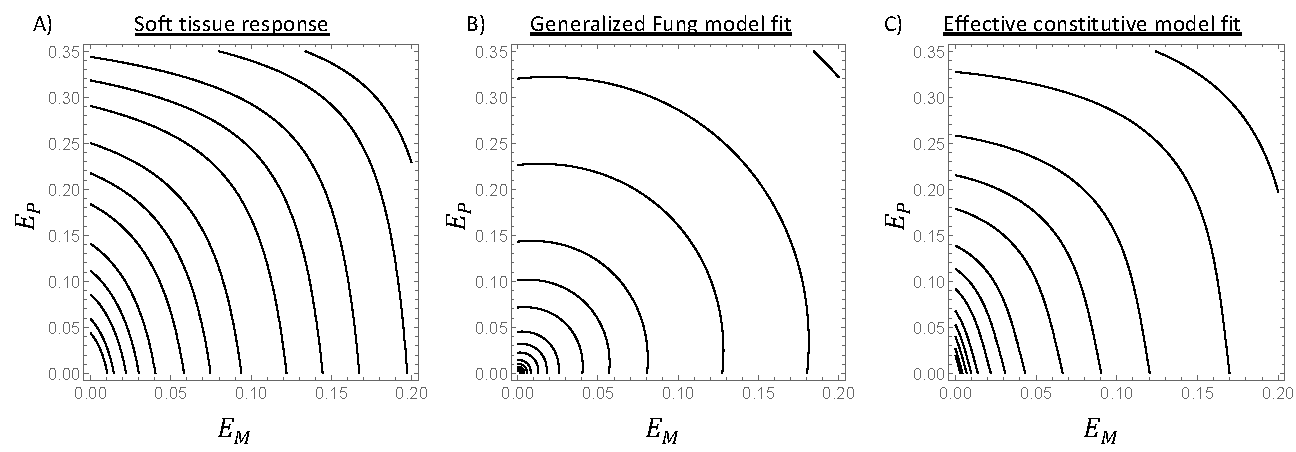
\includegraphics[width=\textwidth]{Images/chapter5/strainenergycontours}
\caption{The contour plots of strain energy (kPa) of A) a bovine pericardial specimen using a meso-scale structural model \cite{zhang_modeling_2017}, B) best fit using the generalized Fung model (Eqn. \ref{eqn:generalizedfungmodel}), and C) best fit using the effective constitutive model we develop from herein showing the necessity of extending existence phenomenological model form.}
\label{fig:strainenergycontours}
\end{figure}
%-------------------	 end FIGURE 	-------------------%
%%%%%%%%%%%%%%%%%%%%%%%%%%%%%%%%%%%%%%%%%%%%%%%%%%%%%%%%%%%%

\subsubsection{Final effective material model form} \label{sec:finalform}

	Thus, for the effective constitutive model, we extended the polynomial $Q$ one step further, allowing hyperellipticity of the strain energy density function (Fig. \ref{fig:strainenergycontours}C). For the additional terms to include, we move up to the next even powers, up to the quartic terms (exponents $i+j+k\leq4$) (Eqn. \ref{eqn:exponentialmodelform}), as odd numbered powers alone do not yield elliptical functions. There are a total of 34 possible terms in Q. Not all terms are required or even admissible. Specifically, the following constraints are enforced on the model:
      
    \underline{Constraint 1}: \underline{The stress must be zero in the reference configuration}. Given that the stress is the gradient of $\Psi$, where is $\Psi^\prime = c_0 Q^\prime e^Q$, all terms in $Q^\prime$ must be zero at zero strain. This corresponds to all $i+j+k = 1$ terms being removed, leaving 31 terms remaining. 
      
    \underline{Constraint 2}: \underline{The response must be elliptic}. That is the shortest line inscribed on the strain energy function surface joining any two points must have a positive curvature. Keeping in mind that the generalized Fung model (Eqn. \ref{eqn:exponentialmodelform}) is already close to being sufficient at reproducing the response of many soft tissues we tested. We only want to extend this to be able to reproduce a wider range of soft tissue responses. Furthermore, in considerations of limiting the number of parameters, reducing parameter correlation, improving the conditioning of the constrained objective function surface, and that the non-elliptical terms must be small, we choose to forgo all $i+j+k = 3$ terms, leaving 21 terms remaining. 
      
    \underline{Constraint 3}: \underline{Response must be independent of the direction of shear}. Since we decompose the Green-Lagrange strain relative to the material axis, this creates a plane of symmetry in the soft tissue response for the direction of shear. Thus, the value of $E_\phi$ can only have even powers, $k = 2,4$. The following terms are thus necessarily zero: $E_m^3E_\phi$, $E_m^2E_nE_\phi$, $E_mE_n^2E_\phi$, $E_n^3E_\phi$, $E_mE_\phi^3$, $E_nE_\phi^3$, $E_mE_\phi$, and $E_nE_\phi$. 
      
The final form of the effective constitutive model is thus
%==========================================================%
%-------------------	begin EQUATION 	-------------------%
\begin{equation}
\begin{aligned}\label{eqn:generalizeexponentialform}
\Psi	=& c_0 \left(e^{Q} - 1\right) \\
Q		=& b_1 E_m^2 + b_2 E_n^2 + b_3 E_\phi^2 + b_4 E_m E_n + b_5 E_m^4 + b_6 E_n^4 + b_7 E_m^3 E_n + b_8 E_m^2 E_n^2 + b_9 E_m E_n^3	\\
	&+ b_{10} E_\phi^4 + b_{11} E_m^2E_\phi^2 + b_{12} E_n^2 E_\phi^2 + b_{13} E_m E_n E_\phi^2.
\end{aligned}
\end{equation}
%-------------------	 end EQUATION 	-------------------%
%==========================================================%








%-----------------------------------------------------------
%	Model convexity
%-----------------------------------------------------------
\subsubsection{Enforcing convexity and ellipticity}

	Perhaps the biggest advantage of the single exponential approach models is the convenience for enforcing ellipticity and convexity. Because ellipticity and convexity are preserved by monotonically increase functions, such as $e^x$, we only have to enforce ellipticity and convexity of $Q$ (Eqn. \ref{eqn:generalizeexponentialform}). For strong ellipticity, the following must be satisfied,
%==========================================================%
%-------------------	begin EQUATION 	-------------------%
\begin{equation}\label{eqn:strongellipticity}
\dmd{\Psi}{2}{F_{ij}}{}{F_{kl}}{}\lambda_i\lambda_k\mu_j\mu_l > 0 \equiv \dmd{Q}{2}{F_{ij}}{}{F_{kl}}{}\lambda_i\lambda_k\mu_j\mu_l > 0,
\end{equation}
%-------------------	 end EQUATION 	-------------------%
%==========================================================%	
	where $F$ is any tensor, and $\lambda$ and $\mu$ are arbitrary non-zero vectors. \emph{This condition is also equivalent of strict convexity \cite{ball_strict_1980}}, so both conditions will be satisfied. Satisfying this constraint requires that the elasticity tensor $C_{ijkl}=\dmd{\Psi}{2}{E_{ij}}{}{E_{kl}}{}$ is positive definite, or rather $\dmd{Q}{2}{E_{ij}}{}{E_{kl}}{}$ is positive definite, satisfying Drucker stability for numerical purposes. Sylvester's criterion \cite{gilbert_positive_1991}, is the most convenient in this scenario, which is given by 
%==========================================================%
%-------------------	begin EQUATION 	-------------------%
\begin{equation}\label{eqn:convexitycriteria}
\begin{aligned}
\dpd[2]{Q}{E_m} \geq 0, \quad
\det
\begin{bmatrix}
\dpd[2]{Q}{E_m} & \dmd{Q}{2}{E_m}{}{E_n}{}\\
\dmd{Q}{2}{E_m}{}{E_n}{} & \dpd[2]{Q}{E_n}\\
\end{bmatrix} \geq0, \quad
\det
\begin{bmatrix}
\dpd[2]{Q}{E_m} & \dmd{Q}{2}{E_m}{}{E_n}{} & \dmd{Q}{2}{E_m}{}{E_\phi}{}\\
\dmd{Q}{2}{E_m}{}{E_n}{} & \dpd[2]{Q}{E_n} & \dmd{Q}{2}{E_n}{}{E_\phi}{}\\
\dmd{Q}{2}{E_m}{}{E_\phi}{} & \dmd{Q}{2}{E_n}{}{E_\phi}{} & \dpd[2]{Q}{E_\phi} \\
\end{bmatrix} \geq0.
\end{aligned}
\end{equation}
%-------------------	 end EQUATION 	-------------------%
%==========================================================%
     For the generalized Fung model (Eqn. \ref{eqn:generalizedfungmodel}), $b_1>0$, $b_1b_2-b_4>0$, and $b_3(b_1b_2 - b_4^2) - b_5(b_2b_5 - b_4b_6) - b_6(b_1b_6 - b_4b5)>0$ will enforce convexity everywhere. For equation \ref{eqn:generalizeexponentialform}, this is slightly more complex. The non-convex region starts from a point along the respective axis for each component $E_m$, $E_n$, and $E_\phi$, then spreads out in the shape of a fan as the strain increases depending on which specific coupling terms, such as $E_m^3 E_n$ and $E_m E_n^3$ are present (Fig. \ref{fig:convexitybehavior}). As long as the effective constitutive model is convex on the largest value along the $E_m$, $E_n$, and $E_\phi$ axis respectively, then the effective constitutive model is convex over the entire range. For example, the effective constitutive model is convex if the maximum point on the $E_m$-axis is convex for $E_m^3 E_n$ (Fig. \ref{fig:convexitybehavior}A) or if the maximum point on the $E_n$-axis is convex for $E_m E_n^3$ (Fig. \ref{fig:convexitybehavior}B). Thus, assuming an upper limit of $E_m < 1$, $E_n < 1$, and $E_\phi < 1$, the following constraints on the parameters are sufficient to guarantee convexity and ellipticity,
%==========================================================%
%-------------------	begin EQUATION 	-------------------%
\begin{equation} \label{eqn:effmodelconstraints}
\begin{aligned}
b_1, b_2,b_3,b_5,b_6,b_{10} \geq 0	\\
4(b_1 + 6 b_5) (b_2 + b_8) - (b_4 + 3 b_7)^2 \geq 0		\\
4(b_2 + 6 b_6) (b_1 + b_8) - (b_4 + 3 b_9)^2 \geq 0 	\\
4(b_1 + b_{11}) (b_2 + b_{12}) - (b_{13} + b_4)^2 \geq 0 	\\
b_3+b_{11} \geq 0	\\
b_3+b_{12} \geq 0.	\\
\end{aligned}
\end{equation}
%-------------------	 end EQUATION 	-------------------%
%==========================================================%


%%%%%%%%%%%%%%%%%%%%%%%%%%%%%%%%%%%%%%%%%%%%%%%%%%%%%%%%%%%%
%-------------------	begin FIGURE 	-------------------%
\begin{figure}
\centering
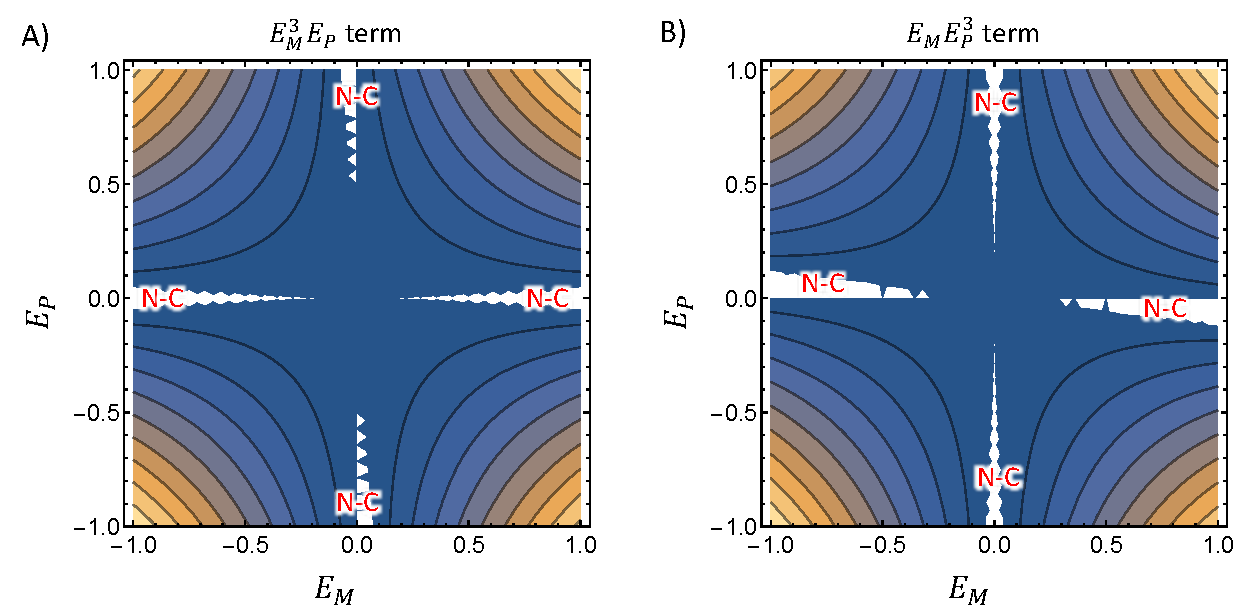
\includegraphics[width=\textwidth]{Images/chapter5/convexitybehavior}
\caption{The criteria for ellipticity (Eqn. \ref{eqn:convexitycriteria}) plotted against the components of the Green-Lagrange strain for A) when including the $E_m^3E_n$ term and B) $E_mE_n^3$ term. The white regions are not convex (N-C), which start at a point along the axes and spreads out as the strain increases.}
\label{fig:convexitybehavior}
\end{figure}
%-------------------	 end FIGURE 	-------------------%
%%%%%%%%%%%%%%%%%%%%%%%%%%%%%%%%%%%%%%%%%%%%%%%%%%%%%%%%%%%%










    
%-----------------------------------------------------------
%	Model scaling for parameter estimation
%-----------------------------------------------------------
\subsection{Model scaling method to improve parameters correlation for parameter estimation} \label{sec:modelscaling}

%-----------------------------------------------------------
%	Computational approaches	
\subsubsection{Parameter correlation for exponential type models}

	One challenging problem with model parameter determination is covariance between the parameters during parameter estimation. Covariance explains how two parameters influence the response of the model and how they will be updated during parameter estimation. High parameter covariance results in both slow convergence and poor reliability and reproducibility of the material parameters. When scaled by the variance, this becomes the correlation between the parameters, with an absolute value between $0$ and $1$. Correlation equal to $1$ implies that two parameters have the exact same effect on the model response, and are thus indistinguishable during parameter estimation. The covariance issue for constitutive models with an exponential function is well described by Aggarwal \cite{aggarwal_inverse_2015, aggarwal_improved_2017}. These constitutive models with exponential functions have a long valley like region in the objective function space. Inside this valley, significantly different parameters produce similar objective function values. This presents several problems. 1) It's difficult to compare model parameters between different specimens, because drastically different parameters can produce similar responses. As such, the average or representative specimen has little real meaning, and each specimen needs to be fitted individually for simulations. 2) The convergence of gradient based optimization algorithms becomes excruciatingly slow due to the small gradients while trapped within this valley. 3) The covariance between parameters being extremely large decreases the accuracy or in other word increases the confidence interval of parameters obtained. 
    
    Aggarwal \textit{et al.} suggested two improvements to alleviate this problem \cite{aggarwal_improved_2017}. These improvements are 1) modifying the modulus parameter $A$ to $e^{a}$, straightening the shape of the valley, and 2) introducing the log-norm for the objective function, improving the gradient along the valley. These modifications have been shown to be effective. However, this is not always ideal. The logarithmic norm suggested faces some issues when fitting stresses or strains, which may be negative and thus becomes undefined. Although this may be alleviated by forgoing data points with negative strains or stresses, but the model may still produce negative values during parameter estimation. Other methods can be used to discard negative values or to take the norm of such values, but these approaches create discontinuities in the gradient of the objective function, causing convergence problems during parameter estimation. Clearly, additional improvements can still be made. 


%-----------------------------------------------------------
%	Scaling method
\subsubsection{Model scaling method}

	We begin by examining the fundamental reason for the high parameter covariance. For this, we will use the 1-D case as an example,
%==========================================================%
%-------------------	begin EQUATION 	-------------------%
\begin{equation}
\begin{aligned}
\Psi &= A \left(e^{B \epsilon} - 1\right) \\
\mathcal{F} &= \sum_i \left(\Psi(\epsilon_i) - \Psi_i \right)^2,
\end{aligned}
\end{equation}
%-------------------	 end EQUATION 	-------------------%
%==========================================================%
where $\Psi$ is the strain energy of our model, $\epsilon$ is some invariant that is a function of the strain, $\epsilon_i$ and $\Psi_i$ are simulated data, and $\mathcal{F}$ is our objective function for parameter estimation. The parameters $A$ and $B$ have different purposes: $A$ is like a modulus, linearly increasing the stiffness of the material, while $B$ modifies the shape of the response, controlling the nonlinearity of the material. However, practically, the two parameters have nearly the same effect on the mechanical response, increasing $A$ increases the stiffness (Fig. \ref{fig:scalingapproach}A) and increasing $B$ also increases the stiffness (Fig. \ref{fig:scalingapproach}B). This is the reason for the high correlation between the parameters (Fig. \ref{fig:scalingapproach}), 0.9979.


%%%%%%%%%%%%%%%%%%%%%%%%%%%%%%%%%%%%%%%%%%%%%%%%%%%%%%%%%%%%
%-------------------	begin FIGURE 	-------------------%
\begin{figure}
\centering
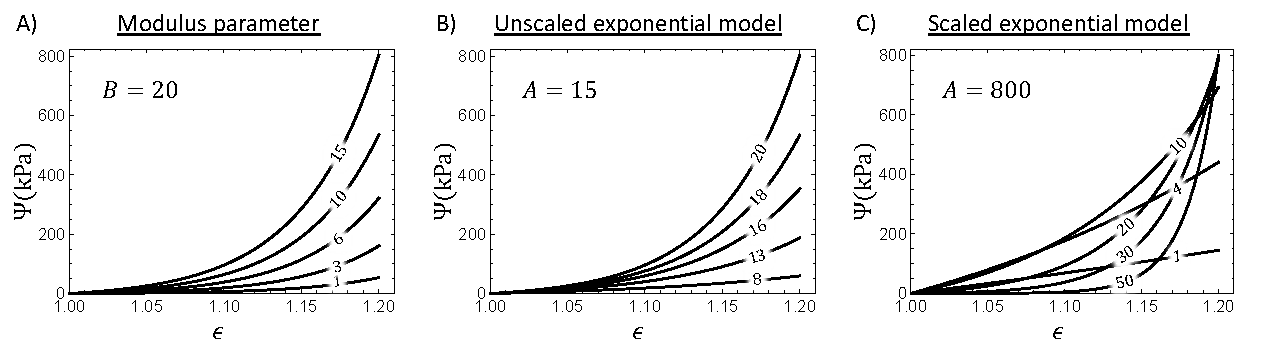
\includegraphics[width=\textwidth]{Images/chapter5/scalingapproach}
\caption{A)The effect of increasing the values of the modulus $A$ on exponential type models. B) The effect of increasing the values of exponent $B$ on exponential type models, which is nearly indistinguishable to the modulus $A$. C) The effect of increasing the values of parameter $B$ after applying the proposed scaling, increasing the values of parameter $A$ remains the same as in A).}
\label{fig:scalingapproach}
\end{figure}
%-------------------	 end FIGURE 	-------------------%
%%%%%%%%%%%%%%%%%%%%%%%%%%%%%%%%%%%%%%%%%%%%%%%%%%%%%%%%%%%%


	To address this problem, we introduce a scaling term to normalize the exponential part of the model, preventing increasing $B$ from increasing the value of the strain energy as a whole, allowing it to only control the curvature. For this, we will use a value $\epsilon_{max}$, which represents the data point with the maximum strain energy value used for parameter estimation, which is also the point where the strain energy stays constant with changes in $B$. The scaled form is thus given by
%==========================================================%
%-------------------	begin EQUATION 	-------------------%
\begin{equation}
\begin{aligned}
\Psi = \Psi_s = \bar{A} \left[e^{-B\epsilon_{max}} \left( e^{B\epsilon} - 1\right)\right],\label{eqn:scaledmodel1D}
\end{aligned}
\end{equation}
%-------------------	 end EQUATION 	-------------------%
%==========================================================%
    where $\bar{A}$ is the scaled version of the modulus $A$. This scaling keeps the exponential part of the model, $e^{-B\epsilon_{max}} ( e^{B\epsilon} - 1)$, at approximately 1.0 at $\epsilon = \epsilon_{max}$, regardless of the changes in the value of the parameter $B$ (Fig. \ref{fig:scalingapproach}C). This effect is not exact when the value of $B$ is small due to the $-1$ needed to set the strain energy to 0 in the referential configuration, but is nonetheless sufficient for our goal: decoupling the modulus increasing effect of the parameter $A$ from the curvature increasing effect of parameter $B$. Indeed, we found this approach to be successful. We examined the contour plot of the objective function with respect to each of the 4 cases in Aggarwal's work \cite{aggarwal_improved_2017}, with the standard objective function, with $A=e^{a}$, with log-norm, and with $A=e^{a}$ and the log-norm, for both without scaling and with scaling (Fig. \ref{fig:objfunctionsurfaces}). First, the correlation between the parameters does not change with $A=e^{a}$. The log-norm improves the correlation from 0.9979 to 0.9063(Table \ref{tb:ABcorrelation}), which significantly improves the objective function surface (Fig. \ref{fig:objfunctionsurfaces}). On the other hand, our scaling method improves the correlation from 0.9979 to 0.6186, more significant than using the log-norm. Interestingly, combining scaling and the log-norm has the adverse effect, increasing the correlation back from 0.6186 to 0.8592. This is a result of essentially linearizing the relation between $A$ and $B$, i.e. from $Ae^{B\epsilon}$ to $Log(A)+B\epsilon$, causing the relationship between $A$ and $B$ to go from modulus and nonlinearity to baseline and modulus. Clearly, \emph{the most optimal parameter estimation approach is to use scaling method with no other modifications}. 
    
    
%%%%%%%%%%%%%%%%%%%%%%%%%%%%%%%%%%%%%%%%%%%%%%%%%%%%%%%%%%%%
%-------------------	begin FIGURE 	-------------------%
\begin{figure}
\centering
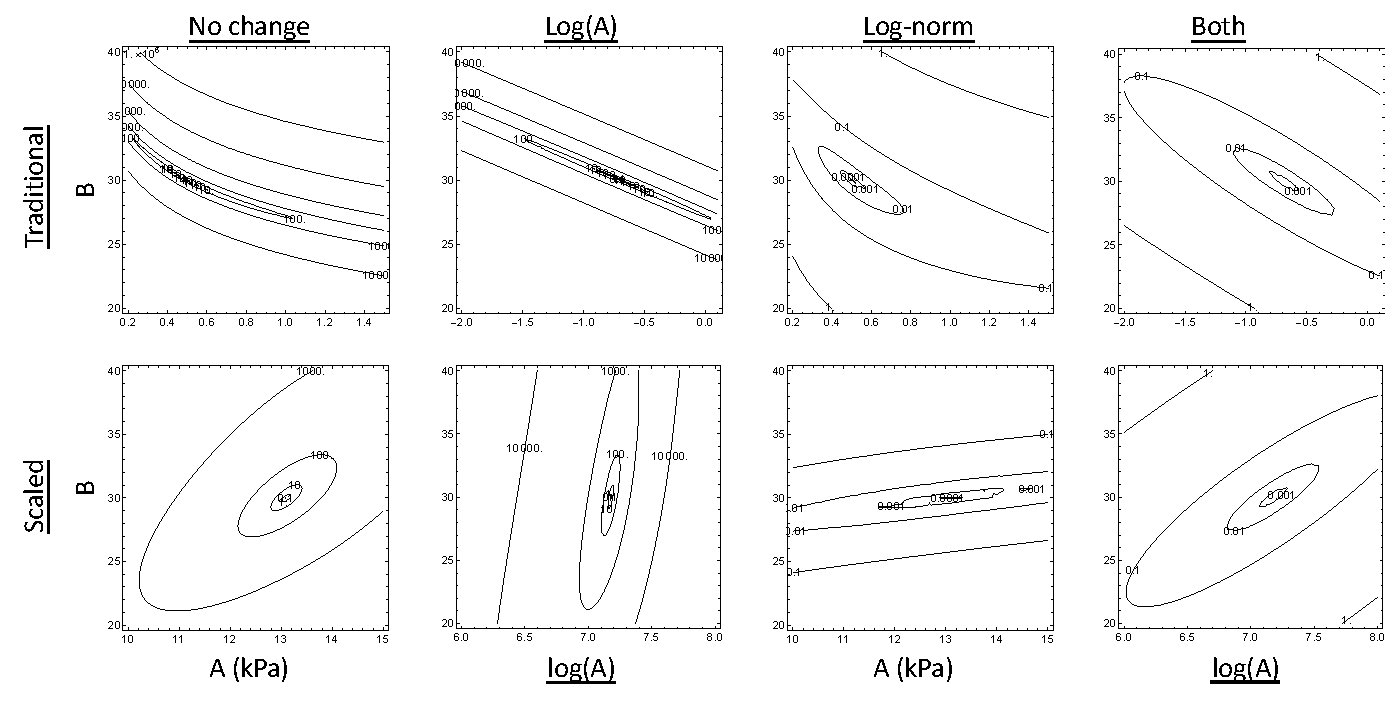
\includegraphics[width=\textwidth]{Images/chapter5/objfunctionsurfaces}
\caption{(Top) The objective function surface for the traditional unscaled exponential models and (Bottom) objective function surface after scaling. From Left to Right are: the unchanged surface, the surface after changing $A$ to $e^{a}$, using the log-norm for the objective function, and applying both changes. The scaled form with no other changes behaves the best.}
\label{fig:objfunctionsurfaces}
\end{figure} 
%-------------------	 end FIGURE 	-------------------%
%%%%%%%%%%%%%%%%%%%%%%%%%%%%%%%%%%%%%%%%%%%%%%%%%%%%%%%%%%%%


%----------------------------------------------------------%
%-------------------	begin TABLE 	-------------------%
\begin{table}
\caption{The correlation between model parameter when using Hencky strains}
\begin{center}
\label{tb:ABcorrelation}
\begin{tabular}{|l|rrrr|}
\hline
			& No change	& $\log(A)$	& $\log$-norm	& Both \\
\hline
Traditional	& -0.9979	& -0.9979	& -0.9063		& -0.9063 \\
Scaled 		& 0.6186	& 0.6186	& 0.8592		& 0.8592 \\
\hline
\end{tabular}
\end{center}
\end{table}
%-------------------	 end TABLE 		-------------------%
%----------------------------------------------------------%



%-----------------------------------------------------------
%	Relation to unscaled form
% \subsubsection{Relation to unscaled model}

    By design, the value of the exponential parameter $B$ does not change by using the scaling method. Since the scaling term does not depend on the input strain, it acts as a modification to the modulus $A$ while keeping the exponential term the same. This also implies that the relationship between the unscaled modulus $A$ and the scaled modulus $\bar{A}$ is
%==========================================================%
%-------------------	begin EQUATION 	-------------------%
\begin{equation}
\begin{aligned}
A = \bar{A} e^{-B\epsilon_{max}},
\end{aligned}
\end{equation}
%-------------------	 end EQUATION 	-------------------%
%==========================================================%
making finding the actual unscaled parameters a simple task. One other benefit of this scaling approach is that the value of $\bar{A}$ is extremely straight forward and intuitive, it is the strain energy of the model at $\epsilon_{max}$. As a result, the value of $\bar{A}$ can be determined \textit{a priori}, or at the very least it is easy to make an initial guess for $\bar{A}$. This will in turn also help to make parameter estimation faster and more accurate, leaving only the parameter $B$ to be determined. 


%-----------------------------------------------------------
%	Extension to multi-variable form
\subsubsection{Extension to multiple variables}

	Extending this method to multiple variables is very simple. For $\Psi_{eff}$ (Eqn. \ref{eqn:finalmodelform}), the input variables become $\mathbf{\epsilon} = \{E_m, E_n, E_\phi\}$, and $\mathbf{\epsilon}_{max} = \{E_m^{max},E_n^{max},E_\phi^{max}\}$. Determining the values for $\mathbf{\epsilon}_{max}$ depends on the form of the objective function. Using the most common case as the example, which is the sum of the squares of the differences in the 2nd Piola Kirchhoff stress,
%==========================================================%
%-------------------	begin EQUATION 	-------------------%
\begin{equation}
\begin{aligned}
\mathcal{F} = \sum_i \left(S_{11}(\epsilon_i) - \hat{S}_{11}^i\right)^2 + \left(S_{12}(\mathbf{\epsilon}_i) - \hat{S}_{12}^i\right)^2 + \left(S_{22}(\epsilon_i) - \hat{S}_{22}^i\right)^2,
\end{aligned}
\end{equation}
%-------------------	 end EQUATION 	-------------------%
%==========================================================%
$\mathbf{\epsilon}_{max}$ is the data point $\mathbf{\epsilon}_i$ which maximizes $\left(\hat{S}_{11}^i\right)^2 + \left(\hat{S}_{12}^i\right)^2 + \left(\hat{S}_{22}^i\right)^2$. 
Thus, we also introduce a $Q_{max}$ such that,
%==========================================================%
%-------------------	begin EQUATION 	-------------------%
\begin{equation} \label{eqn:finalexponentialmodelformscaled}
\begin{aligned}
\Psi_{eff} 	=& c_0 \left(e^{Q} - 1\right) \\
            =& c_0^\prime e^{-Q_{max}}\left(e^{Q} - 1\right)    \\
Q		=& b_1 E_m^2 + b_2 E_n^2 + b_3 E_\phi^2 + b_4 E_m E_n + b_5 E_m^4 + b_6 E_n^4 + b_7 E_m^3 E_n + b_8 E_m^2 E_n^2 + b_9 E_m E_n^3	\\
	&+ b_{10} E_\phi^4 + b_{11} E_m^2E_\phi^2 + b_{12} E_n^2 E_\phi^2 + b_{13} E_m E_n E_\phi^2 \\
Q		=& b_1 (E_m^{max})^2 + b_2 (E_n^{max})^2 + b_3 (E_\phi^{max})^2 + b_4 (E_m^{max}) (E_n^{max}) + b_5 (E_m^{max})^4 + b_6 (E_n^{max})^4   \\ 
    &+ b_7 (E_m^{max})^3 (E_n^{max}) + b_8 (E_m^{max})^2 (E_n^{max})^2 + b_9 (E_m^{max}) (E_n^{max})^3	\\
	&+ b_{10} (E_\phi^{max})^4 + b_{11} (E_m^{max})^2(E_\phi^{max})^2 + b_{12} (E_n^{max})^2 (E_\phi^{max})^2 + b_{13} (E_m^{max}) (E_n^{max}) (E_\phi^{max})^2,
\end{aligned}
\end{equation}
%-------------------	 end EQUATION 	-------------------%
%==========================================================%
where parameter estimation will be done for $c_0^\prime$ instead of $c_0$. Computing the response functions and the stresses, or even the elasticity tensor remains very simple, only requiring multiplying each term by $e^{-Q_{max}}$. Thus, this scaling method is a very simple and easy to implement method of improving the speed and convergence for the parameter estimation of exponential type models. 












%-----------------------------------------------------------
%	Optimal loading paths
%-----------------------------------------------------------
\subsection{Optimal \textit{in silico} loading paths for parameter estimation}\label{sec:optimaldesign}

	Another technique for improving the parameter estimation process for determining $\Psi_{eff}$ from respective micro-models is establishing optimal loading paths. An example is the work of Avazmohammadi \cite{Avazmohammadi2017b}, where optimal experimental design is used to 1) minimize the amount of data necessary and 2) improve model parameter covariance for parameter estimation. Just like one of the most important question to ask before performing any mechanical testing is how much and what kind of data is necessary, we should also be selective with our choice of sampling points for parameter estimation. The theory for optimal design of experiment is well-studied and documented \cite{lanir_optimal_1996, zhu_d_2014}. Vast majority of the methods for optimal design uses D-optimality as the design variable,
%==========================================================%
%-------------------	begin EQUATION 	-------------------%
\begin{equation}\label{eqn:doptimality}
\begin{aligned}
D = \det(\mathbfcal{I}), \quad \mathbfcal{I} = \mathbf{J}^\mathsf{T}\mathbf{J} \quad \mathrm{or} \quad \mathbfcal{I} = \mathbfcal{H},	\\
\mathrm{where} \ J_{ij} = \dpd{f_i}{\xi_j}, \quad \mathcal{H}_{ij} = \dmd{\mathcal{F}}{2}{\xi_i}{}{\xi_j}{},
\end{aligned}
\end{equation}
%-------------------	 end EQUATION 	-------------------%
%==========================================================% 
    where $\mathbf{\xi}$ is a vector of model parameters and $\mathbfcal{I}$ is the information matrix. $\mathbfcal{I}$ can be computed from the derivatives of the objective function $\mathcal{F}$, where $f$ is the model evaluated at each data point, or it can be computed from the Hessian of the objective function, $\mathbfcal{H}$ (Appendix \ref{sec:parametercorrelation}). D-optimality is the determinant of the information or the hessian matrix at the best fit value. It offers the best representation of both parameter accuracy (parameter covariance or correlation) and precision (parameter variance) at the same time.

    
    The first and foremost step is to establish the parameterization for loading paths so they can be optimized. This is not straight a forward choice, as the number of loading path required is not yet established. Another troubling issue is that the number of data points is discrete, thus the gradient of the D-optimality with respect to the control parameters is not smooth. For the sake of time spent for optimization, the number of data points should be kept as small as possible, thus exacerbating the issue of differentiability. Even worse is perhaps that the objective function is essentially flat when not near the optimum, making gradient algorithms not practical. Monte Carlo, random search or divide and conquer strategies are needed, which are much more time consuming. The search space also increases exponentially with the number of loading paths, making a fully exhaustive search difficult to implement. Thus, a simple parameterization for loading paths is ideal. 
    

%%%%%%%%%%%%%%%%%%%%%%%%%%%%%%%%%%%%%%%%%%%%%%%%%%%%%%%%%%%%
%-------------------	begin FIGURE 	-------------------%
\begin{figure}
\centering
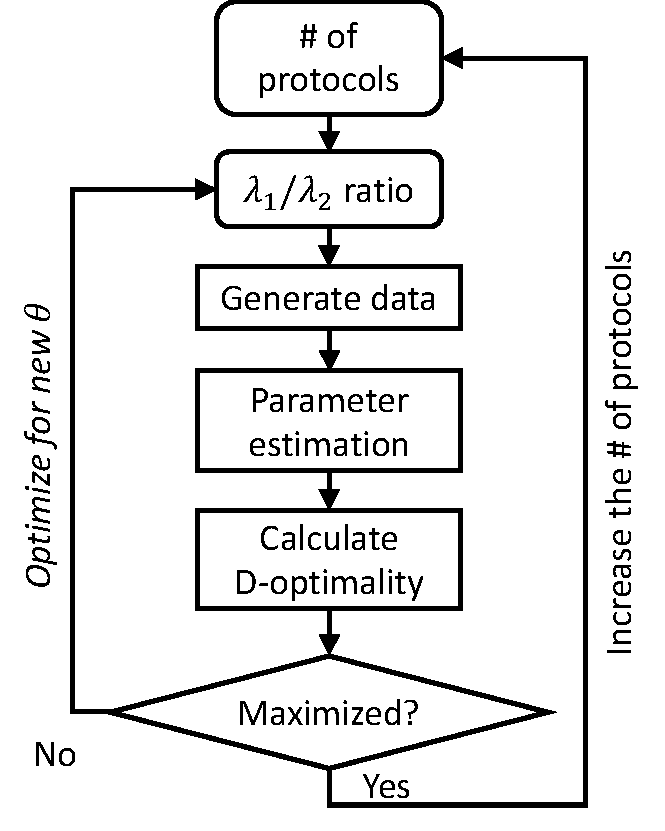
\includegraphics[width=2.5in]{Images/chapter5/optimaldesign}
\caption{Our approach for optimizing for the optimal loading paths for parameter estimation.}
\label{fig:optimaldesign}
\end{figure}
%-------------------	 end FIGURE 	-------------------%
%%%%%%%%%%%%%%%%%%%%%%%%%%%%%%%%%%%%%%%%%%%%%%%%%%%%%%%%%%%%

    
    We define loading paths based on the following conditions: 
\begin{enumerate}
\item The number of loading paths is as small as possible
\item The number of variables needed to define a loading path is as small as possible
\item Possible application to mechanical testing of tissues.
\end{enumerate} 
    Starting with planar extensions only, we chose a loading path as data points which shares the same stretch ratio, $\lambda_1/\lambda_2$, which is typically the same definition used for biaxial mechanical testing. This only requires one constant to be defined for each loading path and the resulting fan shape covers the largest range of deformation with the least number of data points. To determine the optimal loading paths, 1) the total number of loading paths was set, then 2) each combination of the stretch ratios were evaluated for the highst D-optimality (Fig. \ref{fig:optimaldesign}). For a total number of loading paths ranging from 1 to 6, we found the the point when the D-optimality stops increasing significantly, and choose this as the optimal set. Next the shear component, $\kappa_1$, is added. For this study, we constrained the shear to be $0<\kappa_1<0.2$. Only the positive values of $\kappa_1$ is allowed due to the material symmetry. Furthermore, the optimal planar extensions loading paths are always included as a part of the data set.














%%%%%%%%%%%%%%%%%%%%%%%%%%%%%%%%%%%%%%%%%%%%%%%%%%%%%%%%%%%%%
%%  Model Applications										%
%%%%%%%%%%%%%%%%%%%%%%%%%%%%%%%%%%%%%%%%%%%%%%%%%%%%%%%%%%%%%

%-----------------------------------------------------------
%	Use of structural constitutive models
%-----------------------------------------------------------
\subsection{Example application for planar soft tissues}

	The exogenously cross-linked structural model presented in Zhang and Sacks \cite{zhang_modeling_2017} is used to test our approach (Fig. \ref{fig:simulationframework}) and see if $\Psi_{eff}$ (Eqn. \ref{eqn:finalexponentialmodelformscaled}) can completely reproduce its response. This meso-scale structural model is computationally expensive due to integration over the collagen fiber architecture but have been shown to be able to accurately reproduce the mechanical response of a variety of soft tissues, such as mitral valve leaflets \cite{zhang_meso_2016}, ovine pulmonary artery \cite{fata_insights_2014}, myocardium \cite{avazmohammadi_novel_2017}, and exogenously cross-linked bovine pericaridium \cite{sacks_novel_2016}. To briefly summarize, this model is composed of 3 components: collagen, $\Psi_\mathrm{col}$, matrix, $\Psi_\mathrm{mat}$, and interactions, $\Psi_\mathrm{int}$. 
%==========================================================%
%-------------------	begin EQUATION 	-------------------%
\begin{equation}
\Psi 	= \Psi_\mathrm{col} + \Psi_\mathrm{mat} + \Psi_\mathrm{int} \label{eqn:structuralmodelcomponents}
\end{equation}
%-------------------	 end EQUATION 	-------------------%
%==========================================================%
    The matrix term, $\Psi_\mathrm{mat}$, is a modified version of the Yeoh model that is more linear when expressed in 2nd Piola Kirchhoff stress versus stretch, 
%==========================================================%
%-------------------	begin EQUATION 	-------------------%
\begin{equation}\label{eqn:matrixmodel}
\begin{aligned}
\Psi_\mathrm{mat} = &\frac{\eta_M}{2} \left[ \frac{1}{a}\left( I_1 -3\right)^{a} + \frac{r}{b} \left( I_1 -3\right)^{b} \right], \\
&\text{with } 1<a<b, ab <2, 0 \leq r.
\end{aligned}
\end{equation}
%-------------------	 end EQUATION 	-------------------%
%==========================================================%
    This model contains four parameters: $\eta_M$ is the modulus parameter corresponding to the same parameter in the Neo Hookean model, $a$, $b$, and $r$ are the shape parameters, where $a$ and $b$ control the shape of the two terms, while $r$ is the weight between the two terms. In general, $a \approx 1$, $b \approx 1.87$ and $r \approx 15$ can be treated as constants. 


	The response of collagen fibers is given by the integration over the collagen fibers architecture, their orientation and crimp. The fiber orientations is described by a beta distribution function and fiber crimp is described by another beta distribution function of the stretches needed to straighten the fibers, the slack stretch $\lambda_s$. These are referred to as the orientation distribution function (ODF), $\Gamma$, and the recruitment distribution function (RDF), $D$, respectively, with the forms given in Zhang and Sacks \cite{zhang_meso_2016, zhang_modeling_2017, sacks_novel_2016}. The form of the strain energy function is 
%==========================================================%
%-------------------	begin EQUATION 	-------------------%
\begin{equation} \label{eqn:collagen}
\begin{aligned}
\Psi_\mathrm{col} =& \phi_\mathrm{col} \eta_C \int\displaylimits_\theta \Gamma(\theta) 
\int\displaylimits_1^{\lambda_\theta} D\left(\lambda_s \right) \left( \frac{\lambda_\theta}{\lambda_s} - 1\right)^2 \mathrm{d}\lambda_s \mathrm{d}\theta,
\end{aligned}
\end{equation}
%-------------------	 end equation 	-------------------%
%----------------------------------------------------------%
    where $\eta_C$ is the modulus of the collagen fibers, $\lambda_\theta = \sqrt{\mathbf{n}_\theta \cdot \mathbf{C}\mathbf{n}_\theta}$ is the stretch of the ensemble of collagen fiber with the same orientation, and $\lambda_\mathrm{\theta}/\lambda_s$ is the true stretch of the collagen fibers after they are straightened \cite{zhang_meso_2016}. Similarly, the response of the interaction term is given by integration over pairs of fibers based on their orientation and crimp, which contains a quadruple integral. 
%==========================================================%
%-------------------	begin EQUATION 	-------------------%
\begin{equation}
\Psi_\mathrm{int} = \frac{\eta_I}{2} \int\displaylimits_\alpha \int\displaylimits_\beta \Gamma(\alpha) \Gamma(\beta) \int\displaylimits_1^{\lambda_\alpha} \int\displaylimits_1^{\lambda_\beta} D\left( x_\alpha \right) D\left( x_\beta \right) \left( \frac{\lambda_\alpha \lambda_\beta}{x_\alpha x_\beta} - 1\right)^2 \,\mathrm{d}x_\alpha \,\mathrm{d}x_\beta \,\mathrm{d}\alpha \,\mathrm{d}\beta.
\end{equation}
%-------------------	 end EQUATION 	-------------------%
%==========================================================%
For clarity of presentation, the slack stretches, $\lambda_s$, are replaced by $x_\alpha$ and $x_\beta$ for fiber oriented along the angle $\alpha$ and $\beta$ respectively. Only one parameter, the modulus $\eta_I$, is used to account for all interactions, with the same $\Gamma$ and $D$ already given above. 

The second Piola Kirchhoff stress, $\mathbf{S}=2\frac{\partial\Psi}{\partial\mathbf{C}}$, is 
%==========================================================%
%-------------------	begin EQUATION 	-------------------%
\begin{equation} \label{eqn:fullcollagen}
\begin{aligned}
\mathbf{S} = & \phi_\mathrm{col} \eta_C \int\displaylimits_\theta \Gamma(\theta)\left\lbrace 
\int\displaylimits_1^{\lambda_\theta} \frac{D\left( x \right)}{x} \left( \frac{1}{x}- \frac{1}{\lambda_\theta}\right) \mathrm{d}x \right\rbrace \mathbf{n}_\theta\otimes\mathbf{n}_\theta \mathrm{d}\theta \\
+ & \phi_\mathrm{col} \eta_I \int\displaylimits_\alpha \int\displaylimits_\beta \Gamma \left(\alpha \right) \Gamma \left( \beta \right) \\
& \times \left[ \left\lbrace 
\int\displaylimits_1^{\lambda_\alpha} \int\displaylimits_1^{\lambda_\beta} 
\frac{2 \lambda_\beta D(x_\alpha) D(x_\beta)}{x_\alpha x_\beta} 
\left( \frac{\lambda_\alpha}{x_\alpha} \frac{\lambda_\beta}{x_\beta} - 1\right) \mathrm{d}x_\alpha \, \mathrm{d}x_\beta 
+\int\displaylimits_1^{\lambda_\beta} D(x_\beta) \left( \frac{\lambda_\beta}{x_\beta} -1  \right)^2 \mathrm{d}x_\beta \right\rbrace \right.  \frac{\mathbf{n}_\alpha \otimes \mathbf{n}_\alpha}{\lambda_\alpha}  \\
& + \left. \left\lbrace
\int\displaylimits_1^{\lambda_\alpha} \int\displaylimits_1^{\lambda_\beta} 
\frac{2 \lambda_\alpha D(x_\alpha) D(x_\beta)}{x_\alpha x_\beta} 
\left( \frac{\lambda_\alpha}{x_\alpha} \frac{\lambda_\beta}{x_\beta} - 1\right) \mathrm{d}x_\alpha \, \mathrm{d}x_\beta 
+ \int\displaylimits_1^{\lambda_\alpha} D(x_\alpha) \left( \frac{\lambda_\alpha}{x_\alpha} -1  \right)^2 \mathrm{d}x_\alpha \right\rbrace \frac{\mathbf{n}_\beta \otimes \mathbf{n}_\beta}{\lambda_\beta}  \right] \mathrm{d}\alpha \, \mathrm{d}\beta\\
+ & \phi_\mathrm{mat} \eta_M \left[\left(\left( I_1 - 3\right)^{a - 1} + r \left( I_1 - 3\right)^{b - 1}\right) \left( \mathbf{I} - C_{33}\mathbf{C}^{-1}\right)  \right],\\
\end{aligned}
\end{equation}
%-------------------	 end EQUATION 	-------------------%
%==========================================================%
    where $\phi_\mathrm{col}$ and $\phi_\mathrm{mat}$ are the mass fraction of collagen and matrix respectively. 
    
	Although very accurate and predictive, this model is not only computationally expensive, numerical integration also results in a significant decrease in numerical precision when the number of quadrature point is insufficient. This can create a number of issues for convergence during parameter optimization. Thus, the implementation of this model is complicated by a constant balance between computational cost and numerical robustness during optimization. Using $\Psi_{eff}$ to reproduce its response is a solution to these issues. Furthermore, some modifications can be made to reduce the form of $\psi_{eff}$ based on how well each term captures the behavior of the respective material (see Appendix \ref{sec:specificform}).
    
    
    



	









%-----------------------------------------------------------
%	Parameter estimation
%-----------------------------------------------------------
\subsection{Parameter estimation}

	The objective function we use is 
%==========================================================%
%-------------------	begin EQUATION 	-------------------%
\begin{subequations}\label{eqn:objectivefunction}
\begin{gather}
S_m = \dpd{\Psi}{E_m} = \mathbf{m}_0\cdot\mathbf{S}\mathbf{m}_0,
	\quad S_n = \dpd{\Psi}{E_n} = \mathbf{n}_0\cdot\mathbf{S}\mathbf{n}_0,
    \quad S_\phi = \dpd{\Psi}{E_\phi} = 2\mathbf{m}_0\cdot\mathbf{S}\mathbf{n}_0 \label{eqn:responsefunctions}\\
\mathcal{F} = \sum_i^n \left(S_m(\hat{E}_M^i, \hat{E}_S^i, \hat{E}_\phi^i) - \hat{S}_M^i \right)^2 + \left(S_n(\hat{E}_M^i, \hat{E}_S^i, \hat{E}_\phi^i) - \hat{S}_S^i \right)^2 + \left(S_\phi(\hat{E}_M^i, \hat{E}_S^i, \hat{E}_\phi^i) - \hat{S}_\phi^i \right)^2
\end{gather}
\end{subequations}
%-------------------	 end EQUATION 	-------------------%
%==========================================================%
    This removes rigid body rotation and puts the stresses along the material axes, giving the response functions and minimizes covariance between the parameters during optimization. Other possible options include the log of the L2-norm, the log-norm presented by Aggarwal \cite{aggarwal_improved_2017}, and L2-norm of the strain energy and other stresses.


	For optimal speed, gradient methods are ideal. Because we require some non-linear constraints to enforce convexity, we utilized the interior point algorithm provided by the IPOPT library \cite{waechter_implementation_2005}. The initial guess is easily derived for the model scaling method, with the parameter $c_0$ being the maximum strain energy in the available data. The exponent parameters $b_i$ are generally very consistent in value, with the quadratic parameters being $b_1 \approx 10$, $b_2 \approx 10$, and $b_4 \approx -10$, the quartic parameters being $b_5 \approx 2000$, $b_6 \approx 500$, $b_9 \approx 200$, $b_{10} \approx 200$, $b_{11} \approx 200$, $b_{12} \approx 200$. We find this setup to work extremely well, and no further modification being necessary. 




\subsection{Reproducing the response of soft tissues using the effective constitutive model and optimal loading paths}\label{sec:reproducefung}

	For our approach (Fig. \ref{fig:simulationframework}), we need to overcome the limitation of common phenomenological approaches on predicting the mechanical response of micro-models outside of the data set used for parameter estimation \cite{sun_biaxial_2003}. To verify this, we will first reproduced the results of Sun \textit{et al.} \cite{sun_biaxial_2003} using the generalized Fung model, then repeat the process using $\Psi_{eff}$ (Eqn. \ref{eqn:finalexponentialmodelformscaled}) with optimal loading paths. We will focus on glutaraldehyde cross-linked bovine pericardium as the tissue. Bovine pericardium is the most common material used to fabricate bioprosthetic heart valves. It is extremely dense in collagenous fibers, having broad fiber splays with approximately $30\deg$ in standard deviation. The resulting mechanical behavior have strong coupling between the axial stretches. Thus, the mechanical response of some bovine pericardium specimens are fitted to the structural model (Eqn. \ref{eqn:fullcollagen}). The structural model is then used to generate stress strain data along loading paths with stress ratios ($S_{11}/S_{22}$) of $0.1:1$, $0.5:1$, $0.75:1$, $1:1$, $1:0.75$, $1:0.5$, and $1:0.1$. Following Sun \textit{et al.} \cite{sun_biaxial_2003}, the generalized Fung model (Eqn. \ref{eqn:generalizedfungmodela}) was fitted to the five loading paths in the physiologic range ($0.5:1$, $0.75:1$, $1:1$, $1:0.75$, $1:0.5$), then the remain two loading paths were predicted and compared to the data. Next, the reverse scenario was done, where the generalized Fung model was fitted to the non-physiologic loading paths ($0.1:1$ and $1:0.1$), while the remaining five loading paths were predicted. Following the same step, $\Psi_{eff}$ was fitted to the three optimal loading paths ($0.1:1$, $1:1$, and $1:0.1$) while the remaining loading paths were predicted. 
    
    We also considered some alternative loading paths. In the original paper by Fung et al. on the constitutive modeling of arteries \cite{fung_pseudoelasticity_1979}, they discussed the use of 'physiologic protocols' as the optimal data set for parameter estimation. These 'physiologic protocols' are loading paths that cover a range past some predetermined lower bounds for $E_{11}$ and $E_{22}$. Conceptually, this is meant to correspond to the range after accounting for the prestrain between the zero stress configuration and the \textit{in vivo} unloaded (not stress free) configuration. For clarity, to distinguish between this and the physiologic range (the range where the physiologic loading path is likely to reside) in Sun \textit{et al.}, we will refer to this as the prestrained range. We reproduced the prestrained protocols in figure 5 of Fung \textit{et al.} \cite{fung_pseudoelasticity_1979}, and compared the results to those with optimal loading paths. 





\subsection{Numerical simulations}

	An exhaustive numerical study using $\Psi_{eff}$ (Eqn. \ref{eqn:finalexponentialmodelformscaled}) is beyond the scope of this work. However, we hereby present an example implementation of the framework we proposed (Fig. \ref{fig:simulationframework}) using $\Psi_{eff}$ (Eqn. \ref{eqn:finalexponentialmodelformscaled}) to homogenize the structural model (Eqn. \ref{eqn:fullcollagen}) for facilitating numerical simulation of intact bioprothetic heart valves. The leaflet material consider are bovine pericardium (most commonly used for bioprothetic heart valve leaflets), porcine aortic valve (highly anisotropy response), and bovine pericardium with an uniform fiber ODF (isotropic). We replicated the response of these tissues using the structural model based on their microstructure. We then fit $\Psi_{eff}$ to the structural model by sampling along optimal loading paths. Next, we evaluated the computational cost and numerical robustness of $\Psi_{eff}$ and its ability to handle a wide range of material properties and the complex \textit{in vivo} deformations in numerical simulations.
    
    
    For numerical simulation, we utilized the custom finite element simulation software developed by Hsu \textit{et al.} \cite{hsu_dynamic_2015, kamensky_immersogeometric_2015, kiendl_isogeometric_2015, wu_anisotropic_2018}. Briefly, the finite element code was developed for isogeometric fluid solid dynamics simulation of heart valves, focusing mostly on the tri-leaflet atrioventricular valves. The tri-leaflet geometry is based on the commonly used Edwards Pericardial Heart Valve with Kirchhoff-Love shells for the leaflets \cite{kiendl_isogeometric_2015} and finite element solver developed in by Kamensky \textit{et al.} \cite {kamensky_immersogeometric_2015}. We utilized this code to simulate leaflet deformation under physiological quasi--static transvalvular pressure. 
    A total was 484 B\'ezier elements was used for each leaflets, with a leaflet density of 1.0 g/cm$^3$ and a uniform leaflet thickness of 0.386mm thick \cite{hsu_dynamic_2015}. Contact between leaflets is handled by a penalty-based approach and imposed at quadrature points of the shell structure, and clamped boundary condition is applied to the leaflet attachment edge. 
    For simplicity and consistency, the collagen fiber direction was assume to be aligned to the circumferential direction of each leaflet. No root, atrial chamber or the surrounding artery was used. The bioprothetic heart valve stent was made rigid and undeformable, serving a stationary reference for the leaflets. A similar validation process to the one presented by Wu \textit{et al.} \cite{wu_anisotropic_2018} to verify the implementation.


%---    Results
\section{Results}

%%%%%%%%%%%%%%%%%%%%%%%%%%%%%%%%%%%%%%%%%%%%%%%%%%%%%%%%%%%%%
%%  Optimal loading paths for parameter estimation  %%%%%%%%%

\subsection{Optimal \textit{in silico} loading paths for parameter estimation}

	The optimal loading paths for reproducing the response of dense collagenous soft tissues such as bovine pericardium and porcine aortic valve consist of 8 loading paths (Fig. \ref{fig:doptimality}C): 5 loading paths consisting of only inplane extensions (Fig. \ref{fig:doptimality}D), and 3 with the addition of the shear component. The increase in D-optimality is significantly less after three loading paths for the in-plane extensions (Fig. \ref{fig:doptimality}A). Same is true for the loading paths with shear. These three loading paths are the equibiaxial stress (Fig. \ref{fig:doptimality}B, Blue), and two uniaxial loading paths (Black, Green). The type of stress is consistent with the stress used for parameter estimation. The loading paths with shear simply iterates on these three loading paths by adding the shear component, we specified the maximum strain to be applied to be $0.2$. We consider this to be the minimal number of loading paths necessary for parameter estimation. In practice, it's better to add the intermediate inplane tension loading paths (Red, Orange) as a precaution, forming the full set of 8 loading paths (Fig. \ref{fig:doptimality}C). 
	
	
	The equi-biaxial stress loading path is the most important loading path. The D-optimality is $10^{-17}$ for the equi-biaxial loading path versus less than $10^{-300}$ (using \textit{Mathematica}'s extended precision) for other loading paths. The set of optimal loading paths will always contain the equi-biaxial stress loading path if the total number is odd, whereas it will always contain two loading paths just beside the equi-biaxial loading paths if it is even. The other loading paths complement the equi-biaxial loading path by spanning the range being searched. More details on the optimal loading path results are presented in appendix \ref{sec:optimalpaths}.
	
%-------------------	begin FIGURE 	-------------------%
\begin{figure}[hbtp]
\centering
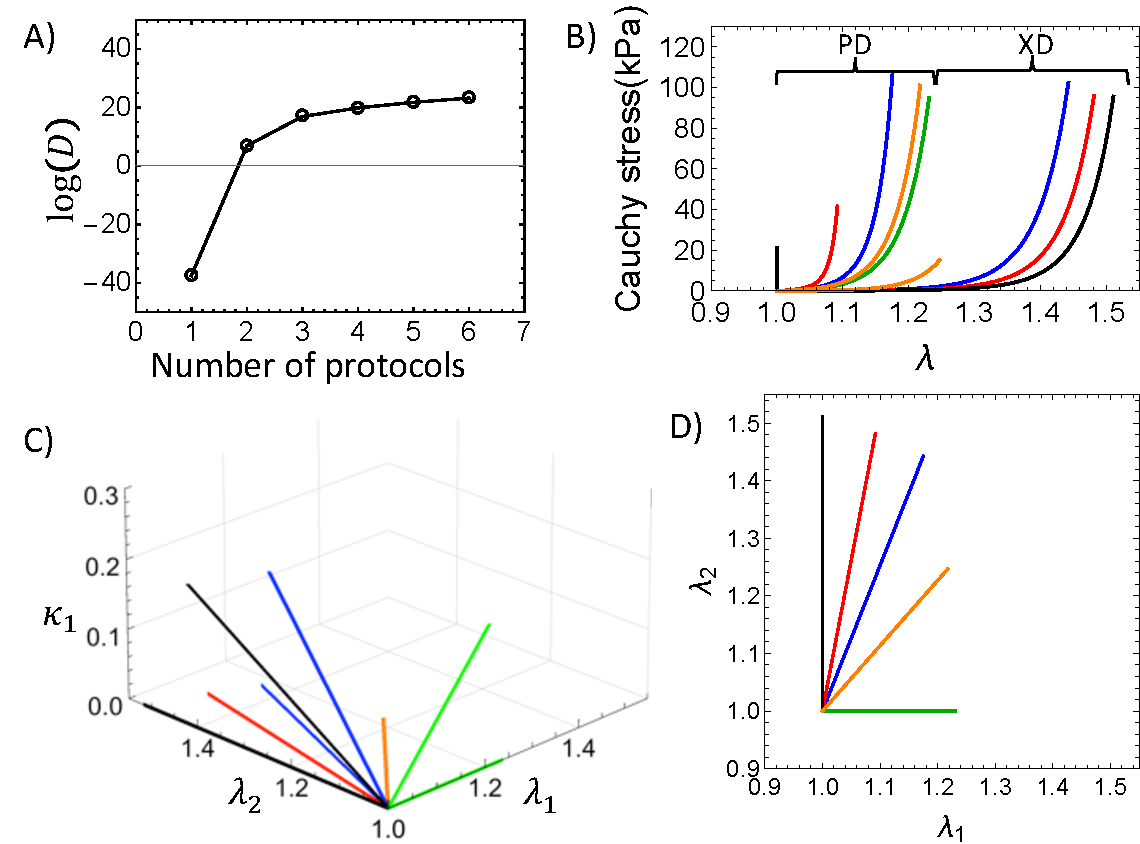
\includegraphics[width=5.5in]{Images/chapter5/doptimality}
\caption{A) The best D-optimality value for a given number of loading paths used to generate the data, which stops increasing significantly after three. B) The stress-strain curve of the optimal set of five loading paths with no shear. C) The full set of optimal loading paths including the shear component are shown. The same colored loading paths are built upon the corresponding D) planar stretch loading paths by adding a shear component. }
\label{fig:doptimality}
\end{figure} 
%-------------------	 end FIGURE 	-------------------%









%%%%%%%%%%%%%%%%%%%%%%%%%%%%%%%%%%%%%%%%%%%%%%%%%%%%%%%%%%%%%
%%  Parameter estimation and the quality of fit             %

\subsection{Parameter estimation and the quality of fit}

    The time taken for parameter estimation (5-10 seconds) is significantly lower in comparison to meso-scale structural approaches, such for the mitral valve \cite{zhang_meso_2016} (10-40 minutes) and exogenously crosslinked tissues \cite{zhang_modeling_2017}(30 min - 4 hours). In addition, we found that the model scaling method significantly improves the consistency of convergence. Parameters converges in approximately 40-60 iterations regardless of starting point, whereas it can vary between 40-120 iterations without using scaling. The additional iterations occur within the valley like region in the objective function surface (Fig. \ref{fig:objfunctionsurfaces}), where the gradient and thus the step size is very small. Of course, we found both methods to be essentially equivalent with a sufficiently good initial guess. We note that the model scaling method does not improve the correlations between the exponent parameters $b_1-b_{13}$ in $Q$. With that being said, the correlations between the exponent parameters $b_1-b_{13}$ are significantly better than the correlations between these exponents and modulus $c_0$ (Fig. \ref{fig:gvsecorrelation} and Appendix \ref{sec:parametercorrelation} Table \ref{tb:correlationE} \& \ref{tb:correlationG} vs. Table \ref{tb:ABcorrelation}), which is not much of a problem for parameter estimation. It is difficult to further improve the parameter correlation of $Q$ without changing the form of the model, but, for our purpose, this is already sufficient. 
    
    
    Qualitatively, $\Psi_{eff}$ (Eqn. \ref{eqn:finalexponentialmodelformscaled}) matches the response of collagenous soft tissues reproduced using the structural model (Eqn. \ref{eqn:fullcollagen}). It is able to follow all the characteristics of the response function (derivatives of the strain energy density function), including the symmetry with respect to shear (Fig. \ref{fig:modelfit}). The average $R^2$ is 0.958 (n = 6) for the bovine pericardium specimens tested. We found similar values for porcine aortic valve leaflets. The main improvements are in the uniaxial strain regions. 
%-------------------	begin FIGURE 	-------------------%
\begin{figure}[hptb]
\centering
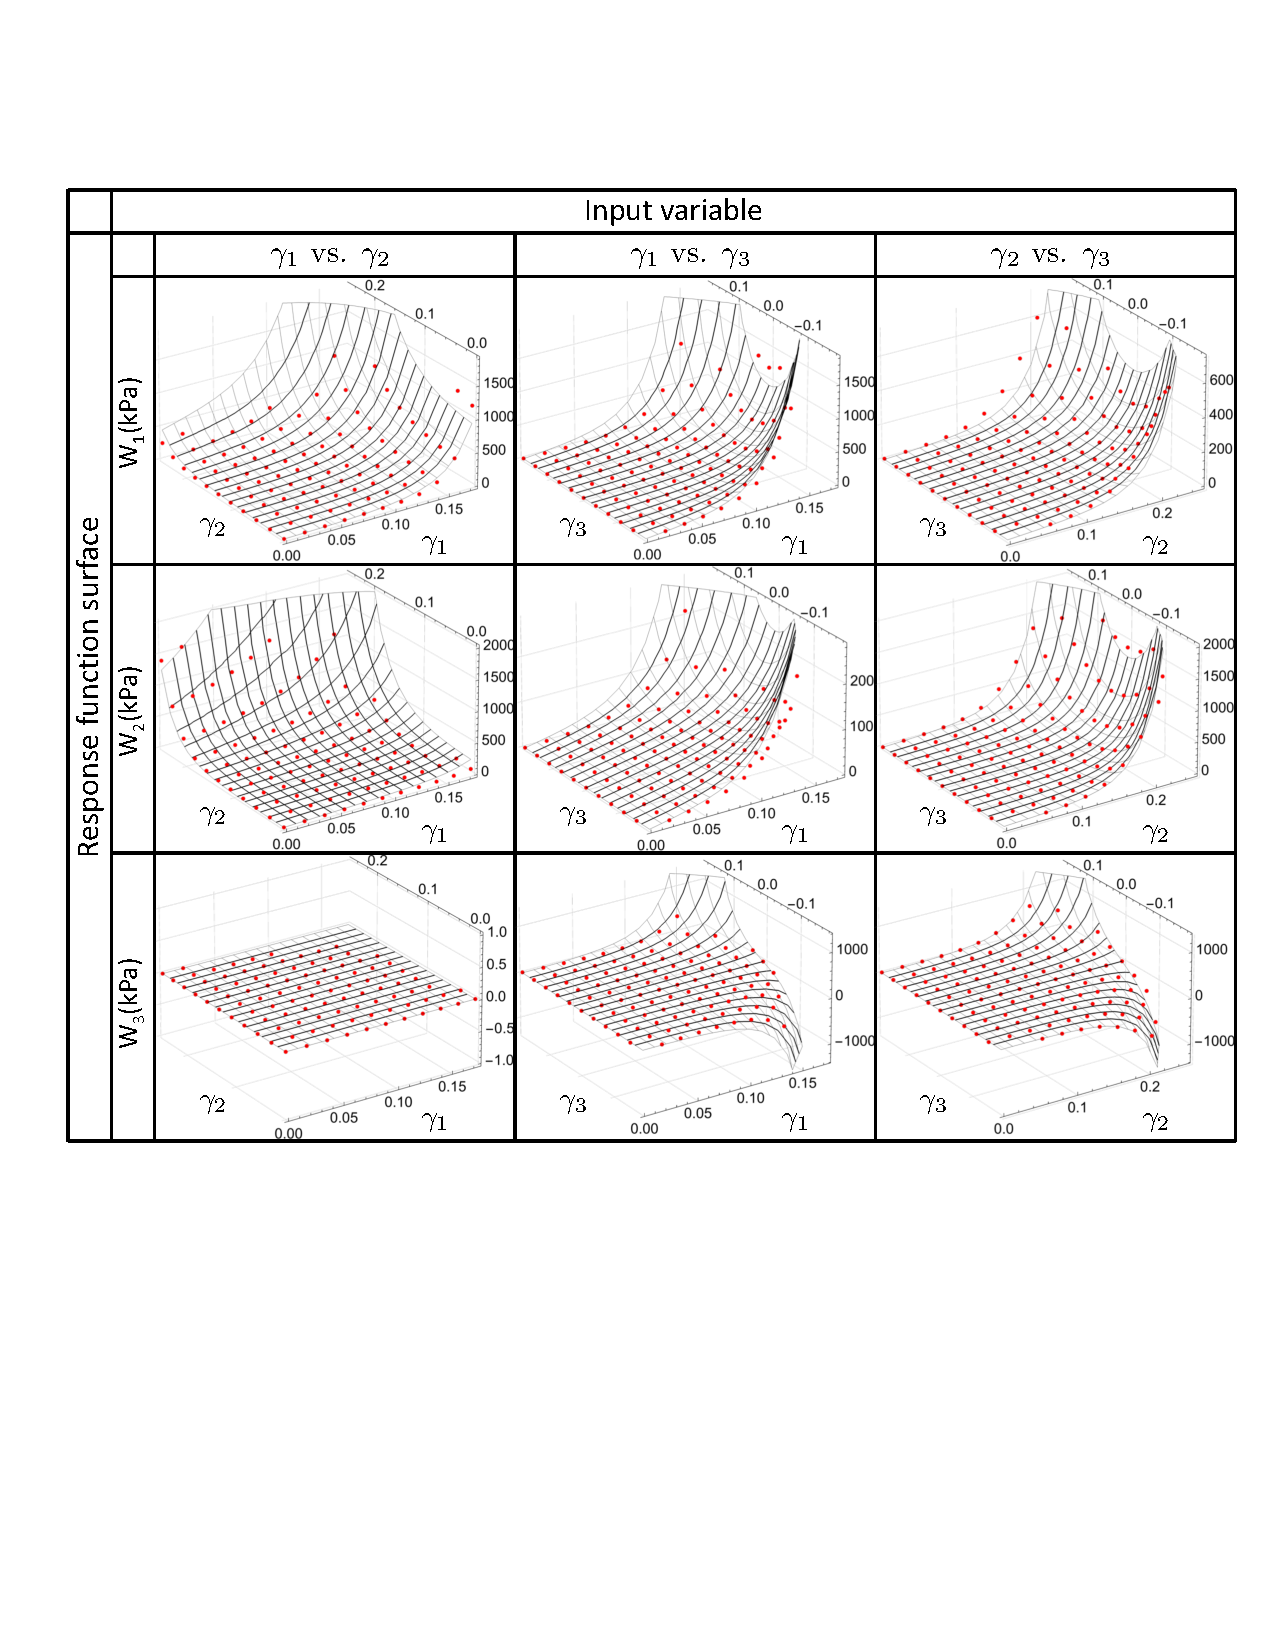
\includegraphics[width=\textwidth]{Images/chapter5/modelfit}
\caption{Parameter estimation results showing that $\Psi_{eff}$ is able to replicate the response function of the structural model (Eqn. \ref{eqn:objectivefunction}) (Top) $S_m = \partial\Psi/\dif E_m$, (Middle) $S_n = \partial\Psi/\dif E_n$, and (Bottom) $S_\phi = \partial\Psi/\dif E_\phi$ for each pair of Green Lagrange strain components.}
\label{fig:modelfit}
\end{figure} 
%-------------------	 end FIGURE 	-------------------%


    For a more detailed comparison, we replicated the result of Sun \textit{et al.} \cite{sun_biaxial_2003}. Similarly, we found that the generalized Fung model (Eqn. \ref{eqn:generalizedfungmodela}) fitted the five loading paths in the physiologic range very well (Fig. \ref{fig:fungphyfit}), but predicted the remaining unfitted loading paths poorly (Fig. \ref{fig:fungphypred}). When the non-physiologic loading paths are fit ((Fig. \ref{fig:fungphyfit})), the remaining protocols are still predicted poorly. However, we do note here that the generalized Fung model cannot fit the non-physiologic protocols very well, illustrating the limitation of the generalized Fung model at fitting the response of soft tissue in a wide range of deformations (Section \ref{sec:possibleforms}). 

%%%%%%%%%%%%%%%%%%%%%%%%%%%%%%%%%%%%%%%%%%%%%%%%%%%%%%%%%%%%
%-------------------	begin FIGURE 	-------------------%
\begin{figure}[hptb]
\centering
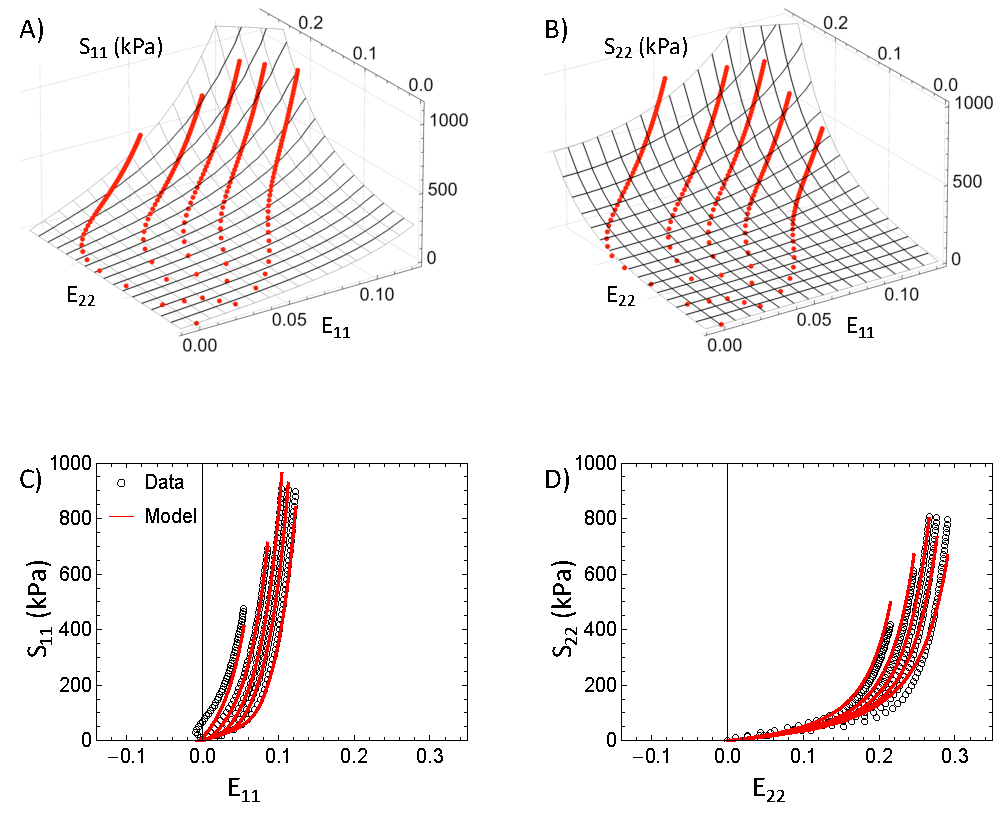
\includegraphics[width=\textwidth]{Images/chapter5/fungphyfit}
\caption{Reproducing the results of Sun \textit{et al.} \cite{sun_biaxial_2003} showing that the generalized Fung model is able to fit the loading paths in the physiologic range very well. A) The $S_{11}$ surface fitted to the data points. B) The $S_{22}$ surface fitted to the data points. C) Best fit of the $S_{11}$ component of the loading paths. D) Best fit of the $S_{22}$ component of the loading paths.}
\label{fig:fungphyfit}
\end{figure} 
%-------------------	 end FIGURE 	-------------------%
%%%%%%%%%%%%%%%%%%%%%%%%%%%%%%%%%%%%%%%%%%%%%%%%%%%%%%%%%%%%

%%%%%%%%%%%%%%%%%%%%%%%%%%%%%%%%%%%%%%%%%%%%%%%%%%%%%%%%%%%%
%-------------------	begin FIGURE 	-------------------%
\begin{figure}[hptb]
\centering
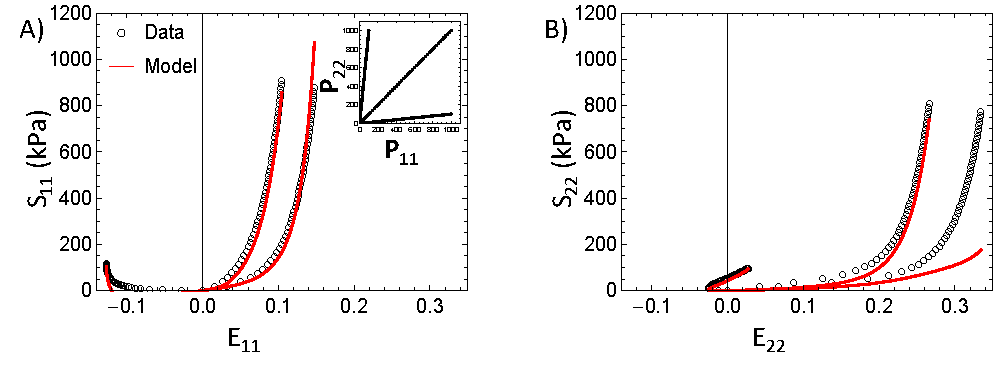
\includegraphics[width=\textwidth]{Images/chapter5/fungphypred}
\caption{Reproducing the results of Sun \textit{et al.} \cite{sun_biaxial_2003} showing the A) $S_{11}$ component and B) $S_{22}$ component of the remaining unfitted loading paths are predicted poorly from fit (Fig. \ref{fig:fungphyfit}). The inset in A shows the corresponding loading paths.}
\label{fig:fungphypred}
\end{figure} 
%-------------------	 end FIGURE 	-------------------%
%%%%%%%%%%%%%%%%%%%%%%%%%%%%%%%%%%%%%%%%%%%%%%%%%%%%%%%%%%%%


%%%%%%%%%%%%%%%%%%%%%%%%%%%%%%%%%%%%%%%%%%%%%%%%%%%%%%%%%%%%
%-------------------	begin FIGURE 	-------------------%
\begin{figure}[hptb]
\centering
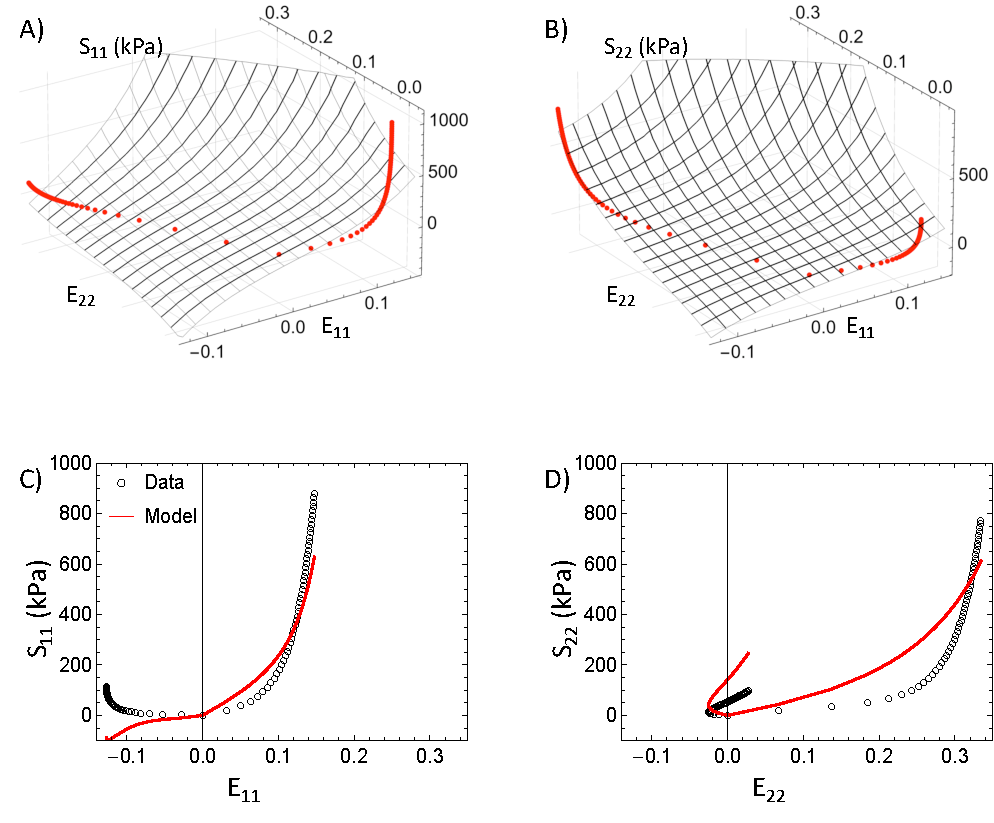
\includegraphics[width=\textwidth]{Images/chapter5/fungoutfit}
\caption{Reproducing the results of Sun \textit{et al.} \cite{sun_biaxial_2003} showing the best fit of the generalized Fung model to the loading paths in the non-physiologic range is poor. A) The $S_{11}$ surface fitted to the data points. B) The $S_{22}$ surface fitted to the data points. C) Best fit of the $S_{11}$ component of the loading paths. D) Best fit of the $S_{22}$ component of the loading paths.}
\label{fig:fungoutfit}
\end{figure} 
%-------------------	 end FIGURE 	-------------------%
%%%%%%%%%%%%%%%%%%%%%%%%%%%%%%%%%%%%%%%%%%%%%%%%%%%%%%%%%%%%

%%%%%%%%%%%%%%%%%%%%%%%%%%%%%%%%%%%%%%%%%%%%%%%%%%%%%%%%%%%%
%-------------------	begin FIGURE 	-------------------%
\begin{figure}[hptb]
\centering
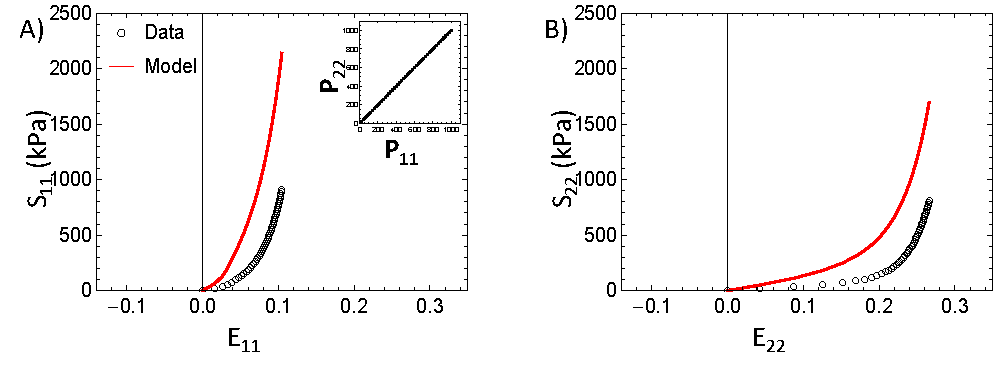
\includegraphics[width=\textwidth]{Images/chapter5/fungoutpred}
\caption{Reproducing the results of Sun \textit{et al.} \cite{sun_biaxial_2003} showing the A) $S_{11}$ component and B) $S_{22}$ component of the equi-biaxial stress loading path are predicted poorly from fit (Fig. \ref{fig:fungoutfit}). The inset in A shows the corresponding loading paths.}
\label{fig:fungoutpred}
\end{figure} 
%-------------------	 end FIGURE 	-------------------%
%%%%%%%%%%%%%%%%%%%%%%%%%%%%%%%%%%%%%%%%%%%%%%%%%%%%%%%%%%%%
    

	Using $\Psi_{eff}$ (Eqn. \ref{eqn:finalexponentialmodelformscaled}) (Fig. \ref{fig:effphyfit}) improves these results, but using non-optimal loading paths, such as based on Fung \textit{et al.}'s prestrained protocols \cite{fung_pseudoelasticity_1979}, lead to poor predictions for other loading paths (Fig. \ref{fig:effphypred}). Although not obvious at first, $\Psi_{eff}$ severely underestimates the response of the material in the low stress region. The D-optimality with two protocols in this prestrained range is only $1.35$, which improves to $1.98\times 10^4$ with six protocols. This pales in comparison to $9.7 \times 10^2$ for the two optimal protocols and $2.2 \times 10^7$ with three optimal protocols. When both $\Psi_{eff}$ and three optimal loading paths are utilized, we found that the loading paths are both fitted (Fig. \ref{fig:effoptfit}) and predicted very well (Fig. \ref{fig:effoptpred}). We also tested other non-optimal loading paths with modifications to the form of $\Psi_{eff}$ (Appendix \ref{sec:otherresults}). To briefly summarize these results, with an optimal set of loading paths, $\Psi_{eff}$ is able to fully reproduce the response of collagenous soft tissue for a wide range of deformation. However, without optimal loading paths, the form of $\Psi_{eff}$ can have unpredictable impact on the predicted response, even though the quality of fit is very similar. 


%%%%%%%%%%%%%%%%%%%%%%%%%%%%%%%%%%%%%%%%%%%%%%%%%%%%%%%%%%%%
%-------------------	begin FIGURE 	-------------------%
\begin{figure}[hptb]
\centering
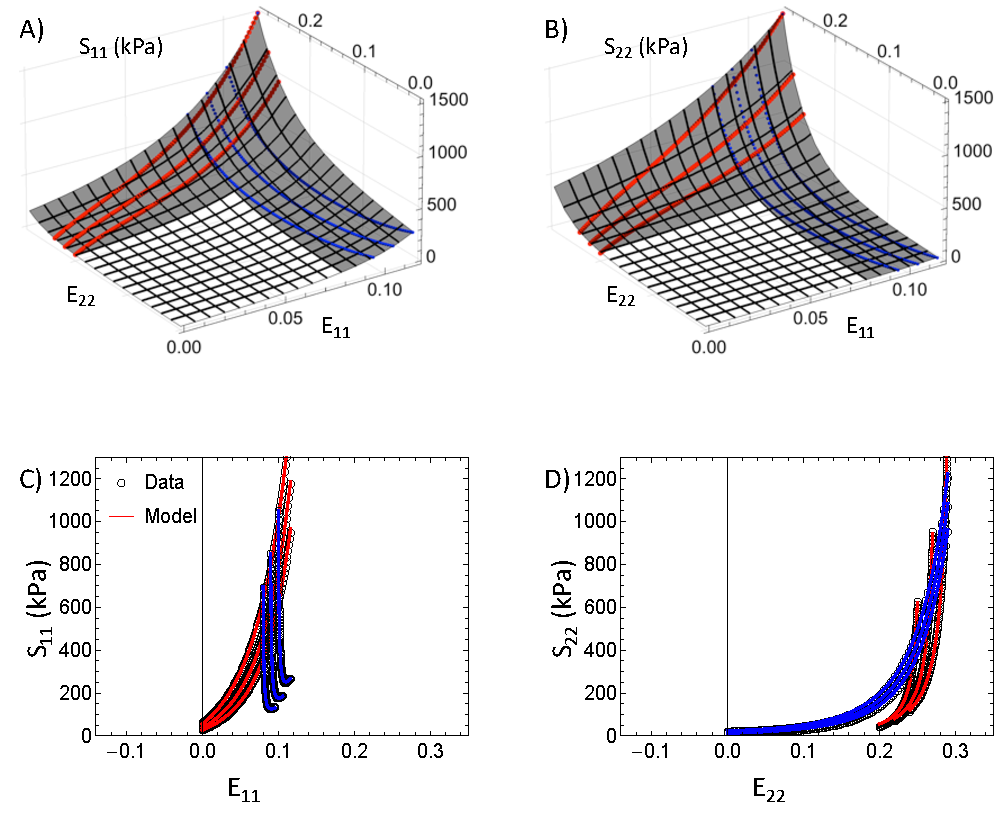
\includegraphics[width=\textwidth]{Images/chapter5/effphyfit}
\caption{The fit of $\Psi_{eff}$ to the prestrained loading paths is very good. A) The $S_{11}$ surface fitted to the data points. B) The $S_{22}$ surface fitted to the data points. C) Best fit of the $S_{11}$ component of the loading paths. D) Best fit of the $S_{22}$ component of the loading paths.}
\label{fig:effphyfit}
\end{figure} 
%-------------------	 end FIGURE 	-------------------%
%%%%%%%%%%%%%%%%%%%%%%%%%%%%%%%%%%%%%%%%%%%%%%%%%%%%%%%%%%%%

%%%%%%%%%%%%%%%%%%%%%%%%%%%%%%%%%%%%%%%%%%%%%%%%%%%%%%%%%%%%
%-------------------	begin FIGURE 	-------------------%
\begin{figure}[hptb]
\centering
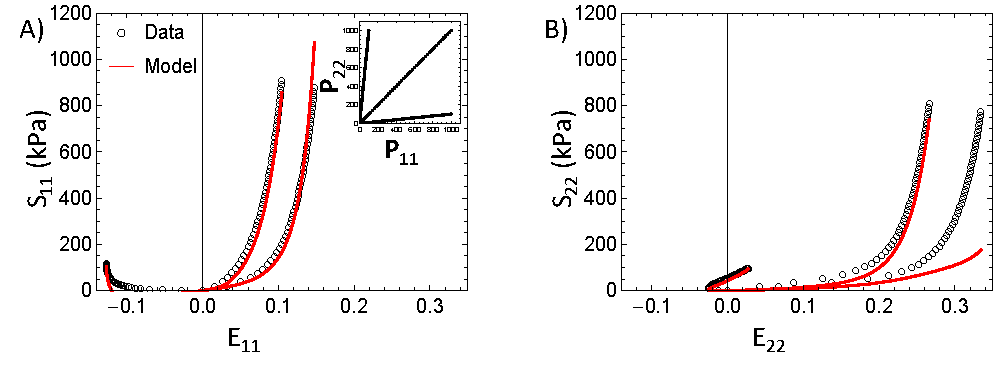
\includegraphics[width=\textwidth]{Images/chapter5/effphypred}
\caption{$\Psi_{eff}$ predicts the A) $S_{11}$ component and B) $S_{22}$ component of the unfitted loading paths very poorly even though the fit to the prestrained range is very good (Fig. \ref{fig:effphyfit}). The inset in A shows the corresponding loading paths.}
\label{fig:effphypred}
\end{figure} 
%-------------------	 end FIGURE 	-------------------%
%%%%%%%%%%%%%%%%%%%%%%%%%%%%%%%%%%%%%%%%%%%%%%%%%%%%%%%%%%%%


	

%%%%%%%%%%%%%%%%%%%%%%%%%%%%%%%%%%%%%%%%%%%%%%%%%%%%%%%%%%%%
%-------------------	begin FIGURE 	-------------------%
\begin{figure}[hptb]
\centering
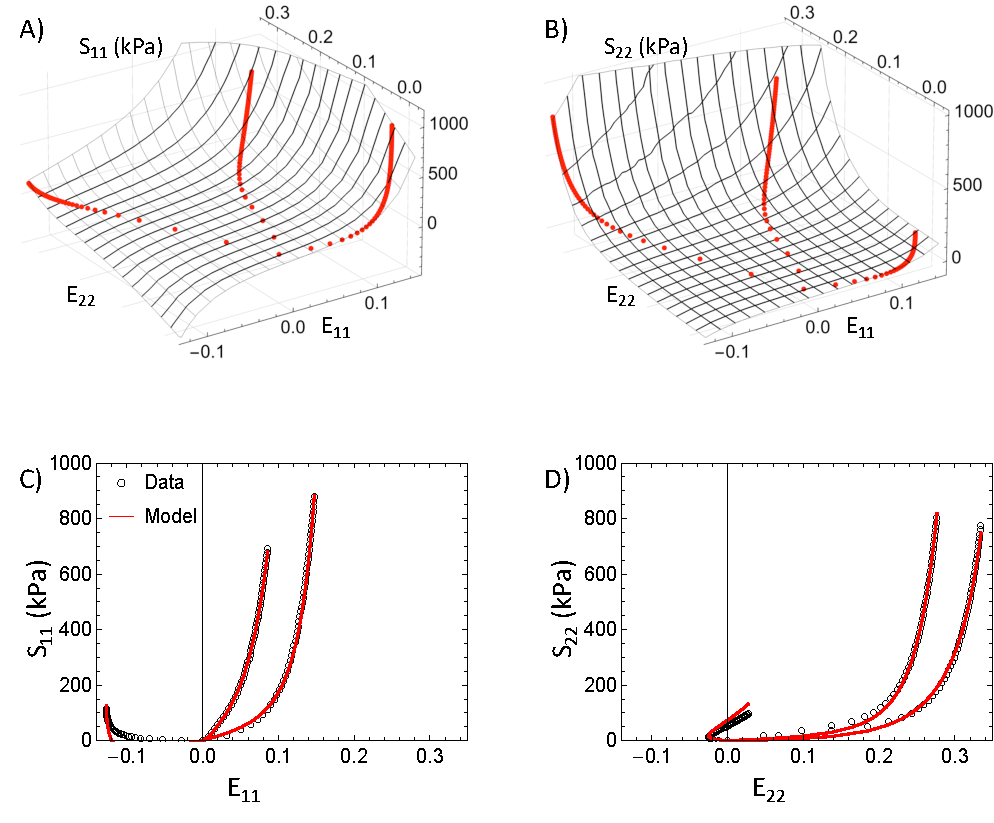
\includegraphics[width=\textwidth]{Images/chapter5/effoptfit}
\caption{$\Psi_{eff}$ fit optimal loading paths very well. A) The $S_{11}$ surface fitted to the data points. B) The $S_{22}$ surface fitted to the data points. C) Best fit of the $S_{11}$ component of the loading paths. D) Best fit of the $S_{22}$ component of the loading paths.}
\label{fig:effoptfit}
\end{figure} 
%-------------------	 end FIGURE 	-------------------%
%%%%%%%%%%%%%%%%%%%%%%%%%%%%%%%%%%%%%%%%%%%%%%%%%%%%%%%%%%%%

%%%%%%%%%%%%%%%%%%%%%%%%%%%%%%%%%%%%%%%%%%%%%%%%%%%%%%%%%%%%
%-------------------	begin FIGURE 	-------------------%
\begin{figure}[hptb]
\centering
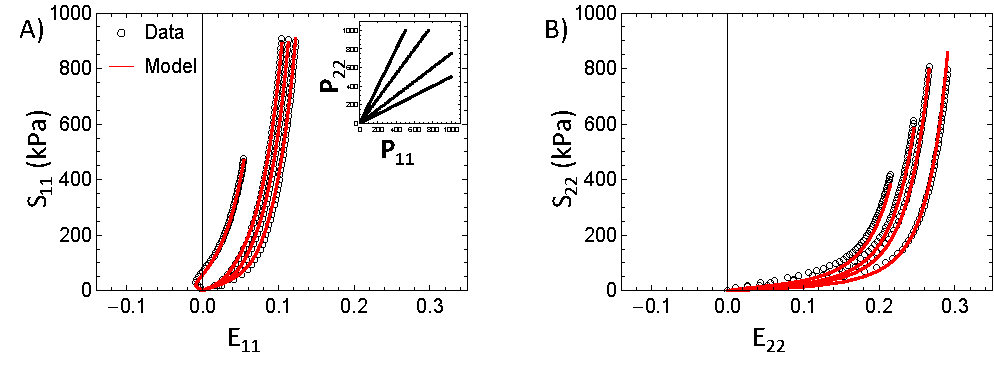
\includegraphics[width=\textwidth]{Images/chapter5/effoptpred}
\caption{Combining $\Psi_{eff}$ with optimal loading paths to predicts the A) $S_{11}$ component and B) $S_{22}$ component of the remaining unfitted loading paths very well from fit (Fig. \ref{fig:effoptfit}). The inset in B shows the corresponding loading predicted paths.}
\label{fig:effoptpred}
\end{figure} 
%-------------------	 end FIGURE 	-------------------%
%%%%%%%%%%%%%%%%%%%%%%%%%%%%%%%%%%%%%%%%%%%%%%%%%%%%%%%%%%%%





	



%%%%%%%%%%%%%%%%%%%%%%%%%%%%%%%%%%%%%%%%%%%%%%%%%%%%%%%%%%%%%
%%  Application to numerical simulations of BHVs under      %
%   quasistatic loading                                     %

\subsection{Numerical simulation of equibiaxial tension process and simulated bioprosthetic heart valve deformation}
	
    Planar biaxial test simulations were conducted to ensure that $\Psi_{eff}$ (Eqn. \ref{eqn:finalexponentialmodelformscaled}) and the elasticity tensor (Appendix \ref{sec:elasticitytensor}, Eqn. \ref{eqn:greenelasticityform}) were properly implemented in the finite element simulation framework.  We compared the computation time for both $\Psi_{eff}$ and Holzapfel-Gasser-Ogden model for biaxial simulation of bioprosthetic heart valve tissues and expectedly found no significant increase in computational cost. The total elapsed time for $\Psi_{eff}$ is 7.58 seconds in comparison to 6.40 seconds for the Holzapfel-Gasser-Ogden model, much faster than any micro-models can achieve.  

	Next we simulated tri-leaflet valves with model parameters derived from bovine pericardium, porcine aortic valve leaflet, and an idealized isotropic case. This is a simple demonstration of the use of the $\Psi_{eff}$ for the upscaling and homogenizing of micro-models. The model parameters for the bovine pericardium case were derived from the simplified structural model and model parameter of Aggarwal and Sacks \cite{aggarwal_inverse_2015}, and the resulting response matched very well qualitatively. Due to a lack of fiber mapping in the quasi-static simulation software used, some minor difference are still expected. We found no difficulty when simulating the pericardium, aortic, or isotropic valves. Suggesting that $\Psi_{eff}$ is quite robust numerically.
	
	
\begin{figure}
\centering
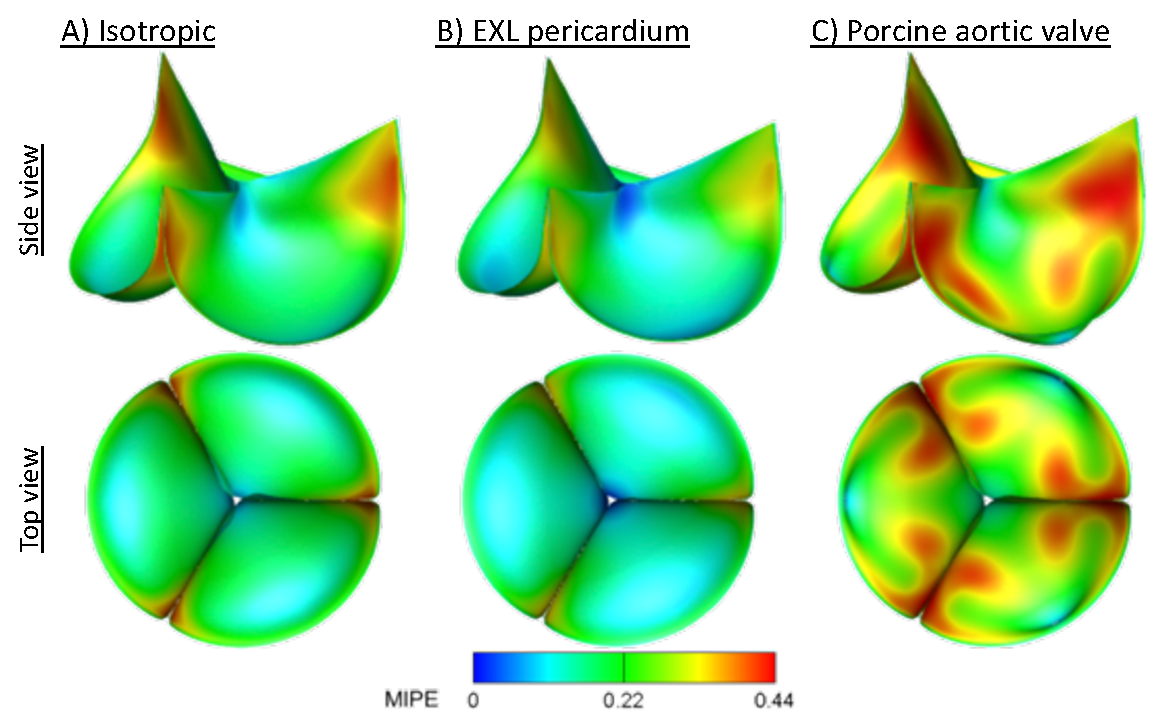
\includegraphics[width=\textwidth]{Images/chapter5/valvesimulations}
\caption{Simulations of intact tri-leaflet valves using A) the porcine aortic valve properties with an uniform fiber orientation distribution, B) exogenously cross-linked bovine pericardium properties with the most homogenous stress distribution, and C) the porcine aortic valve properties properties which results in a very heterogeneous stress distribution and the belly region caving in. The top row shows the side view of the valves at 80 mmHg and the bottom row shows the top-down view of the valves at the same transvalvular pressure.}
\label{fig:valvesimulations}
\end{figure}
    
    The material properties have significant effects on the mechanical behaviors of the leaflets (Fig. \ref{fig:valvesimulations}). The strain distributions within the leaflets were obtained for the pressure-loaded, fully-closed configurations of the valve, and then plotted with the maximum in plane Green-Lagrange strain (MIPE). When comparing the three different material, we can see that the native aortic valve properties result in significant heterogeneities in the deformation of the leaflets (Fig. \ref{fig:valvesimulations}C). Specifically, the belly region of the leaflets significantly protrudes out, increasing the load in the surrounding regions, especially near the commissures. This results in some stress concentrations that are not conducive to heart valve durability and health in general. The bovine pericardium valve (Fig. \ref{fig:valvesimulations}B) and the isotropic valve (Fig. \ref{fig:valvesimulations}A) on the other hand have significantly more homogeneous leaflet deformations, especially from the top-down view. Both of these undergo approximately the same deformation of 0.2 in MIPE. The largest difference between the two is near the commissure regions of the valve. Where the isotropic case is under significantly higher strain. Functionally, the material properties of the exogenously cross-linked bovine pericardium are the most suitable for heart valve leaflets, which distributes the stresses more evenly. 
    
    Much of the reasons behind these differences are likely to be due to the differences between the apparent mechanical properties \textit{in vivo} and the measured mechanical response in the laboratory setting. This is especially true for the aortic valve, which is extremely anisotropic with very high compliance in the radial direction of the leaflets. This difference is most likely due to the mismatch of referential configuration between the two states. Residual strain or residual stress has significant impact on the functional properties of the leaflets, specifically the apparent anisotropy and stiffness. Collagen fiber directions and varying regional properties can also have significant impact on the functional properties of the leaflets, and thus the results of the simulation. The valve leaflet shape, root geometry and properties, the arterial or ventricular geometry and loading conditions, can all be significant factors affecting the functions and stress distribution of the valve leaflets. Furthermore, how these factors affect the fluid dynamics of the valves is also an interesting question, suitable for further study. All in all, this is meant to be a demonstration and proof of concept for using $\Psi_{eff}$ to handle a wide range of soft tissue behaviors and anisotropy for the simulation of biological organs, in this case heart valves. Further and more detailed studies will be reserved for the future.  
  

    
    



%---    Discussion
%%%%%%%%%%%%%%%%%%%%%%%%%%%%%%%%%%%%%%%%%%%%%%%%%%%%%%%%%%%%%
%%	Discussion												%
%%%%%%%%%%%%%%%%%%%%%%%%%%%%%%%%%%%%%%%%%%%%%%%%%%%%%%%%%%%%%

\section{Discussion}

%-----------------------------------------------------------
%	Model performance
%-----------------------------------------------------------
\subsection{Using the effective constitutive model for homogenization in numerical simulations}

	The most fundamental issue with using phenomenological models for soft tissue and organ numerical simulations are that they 1) cannot simulate deformation beyond the range of data used for parameter estimation, and 2) cannot be widely used for tissues other than the ones they are specifically formulated for. Without being able to fully reproduce the response of micro-models, the resulting response may become inconsistent with the mechanisms of these micro-models, impacting their ability to simulate soft tissue responses, particular when modeling time-dependent processes. In the present work we found that using $\Psi_{eff}$ (Eqn. \ref{eqn:finalexponentialmodelformscaled}) along with optimally selected loading paths reconciles this issue. $\Psi_{eff}$ demonstrates much better capabilities at fitting the mechanical response of soft tissues in general. Admittedly, this may not be especially important for simulations of soft tissues in the normal physiological range as most models can fit the response of tissues if the range of deformation is small, as demonstrated with the generalized Fung model. However, for simulating abnormal conditions such as those that will drastically alters the deformation of the tissue, then using $\Psi_{eff}$ will be much more accurate. 
    
    
    The second and equally important part is the need for optimal data to determine the model parameters. Admittedly, the amount of data needed is not necessarily extensive. For example, we have shown that just three carefully selected loading paths can greatly improve the predictive capability of $\Psi_{eff}$ over the entire range of deformations. However, when the loading paths are selected poorly, $\Psi_{eff}$ still has some issue when predicting protocol beyond the range used to fit the model. Examples of this are when only using a single protocol under equi-biaxial stress (Appendix \ref{sec:otherresults}, Fig. \ref{fig:effequifit}D), or only using protocols in the prestrained range (Fig. \ref{fig:effphypred}). Mechanisms are still the major factor limiting the predictive capability in these cases. However, the intended role of $\Psi_{eff}$ is only to homogenize the response of mechanisms-based micro-models, not to help to better understand soft tissue function. The loading paths can be simulated by choice, thus should not be a major factor affecting $\Psi_{eff}$ in numerical simulations. 
    
    
    As we have shown, $\Psi_{eff}$ is able to handle a wide range of soft tissue behavior with no change in model form. This greatly simplifies the need of implementing a different constitutive models for every tissue type, especially when the Jacobian or the elasticity tensor must be implemented separately for computational efficiency, which can be quite complex, i.e. in ABAQUS UMAT. $\Psi_{eff}$ alone is capable of fully reproducing their mechanical response for simulations without significant loss in accuracy. Thus, the use of effective constitutive models can greatly facilitate in not only the computation speed of numerical simulations, but also the speed of implementing constitutive models of different soft tissue for simulations. In these cases, only the parameters of $\Psi_{eff}$ and organ geometry needs to be changed, as we demonstrated for the simulaiton of bovine pericardiu, porcine aortic and isotropic heart valves. $\Psi_{eff}$ is smooth, easily differentiable, and easy to implement. With optimal loading path and model scaling, the process of converting micro-model response to $\Psi_{eff}$ (Eqn. \ref{eqn:finalexponentialmodelformscaled}) should take not more than a few seconds, while saving a significant amount of time during numerical simulations. 
    
    
    On the other hand, micro-models are very useful for reproducing the response of tissue to which the full microstructure are known. This avoids the need for extensive mechanical data and parameter estimation, saving a time consuming step for evaluating different material designs. Some structural and geometry information may also be measurable \textit{in vivo} due to advances in techniques such as 3D ultrasound \cite{steiner_diagnostic_1994, yang_3d_2008, fenster_3_1996} and DT-MRI \cite{basser_vivo_2000, basser_microstructural_2011}, and can be directly incorporated into meso-scale structural models. However, these techniques are not yet sufficient to determine the mechanical properties of tissues. As such, micro-models are still a necessary and important part of any predictive simulation. Not surprisingly, even most traditional invariant based models, such as the Holzapfel-Gasser-Ogden model \cite{holzapfel_new_2000}, are being extended to incorporate the microstructures of the tissue \cite{holzapfel_modelling_2015}. 
    
    

%-------	growth and remodeling	-------%
\subsection{Effective constitutive model applications}

    One application of effective constitutive models is for simulating time-dependent processes, such as growth and remodeling. Growth and remodeling have been a long-time interest of the biomechanics community, and has important role in predictive simulations. Theories for growth and remodeling have been well studied, from Rodriguez in 1994 to Lanir and others in the current time \cite{lanir_mechanistic_2014, gleason_mixture_2004, rodriguez_stress_1994, humphrey_constrained_2002, cowin_tissue_2004, taber_biomechanics_1995}. The general theories for growth and remodeling involve the mechanisms for the changes in the reference configurations and a constrained mixture model involving the combined response of old original materials and new generated materials. This again multiplies the computational cost of the material models and the summation of many individual responses can significantly reduce numerical precision. Here homogenization using $\Psi_{eff}$ (Eqn. \ref{eqn:finalexponentialmodelformscaled}) can be useful. 
    

%-------	inverse modeling	-------%
    Another important application is for inverse modeling, which is important for patient specific modeling. Outside of \textit{in vitro} studies, performing the experiments necessary to determine the mechanical response of soft tissues is extremely difficult. Here, inverse modeling approaches are a solution to this problem \cite{lee_inverse_2014, aggarwal_inverse_2015, aggarwal_patient_2013, kim_inverse_2009, liu_inverse_2013}. In inverse modeling, the model parameters and the errors between the simulated and measured strains are simultaneously optimized. However, the available data that can be obtained \textit{in vivo} is limited, and is not always sufficient to accurately determine the model parameters. In these cases, the tissue microstructure can be used along with meso- and multi-scale models to narrow down the range of possible parameters. However, this multiplies the already hefty costs of the these constitutive models. Here, the approach we proposed (Fig. \ref{fig:simulationframework}B) can be used to reduce computational cost.

 


%-----------------------------------------------------------
%	Model scaling method
%-----------------------------------------------------------

\subsection{Model scaling method in other applications}
    
    Although not introduced as such, the model scaling method, or a similar technique to this, was briefly described by Fung \textit{et al.} in their original work on the mathematical modeling of arteries \cite{fung_pseudoelasticity_1979}. The paper introduced the strain energy density function as 
%==========================================================%
%-------------------	begin EQUATION 	-------------------%
\begin{equation}\label{eqn:fungarterymodel}
\rho_0 W^{(2)} = \frac{C^\prime}{2}\operatorname{exp}\left[\alpha_1 \left(E_{\theta\theta}^2 - E_{\theta\theta}^{*2} \right) + \alpha_2 \left(E_{zz}^2 - E_{zz}^{*2} \right) + \alpha_4 \left(E_{\theta\theta}E_{zz} - E_{\theta\theta}^*E_{zz}^* \right) \right]
\end{equation}
%-------------------	 end EQUATION 	-------------------%
%==========================================================%    
    in equation 2 of the said work ($C$ is changed to $C^\prime$ to consistency in notation with the present work). $E_{\theta\theta}^*$ and $E_{zz}^*$ are introduced as strains corresponding to some fixed stresses of $S_{\theta\theta}^*$ and $S_{zz}^*$, usually taken in the physiologic range. Similarly, this "scaling" can be absorbed into the parameter $C^\prime$ like in the present work. This idea was not greatly expanded upon, but \textit{Fung et al.} notes that:
\begin{quotation}
"But in practice it is very helpful to introduce $E_{\theta\theta}^*$ and $E_{zz}^*$. Not only are the values corresponding to $S_{\theta\theta}^*$ and $S_{zz}^*$ very important information, but also their use makes the constants [$C^\prime$], $\alpha_1$, $\alpha_2$, and $\alpha_4$ much more stable for each set of specimen." \cite{fung_pseudoelasticity_1979}
\end{quotation} 
    and that 
\begin{quotation}
"[$E_{\theta\theta}^*$ and $E_{zz}^*$] are indexes of compliance of the vessel. Using $E_{\theta\theta}^*$ and $E_{zz}^*$, the variations of the constants $C$, $\alpha_1$, $\alpha_2$, and $\alpha_4$, which determines the shape of the stress-strain curve, are greatly reduced. The assignment of $S_{\theta\theta}^*$ and $S_{zz}^*$ is arbitrary, but hopefully standard values will be adopted by the biomechanics community." \cite{fung_pseudoelasticity_1979}
\end{quotation}

	In truth, we did not find that the model scaling method necessarily makes $\alpha_1$, $\alpha_2$, and $\alpha_4$ more consistent, but rather that they are exactly the same values with or without this method, assuming parameter estimation was not trapped in some local minimum. The model scaling method does make reaching the values of these parameter more consistent. The biggest benefit remains the significant improvement in the correlation between the parameters $C^\prime$ and $\alpha_1$, $\alpha_2$, and $\alpha_4$, improving the conditioning of the objective function surface during parameter estimation. It also imparts some physical meaning to the value of $C^\prime$, or for $A_s$ and $c_0^\prime$ in present work. For Fung \textit{et al.}, this is some arbitrary physiologic stresses, for us, this is exactly 'maximum' (with respect to the objective function) value of strain energy within the data used for parameter estimation. This does bestow some consistency to the value of $C^\prime$, as it is exactly the total strain energy density at the stresses of $S_{\theta\theta}^*$ and $S_{zz}^*$, which will likely be similar between specimens taken from the same arteries from health subjects. However, the choice of $E_{\theta\theta}^*$ and $E_{zz}^*$, or $E_m^\mathrm{max}$, $E_n^\mathrm{max}$, and $E_\phi^\mathrm{max}$ for $\Psi_{eff}$ (Eqn. \ref{eqn:finalexponentialmodelformscaled}), should not be arbitrary. The model scaling method works due to altering the functional effect of $c_0$ and $b_i$, or $C$ and $\alpha$. $E_m^\mathrm{max}$, $E_n^\mathrm{max}$, and $E_\phi^\mathrm{max}$ should be chosen deliberately so that area under the constitutive model, based on the objective function, remains approximately the same, thus decoupling changes in modulus and changes in curvature from the exponential parameters. 


	Perhaps, the biggest advantage of the model scaling method is that it is applicable to nearly any constitutive model with an exponential function, such as models like the Holzapfel-Gasser-Ogden, Humphrey, Vito, or even the meso-scale structural model with simplified ensemble response such as in Fan and Sacks \cite{fan_simulation_2014a}, Lee \textit{et al.}\cite{lee_effects_2015}, and Aggarwal and Sacks \cite{aggarwal_inverse_2015}. Even polynomial model forms with a power law, $\Psi=A\epsilon^B$, such as the generalized Ogden model, or the elastin model for the mitral valve in Zhang et al. \cite{zhang_meso_2016} can see benefits from the model scaling method. In this case, the scaling term becomes $A = \bar{A} e^{-B \log(\epsilon_{max})}$. In summary, this model scaling method should have significantly implications in improving the speed and consistency of parameter estimation for any model with an exponential like form.
    
    
    
    
%-----------------------------------------------------------
%	Optimal
%-----------------------------------------------------------	
\subsection{The equibiaxial stress protocol in optimal loading paths}

    One highlight from the optimal loading path study is that the equibiaxial stress loading path is extremely important. The equibiaxial stress loading path is always the one shown in figures for most paper, as it gives most intuitively understandable information on the mechanical properties of the tissue. It gives insights into the general form, anisotropy and stiffness of the material at a glance, and is not surprisingly also the best loading path for parameter estimation. However, it is surprising just how little the equibiaxial stress loading path can provide alone. The difference in magnitude between the D-optimality values for one vs. two loading paths is almost 20. The equibiaxial stress alone simply is not enough to determine the material parameters using phenomenological approaches. However, with the addition of one or two more protocols, even if they are along a similar loading paths can significantly improve the predictive capabilities. However, this may be partially overcome by meso-scale structural approaches, given the information on the microstructure of the tissue.


\subsection{Alternative options for optimal \textit{in silico} loading paths}

	The limitation on predicting outside of the loading paths used for parameter estimation can be somewhat remedied by densely sampling the response of the micro-model over a larger range of deformations. However, this is not entirely ideal for computational speed during parameter estimation, and choosing the sampling points for parameter estimation is not a trivial task itself. Points with high stresses tend to weight heavily during parameter estimation, proper care needs to be taken to capture both the high stress and low stress response. Given that the number of data points scales cubically with the distance between data points, this approach is still limited. 

    
    Having said this, our investigation of optimal loading paths is restricted to constant strain ratios or constant stress ratios. In reality, there are many ways to define loading paths, some can be quite creative. We do not deny the possibility of other forms of loading paths that are more optimal. However, the current approach with three, or at most five protocols, is already sufficient. We did test some alternative loading paths, such as Fung \textit{et al.}'s post pre-strain loading paths \cite{fung_pseudoelasticity_1979}. They cover much of the physiological range, but are still insufficient for parameter estimation. Increasing the number of loading paths in this case has minor improvements, but pales in comparison to just picking better types of loading paths. The poor predictive capabilities for the low stress region can have significant impacts on underestimating the mechanical properties of matrix and elastin, and their properties can be important to the functions of micro-models. The mechanical properties of the matrix for example, having significant implications for simulating the process of permanent set in exogenously cross-linked soft tissues \cite{zhang_modeling_2017}. Failing to properly reproduce this response, can affect the predictive capabilities of the associated micro-models, causing the whole framework of using $\Psi_{eff}$ to facilitate numerical simulations (Fig. \ref{fig:simulationframework}B) to fall apart. 
    
    










%---    Conclusion
%%%%%%%%%%%%%%%%%%%%%%%%%%%%%%%%%%%%%%%%%%%%%%%%%%%%%%%%%%%%%
%%	Conclusion												%
%%%%%%%%%%%%%%%%%%%%%%%%%%%%%%%%%%%%%%%%%%%%%%%%%%%%%%%%%%%%%

% \section{Limitations and conclusion}

%-----------------------------------------------------------
%	Limitations
%-----------------------------------------------------------
\section{Limitations} 
	
    One major limitation of $\Psi_{eff}$ (Eqn. \ref{eqn:finalexponentialmodelformscaled}) is the large number of parameters, 14 in the fully generalized form. This is not very favorable, as the time complexity for most optimization algorithms scales nonlinearly with the number of parameters. However, $\Psi_{eff}$ has very low computational cost, and reasonably low parameter covariance, thus this should not be a major problem. Alternatives are also less favorable, as they either require more parameters or cannot sufficiently capture the response of soft tissues in a wide range or reproduce the response of multiple tissue types. 
    
    Another limitation, which also applies to all phenomenological models, is that $\Psi_{eff}$ has no intrinsic mechanisms built in. Without sufficient mechanical data to derive the model parameters, phenomenological models have limited predictive capabilities. Specifically, the phenomenological models perform poorly when extrapolating outside of the range of available data. This also means that phenomenological models can only provide limited information on how the tissue functions. It can reproduce the mechanical response of soft tissues very well, but it is also harder to infer more about the structure and function of the tissue. This is not a major concern for us. For the mechanisms or the structure to function relationship of soft tissues, micro-models already fulfills the need. $\Psi_{eff}$ is intended as a fit all model for fulfilling the gap between predictive micro-models and computationally efficient simulations. With carefully selected of loading paths for parameter estimation (Section \ref{sec:optimaldesign}), $\Psi_{eff}$ can accurately reproduce the mechanical response of soft tissue within the expected range. In other words, $\Psi_{eff}$ does not have to be able to predict the mechanical response of soft tissues under unmeasured and extrapolated deformations, it only has to be able to fully reproduce the entire range of responses predicted by the micro-models, which is its main purpose. 



%-----------------------------------------------------------
%	Conclusion
%-----------------------------------------------------------
\section{Conclusion and Future Directions} 

	In this work, we developed a constitutive model form for the effective response of planar soft tissues. This effective constitutive model (Eqn. \ref{eqn:finalexponentialmodelformscaled}) is applicable to a wide range of soft tissue responses, while being as computationally efficient as most common phenomenological approaches, such as Holzapfel-Gasser-Ogden or the generalized Fung model. This model utilizes the modeling scaling method for minimizing covariance between parameter, which shows significant improvements in the speed and accuracy of parameter estimation. We have shown that our effective constitutive model along with optimal loading paths is able to fully replicate the response of complex meso-scale structural models for the entire range of deformations, whereas most phenomenological models have difficulties when predicting unfitted loading paths. The effective constitutive model is robust enough to be able to handle a wide range of soft tissue behaviors and anisotropy for accurate numerical simulations, such as in simulations of heart valves. Thus, the effective constitutive model can play an important role for the upscaling and homogenization of the response of complex micro-models for improving the efficiency of organ-level simulations. 
    

	One nature extension to this effective modeling approach is for 3 dimensional soft tissues. The extension to 3 dimensions doubles the number of inputs in comparison to planar models, with the additional inputs being $E_{13}$, $E_{23}$, and $E_{33}$. This means that the initial most generalized form for the 3-D soft tissue models (Eqn. \ref{eqn:exponentialmodelform}) has 209 terms before reduction. This is unmanageable for establishing the initial approach, where using a planar soft tissue model is more suitable. However, applying the same restrictions to the model form (section \ref{sec:finalform}) reduces this to 48 terms. This is possible due to symmetry by expressing the components of the Green-Lagrange strain tensor with respect to the material axis (Eqn. \ref{eqn:greenstrain}). This is not so easy to do in 3-dimensions, requiring a third vector corresponding to the direction of least stiffness, which in turn requires the 3 dimensional fiber orientation distribution. 
    
    
    
    
    
    
    
    





%---    Bioliography
\bibliographystyle{plainnat}
\bibliography{phd}

\chapter{Numerical simulation of intact bioprosthetic heart valves}

\section{The changes in the response of bioprosthetic heart valves to cyclic loading}
\subsection{Accelerate wear testing bioprosthetic heart valves}
\subsection{Design of study}

\section{Frame work for time evolving simulation}

\section{Simulating the effect of accelerated wear testing on bioprosthetic heart valves*}

Final paper

\chapter{Conclusions, and future directions}

\section{Summary}
    
    Soft-tissue-derived exogenously cross-linked (EXL) biomaterials continue to play an important role in the fabrications of bioprosthetic heart valves (BHV), by having advantages in immunogenic and mechanical behaviors \cite{starr_artificial_2007}. Despite ongoing research, our understanding of these materials and of the mechanisms leading to their failure remains at an empirical level. A significant challenge prohibiting accurate and predictive simulations of BHVs is a lack of understanding of the mechanism of BHV failure. One significant mechanical change in response to cyclic loading is the change in geometry of the BHV leaflets. This process is induced by permanent set, which changes the referential configuration of the leaflet material and thus how they deform in response to transvalvular loading. The further analysis has shown that significant structural damage occurred within the same region that undergoes significantly permanent set \cite{smith_fatigue_1999}. Permanent set occurs only within the early stages after surgical implantation. Although no structural damage occurs, this has important implications in geometrical change and durability of BHVs. Using permanent set we can predict change in geometry and optimal the initial design of BHVs for increase durability. To develop the constitutive model and framework for numerical simulation, we have taken the following steps:
    
    \begin{enumerate}
        \item We developed a meso-scale structural constitutive model for soft tissues. Constitutive models are fundamental to developing a deeper understanding of and predicting soft tissue function and pathology. To develop this constitutive model, we utilized the MV leaflets as an example. This model takes into account the layered structure of these tissues and the contributions from the distinct collagen and elastin fiber networks within each tissue layer. The requisite collagen and elastin fibrous structural information for each layer was quantified using second harmonic generation microscopy and conventional histology. A comprehensive mechanical data set was also used to guide the model formulation and parameter estimation. Furthermore, novel to tissue-level structural constitutive modeling approaches, we allowed the collagen fiber recruitment function to vary with orientation. Finally, a novel fibril-level (0.1 to 1 $\mu$m) validation approach was used to compare the predicted collagen fiber/fibril mechanical behavior with extant MV small angle X-ray scattering data. Results demonstrated excellent agreement, indicating that the MSSCM fully captures the tissue-level function. Future utilization of the MSSCM in computational models of the MV will aid in producing highly accurate simulations in non-physiological loading states that can occur in repair situations, as well as guide the form of simplified models for real-time simulation tools.
        \item We extended the meso-scale structural modeling approach for the effect of exogenous crosslinking, which is a crucial part of the fabrication of BHVs to suppress immunogenicity. Despite decades of research, development and clinical use, no such model previously existed. In this study, we develop the first rigorous full structural model (i.e. explicitly incorporating various features of the collagen fiber architecture) for exogenously cross-linked soft tissues. This was made possible, in part, with the use of native to cross-linked matched experimental data sets and an extension to the collagenous structural constitutive model so that the uncross-linked collagen fiber responses could be mapped to the cross-linked configuration. This allowed us to separate the effects of cross-linking from kinematic changes induced in the cross-linking process, which in turn allowed the non-fibrous tissue matrix component and the interaction effects to be identified.  The most novel findings of this study were that: (i) the effective collagen fiber modulus was unaffected by cross-linking and (ii) fiber-ensemble interactions played a large role in stress development, often dominating the total tissue response (depending on the stress component and loading path considered).
        \item We extended this constitutive model further for time-dependent effects like permanent set. Permanent set is an effect which causes BHVs to undergo significant changes in geometry with in vivo operation, which leads to stress concentrations that can have a significant impact on structural damage. These changes do not appear to be due to plastic deformation, as the leaflets only deform in the elastic regime. Moreover, structural damage was not detected by the 65 million cycle time point. We hypothesize that the scission-healing reaction of glutaraldehyde is the underlying mechanism responsible for permanent set in exogenously crosslinked soft tissues. The continuous scission-healing process of glutaraldehyde allows a portion of the exogenously crosslinked matrix, which is considered to be the non-fibrous part of the extracellular matrix, to be re-crosslinked in the loaded state. To model the permanent set effect, we assume that the exogenously crosslinked matrix undergoes changes in reference configurations over time. The changes in the collagen fiber architecture due to dimensional changes allow us to predict subsequent changes in mechanical response. Results show that permanent set alone can explain and, more importantly, predict how the mechanical response of the biomaterial change with time. An important finding we have is that the collagen fiber architecture has a limiting effect on the maximum changes in geometry that the permanent set effect can induce. This is due to the recruitment of collagen fibers as the changes in geometry due to permanent set increase. This means we can potentially optimize the BHV geometry based on the predicted the final BHV geometry after permanent set has largely ceased. 
        \item We developed a framework for the use of effective constitutive models to homogenize and facilitate numerical simulations. Effective which only reproduces the essential responses of soft tissue but not the underlying mechanisms. Current soft tissue constitutive modeling approaches have become increasingly complex, often utilizing meso- and multi-scale methods for greater predictive capability and linking to the underlying mechanisms. However, such modeling approaches are associated with substantial computational costs, making the use of effective constitutive model approaches an important part of efficient numerical simulations. We evaluated this approach and demonstrated that it is able to handle materials of widely varying degrees of anisotropy, such as exogenously cross-linked bovine pericardium and aortic valve leaflet. This effective constitutive model approach has shown significant potential for improving the computational efficiency and numerical robustness of multi-scale and meso-scale modeling approaches, facilitating the application of inverse modeling and simulations of growth and remodeling of soft tissues and organs.
        \item Finally, we completed this process by developing a Python-based framework for the implementation and simulation of permanent set. This simulation utilizes the predictive mechanism based constitutive model for the permanent set effect in exogenously crosslinked soft tissues that we previously developed. We have shown that we can use this simulation to predict the evolving geometry, microstructural and material property changes. These results can then be used to predict regions of increasing likelihood of structural damage and can be used to optimize the initial design of BHVs based on these factors. Most important of these effects is that the collagen fiber architecture can play a role in limiting the permanent set effect, where the straightening of collagen fibers prevents further changes in geometry. Thus, accounting for the permanent set effect is especially important in the design of BHVs to better improve their performance and durability. 
    \end{enumerate}
    
\section{Conclusions}

    In conclusion, we have developed a novel predictive and mechanism-based constitutive modeling and numerical simulation framework for the time-dependent simulation of bioprosthetic heart valves. This work has important implication for predicting BHV durability. By being able to predict the evolving geometry of BHVs, we can utilize this approach for optimizing the initial design of BHVs for more homogeneous distributed loading to the constitutive collagen fibers as well as better fluid dynamics. With future extensions to this model and framework, this can open the door to improving the process for BHV design and thus more durable BHVs. 


    
\section{Future directions}
    
    The next sequential step for this work is the inclusion of structural damage to the constitutive model. Part of the reason preventing the inclusion of structural damage to this current work is the lack of sufficient experimental data. Structural damage is difficult to quantify as it only gradually accumulates over long periods of time. Due to the exponential nature and large structural reserves of soft tissues, small decreases in the number or modulus of collagen fiber is very difficult to detect. This is also complicated by the fact that strain is difficult to quantify in the first place. In accelerated wear testing or other similar environments, this process is further complicated by the heterogeneity of the resulting response. However, by simulation and removing of the permanent set effect on the change in geometry, we can more accurately determine the remaining changes due to structural damage. This opens the doors to the development of mechanism-based structural damage models which is lacking in literature. 
    
    
    Another part of this ongoing project is the simulation of the fluid dynamics of the BHVs in response to the complex environment surrounding tissues. Fluid-solid interactions (FSI) have long been a popular field of study \cite{kamensky_immersogeometric_2015}\cite{hsu_dynamic_2015}\cite{wu_anisotropic_2018}\cite{kiendl_isogeometric_2015}. However, this permanent set framework opens the doors to evaluating how the fluid dynamics change over time in response to cyclic loading. The FSI finite element soft is directive included in the permanent set simulations to facilitate this extension, and more parametric studies to evaluated and optimize BHV design designs. This also lends itself to help us better understand the results of accelerated wear testing environments, which as FDA required but drastically differs from the in vivo environments. This will provide a better analysis of fatigue testing results, better prepare these designs for clinical trials and surgical implantation. 
    
    
    Growth and remodeling is a similar important future area, as this has important implications in the prediction of the outcomes of diseases, injuries, and surgical interventions. The permanent set model and simulation framework developed herein is a simplification of the growth and remodeling framework by removing the growth component. This can have important potential implications are devices such as tissue engineered valves which have the possibility of growing and adaption to the surrounding environment if seeded with interstitial cells. In addition to the exogenously crosslinked tissue applications addressed herein, we have observed permanent set like phenomenon in mitral valve tissue during pregnancy \cite{rego_mitral_2016}. In that study, our results suggested that much of the growth and remodeling in the MV leaflet does not begin immediately, but rather undergoes mostly passive leaflet enlargement until these parameters reach a critically low level, at which point growth and remodeling are triggered. This initial tissue distension process is very similar in behavior to the permanent set mechanism outlined in the present work. Thus, the current approach could be applied to the early phases of soft tissue remodeling, where non-failure mechanisms occur before the onset of growth of tissue growth and remodeling. This is the advantage for the structural-based approach to modeling permanent set, which allows us to describe the mechanical response based on real physically measure-able quantities. 
    

\newpage
%---    Bioliography
\bibliographystyle{plainnat}
\bibliography{phd}
    
 


\appendices

% \chapter{Improved method for the analysis planar biaxial mechanical data}

\section*{Preface}
\addcontentsline{toc}{section}{Preface}%

Simulation of the mechanical behavior of soft tissues is critical for many physiological and medical device applications. Accurate mechanical test data is crucial for both obtaining the form and robust parameter determination of the constitutive model. For incompressible soft tissues that are either membranes or thin sections, planar biaxial mechanical testing configurations can provide much information about the anisotropic stress–strain behavior. However, the analysis of soft biological tissue planar biaxial mechanical test data can be complicated by in-plane shear, tissue heterogeneities, and inelastic changes in specimen geometry that commonly occur during testing. These inelastic effects, without appropriate corrections, alter the stress-traction mapping and violates equilibrium so that the stress tensor is incorrectly determined. To overcome these problems, we presented an analytical method to determine the Cauchy stress tensor from the experimentally derived tractions for tethered testing configurations. We accounted for the measured testing geometry and compensate for run-time inelastic effects by enforcing equilibrium using small rigid body rotations. To evaluate the effectiveness of our method, we simulated complete planar biaxial test configurations that incorporated actual device mechanisms, specimen geometry, and heterogeneous tissue fibrous structure using a finite element (FE) model. We determined that our method corrected the errors in the equilibrium of momentum and correctly estimated the Cauchy stress tensor. We also noted that since stress is applied primarily over a subregion bounded by the tethers, an adjustment to the effective specimen dimensions is required to correct the magnitude of the stresses. Simulations of various tether placements demonstrated that typical tether placements used in the current experimental setups will produce accurate stress tensor estimates. Overall, our method provides an improved and relatively straightforward method of calculating the resulting stresses for planar biaxial experiments for tethered configurations, which is especially useful for specimens that undergo large shear and exhibit substantial inelastic effects.



%---    INTRODUCTION
\section{Introduction}
    A central need in the application of continuum mechanics to biological tissues is the development of the constitutive models. Such models are critical for insights into the development of accurate computational simulations of the heart and its valves, arteries, cartilaginous structures, and engineered tissue equivalents. While the formulation of the theoretical framework is always the first step, rigorous experimentation must be performed in parallel to explore all relevant deformations to both obtain the necessary constitutive model parameters and evaluate its predictive capabilities \cite{sacks_biaxial_2000}. Thus, there is an increasing need for multi-axial mechanical data to fully explore and understand the complex structures of biological tissues. For incompressible planar membrane or thin soft tissue sections, a planar biaxial mechanical testing configuration can provide much information about the stress–strain behavior \cite{sacks_biaxial_2000}. Planar biaxial tests can be performed with either extensional deformations only, or in combination with in-plane shear \cite{sun_biaxial_2003}.


    However, an ongoing problem in soft tissue mechanics is that they are not truly elastic. Soft tissues have been shown to exhibit elastic behavior under physiological conditions, yet also exhibit permanent setlike changes in configuration from preconditioning \cite{sacks_biaxial_2000}\cite{sun_biaxial_2003}\cite{stella_time_2007}. In addition, due to their very low stiffness in the zero stress state, even mounting and handling can alter the shape of the test specimen. This may result in a drastic change in the stress-free reference state of the specimen from the one measured prior to mounting. The situation becomes more complex when shear strains are involved. In our first studies \cite{sacks_method_1999}, a simplified method was used to determine the components of the first Piola–Kirchhoff stress tensor $P$ from the initial dimensions and experimentally measured axial forces, with the second Piola–Kirchhoff stress tensor $S$ determined using $S = F^{-1}P$. We later noted that this mapping did not produce fully accurate results in cases where the shear strain was substantial. An initial alternative method was developed \cite{freed_hypoelastic_2010}, but was not a generalized solution. Specifically, the method did not accounted for changes in geometry of the unloaded state as a result of preconditioning and other related inelastic dimensional effects. As a result, the run-time specimen configuration will be a quadrilateral due to both shear and extensional strains that occurred during preconditioning. While others have developed various methods of deriving the stress under biaxial testing (e.g. \cite{fomovsky_evolution_2010}), no method to date addresses the actual testing geometry or compensates for changes in specimen geometry during the experiment. Moreover, inherent heterogeneities in tissue structure will always affect the accuracy of the resultant stress analysis. No systematic study to date has incorporated these effects nor determined their influence on the accuracy of stress tensor components from planar biaxial tests.
    
    
    In approaching a solution to this problem, we first recognized certain key considerations and limitations inherent in interpreting any biaxial mechanical data. As noted in Sun et al. \cite{sun_numerical_2003}, no biaxial experimental configuration can produce an ideal homogeneous strain and stress state. This will result in subsequent errors in the computation of stress tensor components, which will propagate into the estimates of the material parameters, ultimately limiting our ability to accurately simulate soft tissues. Moreover, we believe one should first determine the constitutive model form and material parameters before undertaking the complex task of simulating complete organ systems. Thus, there remains a need for an improved method to derive the stress–strain relation directly from biaxial mechanical test data, with the assumption of homogeneous strain and stress fields.
    
    
    The current work presents a straightforward, generalized approach for computing the effective Cauchy stress tensor for planar biaxial mechanical experiments that utilize a tethered mounting configuration. This method utilizes only the (1) the initial specimen dimensions, (2) the measured fiducial markers positions, and (3) the measured axial forces. It works under the assumption of homogeneous strain and stress fields within the specimen and compensates for the following attributes:
        \begin{enumerate}
            \item changes from the unloaded, initially measured specimen geometry to the postmounted, preconditioning state
            \item the effects of structural heterogeneities in tissues, which can result in rigid body rotations
            \item actual specimen geometry and tether attachment configurations during run time
        \end{enumerate}
    To assist with validation and provide additional insights, we also present a comprehensive simulation of the entire biaxial testing geometry using simulated tissue properties, anisotropy, and structural heterogeneities.

%---    METHODS
\section{Methods}

\subsection{Kinematics of a Planar Biaxial Test}
    
    Assuming a homogenous deformation, the kinematical description of the planar biaxial test is
        %-------------------	begin EQUATION 	-------------------%
        \begin{equation}
        \begin{aligned}
        x_1 = \lambda_1X_1+\gamma_1X_2, \quad x_2 = \lambda_2X_2+\gamma_2X_1, \quad x_3 = \lambda_3X_3
        \end{aligned}\label{A:eqn:1}
        \end{equation}
        %-------------------	 end EQUATION 	-------------------%
    where $X_k$ and $x_k$ are coordinates for material particles in the reference and current configurations, respectively, $\lambda_k$ are the stretches and $\gamma_k$ are the shears. The shear relative to the third axis is 0, with resulting deformation gradient tensor $\mathbf{F}$
        %-------------------	begin EQUATION 	-------------------%
        \begin{equation}
        \begin{aligned}
        \mathbf{F} = 
        \begin{bmatrix}
        \dpd{x_1}{X_1} & \dpd{x_1}{X_2} & \dpd{x_1}{X_3} \\
        \dpd{x_2}{X_1} & \dpd{x_2}{X_2} & \dpd{x_2}{X_3} \\
        \dpd{x_3}{X_1} & \dpd{x_3}{X_2} & \dpd{x_3}{X_3}
        \end{bmatrix}
        = 
        \begin{bmatrix}
        \lambda_1   & \gamma_1  & 0 \\
        \gamma_2    & \lambda_2 & 0 \\
        0           & 0         & \frac{1}{\lambda_1\lambda_2 - \gamma_1\gamma_2}
        \end{bmatrix}
        \end{aligned}\label{A:eqn:2}
        \end{equation}
        %-------------------	 end EQUATION 	-------------------%
    Note that $F_{33} = (\lambda_1\lambda_2 - \gamma_1\gamma_2)^{-1}$ is computed by the incompressibility constraint $det(\mathbf{F}) = 1$. All specimen deformations are assumed to be completely quantified from the interior of the specimen (approximately the inner third by linear dimension or area) using fiducial markers or texture mapping techniques \cite{sacks_biaxial_2000}\cite{jor_estimating_2010}.
    
    
\subsection{Analysis of Stress}

\subsubsection{Planar Biaxial Testing Experimental Configuration}

    Planar biaxial devices follow a typical design overall, but vary in the specific boundary conditions utilized. We start with a rectangular specimen with known side lengths $L_1$ and $L_2$, and an initial thickness $L_3$, and then mounted with resultant forces $f^{(1)}$ and $f^{(2)}$ (Fig. (Fig.1).1). Previously, we determined the stresses using
        %-------------------	begin EQUATION 	-------------------%
        \begin{equation}
        \begin{gathered}
        P_{11} = \frac{f_1^{(1)}}{A^{(1)}}, \quad P_{22} = \frac{f_2^{(2)}}{A^{(2)}}, \quad P_{11} = P_{22} = 0 \\
        \mathbf{P}
        =   \begin{bmatrix}
            P_{11} & P_{12} \\
            P_{21} & P_{22} 
            \end{bmatrix}
        \end{gathered}\label{A:eqn:3}
        \end{equation}
        %-------------------	 end EQUATION 	-------------------%
    where $\mathbf{f^{(i)}}$ and $A^{(i)}$ are the axial forces and initial cross-sectional areas, respectively, with $i = {1,2}$ \cite{sacks_method_1999}. The Cauchy stress $\mathbf{t}$ and second Piola–Kirchhof stress tensor $\mathbf{S}$ are computed using standard formulations $\mathbf{t} = \mathbf{P} \cdot \mathbf{F}^\mathsf{T}$ and $\mathbf{S} = \mathbf{F}^{-1}\mathbf{P}$.
    
    
    It should be noted that the methods of attachment are generally separated into tethered \cite{sacks_biaxial_2000}\cite{bellini_biaxial_2011}\cite{azadani_comparison_2012}\cite{kamenskiy_passive_2014}\cite{gregory_comparison_2011} and clamped boundaries \cite{sun_effects_2005}\cite{oconnell_human_2011}\cite{sommer_multiaxial_2013}\cite{hu_influence_2013}\cite{simon-allue_unraveling_2014}. In the present work, we focus on tethered boundary configurations. We do not intend to convey that any particular method is optimal for any application, but rather to show that a tethered attachment system, with its ability to allow free lateral displacements and to apply relatively uniform distribution of boundary forces, can be used to accurately obtain the stress–strain relation directly from the experimentally obtained data. We feel this is important as the first step in any tissue mechanical analysis in order to establish the form of the strain energy function, which is best done using directly determined S and F whenever possible. As such, this method will only require direct measurement of (1) initial specimen dimensions, (2) fiducial marker positions, and (3) the measured axial forces. Due to the intrinsic differences in the stress state induced, this method will not be directly applicable to clamped boundaries. Additionally, the following assumptions are made throughout the present work:
        \begin{enumerate}
        \item The tissue is at all times in quasi-static equilibrium.
        \item The deformations are homogeneous, and consequentially:
            \begin{enumerate}
                \item The specimen is located at the center of the apparatus and does not translate.
                \item The testing system is symmetric.
            \end{enumerate}
        \item The applied tractions are evenly distributed per side, given by the average applied by the four attached tethers.
        \end{enumerate}
    
    
\subsubsection{Mounting and Preconditioning Effects}

    Distortions will occur to some extent during mounting and testing due to the high compliance of soft tissue specimen in the low stress range. Although the mechanisms for preconditioning effects remain unknown, it is known that the effect is not strictly viscoelastic \cite{sacks_biaxial_2000}\cite{lanir_structural_1979}\cite{lanir_two_1974}. Instead, it is similar to permanent-set like effects, but is reversible over time \cite{sacks_biaxial_2000}. For example, it has been shown that the process itself reverts over the course of 24 hrs in chemically treated pericardium tissue \cite{sacks_biaxial_2000}. Thus, the effect only lasts for the current test and is utilized to induce a stable, repeatable response \cite{sacks_biaxial_2000}\cite{lanir_structural_1979}\cite{lanir_two_1974}. The new unloaded configuration can be quite different from the initial rectangular state.
    
    
    To compensate for these effects, we first establish the following configurations (Fig. (Fig.2).2). The initial free floating state $\Omega_0$ is defined to be the initial state of the specimen immediately after being cut to size, and is well defined and rectangular. After mounting, preconditioning, and other inelastic run-time effects, the specimen is then fully unloaded and the new unloaded geometry is defined as $\Omega_1$. We define a deformation $\prescript{1}{0}{\mathbf{F}}$ which maps $\Omega_0$ to $\Omega_1$. $\Omega_1$ is the reference configuration used for all stress and strain calculations, with the associated deformation $\prescript{t}{0}{\mathbf{F}}$.
    
    
    Direct dimensional measurements of $\Omega_1$ requires removing the specimen from the device, which must be done carefully to avoid damaging the tissue and inducing additional distortions. An alternative is to image the specimen in situ, which poses its own sets of challenges. Moreover, stress is only induced in the region bounded by the tethers \cite{sun_effects_2005}\cite{hu_influence_2013}\cite{simon-allue_unraveling_2014}, with the surrounding tissue deforming minimally. Therefore, the tether bounded area is best used for the specimen geometry. As a result, the preconditioning effects are accrued in the region of interest (ROI, region bounded by the markers) may not be represented by the visible edges of the specimen. However, $\Omega_1$ can be easily estimated from the deformation in the inner region of the specimen via the fiducial markers, assuming the overall specimen deformation is approximately homogenous. This simplifies the approach and also provides an easy way of determining the thickness, all without physically removing the specimen from the device. We will thus assume that $\Omega_1$ is known precisely and that the specimen undergoes a homogenous deformation quantified by the strain measurement. Note that the magnitude of preconditioning effects can vary considerably in different tissues. For example, it can be modest for a heart valve leaflet (Fig. 3(a)) or very significant for a murine right ventricle (RV) free wall tissue specimen (Fig. 3(b)).
    
    


\subsubsection{Equilibrium}

    In direct analysis of biaxial experimental data, we have observed that the shear components of $\mathbf{t}$ derived from the previous methods \cite{freed_hypoelastic_2010} will not be equal, violating equilibrium. In addition to preconditioning and inelastic effects, the overall geometry and orientation of the specimen are not exactly predicted by the deformation at the center region of the specimen due to real tissue heterogeneities. These will induce the specimen to rotate slightly (i.e., undergo rigid body rotation) with respect to the applied forces, leading to no net moment on the specimen as a whole. This difference between the rigid body angle calculated with respect to the center of the specimen and the real rigid body angle produces a small angular moment in the derived stress.
    
    
    To account for this, we assume the body forces are negligible, and the rigid body moment $\mathbf{M}$ is given by
        %-------------------	begin EQUATION 	-------------------%
        \begin{equation}\label{A:eqn:4}
        \begin{aligned}
        \mathbf{M} = \int_S \mathbf{r}\times\mathbf{T}\dif S
        \end{aligned}
        \end{equation}
        %-------------------	 end EQUATION 	-------------------%
    where $\mathbf{r}$ is the position vector and $\mathbf{T}$ is the boundary traction vector. We parameterize $\mathbf{r}$ as $\mathbf{r}(s,\theta) = s \mathbf{x}^2 + (1-s)\mathbf{x}^1, \, s\in[0,1]$, where $\mathbf{x}^1 = \prescript{t}{0}{\mathbf{F}}(\theta)\cdot\mathbf{X}^1$ and $\mathbf{x}^2 = \prescript{t}{0}{\mathbf{F}}(\theta)\cdot\mathbf{X}^2$ are the corner points bounding the sides in the current state, $\theta$ is the rigid body angle of the deformation gradient, and $l_3$ is the current thickness. Thus, we are left with the sum of the following integral for all four sides:
        %-------------------	begin EQUATION 	-------------------%
        \begin{equation}\label{A:eqn:5}
        \begin{aligned}
        M_3(\theta) = l_3 \int_0^1(\mathbf{r}(\theta,s)\times\mathbf{T}|\mathbf{r}'(\theta,s)|\dif s.
        \end{aligned}
        \end{equation}
        %-------------------	 end EQUATION 	-------------------%
    
    
    We note that in the present system (Fig. 1(a)) the orientation of the traction $\mathbf{T}$ changes as the specimen deforms, and we thus employ the following approach to enforce momentum balance by adjusting $\theta$ (Fig. (Fig.4).4). The initial estimate of the rigid body angle, $\theta$, is derived from the deformation gradient $\prescript{t}{0}{F}$. Based on $\theta$, the quantities describing the current geometry (e.g., tether orientations) are derived. The first moment can be calculated according to equation \ref{A:eqn:5} and can serve as a tolerance check. If the moment does not converge to zero, a new rigid body angle $\theta$ is proposed and the process is repeated until equilibrium is satisfied. Once the best $\theta$ is found, the current geometry of the specimen can be determined from the deformation gradient $\prescript{t}{0}{\mathbf{F}}$. This, when paired with the known tractions $\mathbf{T}$, allows us to determine the Cauchy stress from $\mathbf{T} = \mathbf{t}\cdot\mathbf{n}$. In practice, the rigid body rotation is well within the experimentally measured rigid body rotations, typically $<3$ deg. Note that all calculations were implemented in a custom written Mathematica 10 program.
    
    
\subsubsection{Derivation of Traction Vectors for Self-Equilibrating Tethered Systems}

    \paragraph{Device Geometry} The traction vector should be determined based on the testing system. For devices such as BioTester (Cell Scale), where one end of the tethers is fixed, the orientation of the tethers is easier to determine. Self-equilibrating systems can be more complicated. Typical self-equilibrating tether systems involve wrapping tethers around a pulley with the ends attached to the specimen. For two-point attachment, only one pulley is involved. For four-point attachment, two pulleys are joined by a bar that can rotate about its midpoint \cite{sacks_biaxial_2000}. The number of pulleys can be doubled for eight-point attachment, 16-point attachment, etc. In the case of two tethers, the system is constrained by the total length of the tether around the pulley which can be used to determine the displacement of the actuator. For every additional pulley added, a degree of freedom must be added representing the orientation of the bar joining it to the rest of the system. In all cases, the number of the constraints is equal to the number of degrees of freedom. We shall use the four-point attachment as an example, as it is the most commonly used number of tethers. We will assume the tethers are evenly spread (Fig. (Fig.11).
    
    
    \paragraph{Traction Orientation Vectors} The general process for determining the orientation of the traction vectors is in three steps. (1) Determine the locations of orientation of the tethers in the initial unloaded state; this can be measured directly. (2) Determine the locations of the end of the tethers on the tissue using the deformation gradient. (3) Determine the remaining end of the tethers based on the constraints and mechanisms unique to that system. For devices such as BioTester (Cell Scale), step 3 is simple as the ends are fixed. The midpoint of the tethers on the specimen can be produced by the deformation gradient. The midpoint of the tether at the actuator only displaces with the actuator. The displacement of the actuator $\delta$ can be measured directly, or determined using optimization by assuming the distance from the actuator and specimen remains constant, rather like how $\delta$ is determined below. For our self-equilibrating example, we will denote the four tethers attached to the tissue using the vectors $\mathbf{v}^1$, $\mathbf{v}^2$, $\mathbf{v}^3$, and $\mathbf{v}^4$. The tether vectors $\mathbf{v}^i$ are given by the difference between the tangent points on the shafts and the attachment points on the tissue. Let $\mathbf{o}_Y$ be the pivot point of the lever system, which is moved along the experimental axis by the linear actuators. The position of $\mathbf{o}_Y$ is indeterminate during the experiment. $\mathbf{Y}^i$ are the position of tangent points on the shafts of the lever system relative to $\mathbf{o}_Y$ in the initial free floating configuration. It is clear that the current coordinates of the tangent points on the shafts is simply $\mathbf{y}^i = R(\phi)\mathbf{Y}^i + \mathbf{o}_Y$, where $R(\phi)$ is a rotation matrix about $\mathbf{o}_Y$ and $\phi$ is the angle rotated to equilibrate the tension for all four tethers (Fig. (Fig.11).11). Furthermore, let $\mathbf{X}^i$ be the four tether attachment points on the tissue in the initial free floating configuration, The current coordinates of the attachment points are simply determined using the overall deformation gradient $\prescript{t}{0}{\mathbf{F}} = \prescript{t}{1}{\mathbf{F}}\prescript{1}{0}{\mathbf{F}}$, $\mathbf{x} = \prescript{t}{0}{\mathbf{F}}\mathbf{X}$ x=t0F·X. Thus the tether vectors, $\mathbf{v}^i$, are given by the difference

%---    Results
\input{Chapters/appendixA-content/appendixA.3.tex}

%---    Discussion
\input{Chapters/appendixA-content/appendixA.4.tex}

%---    Conclusion
\input{Chapters/appendixA-content/appendixA.5.tex}




%---    Bioliography
\bibliographystyle{plainnat}
\bibliography{phd}

\chapter{More on effective constitutive modeling of soft tissues, kinematics, parameter correlation, and form.}

\section*{Preface}
\addcontentsline{toc}{section}{Preface}%

In this appendix, we cover some of the lose ends for the effective constitutive models (chapter 5) we developed and as well as some of the considerations and tests we have done that were not included in the main text. First we will look at the choice of kinematic variable and how they affect the constitutive model. They we will look at how this choice will affect the parameter correlations, stress and elasticity tensor forms, and thus how we arrived at the choice of Green-Lagrange strain for our effective constitutive model. We will also go into more detail about the optimal loading paths, how they develop as you are additional loading paths. Finally, we will go into a deeper look at the effect of changing the effective model form and loading paths of the ability of the model to fit and predict mechanical responses. 



%---    INTRODUCTION
%%%%%%%%%%%%%%%%%%%%%%%%%%%%%%%%%%%%%%%%%%%%%%%%%%%%%%%%%%%%%
%%	Constitutive model form									%
%%%%%%%%%%%%%%%%%%%%%%%%%%%%%%%%%%%%%%%%%%%%%%%%%%%%%%%%%%%%%

\section{Effective constitutive model formulation}\label{sec:greenvshencky}

%-----------------------------------------------------------
%	Kinematics
%-----------------------------------------------------------
% \subsection{Kinematic considerations}


% 	The invariants and pseudo-invariants of the right or left Cauchy Green tensor is the most popular for constitutive models of soft tissues. Indeed, we use them often with our structural models \cite{fata_insights_2014, zhang_meso_2016, Avazmohammadi2017b, sacks_novel_2016, zhang_modeling_2017}. There is a large number of invariants, each describes a facet of deformation: isotropic, volumetric strain, anisotropic, or interactions between them. The breadth of choices, allows for more freedom in selecting a combination for constitutive models that best describes the mechanisms in the tissue. Each invariant describes a facet of deformation: isotropic, volumetric strain, anisotropic, or interactions between them. The three isotropic invariants of the right Cauchy Green tensor are $I_1 = Tr(\mathbf{C})$, $I_2 = \frac{1}{2}\left( Tr(\mathbf{C})^2 - Tr(\mathbf{C}^2)\right)$, $I_3 = \det(\mathbf{C})$. The extension for anisotropic materials is summarized by Holzapfel \cite{holzapfel_nonlinear_2000}. The usual starting point is $I_4 = \mathbf{m}\cdot \mathbf{C} \mathbf{m}$, where $\mathbf{m}$ is a unit vector for material axis, or the preferred direction, most commonly that of the constituent fibers, such as collagen and elastin. Other pseudo invariants include $I_5 = \mathbf{m}\cdot \mathbf{C}^2 \mathbf{m}$, $I_6$ and $I_7$ which are equivalent of $I_4$ and $I_5$ for another family of fibers along some $\mathbf{n}$, $I_8 = \mathbf{m}\cdot\mathbf{C}\mathbf{n}$ and $I_9 = (\mathbf{m}\cdot\mathbf{n})^2$ can be used to describe the interaction between these two fiber families \cite{sacks_novel_2016}\cite{avazmohammadi_novel_2017}, etc. 
	
	
% 	In a generalized model, where no assumptions can be made on the behaviors and mechanisms of the tissue,  the use of invariants do not lend itself to creating a single generalized form. One example is when modeling the effects of fiber rotation in tissues with widely distributed fiber orientations. This is one of the most difficult behavior to model using phenomenological approaches. Fiber rotation manifests as coupling interactions between axial stretches in the mechanical response of soft tissues. Invariant based models cannot easily reproduce this effect. One approach is to use the Driessen model \cite{driessen_structural_2005}, where additional fiber families are added until it can match the response of the soft tissue. However, this significantly increases computational costs and requires two additional parameters for each additional fiber family. Further extensions to this approach is to incorporate the fiber orientation distribution directly, such as in meso-scale structural approaches \cite{sacks_incorporation_2003a, fata_insights_2014, zhang_meso_2016}. However, this also increases the complexity and computational cost of the model, which defeats the point of phenomenological approaches entirely. Adding coupling invariants such as $I_8$ and $I_9$ are also an option. However, the inherent similarities between these invariants makes it a difficult choice to incorporate in a generalized constitutive model form. 

    
%     For the most part, it is easy to convert strains to other types. Even 
    
    
% 	The components of strain tensors, such as the Green-Lagrange, $\mathbf{E}$, right Cauchy-Green, $\mathbf{C}$, left Cauchy-Green, $\mathbf{B}$, or the right stretch, $\mathbf{U}$ can be used directly in the constitutive model. Although it is easy to convert them to each other, One example using strain tensor components is the commonly used generalized Fung model \cite{fung_biomechanics_1993}. The effects of choice of strain tensor is not entirely clear. Specifically, $\mathbf{U}$ scales linear with the deformation, whereas $\mathbf{E}$, $\mathbf{C}$, and $\mathbf{B}$ scales quadratically with the deformation. Functionally, these tensors behave very similarly. For example, $\mathbf{E}$ is just $\mathbf{C}$ scaled by $1/2$. More often than not, the choice is to simply default to $\mathbf{E}$, which leads to a simple mathematical form for the stress-strain relationship and the elasticity tensor. 

%-------	Hencky strains		-------%

    One additional strain basis we have considered is the Hencky strains, which is the logarithmic strain calculated from the upper triangular decomposition of the deformation gradient tensor with respect to the material axis as described in Criscione \textit{et al.} \cite{criscione_experimentally_2003a} and then further expanded on by Srinivasa \cite{srinivasa_use_2012} and Freed \cite{freed_logarithmic_2015, freed_conjugate_2017, erel_stress/strain_2017}. This has the following number of advantages: (1) The decomposed strains are easy to interpret physically, (2) it results in an extremely simple mathematical form the Cauchy stress, (3) the logarithmic strains are beneficial when dealing with experimental errors in reference configurations, and (4) It is expected to be slightly less correlated in comparison to the Green Lagrange strains. The Hencky strains have the greatest in difference compared to the Green-Lagrange strains, and are thus a good choice for comparing the strain bases.
    
    
%%%%%%%%%%%%%%%%%%%%%%%%%%%%%%%%%%%%%%%%%%%%%%%%%%%%%%%%%%%%
%-------------------	begin FIGURE 	-------------------%
\begin{figure}
\centering
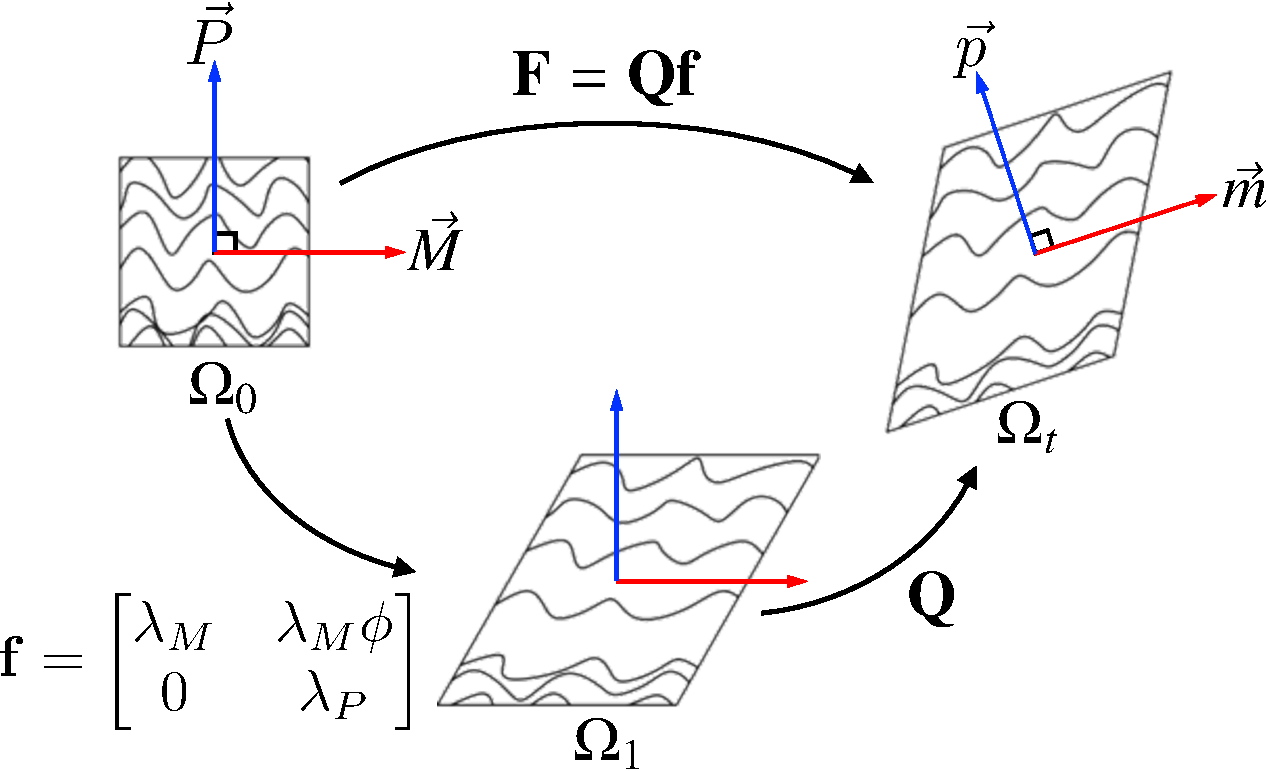
\includegraphics[width=5in]{Images/chapter5/henckykinematics}
\caption{The upper triangular decomposition of the deformation gradient tensor with respect the preferred material axis of soft tissues, whose components are used to define the Hencky strains.}
\label{fig:henckykinematics}
\end{figure}
%-------------------	 end FIGURE 	-------------------%
%%%%%%%%%%%%%%%%%%%%%%%%%%%%%%%%%%%%%%%%%%%%%%%%%%%%%%%%%%%%
    
    
    The Hencky strains can be formulated as followed. Briefly, the upper triangular decomposition, $\mathbf{f}$, when expressed with respect to the material axis of the tissue is given by
%==========================================================%
%-------------------	begin EQUATION 	-------------------%
\begin{equation}
\begin{aligned}
\left[\mathbf{f}\right]_{\mathbf{m}_0,\mathbf{n}_0} = \begin{bmatrix}
\lambda_m 	& \lambda_m\phi \\
0			& \lambda_n
\end{bmatrix}.
\end{aligned}\label{eqn:uppertriangulardecomposition}
\end{equation}
%-------------------	 end EQUATION 	-------------------%
%==========================================================%
    Here, $\mathbf{m}_0$ is the material axis in the referential configuration, which is generally the preferred direction of the fibers embedded in the tissue, $\mathbf{n}_0$ is the direction perpendicular to $\mathbf{m}_0$, $\mathbf{m}_t$ is the material axis in the deformed configuration, $\mathbf{n}_t$ is the direction perpendicular to $\mathbf{m}_t$, $\lambda_m$ and $\lambda_n$ are the stretches along these axes respectively, and $\phi$ is the angle of shear between $\mathbf{m}_0$ and $\mathbf{n}_0$. The corresponding deformation gradient tensor can thus be expressed as 
%==========================================================%
%-------------------	begin EQUATION 	-------------------%
\begin{equation}
\begin{aligned}
\mathbf{F} = \lambda_m\mathbf{m}_t\otimes\mathbf{m}_0 + \lambda_m\phi\mathbf{m}_t\otimes\mathbf{n}_0 + \lambda_n\mathbf{n}_t\otimes\mathbf{n}_0.
\end{aligned}
\end{equation}
%-------------------	 end EQUATION 	-------------------%
%==========================================================%
    The Hencky strains ($\gamma_1, \gamma_2, \gamma_3$), which are functions of the components of $\mathbf{f}$, can be determined using, 
%==========================================================%
%-------------------	begin EQUATION 	-------------------%
\begin{subequations}\label{eqn:henckystrains}
\begin{align}
\gamma_1 &= \log(\lambda_m), &	\gamma_2 &= \log(\lambda_n), 	& \gamma_3 &= \phi	\\
\lambda_m &= \mathbf{m}_t\cdot\mathbf{F}\mathbf{m}_0, &	\lambda_n &= \mathbf{n}_t\cdot\mathbf{F}\mathbf{n}_0,	&	\phi &= \left(\mathbf{m}_t\cdot\mathbf{F}\mathbf{m}_0\right)^{-1}\mathbf{m}_t\cdot\mathbf{F}\mathbf{n}_0.
\end{align}
\end{subequations}
%-------------------	 end EQUATION 	-------------------%
%==========================================================%
    
    
%-------	Hencky vs. Green-Lagrange strain	-------%

	We are most interested in the difference between Green-Lagrange and the Hencky strains for the formulation of the effective constitutive model (Summary Table \ref{tb:greenvshencky}). Firstly, as stated above , Hencky strains lead to a very convenient form for the Cauchy stresses,
%==========================================================%
%-------------------	begin EQUATION 	-------------------%
\begin{equation}\label{eqn:cauchystressform}
\mathbf{T}	= \frac{1}{J} \dpd{\Psi}{\gamma_1} \mathbf{m}_t\otimes\mathbf{m}_t 
			+ \frac{1}{J} \dpd{\Psi}{\gamma_2} \mathbf{n}_t\otimes\mathbf{n}_t 
			+ \frac{\lambda_n}{J\lambda_m} \dpd{\Psi}{\gamma_3} \left(\mathbf{m}_t\otimes\mathbf{n}_t + \mathbf{n}_t\otimes\mathbf{m}_t \right).
%\\
%\dpd{\Psi}{\gamma_1} 	= J \mathbf{m}\cdot\mathbf{T}\mathbf{m}, \quad 
%\dpd{\Psi}{\gamma_2} 	= J \mathbf{s}\cdot\mathbf{T}\mathbf{s}, \quad 
%\dpd{\Psi}{\gamma_3} 	= J \frac{\lambda_m}{\lambda_n}\mathbf{m}\cdot\mathbf{T}\mathbf{s}.
\end{equation}
%-------------------	 end EQUATION 	-------------------%
%==========================================================%
    where $\Psi$ is the strain energy density function. In comparison, the 2nd Piola Kirchhoff stress with Green-Lagrange strains is,
%==========================================================%
%-------------------	begin EQUATION 	-------------------%
\begin{equation} \label{eqn:2ndpkstressform}
\mathbf{S} = \dpd{\Psi}{E_m}\mathbf{m}_0\otimes\mathbf{m}_0
+ \dpd{\Psi}{E_n}\mathbf{n}_0\otimes\mathbf{n}_0 
+ \frac{1}{2}\dpd{\Psi}{E_{\phi}}\left(\mathbf{m}_0\otimes\mathbf{n}_0 + \mathbf{n}_0\otimes\mathbf{m}_0\right),
\end{equation}
%-------------------	 end EQUATION 	-------------------%
%==========================================================%
    with the Cauchy stress obtained from push forward, $\mathbf{T} = (1/J) \mathbf{F}\mathbf{S}\mathbf{F}^\mathsf{T}$. Expressing the Green-Lagrange strain with respect to the material axis, ${E_m, E_n, E_\phi}$, is preferred, so that the model parameters are invariant with respect to rigid body motion and changes in the reference coordinate system. There isn't a significant advantage to either strain measure here. However, we do note that the partial derivative of Green-Lagrange strain, $\pd{\mathbf{E}}{\mathbf{C}}$ (Eqn. \ref{eqn:partialgreens}), is much simpler than that of the Hencky strains, $\pd{\gamma}{\mathbf{C}}$ (Eqn. \ref{eqn:henckyderivatives}). As a result, the elasticity tensor, $\mathbb{C} = C_{ijkl}$, for the Hencky strain is much more complex (see Appendix \ref{sec:elasticitytensor}). 

	One other aspect is the difference in correlation between model parameters when using Green-Lagrange strain, $\{E_m, E_n, E_\phi\}$ vs. using Hencky strains $\{\gamma_1, \gamma_2, \gamma_3 \}$. For example, using the for form of the generalized Fung model,
%==========================================================%
%-------------------	begin EQUATION 	-------------------%
\begin{subequations} \label{eqn:generalizedfungmodel}
\begin{align}
\Psi 	&= c_0 \left(e^{Q} - 1\right),\notag \\
\mathrm{with}	\qquad	Q	&= b_1 E_m^2 + b_2 E_n^2 + b_3 E_\phi^2 + 2 b_4 E_m E_n + 2 b_5 E_mE_\phi + 2 b_6 E_nE_\phi	\label{eqn:generalizedfungmodela} \\ 
\mathrm{or}		\qquad	Q	&= b_1 \gamma_1^2 + b_2 \gamma_2^2 + b_3 \gamma_3^2 + 2 b_4 \gamma_1\gamma_2 + 2 b_5 \gamma_1\gamma_3 + 2 b_6 \gamma_2\gamma_3	\label{eqn:generalizedfungmodelb} 
\end{align}
\end{subequations}
%-------------------	 end EQUATION 	-------------------%
%==========================================================%
    we compared these two strain basis by computing the correlation matrix between the parameters $b_1$ to $b_6$ for the mechanical data acquired from an exogenously cross-linked bovine pericardium specimen \cite{sun_response_2004} (Appendix \ref{sec:parametercorrelation}). The only difference is that we replaced Green Lagrange strain, $E_m$, $E_n$, $E_\phi$ (Eqn. \ref{eqn:generalizedfungmodela}), with the corresponding Hencky strains $\gamma_1$, $\gamma_2$, $\gamma_3$ (Eqn. \ref{eqn:generalizedfungmodelb}) in the model. The correlation between the parameters are mostly similar in both cases, but the Hencky strains come on top with slightly lower correlations, and the determinant of the correlation matrix is higher, $9.38\times10^{-3}$, in comparison to using the Green Lagrange strains, $7.13\times10^{-3}$, (Fig. \ref{fig:gvsecorrelation}, Appendix \ref{sec:parametercorrelation} Table \ref{tb:correlationE} \& \ref{tb:correlationG}). 



%%%%%%%%%%%%%%%%%%%%%%%%%%%%%%%%%%%%%%%%%%%%%%%%%%%%%%%%%%%%
%-------------------	begin FIGURE 	-------------------%
\begin{figure}
\centering
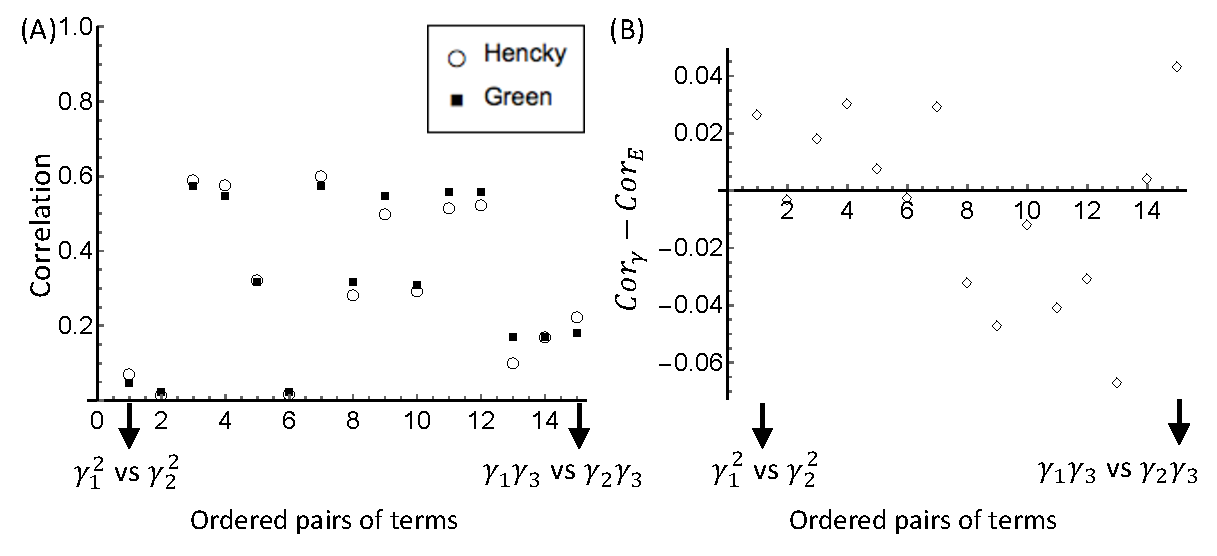
\includegraphics[width=\textwidth]{Images/chapter5/gvsecorrelation}
\caption{(A) The correlation between parameters pairs in the generalized Fung model when using Green-Lagrange vs Hencky strains. (B) The difference in correlation between each pair of parameters, which is very small but with the Hencky strains being lower overall.}
\label{fig:gvsecorrelation}
\end{figure}
%-------------------	 end FIGURE 	-------------------%
%%%%%%%%%%%%%%%%%%%%%%%%%%%%%%%%%%%%%%%%%%%%%%%%%%%%%%%%%%%%

    
    The last and most important difference between Green-Lagrange and Hencky strains is that they handle compression very differently. With the same model form, stresses increase exponentially under compression with Hencky strains, but only mildly with Green-Lagrange strains. We illustrated this again using the generalized Fung model (Eqn. \ref{eqn:generalizedfungmodel}) in the physiologically relevant range, with Green-Lagrange or Hencky strain as the input variable (Fig. \ref{fig:gvsecompression}). The reason for this is actually fairly simple, Green-Lagrange strain maps deformations from $\mathbf{E}: [0,\infty] \rightarrow [-1/2,\infty]$, while Hencky strains maps deformations from $\mathbf{\gamma}: [0,\infty] \rightarrow [-\infty,\infty]$, drastically increasing the magnitude of the same strain value under compression. This behavior very convenient for modeling collageneous tissues, where collagen fibers crimps unload compression but do not increase the stress \cite{soares_mathematical_2017}. Due to all factors considered (Table \ref{tb:greenvshencky}), we proceed to use the Green-Lagrange strain tensor as the best kinematic basis to formulate the effective constitutive model. 
    
    
%%%%%%%%%%%%%%%%%%%%%%%%%%%%%%%%%%%%%%%%%%%%%%%%%%%%%%%%%%%%
%-------------------	begin FIGURE 	-------------------%
\begin{figure}
\centering
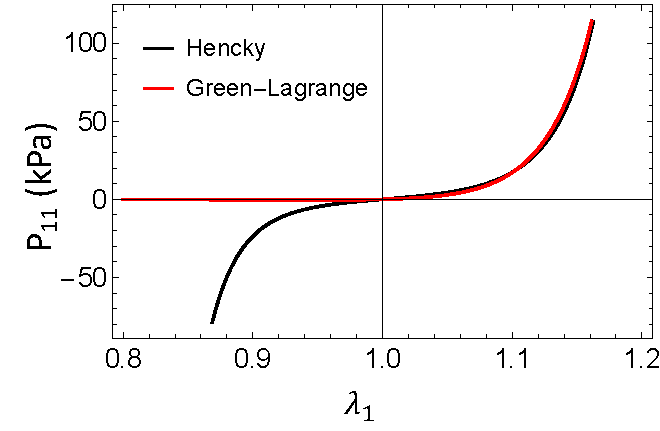
\includegraphics[width=3.25in]{Images/chapter5/gvsecompression}
\caption{The response of a generalized Fung model when using Green-Lagrange (Black) vs Hencky strains(Red). Both models are able to match extensional response nearly perfectly with respect to each other, but drastically differ in response under compression.}
\label{fig:gvsecompression}
\end{figure}
%-------------------	 end FIGURE 	-------------------%
%%%%%%%%%%%%%%%%%%%%%%%%%%%%%%%%%%%%%%%%%%%%%%%%%%%%%%%%%%%%


	





%----------------------------------------------------------%
%-------------------	begin TABLE 	-------------------%
\begin{table}
\caption{The difference between using the Green-Lagrange strain tensor versus the Hencky strains to formulate constitutive models. \textbf{Bold} text indicates key advantages and \textit{Italic} text indicate key disadvantages.}
\begin{center}
\label{tb:greenvshencky}
\begin{tabular}{|L{0.9in}|L{2.25in}|L{2.25in}|}
\hline
\rowcolor{Gray}
\multicolumn{1}{|c|}{Attributes} 
	& \multicolumn{1}{c|}{\textbf{Green-Lagrange strain}} 
    & \multicolumn{1}{c|}{\textbf{Hencky strain}}\\
\hline
General & Most commonly used in modeling	& \textbf{Easy to interpret physically} \\
\hline
Stress 	& Even simpler form for the 2nd Piola Kirchhoff stress \footnotesize
\begin{equation*}
\begin{aligned}
\mathbf{S} =& \dpd{\Psi}{E_m}\mathbf{m}_0\otimes\mathbf{m}_0 + \dpd{\Psi}{E_n}\mathbf{n}_0\otimes\mathbf{n}_0 \\&+ \frac{1}{2}\dpd{\Psi}{E_{\phi}}\left(\mathbf{m}_0\otimes\mathbf{n}_0+\mathbf{n}_0\otimes\mathbf{m}_0\right)
\end{aligned}
\end{equation*}
\normalsize
	& Simple form for the Cauchy stress	\footnotesize
\begin{equation*}
\begin{aligned}
\mathbf{T} =& \dpd{\Psi}{\gamma_{1}}\mathbf{m}_t\otimes\mathbf{m}_t + \dpd{\Psi}{\gamma_{2}}\mathbf{n}_t\otimes\mathbf{n}_t \\ &+ \frac{\lambda_n}{\lambda_m}\dpd{\Psi}{\gamma_{3}}\left(\mathbf{m}_t\otimes\mathbf{n}_t+\mathbf{n}_t\otimes\mathbf{m}_t\right)
\end{aligned}
\end{equation*}
\normalsize
\\
\hline
Elasticity tensor & \textbf{Much simpler form for the elasticity tensor}
	& \textit{The equations for the elasticity tensor is extremely long} \\
\hline
Parameter covariance 	& 	& \textbf{Modestly less correlation between parameters} \\
\hline
Response under compression	&	\textbf{Modest changes in stress under compression, behaves much more similar to soft tissues due to collagen fiber crimp}
	& \textit{Behaves badly under large compression} \begin{itemize}
	\item Log scaling cause the strain energy to increase exponentially with compression
	\end{itemize}\\
\hline
\end{tabular}
\end{center}
\end{table}
%-------------------	 end TABLE 		-------------------%
%----------------------------------------------------------%

%---    METHODS
\section{Elasticity tensor}\label{sec:elasticitytensor}

	An analytical form for the elasticity tensor is extremely important for fast and convergent numerical simulations. A constitutive model without a smooth, continuous, and convex elasticity tensor can pose significant problems for simulation of nonlinear materials to converge quickly, or even to converge at all. The strain basis used for the model can have significant impact on the form of the elasticity tensor. Here, we derived the generalized form of the elasticity tensor for using the Green-Lagrange basis (Eqn. \ref{eqn:greenstrain}) and the Hencky strain basis (Eqn. \ref{eqn:henckystrains}). Note that this is the generalized form, which does not depend on the explicit form of the constitutive model, it is only a function of the strain basis and the response functions (derivatives of the strain energy function), whose form doesn't not have to be explicitly stated. The 9 response functions are:
%=======	BEGIN Equation		=======%
\begin{equation}
\dpd{\Psi}{E_m}, \quad \dpd{\Psi}{E_n}, \quad \dpd{\Psi}{E_\phi}, \quad \frac{\partial^2\Psi}{\partial E_m^2}, \quad \frac{\partial^2\Psi}{\partial E_n^2}, \quad \frac{\partial^2\Psi}{\partial E_\phi^2}, \quad \frac{\partial^2\Psi}{\partial E_m\partial E_n}, \quad \frac{\partial^2\Psi}{\partial E_m\partial E_\phi}, \quad \frac{\partial^2\Psi}{\partial E_n\partial E_\phi}.
\end{equation}
%=======	END Equation		=======%
    
\subsection{Derivation with Green-Lagrange strain}
	
    The elasticity tensor is given by the second derivative of the strain energy function with respect to the right Cauchy strain. Using the chain rules, fully expanding all terms, and enforcing symmetry of partial derivatives, $\md{\Psi}{2}{E_m}{}{E_n}{} = \md{\Psi}{2}{E_n}{}{E_m}{}$, the generalized form for the elasticity tensor is given by 
%=======	BEGIN Equation		=======%
\begin{equation} \label{eqn:generalizedelasticityform}
\begin{aligned}
\dod[2]{\Psi}{\mathbf{C}} =& 
	\dpd{\Psi}{E_m} \dod[2]{E_m}{\mathbf{C}} 
    + \dpd{\Psi}{E_n} \dod[2]{E_n}{\mathbf{C}}
    + \dpd{\Psi}{E_\phi} \dod[2]{E_\phi}{\mathbf{C}} \\
+& \dpd[2]{\Psi}{E_m} \dod{E_m}{\mathbf{C}}\dod{E_m}{\mathbf{C}} 
	+ \dpd[2]{\Psi}{E_n} \dod{E_n}{\mathbf{C}} \dod{E_n}{\mathbf{C}} 
    + \dpd{\Psi}{E_\phi} \dod{E_\phi}{\mathbf{C}} \dod{E_\phi}{\mathbf{C}} \\
+& \dmd{\Psi}{2}{E_m}{}{E_n}{} \left(\dod{E_n}{\mathbf{C}} \dod{E_m}{\mathbf{C}} + \dod{E_m}{\mathbf{C}} \dod{E_n}{\mathbf{C}}\right)   \\
    +& \dmd{\Psi}{2}{E_m}{}{E_\phi}{} \left(\dod{E_\phi}{\mathbf{C}} \dod{E_m}{\mathbf{C}} + \dod{E_m}{\mathbf{C}} \dod{E_\phi}{\mathbf{C}}\right)  \\
    +& \dmd{\Psi}{2}{E_n}{}{E_\phi}{} \left(\dod{E_n}{\mathbf{C}} \dod{E_\phi}{\mathbf{C}} + \dod{E_\phi}{\mathbf{C}} \dod{E_n}{\mathbf{C}}\right).  \\
\end{aligned}
\end{equation}
%=======	END Equation		=======%
To break this down, we begin with the derivatives of the Green-Lagrange strains, which are given by,
%==========================================================%
%-------------------	begin EQUATION 	-------------------%
\begin{equation}\label{eqn:partialgreens}
\begin{aligned}
\dod{E_m}{\mathbf{C}} &= \frac{1}{2} \mathbf{m}\otimes\mathbf{m}	\\
\dod{E_n}{\mathbf{C}} &= \frac{1}{2} \mathbf{n}\otimes\mathbf{n} \\
\dod{E_\phi}{\mathbf{C}} &= \frac{1}{4} \left(\mathbf{m}\otimes\mathbf{n} + \mathbf{n}\otimes\mathbf{m} \right),
\end{aligned}
\end{equation}
%-------------------	 end EQUATION 	-------------------%
%==========================================================%
and 
%==========================================================%
%-------------------	begin EQUATION 	-------------------%
\begin{equation}
\dod[2]{E_m}{\mathbf{C}} = \dod[2]{E_n}{\mathbf{C}} = \dod[2]{E_\phi}{\mathbf{C}} = \mathbf{0}.
\end{equation}
%-------------------	 end EQUATION 	-------------------%
%==========================================================%
Right away, the Green-Lagrange strains have the benefit of the second derivatives being zero, reducing the elasticity tensor (Eqn. \ref{eqn:generalizedelasticityform}) from 9 to 6 terms. Substituting with the partial derivatives (Eqn. \ref{eqn:partialgreens}) gives
%==========================================================%
%-------------------	begin EQUATION 	-------------------%
\begin{equation}\label{eqn:greenelasticityform}
\begin{aligned}
\dod[2]{\Psi}{\mathbf{C}} =
	& \frac{1}{4}\dpd[2]{\Psi}{E_m} \mathbf{m}\otimes\mathbf{m}\otimes\mathbf{m}\otimes\mathbf{m}	\\
    &+ \frac{1}{8}\dmd{\Psi}{2}{E_m}{}{E_\phi}{} 
    	\left(
        	\mathbf{m}\otimes\mathbf{m}\otimes\mathbf{m}\otimes\mathbf{n}
            +\mathbf{m}\otimes\mathbf{m}\otimes\mathbf{n}\otimes\mathbf{m} \right.\\
            &\quad +\left.\mathbf{m}\otimes\mathbf{n}\otimes\mathbf{m}\otimes\mathbf{m}
            +\mathbf{n}\otimes\mathbf{m}\otimes\mathbf{m}\otimes\mathbf{m}
        \right)	\\
    &+ \frac{1}{4}\dmd{\Psi}{2}{E_m}{}{E_n}{} 
    	\left(
        	\mathbf{m}\otimes\mathbf{m}\otimes\mathbf{n}\otimes\mathbf{n}
            +\mathbf{n}\otimes\mathbf{n}\otimes\mathbf{m}\otimes\mathbf{m}
        \right)	\\
    &+ \frac{1}{16}\dpd[2]{\Psi}{E_\phi} 
    	\left(
        	\mathbf{m}\otimes\mathbf{n}\otimes\mathbf{m}\otimes\mathbf{n}
            +\mathbf{m}\otimes\mathbf{n}\otimes\mathbf{n}\otimes\mathbf{m} \right. \\
            &\quad \left.+\mathbf{n}\otimes\mathbf{m}\otimes\mathbf{m}\otimes\mathbf{n}
            +\mathbf{n}\otimes\mathbf{m}\otimes\mathbf{n}\otimes\mathbf{m}
        \right)	\\
    &+ \frac{1}{8}\dmd{\Psi}{2}{E_n}{}{E_\phi}{} 
    	\left(
        	\mathbf{m}\otimes\mathbf{n}\otimes\mathbf{n}\otimes\mathbf{n}
            +\mathbf{n}\otimes\mathbf{m}\otimes\mathbf{n}\otimes\mathbf{n} \right. \\
            &\quad +\left. \mathbf{n}\otimes\mathbf{n}\otimes\mathbf{m}\otimes\mathbf{n}
            +\mathbf{n}\otimes\mathbf{n}\otimes\mathbf{n}\otimes\mathbf{m}
        \right)	\\
    &+ \frac{1}{4} \dpd[2]{\Psi}{E_n} \mathbf{n}\otimes\mathbf{n}\otimes\mathbf{n}\otimes\mathbf{n}	\\
\end{aligned}
\end{equation}
%-------------------	 end EQUATION 	-------------------%
%==========================================================%


\subsection{Derivation with Hencky strains}

	The elasticity tensor when using the Hencky strains is much more complex. For start, the second derivatives of the Hencky strains are non-zero. The derivatives themselves are complex both in form and conceptually. The derivation of the derivatives is not straight forward. To make this simpler, we start with an alternative definition for the Hencky strains, which relates the 4 variables, $\gamma_1$, $\gamma_2$, $\gamma_3$, and $\mathbf{C}$.  
%==========================================================%
%-------------------	begin EQUATION 	-------------------%
\begin{equation}\label{eqn:invariantset}
\begin{aligned}
    \gamma_1 &= \ln \left( \lambda_m \right), &  \lambda_m^2 &= \mathbf{m}\cdot\mathbf{C}\mathbf{m}  \\
    \gamma_2 &= \ln \left( \lambda_n \right), &  \lambda_n^2 &= \mathbf{n}\cdot\mathbf{C}\mathbf{n} 
                    - \lambda_m^2 \phi^2   \\
    \gamma_3 &= \phi, & \phi &= \left( \lambda_m\right)^{-2}\mathbf{m}\cdot\mathbf{C}\mathbf{n}.
\end{aligned}
\end{equation}
%-------------------	 end EQUATION 	-------------------%
%==========================================================%
It is important here that with this definition, the vector basis, $\mathbf{m}$ and $\mathbf{n}$, are defined on the reference coordinate system, which does not change with deformation. By chain rule, the first derivatives are as followed,
%==========================================================%
%-------------------	begin EQUATION 	-------------------%
\begin{subequations}
\begin{align}
\dod{\gamma_1}{\mathbf{C}} =& \dpd{\gamma_1}{\lambda_m}\dod{\lambda_m}{\mathbf{C}},	
	& \dod{\lambda_m^2}{\mathbf{C}} =& \dpd{\lambda_m^2}{\mathbf{C}}:\dod{\mathbf{C}}{\mathbf{C}} 
	+ \dpd{\lambda_m^2}{\lambda_n}\dod{\lambda_n}{\mathbf{C}}
    + \dpd{\lambda_m^2}{\phi}\dod{\phi}{\mathbf{C}} \\
\dod{\gamma_2}{\mathbf{C}} =& \dpd{\gamma_2}{\lambda_n}\dod{\lambda_n}{\mathbf{C}},	
	& \dod{\lambda_n^2}{\mathbf{C}} =& \dpd{\lambda_n^2}{\mathbf{C}}:\dod{\mathbf{C}}{\mathbf{C}} 
	+ \dpd{\lambda_n^2}{\lambda_m}\dod{\lambda_m}{\mathbf{C}}
    + \dpd{\lambda_n^2}{\phi}\dod{\phi}{\mathbf{C}} \\
\dod{\gamma_3}{\mathbf{C}} =& \dod{\phi}{\mathbf{C}},
	& \dod{\phi}{\mathbf{C}} =& \dpd{\phi}{\mathbf{C}}:\dod{\mathbf{C}}{\mathbf{C}} 
	+ \dpd{\phi}{\lambda_m}\dod{\lambda_m}{\mathbf{C}}
    + \dpd{\phi}{\lambda_n}\dod{\lambda_n}{\mathbf{C}}. 
\end{align}
\end{subequations}
%-------------------	 end EQUATION 	-------------------%
%==========================================================%
First, note that all the partial derivatives are functions of each other. This is indeed problematic, but also note from equation \ref{eqn:invariantset} that $\lambda_m$ does not depend on $\lambda_n$ and $\phi$, and $\phi$ does not depend on $\lambda_n$. This means that the following partial derivatives are zero,
%==========================================================%
%-------------------	begin EQUATION 	-------------------%
\begin{equation}\label{eqn:henckystraindependence}
\begin{aligned}
\dpd{\lambda_m}{\lambda_n} = \dpd{\lambda_m}{\phi} = \dpd{\phi}{\lambda_n} = 0,
\end{aligned}
\end{equation}
%-------------------	 end EQUATION 	-------------------%
%==========================================================%
allowing the equations to be solved. 

	For the second derivatives, note from the definition we have above, the Hencky strains are only linear function of $\mathbf{C}$, thus their 2nd \emph{partial derivatives} are zero with respect to $\mathbf{C}$ only,
%==========================================================%
%-------------------	begin EQUATION 	-------------------%
\begin{equation}
\begin{aligned}
\dpd{}{\mathbf{C}}\left(\dod{\gamma_1}{\mathbf{C}}\right) 
	=\dpd{}{\mathbf{C}}\left(\dod{\gamma_2}{\mathbf{C}}\right)
    =\dpd{}{\mathbf{C}}\left(\dod{\gamma_3}{\mathbf{C}}\right)
    =0.
\end{aligned}
\end{equation}
%-------------------	 end EQUATION 	-------------------%
%==========================================================%
The second derivatives are thus defined to be,
%==========================================================%
%-------------------	begin EQUATION 	-------------------%
\begin{subequations}
\begin{align}
\dod{}{\mathbf{C}}\left(\dod{\gamma_1}{\mathbf{C}}\right) =&
    \dpd{}{\lambda_m}\left(\dod{\gamma_1}{\mathbf{C}}\right)\dod{\lambda_m}{\mathbf{C}}
    + \dpd{}{\lambda_n}\left(\dod{\gamma_1}{\mathbf{C}}\right)\dod{\lambda_n}{\mathbf{C}}
    + \dpd{}{\phi}\left(\dod{\gamma_1}{\mathbf{C}}\right)\dod{\phi}{\mathbf{C}}	\\
\dod{}{\mathbf{C}}\left(\dod{\gamma_2}{\mathbf{C}}\right) =&
    \dpd{}{\lambda_m}\left(\dod{\gamma_2}{\mathbf{C}}\right)\dod{\lambda_m}{\mathbf{C}}
    + \dpd{}{\lambda_n}\left(\dod{\gamma_2}{\mathbf{C}}\right)\dod{\lambda_n}{\mathbf{C}}
    + \dpd{}{\phi}\left(\dod{\gamma_2}{\mathbf{C}}\right)\dod{\phi}{\mathbf{C}}	\\
\dod{}{\mathbf{C}}\left(\dod{\phi}{\mathbf{C}}\right) =&
    \dpd{}{\lambda_m}\left(\dod{\phi}{\mathbf{C}}\right)\dod{\lambda_m}{\mathbf{C}}
    + \dpd{}{\lambda_n}\left(\dod{\phi}{\mathbf{C}}\right)\dod{\lambda_n}{\mathbf{C}}
    + \dpd{}{\phi}\left(\dod{\phi}{\mathbf{C}}\right)\dod{\phi}{\mathbf{C}} 
\end{align}
\end{subequations}
%-------------------	 end EQUATION 	-------------------%
%==========================================================%
Taking advantage of equation \ref{eqn:henckystraindependence}, the first and second derivatives of the Hencky strains are presented as followed:
%==========================================================%
%-------------------	begin EQUATION 	-------------------%
\begin{subequations} \label{eqn:henckyderivatives}
\begin{align}
\dod{\gamma_1}{\mathbf{C}} =& \frac{1}{2\lambda_m^2} \mathbf{m}\otimes\mathbf{m}	\\
\dod{\gamma_2}{\mathbf{C}} =& \frac{1}{2\lambda_n^2} \left(\mathbf{n}\otimes\mathbf{n} - \phi \left( \mathbf{m}\otimes\mathbf{n} + \mathbf{n}\otimes\mathbf{m}\right) + \phi^2 \mathbf{m}\otimes\mathbf{m} \right)	\\
\dod{\gamma_3}{\mathbf{C}} =& \frac{1}{2\lambda_m^2} \left( \mathbf{m}\otimes\mathbf{n} + \mathbf{n}\otimes\mathbf{m} - 2\phi \mathbf{m}\otimes\mathbf{m}\right) \\
\dod[2]{\gamma_1}{\mathbf{C}} =& -\frac{1}{2}\frac{1}{\lambda_m^4}\mathbf{m}\otimes\mathbf{m} \otimes \mathbf{m}\otimes\mathbf{m}	\\
\begin{split}
\dod[2]{\gamma_2}{\mathbf{C}} =& -\frac{1}{2}\frac{1}{\lambda_n^4} 
    \left[
    \mathbf{n}\otimes\mathbf{n}\otimes\mathbf{n}\otimes\mathbf{n}
    -\phi \mathbf{m}\otimes\mathbf{n}\otimes\mathbf{n}\otimes\mathbf{n}
    -\phi \mathbf{n}\otimes\mathbf{m}\otimes\mathbf{n}\otimes\mathbf{n}\right.   \\
    &-\phi \mathbf{n}\otimes\mathbf{n}\otimes\mathbf{m}\otimes\mathbf{n}
    -\phi \mathbf{n}\otimes\mathbf{n}\otimes\mathbf{n}\otimes\mathbf{m}   
    +\phi^2 \mathbf{m}\otimes\mathbf{m}\otimes\mathbf{n}\otimes\mathbf{n} \\
    &\left.+\phi^2 \mathbf{n}\otimes\mathbf{n}\otimes\mathbf{m}\otimes\mathbf{m}
    \right]\\
    &-\left(\frac{1}{4}\frac{1}{\lambda_m^2\lambda_n^2} + \frac{1}{2}\phi^2\frac{1}{\lambda_n^4} \right)
    \left[
    \mathbf{m}\otimes\mathbf{n}\otimes\mathbf{m}\otimes\mathbf{n}
    +\mathbf{m}\otimes\mathbf{n}\otimes\mathbf{n}\otimes\mathbf{m} \right. \\
    &+\left. \mathbf{n}\otimes\mathbf{m}\otimes\mathbf{m}\otimes\mathbf{n}
    +\mathbf{n}\otimes\mathbf{m}\otimes\mathbf{n}\otimes\mathbf{m}
    \right]\\
    &+\left(\frac{1}{2}\phi\frac{1}{\lambda_m^2\lambda_n^2} + \frac{1}{2}\phi^3\frac{1}{\lambda_n^4} \right)
    \left[
    \mathbf{m}\otimes\mathbf{m}\otimes\mathbf{m}\otimes\mathbf{n}
    +\mathbf{m}\otimes\mathbf{m}\otimes\mathbf{n}\otimes\mathbf{m} \right. \\
    &+\left. \mathbf{m}\otimes\mathbf{n}\otimes\mathbf{m}\otimes\mathbf{m}
    +\mathbf{n}\otimes\mathbf{m}\otimes\mathbf{m}\otimes\mathbf{m}
    \right]\\
    &-\left(\phi^2\frac{1}{\lambda_m^2\lambda_n^2} + \frac{1}{2}\phi^4\frac{1}{\lambda_n^4} \right)
    \left[
    \mathbf{m}\otimes\mathbf{m}\otimes\mathbf{m}\otimes\mathbf{m}
    \right]
\end{split}\\
\begin{split}
\dod[2]{\gamma_3}{\mathbf{C}} =& -\frac{1}{2}\frac{1}{\lambda_m^4} \times \left(
        \mathbf{n}\otimes\mathbf{m}\otimes\mathbf{m}\otimes\mathbf{m} + \mathbf{m}\otimes\mathbf{n}\otimes\mathbf{m}\otimes\mathbf{m}\right. \\
        &+ \left.\mathbf{m}\otimes\mathbf{m}\otimes\mathbf{n}\otimes\mathbf{m} +
        \mathbf{m}\otimes\mathbf{m}\otimes\mathbf{m}\otimes\mathbf{n} - 
        4\phi\mathbf{m}\otimes\mathbf{m} \otimes \mathbf{m}\otimes\mathbf{m} \right)
\end{split}
\end{align}
\end{subequations}
%-------------------	 end EQUATION 	-------------------%
%==========================================================%

	Saving everyone from the algebra, without further ado, the most elegant form of the elasticity tensor for constitutive models based on the Hencky strains is, 
%==========================================================%
%-------------------	begin EQUATION 	-------------------%
\begin{subequations} \label{eqn:elasticityhencky}
\begin{align}
\begin{split}
\dod[2]{\Psi}{\mathbf{C}} =&
	\psi_1 \mathbf{m}\otimes\mathbf{m}\otimes\mathbf{m}\otimes\mathbf{m}	\\
    &+ \psi_2
    	\left(
        	\mathbf{m}\otimes\mathbf{m}\otimes\mathbf{m}\otimes\mathbf{n}
            +\mathbf{m}\otimes\mathbf{m}\otimes\mathbf{n}\otimes\mathbf{m} \right. \\
            &\quad +\left. \mathbf{m}\otimes\mathbf{n}\otimes\mathbf{m}\otimes\mathbf{m}
            +\mathbf{n}\otimes\mathbf{m}\otimes\mathbf{m}\otimes\mathbf{m}
        \right)	\\
    &+ \psi_3
    	\left(
        	\mathbf{m}\otimes\mathbf{m}\otimes\mathbf{n}\otimes\mathbf{n}
            +\mathbf{n}\otimes\mathbf{n}\otimes\mathbf{m}\otimes\mathbf{m}
        \right)	\\
    &+ \psi_4
    	\left(
        	\mathbf{m}\otimes\mathbf{n}\otimes\mathbf{m}\otimes\mathbf{n}
            +\mathbf{m}\otimes\mathbf{n}\otimes\mathbf{n}\otimes\mathbf{m} \right. \\
            &\quad +\left.\mathbf{n}\otimes\mathbf{m}\otimes\mathbf{m}\otimes\mathbf{n}
            +\mathbf{n}\otimes\mathbf{m}\otimes\mathbf{n}\otimes\mathbf{m}
        \right)	\\
    &+ \psi_5
    	\left(
        	\mathbf{m}\otimes\mathbf{n}\otimes\mathbf{n}\otimes\mathbf{n}
            +\mathbf{n}\otimes\mathbf{m}\otimes\mathbf{n}\otimes\mathbf{n}
            +\mathbf{n}\otimes\mathbf{n}\otimes\mathbf{m}\otimes\mathbf{n}
            +\mathbf{n}\otimes\mathbf{n}\otimes\mathbf{n}\otimes\mathbf{m}
        \right)	\\
    &+ \psi_6 \mathbf{n}\otimes\mathbf{n}\otimes\mathbf{n}\otimes\mathbf{n}
\end{split}	\\
\begin{split}
\psi_1 =&
        -\frac{1}{2}\frac{1}{\lambda_m^4}W^{(1)}
        -\left(\frac{\phi^2}{\lambda_m^2\lambda_n^2}+\frac{1}{2}\frac{\phi^4}{\lambda_n^4}\right)W^{(2)}
        +2\frac{\phi}{\lambda_m^4}W^{(3)}
        +\frac{1}{4}\frac{1}{\lambda_m^4}W^{(11)}   \\
        &+\frac{1}{4}\frac{\phi^4}{\lambda_n^4}W^{(22)}
        +\frac{\phi^2}{\lambda_m^4}W^{(33)}
        +\frac{1}{2}\frac{\phi^2}{\lambda_m^2\lambda_n^2}W^{(12)}
        -\frac{\phi}{\lambda_m^4}W^{(13)}
        -\frac{\phi^3}{\lambda_m^2 \lambda_n^2}W^{(23)}
\end{split}	\\
\begin{split}
\psi_2 =&
        \frac{1}{2}\left(\frac{\phi}{\lambda_m^2\lambda_n^2} + \frac{\phi^3}{\lambda_n^4}\right)W^{(2)}
        -\frac{1}{2}\frac{1}{\lambda_m^4}W^{(3)}
        -\frac{1}{4}\frac{\phi^3}{\lambda_n^4}W^{(22)}
        -\frac{1}{2}\frac{\phi}{\lambda_m^4}W^{(33)}    \\
        &-\frac{1}{4}\frac{\phi}{\lambda_m^2 \lambda_n^2}W^{(12)}
        +\frac{1}{4}\frac{1}{\lambda_m^4}W^{(13)}
        +\frac{3}{4}\frac{\phi^2}{\lambda_m^2 \lambda_n^2}W^{(23)}
\end{split}	\\
\psi_3 =&
        -\frac{1}{2}\frac{\phi^2}{\lambda_n^4}W^{(2)}
        +\frac{1}{4}\frac{\phi^2}{\lambda_n^4}W^{(22)}
        +\frac{1}{4}\frac{1}{\lambda_m^2 \lambda_n^2}W^{(12)}
        -\frac{1}{2}\frac{\phi}{\lambda_m^2 \lambda_n^2}W^{(23)}	\\
\psi_4 =&
        -\left(\frac{1}{4}\frac{1}{\lambda_m^2\lambda_n^2}+\frac{1}{2}\frac{\phi^2}{\lambda_n^4}\right)W^{(2)}
        +\frac{1}{4}\frac{\phi^2}{\lambda_n^4}W^{(22)}
        +\frac{1}{4}\frac{1}{\lambda_m^4}W^{(33)}
        -\frac{1}{2}\frac{\phi}{\lambda_m^2 \lambda_n^2}W^{(23)}	\\
\psi_5 =&
        \frac{1}{2}\frac{\phi}{\lambda_n^4}W^{(2)}
        -\frac{1}{4}\frac{\phi}{\lambda_n^4}W^{(22)}
        +\frac{1}{4}\frac{1}{\lambda_m^2 \lambda_n^2}W^{(23)}	\\
\psi_6 =&
        -\frac{1}{2}\frac{1}{\lambda_n^4}W^{(2)}
        +\frac{1}{4}\frac{1}{\lambda_n^4}W^{(22)}
\end{align}
\end{subequations}
%-------------------	 end EQUATION 	-------------------%
%==========================================================%
where $W^{ij} = \md{\Psi}{2}{\gamma_i}{}{\gamma_j}{}$.

\paragraph{Some final remarks} 
	The elasticity tensor for the Hencky strains (Eqn. \ref{eqn:elasticityhencky}) are somewhat complicated, but most terms are weighted by $\gamma_3$, which is the shear angle $\phi$. Under no shear, the form for the elasticity tensor reduces significantly, to similar in form to the Green-Lagrange strains (Eqn. \ref{eqn:greenelasticityform}). The shear angle is typically a small value as well, making most terms in the elasticity tensor small as well. However, they are still necessary to accurately compute the elasticity tensor and are representative of the coupling between the strains components. 
    
    More interesting is perhaps that the Hencky strains overall leads to less covariance in model parameters overall, despite there being many more coupling terms than the Green-Lagrange strain. This is indicative of the covariance within the model form and of the tissue, which in turn is necessary to reproduce soft tissue responses. Due to this natural covariance of the tissues themselves, truly non-covariant models are not feasibly attainable. The level of covariance demonstrated by $\Psi_{eff}$ (Eqn. \ref{eqn:finalexponentialmodelformscaled}) within are likely close to optimal without sacrificing for addition model complexity. 



















% loss of benefits for the correlation between parameters from polynomial to exponential model. 

%---    Results
\section{Parameter correlation}\label{sec:parametercorrelation}

	The Fisher's information matrix for a maximum likelihood problem described by a multivariate normally distributed statistical model is defined to be the negative of the second partial derivatives of the log-likelihood function with respect to the parameters, $\xi_i$, evaluated at the maximum likelihood estimates. When converting to least squares minimization, which is equivalent of a negative log-likelihood minimization, the information matrix is defined to be
%==========================================================%
%-------------------	begin EQUATION 	-------------------%
\begin{equation}\label{eqn:informationmatrix}
\begin{aligned}
\mathcal{I}_{jk} = \dmd{\mathcal{F}}{2}{\xi_j}{}{\xi_k}{} = \mathcal{H}_{jk},
\end{aligned}
\end{equation}
%-------------------	 end EQUATION 	-------------------%
%==========================================================%
which is also exactly the Hessian matrix, $\mathbfcal{H}$, at the best fit value. The D-optimality is the determinant of this information matrix, whereas other optimality measures are mostly similar functions of this information matrix. The main reason is because, for a maximum likelihood problem governed by a normally distributed statistical model, the covariance matrix is exactly proportional to the inverse of the information matrix,
%==========================================================%
%-------------------	begin EQUATION 	-------------------%
\begin{equation}\label{eqn:covariancematrix}
\begin{aligned}
\mathbf{Cov} = \sigma^2 \mathbfcal{I}^{-1},
\end{aligned}
\end{equation}
%-------------------	 end EQUATION 	-------------------%
%==========================================================%
where $\sigma^2$ is the scalar variance of the statistical model, and can be estimated by the mean squared error weighted by the degree of freedom. Maximizing the D-optimality is equivalent of minimizing the variance of each parameter along with minimizing the covariance between parameters. Defining the objective function as
%==========================================================%
%-------------------	begin EQUATION 	-------------------%
\begin{equation}
\begin{aligned}
\mathcal{F} = \sum_i \left(f(x_i) - f_i\right)^2,
\end{aligned}
\end{equation}
%-------------------	 end EQUATION 	-------------------%
%----------------------------------------------------------%
where $f(x_i)$ is the model and $f_i$ are date points, the information matrix, or Hessian matrix, is given by 
%==========================================================%
%-------------------	begin EQUATION 	-------------------%
\begin{equation}\label{eqn:hessianmatrix}
\begin{aligned}
\dpd{\mathcal{F}}{\xi_j} =& \sum_i 2\left(f(x_i) - f_i\right)\dpd{f(x_i)}{\xi_j}	\\
\mathcal{H}_{jk} = \dmd{\mathcal{F}}{2}{\xi_j}{}{\xi_k}{} =& \sum_i 2\dpd{f(x_i)}{\xi_k}\dpd{f(x_i)}{\xi_j}	+ 2\left(f(x_i) - f_i\right)\dmd{f(x_i)}{2}{\xi_j}{}{\xi_k}{}
\end{aligned}
\end{equation}
%-------------------	 end EQUATION 	-------------------%
%----------------------------------------------------------%
Note here that $\mathcal{J}_{ij} = \dpd{f(x_i)}{\xi_j}$ is the Jacobian matrix for the non-linear least squares problem, and when the errors are small, i.e. when the model fits the data, in other words such that $\left(f(x_i) - f_i\right)$ is small or approximately 0, then the information matrix can by approximated by  
\begin{equation}
\mathcal{I}_{jk} \approx \mathcal{J}_{ji}\mathcal{J}_{ik} \quad \mathrm{or} \quad
\mathbfcal{I} \approx \mathbfcal{J}^\mathsf{T}\mathbfcal{J},
\end{equation}
a form much more familiar to most doing nonlinear least squares parameter estimation. 


	For $\Psi_{eff}$ (Eqn. \ref{eqn:finalexponentialmodelformscaled}), let $f = c_0Q^\prime e^{Q}$ be the stress, where $Q^\prime$ is one of $\pd{Q}{E_m}$, $\pd{Q}{E_n}$, or $\pd{Q}{E_\phi}$. The Jacobian matrix is thus, 
\begin{equation}	
\mathcal{J}_{ij} = Q^\prime e^Q \delta_{0j} + c_0 e^Q \dpd{Q^\prime}{\xi_j}+ c_0Q^\prime e^Q \dpd{Q}{\xi_j}
\end{equation}
Note that since $Q$ is a sum of polynomials, the second partial derivatives of $Q$ and $Q^\prime$ with respect to $\mathbf{\xi}$ is precisely 0,
\begin{equation}		
\md{Q}{2}{\xi_j}{}{\xi_k}{}  = \md{Q^\prime}{2}{\xi_j}{}{\xi_k}{} = 0.
\end{equation}
Thus,
\begin{equation}	
\begin{aligned}
\dmd{f}{2}{\xi_j}{}{\xi_k}{} =& e^Q \delta_{0j}\dpd{Q^\prime}{\xi_k} + Q^\prime e^Q \delta_{0j}\dpd{Q}{\xi_k} 
+  e^Q\dpd{Q^\prime}{\xi_j}\delta_{0k} + c_0 e^Q\dpd{Q^\prime}{\xi_j}\dpd{Q}{\xi_k} 
+ Q^\prime e^Q \dpd{Q}{\xi_j}\delta_{0k} 	\\
&+ c_0e^Q \dpd{Q}{\xi_j}\dpd{Q^\prime}{\xi_k}
+ c_0Q^\prime e^Q \dpd{Q}{\xi_j}\dpd{Q}{\xi_k} 
\end{aligned}
\end{equation}
and the Hessian matrix is given by
% \begin{equation}	
% \begin{aligned}
% \mathcal{H}_{jk} &= 2\sum_i\left[ (Q^\prime e^Q)^2  \delta_{0j}\delta_{0k} + c_0Q^\prime e^{2Q} \delta_{0j}\dpd{Q^\prime}{\xi_k}+ c_0 (Q^\prime e^Q)^2 \delta_{0j}\dpd{Q}{\xi_k}\right.	\\
% &+c_0Q^\prime e^{2Q} \dpd{Q^\prime}{\xi_j} \delta_{0k} + (c_0 e^Q)^2 \dpd{Q^\prime}{\xi_j}\dpd{Q^\prime}{\xi_k}+ (c_0e^Q)^2Q^\prime  \dpd{Q^\prime}{\xi_j}\dpd{Q}{\xi_k}	\\
% &+ c_0(Q^\prime e^Q)^2 \dpd{Q}{\xi_j}\delta_{0k} + Q^\prime (c_0 e^Q)^2 \dpd{Q}{\xi_j}\dpd{Q^\prime}{\xi_k}+ (c_0Q^\prime e^Q)^2 \dpd{Q}{\xi_j}\dpd{Q}{\xi_k}	\\
% &+ (c_0Q^\prime e^Q - f_i)\left( e^Q \delta_{0j}\dpd{Q^\prime}{\xi_k} + Q^\prime e^Q \delta_{0j}\dpd{Q}{\xi_k} 
% +  e^Q\dpd{Q^\prime}{\xi_j}\delta_{0k} 
% \right.	\\
% &\left.\left.+ c_0 e^Q\dpd{Q^\prime}{\xi_j}\dpd{Q}{\xi_k} + Q^\prime e^Q \dpd{Q}{\xi_j}\delta_{0k}  + c_0e^Q \dpd{Q}{\xi_j}\dpd{Q^\prime}{\xi_k}
% + c_0Q^\prime e^Q \dpd{Q}{\xi_j}\dpd{Q}{\xi_k} \right)\right]
% \end{aligned}
% \end{equation}

\begin{equation}	
\begin{aligned}
\mathcal{H}_{jk} &= 2\sum_i\left[ (Q^\prime e^Q)^2  \delta_{0j}\delta_{0k} + c_0Q^\prime e^{2Q} \left(\delta_{0j}\dpd{Q^\prime}{\xi_k} + \dpd{Q^\prime}{\xi_j} \delta_{0k}\right) \right.	\\
&+ c_0 (Q^\prime e^Q)^2 \left(\delta_{0j}\dpd{Q}{\xi_k} + \dpd{Q}{\xi_j}\delta_{0k}\right) + (c_0 e^Q)^2 \dpd{Q^\prime}{\xi_j}\dpd{Q^\prime}{\xi_k} \\
&+  (c_0e^Q)^2Q^\prime \left( \dpd{Q^\prime}{\xi_j}\dpd{Q}{\xi_k}	+ \dpd{Q}{\xi_j}\dpd{Q^\prime}{\xi_k}\right) + (c_0Q^\prime e^Q)^2 \dpd{Q}{\xi_j}\dpd{Q}{\xi_k} \\
&+ (c_0Q^\prime e^Q - f_i)\left.\left[ e^Q \left(\delta_{0j}\dpd{Q^\prime}{\xi_k} + \dpd{Q^\prime}{\xi_j}\delta_{0k}\right) + Q^\prime e^Q \left(\delta_{0j}\dpd{Q}{\xi_k}  + \dpd{Q}{\xi_j}\delta_{0k}\right)
\right.\right.	\\
&\left.\left.+ c_0 e^Q\left(\dpd{Q^\prime}{\xi_j}\dpd{Q}{\xi_k}  +  \dpd{Q}{\xi_j}\dpd{Q^\prime}{\xi_k}\right)
+ c_0Q^\prime e^Q \dpd{Q}{\xi_j}\dpd{Q}{\xi_k} \right]\right].
\end{aligned}
\end{equation}
Here, the summation is over each data point $i$ and then sums for each component of stress $S_m$, $S_n$, and $S_\phi$ for $Q^\prime = \pd{Q}{E_m}$, $\pd{Q}{E_n}$ and $\pd{Q}{E_\phi}$ respectively. 

	Using this approach, we compared the covariance of the model parameters for with Green-Lagrange strains and with Hencky strains for the Fung model (Table \ref{tb:correlationE}\&\ref{tb:correlationG}, Fig. \ref{fig:gvsecorrelation}), $\Psi_{eff}$ (Eqn. \ref{eqn:finalexponentialmodelformscaled}) (Fig. \ref{fig:gvsecorrelationeff}), and the polynomial series type model with $i,j,k \leq 6$ (Fig. \ref{fig:gvsecorrelationpoly}). The Hencky strains have lower parameter correlation as shown, but this appears to be minimal for $\Psi_{eff}$. The main benefits are seen with higher order coupling terms, and may still be beneficial for other constitutive models forms. 



%----------------------------------------------------------%
%-------------------	begin TABLE 	-------------------%
\begin{table}[ht]
\caption{The correlation between model parameter when using Green Lagrange strains}
\begin{center}
\label{tb:correlationE}
\small 
\begin{tabular}{|l|cccccc|}
\hline
		 & $b_1$ & $b_2$& $b_3$& $b_4$& $b_5$& $b_6$ \\
\hline  
$b_1$	 & 1. & 0.0439916 & 0.0195981 & -0.571707 & -0.545413 & 0.314503 \\
$b_2$	 & 0.0439916 & 1. & 0.0195981 & -0.571707 & 0.314503 & -0.545413 \\
$b_3$	 & 0.0195981 & 0.0195981 & 1. & 0.306268 & -0.555437 & -0.555437 \\
$b_4$	 & -0.571707 & -0.571707 & 0.306268 & 1. & -0.167068 & -0.167068 \\
$b_5$	 & -0.545413 & 0.314503 & -0.555437 & -0.167068 & 1. & -0.179471 \\
$b_6$	 & 0.314503 & -0.545413 & -0.555437 & -0.167068 & -0.179471 & 1. \\
\hline
\end{tabular}
\normalsize
\end{center}
\end{table}
%-------------------	 end TABLE 		-------------------%
%----------------------------------------------------------%


%----------------------------------------------------------%
%-------------------	begin TABLE 	-------------------%
\begin{table}[ht]
\caption{The correlation between model parameter when using Hencky strains}
\begin{center}
\label{tb:correlationG}
\small
\begin{tabular}{|l|cccccc|}
\hline
		& $b_1$ & $b_2$& $b_3$& $b_4$& $b_5$& $b_6$ \\
\hline
$b_1$	& 1. & 0.0709169 & 0.016636 & -0.590101 & -0.576084 & 0.322457 \\
$b_2$	& 0.0709169 & 1. & -0.0173651 & -0.601126 & 0.282699 & -0.49857 \\
$b_3$	& 0.016636 & -0.0173651 & 1. & 0.294546 & -0.514879 & -0.524943 \\
$b_4$	& -0.590101 & -0.601126 & 0.294546 & 1. & -0.100413 & -0.171661 \\
$b_5$	& -0.576084 & 0.282699 & -0.514879 & -0.100413 & 1. & -0.222942 \\
$b_6$	& 0.322457 & -0.49857 & -0.524943 & -0.171661 & -0.222942 & 1. \\
\hline
\end{tabular}
\normalsize
\end{center}
\end{table}
%-------------------	 end TABLE 		-------------------%
%----------------------------------------------------------%


%%%%%%%%%%%%%%%%%%%%%%%%%%%%%%%%%%%%%%%%%%%%%%%%%%%%%%%%%%%%
%-------------------	begin FIGURE 	-------------------%
\begin{figure}
\centering
\includegraphics[width=6.0in]{Images/chapter5/gvsecorrelationeff}
\caption{(A) The correlation between parameters pairs in $\Psi_{eff}$ (Eqn. \ref{eqn:finalexponentialmodelformscaled}) when using Green-Lagrange vs Hencky strains. (B) The difference in correlation between each pair of parameters is minimal.}
\label{fig:gvsecorrelationeff}
\end{figure}
%-------------------	 end FIGURE 	-------------------%
%%%%%%%%%%%%%%%%%%%%%%%%%%%%%%%%%%%%%%%%%%%%%%%%%%%%%%%%%%%%


%%%%%%%%%%%%%%%%%%%%%%%%%%%%%%%%%%%%%%%%%%%%%%%%%%%%%%%%%%%%
%-------------------	begin FIGURE 	-------------------%
\begin{figure}
\centering
\includegraphics[width=\textwidth]{Images/chapter5/gvsecorrelationpoly}
\caption{(A) The correlation between parameters pairs in a polynomial series type model with powers up to 6 when using Green-Lagrange vs (B) Hencky strains. (C) The difference in correlation between each pair of parameters. The red bracketed terms are benefited from using Hencky strains whereas the significantly fewer blue bracketed terms has better correlations with Green-Lagrange strain.}
\label{fig:gvsecorrelationpoly}
\end{figure}
%-------------------	 end FIGURE 	-------------------%
%%%%%%%%%%%%%%%%%%%%%%%%%%%%%%%%%%%%%%%%%%%%%%%%%%%%%%%%%%%%
















%---    Discussion
\section{Optimal \textit{in silico} loading paths} \label{sec:optimalpaths}

	The most optimal loading path is the equibiaxial stress loading paths. This is not surprising as the equibiaxial stress response generally given very intuitive information on the mechanical response of soft tissues. Any odd number of loading paths will include the equibiaxial stress loading paths (Fig. \ref{fig:oddpaths}). Even when the number is even, we can observe that at least a few protocols are nearly equibiaxial in stress (Fig. \ref{fig:evenpaths}). For this reason, using an odd number of loading paths is highly recommended, as they will always include the minimal necessary set of loading paths, with the rest being average ratios in between (Fig. \ref{fig:oddpaths}). Even number of loading paths are generally very in consistent, and change slightly with each additional pairs of loading paths.  

%%%%%%%%%%%%%%%%%%%%%%%%%%%%%%%%%%%%%%%%%%%%%%%%%%%%%%%%%%%%
%-------------------	begin FIGURE 	-------------------%   
\begin{figure}
\centering
\includegraphics[width=5.5in]{Images/chapter5/oddpaths}
\caption{The optimal loading paths for generating data for a given total odd number of paths as well as the associated mechanical response, which is consistently containing the equi-biaxial stress loading path and the loading paths at the boundary.}
\label{fig:oddpaths}
\end{figure} 
%-------------------	 end FIGURE 	-------------------%
%%%%%%%%%%%%%%%%%%%%%%%%%%%%%%%%%%%%%%%%%%%%%%%%%%%%%%%%%%%%


%%%%%%%%%%%%%%%%%%%%%%%%%%%%%%%%%%%%%%%%%%%%%%%%%%%%%%%%%%%%
%-------------------	begin FIGURE 	-------------------%   
\begin{figure}
\centering
\includegraphics[width=5.5in]{Images/chapter5/evenpaths}
\caption{The optimal loading paths for generating data for a given even total number as well as the associated mechanical response, which is much more unpredictable than the odd (Fig. \ref{fig:oddpaths}) but gravitates towards the boundaries and the equi-biaxial loading paths as the number increases.}
\label{fig:evenpaths}
\end{figure} 
%-------------------	 end FIGURE 	-------------------%
%%%%%%%%%%%%%%%%%%%%%%%%%%%%%%%%%%%%%%%%%%%%%%%%%%%%%%%%%%%%

%---    Conclusion
\section{Additional results for other tissue types and effective constitutive model forms} \label{sec:otherresults}

	Bovine pericardium is a good soft tissue to start with due high axes stretch coupling from their broad fiber splays. However, soft tissue behavior is drastically different with greater degree and anisotropy. For example aortic valve leaflets have larger elastin content resulting in larger toe region and extremely narrow ODFs, which can cause contraction along the material axis under equi-biaxial tension \cite{billiar_biaxial_2000b}. This behavior is hard for most constitutive models to replicate. However, $\Psi_{eff}$ (Eqn. \ref{eqn:finalexponentialmodelformscaled}) has no problem replicating this behavior (Fig. \ref{fig:aorticfit}). 

%%%%%%%%%%%%%%%%%%%%%%%%%%%%%%%%%%%%%%%%%%%%%%%%%%%%%%%%%%%%
%-------------------	begin FIGURE 	-------------------%
\begin{figure}
\centering
\includegraphics[width=\textwidth]{Images/chapter5/aorticfit}
\caption{Parameter estimation results for porcine aortic valve specimen with highly align collagen fibers, $\sigma_{ODF} =10\deg$. The response function A) $S_m$ and b) $S_n$ are shown. C) This specimen contracts in the preferred fiber direction under equi-biaxial tension, a trait of soft tissues with highly aligned collagen fibers. D) $\Psi_{eff}$ (Eqn. \ref{eqn:finalexponentialmodelformscaled}) is able to reproduce this effect.}
\label{fig:aorticfit}
\end{figure} 
%-------------------	 end FIGURE 	-------------------%
%%%%%%%%%%%%%%%%%%%%%%%%%%%%%%%%%%%%%%%%%%%%%%%%%%%%%%%%%%%%
    
    Based on D-optimality, we determined the optimal loading paths and shown its importance for model predictability. The equi-biaxial stress loading path (near equi-biaxial) came out as especially important, as it is included in all sets of optimal loading paths except for two and four (Fig. \ref{fig:oddpaths}\&\ref{fig:evenpaths}). Commonly, when reproducing results from older publication, only the equi-biaxial stress loading path may be included in the figures as it is the most informative. Indeed, using the equi-biaxial stress loading paths simply results in much higher D-optimality than other choices. However, using this loading path alone is not sufficient for parameter estimation. Although the quality of fit is very good (Fig. \ref{fig:effequifit}A\&B), it cannot predict other loading paths (Fig. \ref{fig:effequifit}C\&D) 
    
%%%%%%%%%%%%%%%%%%%%%%%%%%%%%%%%%%%%%%%%%%%%%%%%%%%%%%%%%%%%
%-------------------	begin FIGURE 	-------------------%
\begin{figure}[!hbtp]
\centering
\includegraphics[width=\textwidth]{Images/chapter5/effequifit}
\caption{$\Psi_{eff}$ fitting to a single equi-biaxial loading path, showing the A) $S_{11}$ and B) $S_{22}$ component. The prediction for the C) $S_{11}$ component and D) $S_{22}$ component of the unfitted loading paths are poor. The inset in C shows the corresponding loading paths.}
\label{fig:effequifit}
\end{figure} 
%-------------------	 end FIGURE 	-------------------%
%%%%%%%%%%%%%%%%%%%%%%%%%%%%%%%%%%%%%%%%%%%%%%%%%%%%%%%%%%%%

	
%%%%%%%%%%%%%%%%%%%%%%%%%%%%%%%%%%%%%%%%%%%%%%%%%%%%%%%%%%%%
%-------------------	begin FIGURE 	-------------------%
\begin{figure}[!hbtp]
\centering
\includegraphics[width=\textwidth]{Images/chapter5/modelsfit}
\caption{All three models, A\&B) $\Psi_{eff}$ (Eqn. \ref{eqn:finalexponentialmodelformscaled}), C\&D) extended Fung (\ref{eqn:fullsunmodel}), and E\&F) the Sun model (\ref{eqn:extendedfung}), can fit the data equally as well.}
\label{fig:modelsfit}
\end{figure} 
%-------------------	 end FIGURE 	-------------------%
%%%%%%%%%%%%%%%%%%%%%%%%%%%%%%%%%%%%%%%%%%%%%%%%%%%%%%%%%%%%

%%%%%%%%%%%%%%%%%%%%%%%%%%%%%%%%%%%%%%%%%%%%%%%%%%%%%%%%%%%%
%-------------------	begin FIGURE 	-------------------%
\begin{figure}[!hbtp]
\centering
\includegraphics[width=\textwidth]{Images/chapter5/modelspred}
\caption{The predictions for the unfitted loading paths from Fig. \ref{fig:modelsfit}. The blue and red arrows points out the poorly predicted paths, and which path they are on the inset figures.}
\label{fig:modelspred}
\end{figure} 
%-------------------	 end FIGURE 	-------------------%
%%%%%%%%%%%%%%%%%%%%%%%%%%%%%%%%%%%%%%%%%%%%%%%%%%%%%%%%%%%%


    With the addition of other loading paths, even non-optimal, this can significantly improve the predictive capabilities (Fig. \ref{fig:modelspred}A\&B). However, we can clearly see that because the loading paths are not optimal, the $0.1/1$ loading path is not predicted very well (Fig. \ref{fig:modelspred}B). We tested to see if this can be improved through more specific forms of $\Psi_{eff}$ (Eqn. \ref{eqn:finalexponentialmodelformscaled}). For this, we looked at an extension of the generalized Fung model to quadratic terms presented by Sun \textit{et al.} \cite{sun_biaxial_2003} to better fit the response of the glutaraldehyde cross-linked bovine pericardium. The additional terms are only of cubic and quartic powers, $B_{ijkl}E_{ij}^2E_{kl}^2$. In comparison to $\Psi_{eff}$, this is only missing $E_m^3E_n$ and $E_m^3E_n$,
%==========================================================%
%-------------------	begin EQUATION 	-------------------%
\begin{equation}\label{eqn:fullsunmodel}
\begin{aligned}
\Psi	=& c_0 \left(e^{Q} - 1\right) \\
Q		=& A_1 E_{11}^2 + A_2 E_{22}^2 + 2A_3E_{11}E_{22} + A_4 E_{12}^2 + 2A_5E_{12}E_{11}	\\
	&+ 2A_6E_{12}E_{22} + B_1 E_{11}^4 + B_2 E_{22}^4 + 2B_3E_{11}^2E_{22}^2 + B_4 E_{12}^4	\\
    &+ 2B_5E_{12}^2E_{11}^2 + 2B_6E_{12}^2E_{22}^2 
\end{aligned}\tag{Sun et al. \cite{sun_biaxial_2003} Eqn. 4}
\end{equation}
%-------------------	 end EQUATION 	-------------------%
%==========================================================%   
We will call this the extended Fung model. In addition, Sun \textit{et al.} \cite{sun_biaxial_2003} also recommended a more minimalistic form, where only the coupling term $2B_3E_{11}^2E_{22}^2$ is added as , 
%==========================================================%
%-------------------	begin EQUATION 	-------------------%
\begin{equation}\label{eqn:extendedfung}
\begin{aligned}
\Psi	=& c_0 \left(e^{Q} - 1\right) \\
Q		=& A_1 E_{11}^2 + A_2 E_{22}^2 + 2A_3E_{11}E_{22} + A_4 E_{12}^2 + 2A_5E_{12}E_{11}	\\
	&+ 2A_6E_{12}E_{22} + 2B_3E_{11}^2E_{22}^2 + B_4 E_{12}^4.
\end{aligned}
\end{equation}
%-------------------	 end EQUATION 	-------------------%
%==========================================================% 
    We shall call this the Sun model. 

	Although the equality of fit are all equally as good \ref{fig:modelsfit}, the extended Fung model (Eqn. \ref{eqn:fullsunmodel}) predicts $S_{22}$ component of the 0.1/1 loading path much better, but predicts the wrong sign for $S_{11}$ for the same loading path, as well as predicting the 1/0.1 loading path worse (Fig. \ref{fig:modelspred}C\&D). The Sun model (Eqn. \ref{eqn:extendedfung}) on the other hand is similar to $\Psi_{eff}$ but worse at predicting $S_{11}$ of the 1/0.1 loading path (Fig. \ref{fig:modelspred}E\&F). It's hard to predict how these constitutive models will behave when the loading paths are not optimal. This is especially true when only a single protocol is used, where predictions for all other protocols can be very poor (Fig. \ref{fig:effequifit}). However, as little as three loading paths are needed to fully reproduce the mechanical response of soft tissue over the entire range of deformations (Fig. \ref{fig:effoptpred}).





%---    Bioliography
\bibliographystyle{plainnat}
\bibliography{phd}


%\bibliographystyle{plain}  % Here the bibliography 		     %
%\bibliography{phd}        % is inserted.			     %
%\index{Bibliography@\emph{Bibliography}}%			     %


%%%%%%%%%%%%%%%%%%%%%%%%%%%%%%%%%%%%%%%%%%%%%%%%%%%%%%%%%%%%%%%%%%%%%%
% Generate the index.						     %
%%%%%%%%%%%%%%%%%%%%%%%%%%%%%%%%%%%%%%%%%%%%%%%%%%%%%%%%%%%%%%%%%%%%%%
%								     %
% NOTE: For master's theses and reports, NOTHING is permitted to     %
%	come between the bibliography and the vita. This section     %
%	to generate the index (if used) MUST be moved to before      %
%	the bibliography section.				     %
%								     %
%\printindex%    % Include the index here. Comment out this line      %
%		% with a percent sign if you do not want an index.   %
%%%%%%%%%%%%%%%%%%%%%%%%%%%%%%%%%%%%%%%%%%%%%%%%%%%%%%%%%%%%%%%%%%%%%%

%%%%%%%%%%%%%%%%%%%%%%%%%%%%%%%%%%%%%%%%%%%%%%%%%%%%%%%%%%%%%%%%%%%%%%
% Vita page.							     %
%%%%%%%%%%%%%%%%%%%%%%%%%%%%%%%%%%%%%%%%%%%%%%%%%%%%%%%%%%%%%%%%%%%%%%

\begin{vita}
Will Zhang, 
born in Linhe, Inner Mongolia, China, on 10 August 1989, 
the son of Dr. Wenxiu Zhang and Guiping Tian.  He received the Bachelor
of Science in Honours Biophysics from University of British Columbia.
Continuing his academic career, he applied to the University of Texas at Austin for enrollment in their graduate program in Biomedical Engineering. He was accepted and started graduate studies in May, 2018.

\end{vita}


\end{document}


